\documentclass[a4paper,11pt,twoside,parskip=half,numbers=noenddot,bibliography=totocnumbered,listof = totoc]{scrbook}
%\usepackage[cam,a4,center,pdftex]{crop} %for markings
\usepackage[squaren]{SIunits} % provide \micro command
\usepackage{amsmath,amssymb}             % AMS Math
\usepackage[utf8]{inputenc}
\usepackage[T1]{fontenc}
\usepackage{lmodern}
\usepackage{units} % nicefrac
\usepackage[english]{babel}
\usepackage{paralist}
%\usepackage{csquotes}
%\usepackage[protrusion=true,expansion]{microtype}backend=biber,
%\usepackage[style=numeric-comp,citestyle=numeric-comp,bibstyle=numeric-short,sorting=none,natbib=true,backref=true,hyperref=true,autocite=superscript,maxnames=99,maxcitenames=2,isbn=false,url=false,eprint=false,firstinits=true,mcite,subentry]{biblatex}
%\usepackage[final]{microtype}
%\usepackage[superscript]{cite}
\usepackage{microtype}
\usepackage{enumerate}
\usepackage{graphicx}
\usepackage{subfig}
%\usepackage[danish]{babel}
\usepackage{latexsym,amssymb,amsmath,verbatim}
\usepackage{array,booktabs}
\usepackage{placeins}
 \let\oldsection=\section % gemmer den gamle definition
\renewcommand\section{\FloatBarrier\oldsection}
\usepackage{caption}
 \captionsetup{font=small,labelfont=bf}
%\usepackage{cite}
%\usepackage{hyperref}
\usepackage[inline]{enumitem}
\setlist[enumerate,1]{label=\arabic*.}

%\DeclareFieldFormat{volcitevolume}{\bibstring{volume}\ppspace\RN{#1}}
%\AtEveryCitekey{\clearfield{institude}}
%\renewcommand{\cite}{\supercite}
%\renewcommand{\citep}{\supercite}
%\renewcommand{\citet}[2][]{\citeauthor{#2}\supercite{#2}\ifstrempty{#1}{}{, #1}}
% \DeclareFieldFormat{bibentrysetcount}{\newline(\mknumalph{#1})\addhighpenspace}
\usepackage{makeidx}
\usepackage{longtable}
\usepackage{calc}
%\usepackage{etoolbox}
\usepackage{leftidx}
\makeindex

\usepackage{booktabs}
\setlength{\heavyrulewidth}{1.2pt}
\usepackage{pdfpages}
\usepackage[left=3.15cm,right=2.55cm,top=1.8cm,bottom=0.89cm,includefoot,includehead,headheight=13.6pt]{geometry}
\usepackage{setspace}
\setstretch{1.1}
%\usepackage[nottoc, notlof, notlot]{tocbibind}
\usepackage[nohints]{minitoc}
\setcounter{minitocdepth}{2}
\mtcindent=15pt
\renewcommand{\ptcfont}{\small\rm}
\renewcommand{\ptcCfont}{\small\bm}
\renewcommand{\ptcSfont}{\small\rm}
\renewcommand{\ptcSSfont}{\footnotesize\rm}
\renewcommand{\ptcSSSfont}{\footnotesize\rm}
% Use \minitoc where to put a table of contents
%\usepackage{cm-super}
\RequirePackage{fix-cm}

\usepackage{type1cm}
\usepackage{titlesec}

\usepackage{aecompl}
\usepackage{xargs}
% Glossary / list of abbreviations

\usepackage[intoc]{nomencl}
\renewcommand{\nomname}{List of Abbreviations}
%makeindex Thesis.nlo -o Thesis.nls

\makenomenclature
\usepackage{pgf}%,pgfarrows,pgfnodes,pgfautomata,pgfheaps,pgfshade}
\usepackage{tikz}
\usetikzlibrary{calc,decorations,decorations.pathmorphing,arrows,matrix,positioning,patterns}
\usepackage[version=3]{mhchem}% use \ce for chemistry
\usepackage{array}

% My pdf code


\usepackage{graphicx}
\DeclareGraphicsExtensions{.jpg}
\DeclareGraphicsExtensions{.pdf}

\graphicspath{{.}{images/}}

% Links in pdf
\usepackage{xcolor}
\selectcolormodel{cmyk}
\setcounter{secnumdepth}{3}
\setcounter{tocdepth}{2}

% Some useful commands and shortcut for maths:  partial derivative and stuff

\newcommand{\pd}[2]{\frac{\partial #1}{\partial #2}}
\def\abs{\operatorname{abs}}
\def\argmax{\operatornamewithlimits{arg\,max}}
\def\argmin{\operatornamewithlimits{arg\,min}}
\def\diag{\operatorname{Diag}}
\newcommand{\eqRef}[1]{(\ref{#1})}

\titlespacing*{\chapter}{0cm}{-1.cm}{-40pt}%pbk
\titleformat{\chapter}[display]{\Huge\filleft\scshape}{ \normalfont\bf\fontfamily{put}\fontseries{b}\fontsize{95pt}{0pt}\selectfont\thechapter}{20pt}{}[\titlerule\vspace{2ex}\filright\vspace{2ex}]
%
\titlespacing*{\part}{-10pt}{120pt}{-80pt}%pbk
\titleformat{\part}[frame]{\Huge\filcenter\scshape}{ \normalfont\bf\fontsize{85pt}{0pt}\selectfont \raisebox{1.7cm}{ Part\fontfamily{put}\fontseries{b}\fontsize{105pt}{0pt}\selectfont \hspace{.2em}\thepart} }{30pt}{}[\filright]

 \newcommand\boxedSection[3]{{%
%
     \begin{tikzpicture}[inner sep=#3,line width=1.0pt]
         \node[anchor=east,rectangle,draw] at (0,0) (counter) {\textbf{#2}};
             \draw (counter.south west)  ++(.0pt,.5pt)-- ++($(\linewidth,0) - (2.5pt,0)$);
\node [right of=counter,anchor=west]{#1};
     \end{tikzpicture}
 }}
 \newcommand\boxedSectionB[3]{{%
%
     \begin{tikzpicture}[inner sep=#3,line width=1pt]
         \node[anchor=east,rectangle,draw,fill=black] at (0,0) (counter) {\color{white}\textbf{#2}};
             \draw (counter.south west) ++(.0pt,.5pt)-- ++($(\linewidth,0) - (2.5pt,0)$);
\node [right of=counter,anchor=west]{#1};
     \end{tikzpicture}
 }}
\newcommand\boxedsection[1]{\boxedSectionB{#1}{\thesection}{2mm}}
\newcommand\boxedsubsection[1]{\boxedSection{#1}{\thesubsection}{1.7mm}}
\newcommand\boxedsubsubsection[1]{\boxedSection{#1}{\thesubsubsection}{1.5mm}}
 \titleformat{\section}[hang]%
     {\usekomafont{section}}%
     {}%
     {.0em}%
     {\filright\boxedsection}%

 \titleformat{\subsection}[hang]%
     {\usekomafont{subsection}}%
     {}%
     {.0em}%
     {\filright\boxedsubsection}%
 \titleformat{\subsubsection}[hang]%
     {\usekomafont{subsubsection}}%
     {}%
     {.0em}%
     {\filright\boxedsubsubsection}%




\usepackage{rotating}
\usepackage{fancyhdr}                    % Fancy Header and Footer

% \usepackage{txfonts}                     % Public Times New Roman text & math font

%%% Fancy Header %%%%%%%%%%%%%%%%%%%%%%%%%%%%%%%%%%%%%%%%%%%%%%%%%%%%%%%%%%%%%%%%%%
% Fancy Header Style Options

\pagestyle{fancy}                       % Sets fancy header and footer
\fancyfoot{}                            % Delete current footer settings

%\renewcommand{\chaptermark}[1]{         % Lower Case Chapter marker style
%  \markboth{\chaptername\ \thechapter.\ #1}}{}} %

%\renewcommand{\sectionmark}[1]{         % Lower case Section marker style
%  \markright{\thesection.\ #1}}         %

\fancyhead[LE,RO]{\bfseries\thepage}    % Page number (boldface) in left on even
% pages and right on odd pages
\renewcommand{\chaptermark}[1]{\markboth{\MakeUppercase{\thechapter.\ #1}}{}}
\fancyhead[RE]{\bfseries\nouppercase{\leftmark}}      % Chapter in the right on even pages
\fancyhead[LO]{\bfseries\nouppercase{\rightmark}}     % Section in the left on odd pages

\let\headruleORIG\headrule
\renewcommand{\headrule}{\color{black} \headruleORIG}
\renewcommand{\headrulewidth}{1.0pt}
\usepackage{colortbl}
\arrayrulecolor{black}

\fancypagestyle{plain}{
  \fancyhead{}
  \fancyfoot{}
  \renewcommand{\headrulewidth}{0pt}
}

%\usepackage{algorithm}
%\usepackage[noend]{algorithmic}

\usepackage[ruled,vlined,oldcommands,lined,boxed]{algorithm2e}


%%% Clear Header %%%%%%%%%%%%%%%%%%%%%%%%%%%%%%%%%%%%%%%%%%%%%%%%%%%%%%%%%%%%%%%%%%
% Clear Header Style on the Last Empty Odd pages
\makeatletter

\def\cleardoublepage{\clearpage\if@twoside \ifodd\c@page\else%
  \hbox{}%
  \thispagestyle{empty}%              % Empty header styles
  \newpage%
  \if@twocolumn\hbox{}\newpage\fi\fi\fi}

\makeatother

%%%%%%%%%%%%%%%%%%%%%%%%%%%%%%%%%%%%%%%%%%%%%%%%%%%%%%%%%%%%%%%%%%%%%%%%%%%%%%%
% Prints your review date and 'Draft Version' (From Josullvn, CS, CMU)
\newcommand{\reviewtimetoday}[2]{\special{!userdict begin
    /bop-hook{gsave 20 710 translate 45 rotate 0.8 setgray
      /Times-Roman findfont 12 scalefont setfont 0 0   moveto (#1) show
      0 -12 moveto (#2) show grestore}def end}}
% You can turn on or off this option.
%\reviewtimetoday{\today}{Draft Version}
%%%%%%%%%%%%%%%%%%%%%%%%%%%%%%%%%%%%%%%%%%%%%%%%%%%%%%%%%%%%%%%%%%%%%%%%%%%%%%%

\usepackage{multirow}
\usepackage{diagbox}%{slashbox}

\renewcommand{\epsilon}{\varepsilon}

% centered page environment

\newenvironment{vcentrepage}
{\newpage\vspace*{\fill}\thispagestyle{empty}\renewcommand{\headrulewidth}{0pt}}
{\vspace*{\fill}}


\renewcommand{\figurename}{Figure~}
%\usepackage[small,bf]{caption}

\addtokomafont{caption}{\small}
\setkomafont{captionlabel}{\small\bfseries}

\setcapindent{0em}
\usepackage{ifpdf}

\usepackage[b5paper,hyperindex=true,plainpages=false]{hyperref}


\renewcommand{\thefootnote}{\roman{footnote}}
\def\sectionautorefname{Section}
\def\subsectionautorefname{Section}
\def\subsubsectionautorefname{Section}
\usepackage{pdflscape}

\newenvironment{mysidewaystable}[1][htp]{\begin{sidewaystable}[#1]}{\end{sidewaystable}}

\renewcommand{\topfraction}{0.7}	% max fraction of floats at top
\renewcommand{\bottomfraction}{0.75}	% max fraction of floats at bottom
%   Parametres for TEXT pages (not float pages):
\setcounter{topnumber}{2}
\setcounter{bottomnumber}{1}
\setcounter{totalnumber}{3}     % 2 may work better
 \setcounter{dbltopnumber}{2}    % for 2-column pages
\renewcommand{\textfraction}{0.05}	% allow minimal text w. figs
%   Parametres for FLOAT pages (not text pages):
\renewcommand{\floatpagefraction}{0.6}	% require fuller float pages
% N.B.: floatpagefraction MUST be less than topfraction !!
\usepackage[title,toc]{appendix}


\newcommand{\Aref}[1]{Appendix  \ref{#1}} %\thechapter

%----------------- Colors --------------------------
\definecolor{naranja}{RGB}{241,70,34}
\definecolor{verde}{RGB}{104,198,135}
\definecolor{dred}{RGB}{120,7,7}
\definecolor{darkgreen}{rgb}{0.0, 0.42, 0.24}
\definecolor{orange}{RGB}{241,70,34}
\definecolor{gray}{RGB}{135,131,131}
\definecolor{intenso}{RGB}{126,13,13}
\definecolor{shadecolor}{RGB}{215,215,215}

%----------------- Commands --------------------------
\newcommand{\tet}[1]{\textcolor{naranja}{#1}}
\newcommand{\new}[1]{\textcolor{blue}{#1}}
\newcommand{\modified}[1]{\textcolor{verde}{#1}}
\newcommand{\highlight}[1]{\textcolor{red}{#1}}
\newcommand{\good}[1]{\textcolor{dred}{\bf #1}}
\newcommand{\commentary}[1]{\textcolor{verde}{#1}}
\newcommand{\hsep}[1]{\hspace{7pt} #1}

\newcommand{\ale}{Alejandro {\sc Reyes Amaro}}
\newcommand{\titre}{{\sc POSL}: A Parallel-Oriented Solver Language}
\newcommand{\posl}{{\sc POSL}}

\newcommand{\opch}{{\it communication module}}
\newcommand{\opchs}{\opch{\it s}}
\newcommand{\dopch}{{\it data communication module}}
\newcommand{\oopch}{{\it object communication module}}
\newcommand{\comstr}{{\it communication strategy}}
\newcommand{\comstrs}{{\it communication strategies}}
\newcommand{\omprefix}{{\it computation}}
\newcommand{\om}{\omprefix{} {\it module}}
\newcommand{\oms}{\om{\it s}}
\newcommand{\bothmodules}{\omprefix{} and \opchs}
\newcommand{\m}{{\it module}}
\newcommand{\ms}{\m{\it s}}
\newcommand{\as}{{\it abstract solver}}
\newcommand{\As}{{\it Abstract solver}}
\newcommand{\ass}{\as{\it s}}
\newcommand{\cm}{{\it compound module}}
\newcommand{\cms}{\cm {\it s}}
\newcommand{\soset}{{\it solver set}}
\newcommand{\jack}{{\it communication jack}}
\newcommand{\jacks}{\jack{\it s}}
\newcommand{\outlet}{{\it communication outlet}}
\newcommand{\outlets}{\outlet{\it s}}
\newcommand{\operation}{{\it operation}}

\usepackage{stmaryrd}
\newcommand{\lbk}{\left\llbracket}
\newcommand{\rbk}{\right\rrbracket}
\newcommand{\produce}{&\rightarrow}
\newcommand{\OR}{\hspace{5pt}|\hspace{5pt}}

\newcommand{\TM}{$^{\scalebox{0.6}{\mbox{TM}}}$}
\newcommand{\R}{$^{\scalebox{0.7}{\textregistered}}$}
\newcommand{\curiosiphyfull}{Intel\R{} Xeon\TM{} E5-2680 v2 (10$\times$4 cores, 2.80GHz)}
\newcommand{\curiosiphy}{Intel\R{} Xeon\TM{}}
\newcommand{\mylaptopProc}{Intel Core i7-4702HQ 2.2 GHz}
\newcommand{\mylaptopMemo}{16384 MB, Dual-channel DDR3L 1600 MHz}
\newcommand{\mylaptopName}{Dell XPS 15}

\newcommand{\pclass}[1]{\mbox{\textcolor{blue}{\textbf{#1}}}}
\newcommand{\pmethod}[2]{\mbox{\textcolor{green}{\textbf{\it #1}}{\it (#2)}}}

\def\chapterautorefname{Chapter}
\usepackage{xspace}

\usepackage{pgfplots}
\usetikzlibrary{matrix}
\usepgfplotslibrary{groupplots}
\pgfplotsset{compat=newest}

% <Verbatim>
\usepackage{fancyvrb}
\fvset{frame=single,framesep=1mm,fontfamily=courier,fontsize=\scriptsize,framerule=.3mm,numbersep=1mm,commandchars=\\\{\}} %numbers=left
% </Verbatim>

% <ConsoleLikeListing>
\usepackage{tcolorbox,listings}
\lstdefinestyle{mystyle}{
     basicstyle=\ttfamily\bf\tiny\color{white}, %
     moredelim=**[is][\color{red}]{@}{@}
     %numbers=left, 
     %numberstyle=\tiny, 
     %numbersep=5pt     
 }
\tcbuselibrary{listings,skins,breakable}
\newtcblisting{BGVerbatim}{
      arc=0mm,
      top=0mm,
      bottom=0mm,
      left=1mm,
      right=0mm,
      width=\textwidth,
      boxrule=0.5pt,
      colback=black,
      spartan,
      listing only,
      listing options={style=mystyle},
      breakable
}
% </ConsoleLikeListing>

\newcommand{\textover}[2]{\begin{tabular}{c}#1\\#2\end{tabular}}
\newcommand{\tablePILSresults}[1]{
\begin{tabular}{|p{0.5cm}|p{0.5cm}|p{0.5cm}|p{0.5cm}|p{0.5cm}||p{0.5cm}|p{0.5cm}|p{0.5cm}|p{0.5cm}|p{0.5cm}||p{2cm}|p{1.7cm}|p{1.7cm}|}
	\hline\hline
	\multicolumn{5}{|c||}{\bf Initial configuration} & \multicolumn{5}{c||}{\bf Final best configuration} & \multirow{2}{*}{\footnotesize{\centering {\bf \textover{Training}{quality}}}} & \multirow{2}{*}{\footnotesize{\centering {\bf \textover{Number}{of runs}}}} & \multirow{2}{*}{\footnotesize{\centering {\bf \textover{Test}{quality}}}} \\ %[0.5ex]
	\cline{1-10}
	F & P & f & l & p & F & P & f & l & p &  &  &  \\ %[1ex]
	\hline\hline
	#1
	\hline
\end{tabular}}

\newcommand{\COP}{\textit{Combinatorial Optimization Problem}}
\newcommand{\COPs}{\COP\textit{s}}
\newcommand{\CSP}{\textit{Constraint Satisfaction Problem}}
\newcommand{\CSPs}{\CSP\textit{s}}
\newcommand{\csp}{\textit{CSP}}
\newcommand{\csps}{\csp\textit{s}}
\newcommand{\CP}{\textit{Constraint Programing}}

\newcommand{\sg}{{\it Social Golfers}}
\newcommand{\sgp}{\sg{} {\it Problem}}
\newcommand{\SGP}{{\it SGP}}
\newcommand{\nq}{{\it N-Queens}}
\newcommand{\nqp}{\nq{} {\it Problem}}
\newcommand{\NQP}{{\it NQP}}
\newcommand{\carr}{{\it Costas Array}}
\newcommand{\carrp}{\carr{} {\it Problem}}
\newcommand{\CARRP}{{\it CAP}}
\newcommand{\gr}{{\it Golomb Ruler}}
\newcommand{\grp}{\gr{} {\it Problem}}
\newcommand{\GRP}{{\it GRP}}

\newtheorem{definition}{Definition}

\definecolor{NatGreen}{RGB}{50,93,61}
\newcolumntype{x}[1]{%
>{\raggedleft\hspace{0pt}}m{#1}}%



\hypersetup
{pdftitle={Spectroscopic Tools for Quantitative Studies of DNA Structure and Dynamics.},
pdfauthor={Søren Preus},
pdfsubject={PhD thesis. ``Spectroscopic Tools for Quantitative Studies of DNA Structure and Dynamics.'' }, %subject of the document
%pdftoolbar=false, % toolbar hidden
pdfmenubar=true, %menubar shown
pdfhighlight=/O, %effect of clicking on a link
colorlinks=true, %couleurs sur les liens hypertextes
pdfpagemode=UseOutlines,%UseNone, %aucun mode de page
pdfpagelayout=TwoPageRight,%SinglePage, %ouverture en simple page
pdffitwindow=true, %pages ouvertes entierement dans toute la fenetre
linkcolor=black, %couleur des liens hypertextes internes
citecolor=black, %couleur des liens pour les citations
urlcolor=black, %couleur des liens pour les url
bookmarksopenlevel=2
}

\usepackage[framemethod=tikz]{mdframed}
\usetikzlibrary{shadows}
\newmdenv[shadow=true,shadowcolor=black,font=\sffamily,rightmargin=8pt]{shadedbox}

\newcommand{\defname}[2]{ \begin{definition}\textbf{(#1)}
#2
\end{definition}}

\newcommand{\myboxlist}[2]
{
\begin{list}{\boxed{#1 \arabic{qcounter}:~}}{\usecounter{qcounter}} \itemsep0em
#2
\end{list}
}

\newcommand*\circled[1]{\tikz[baseline=(char.base)]{
		\node[shape=circle,draw,inner sep=2pt] (char) {#1};}}


%-----------------ALGORITHM2e--------------------------
\usepackage{algorithm2e}
\SetAlFnt{\small\sf}
\newcommand\mycommfont[1]{\footnotesize\ttfamily\textcolor{verde}{#1}}
\SetCommentSty{mycommfont}
%\newsavebox{\mycode}
\SetKwFor{While}{$[\circlearrowleft $}{}{$]$} %{\tet{\bf begin}}{\tet{\bf end}$]$}
\SetKwIF{Strategy}{}{}{\tet{\bf abstract solver}: }{}{}{}{}
\SetKwIF{oModule}{}{}{\tet{\bf computation} : }{}{}{}{}
\SetKwIF{oChannel}{}{}{\tet {\bf connection} : }{}{}{}{}

\SetKwBlock{Begin}{\tet{\bf begin}}{\tet{\bf end}}
%\SetKwIF{If}{ElseIf}{Else}{if}{then}{else if}{else}{endif}
\SetKwData{Iter}{{\sc Itr}}
\SetKwData{Sci}{{\sc Sci}}
\SetKwData{sec}{\text{  }\circled{$\mapsto$}\text{  }}
\SetKwData{kdom}{{\bf oModule}}
\SetKwData{kdoch}{{\bf oChannel}}
\SetKwFunction{str}{\bf strategy}
\SetKwFunction{solver}{\bf solver}
\newcommand{\whileinline}[2]{$[\circlearrowleft $ #1 \tet{\bf begin} #2 \tet{\bf end}$]$}

\newcommand{\poslop}[1]{\textbf{  }\circled{$#1$}\textbf{  }}
\newcommand{\poslopcond}[1]{\textbf{  }\circled{?}_{#1}\textbf{  }}
\newcounter{qcounter}

\usepackage{array}
\newcolumntype{L}[1]{>{\raggedright\let\newline\\\arraybackslash\hspace{0pt}}m{#1}}
\newcolumntype{C}[1]{>{\centering\let\newline\\\arraybackslash\hspace{0pt}}m{#1}}
\newcolumntype{R}[1]{>{\raggedleft\let\newline\\\arraybackslash\hspace{0pt}}m{#1}}

%\usepackage{xcolor}
%\usepackage{newverbs}
%\newverbcommand{\bverb}{\color{blue}}{}

\newenvironment{example}{\fontsize{10pt}{12pt}\fontfamily{phv}\selectfont}{\par}

\definecolor{mycolor}{rgb}{0.122, 0.435, 0.698}% Rule colour
\makeatletter
\newcommand{\mybox}[1]{%
  \setbox0=\hbox{#1}%
  \setlength{\@tempdima}{\dimexpr\wd0+13pt}%
  \begin{tcolorbox}[colframe=mycolor,boxrule=0.5pt,arc=4pt,
      left=6pt,right=6pt,top=6pt,bottom=6pt,boxsep=0pt,width=\@tempdima]
    #1
  \end{tcolorbox}
}
\makeatother



\usepackage{mdframed}
\newmdenv[
  topline=false,
  bottomline=false,
  skipabove=\topsep,
  skipbelow=\topsep
]{siderules}

\newcommand{\poslexample}[1]{
\begin{siderules}
{\fontsize{10pt}{12pt}\fontfamily{phv}\selectfont #1}
\end{siderules}
}
\renewcommand{\baselinestretch}{1.3}

\begin{document}
\pagenumbering{roman}
\begin{titlepage}
\newgeometry{left=2.3cm,right=1.8cm,top=2.3cm,bottom=2cm} % Change margins locally
\begin{center}
\vspace*{0.1cm}
\rule[9mm]{\textwidth}{2pt}\\
\noindent {\LARGE \textbf{\titre}}\\
%\vspace*{0.5cm}
%\noindent {\huge\textit{From bulk to single-molecule}}\\
\rule[-7mm]{\textwidth}{2pt}

\vspace*{2.3cm}
\noindent \large \textsc{Mémoire présenté en vue de l'obtention du \\{\bf grade de Docteur de l'Université de Nantes\\sous le sceau de l’Université Bretagne Loire}}\\
\vspace*{1.0cm}
\noindent \LARGE \ale{} \\\vspace*{3cm}
\noindent \large \textbf{École doctorale :} Sciences et technologies de l'information, et mathématiques\\
\textbf{Discipline :} Informatique et applications, section CNU 27\\
\textbf{Unité de recherche :} Laboratoire d'Informatique de Nantes-Atlantique (LINA)\\%\vspace
%\noindent \large jeppe.fock@gmail.com\\
%\reviewtimetoday{\today}{Draft Version}
\vspace*{1cm}
%\noindent \large {Academic advisors: \\\vspace*{0.1cm}  Eric {\sc Monfroy}$^1$, Florian {\sc Richoux}$^2$}
\noindent{\textbf{Directeur de thèse :} M. Eric {\sc Monfroy}, Professeur, Université de Nantes\\} 
\noindent{\textbf{Co-encadrant :} M. Florian {\sc Richoux}, Maître de Conferences, Université de Nantes}
\vfill
\vspace*{1cm}
\begin{figure}[!h]
%\ffigbox[\FBwidth]
\centering

\includegraphics[width=4cm]{UN.png}
\caption*{}
\end{figure}

%\noindent{$^1$Department of Informatics\hfill $^2$Department of Informatics \\}
%\noindent{Faculty of Science\hfill Faculty of Science\\}
%\noindent{University of Nantes\hfill University of Nantes\\}
%\noindent{France\hfill France\\}
\vspace*{1.5cm}
\noindent \large {Submitted: dd/mm/2016}

%{\flushright
%\Large
%Department of Chemistry\\
%The PhD School of Science\\
%Faculty of Science\\
%University of Copenhagen\\
%Denmark\\}
%\vspace*{1cm}
%\noindent \large {Submitted: 7/12/2012}
\end{center}
\end{titlepage}
\restoregeometry
\sloppy\pagebreak


\begin{vcentrepage}
{ \begin{center}\Large {\sc Jury}:  \end{center}}
\vspace{1em}

\begin{tabular}{ll}
Président : & \textbf{M. Salvador ABREU}, \textit{Professeur étranger}, Université d'Évora \\
Rapporteurs : & \textbf{M. Frédéric LARDEUX}, \textit{Maître de conférences}, Université d'Angers \\
& \textbf{M. Christophe LECOUTRE}, \textit{Professeur}, Université d'Artois \\
Examinateur : & \textbf{M. Arnaud LALLOUET}, \textit{Chercheur industriel}, Huawei Technologies Ltd. \\
\end{tabular}

%\begin{description}
%\item[Président :] M. Salvador {\sc Abreu} \hfill \\
%Universidade de Évora, Portugal
%\item[Rapporteur :] M. Frédéric {\sc Lardeux} \hfill \\
%Univeristé d'Angers, France
%\item[Rapporteur :] M. Christophe {\sc Lecoutre} \hfill \\ %
%Université d'Artois, France
%\item[Examinateur :] M. Arnaud {\sc Lallouet} \hfill \\
%Huawei Technologies Ltd., France
%\end{description}
\pagestyle{plain}

%\vspace{7cm}
%\noindent Copyright \textcopyright{} 2016 by Alejandro {\sc Reyes Amaro} (ale.uh.cu@gmail.com)

%\vspace{3cm}
%\hfill ISBN ??
\end{vcentrepage}
%\titlepage
%A title page with correct affliations. In addition to names and local affliations such as the Department, the following affiations should be included at the title page: The PhD School of Science, Faculty of Science, University of Copenhagen, Denmark.

\frontmatter
%\cleardoublepage
\begin{vcentrepage}
\noindent\rule[2pt]{\textwidth}{0.8pt}\\
\begin{center}
{\Large\textbf{\titre}}
\end{center}
{\large\textbf{Short abstract:}\\}
The multi-core technology and massive parallel architectures are nowadays more accessible for a broad public through hardware like the Xeon Phi or GPU cards. This architecture strategy has been commonly adopted by processor manufacturers to stick with Moore's law. However, this new architecture implies new ways of designing and implementing algorithms to exploit their full potential. This is in particular true for constraint-based solvers dealing with combinatorial optimization problems.

Furthermore, the developing time needed to code parallel solvers is often underestimated. In fact, conceiving efficient algorithms to solve certain problems takes a considerable amount of time. In this thesis we present \posl{}, a Parallel-Oriented Solver Language for building solvers based on meta-heuristic, in order to solve Constraint Satisfaction Problems (CSP) in parallel. The main goal of this thesis is to obtain a system with which solvers can be easily built, reducing therefore their development effort, by proposing a mechanism of code reusing between solvers. It provides a mechanism to implement solver-independent communication strategies. We also present a detailed analysis of the results obtained when solving some CSPs. The goal is not to outperform the state of the art in terms of efficiency, but showing that it is possible to rapidly prototyping with \posl{} in order to experiment different communication strategies.

{\large\textbf{Keywords:}}
Constraint satisfaction, meta-heuristics, parallel, inter-process communication, language.

\noindent\rule[2pt]{\textwidth}{0.8pt}
\end{vcentrepage}


\cleardoublepage
%\thispagestyle{empty}
\newgeometry{left=3.2cm,right=2.3cm,top=2.8cm,bottom=2.8cm} % Change margins locally
\hfill\Huge\textsc{List of Papers}\\
\normalsize
\noindent\rule[2pt]{\textwidth}{0.8pt}\\
%\huge{\textsc{List of Papers\\}}\normalsize

\begin{enumerate}[I]  
  \item Reyes-Amaro, A., Monfroy, E. and Richoux, F.\\
  \textit{A Parallel-Oriented Language for Modeling Constraint-Based Solvers}\\
  In: Proceedings of the 11$^{th}$ edition of the Metaheuristics International Conference (MIC 2015). Springer (\textbf{2015})
  
  \item Reyes-Amaro, A., Monfroy, E. and Richoux, F.\\
  \textit{Un langage orienté parallèle pour la modélisation de solveurs de contraintes}\\ 
  Actes 11$^{ème}$ Journées Francophones de Programmation par Contraintes (JFPC 2015), Bordeaux (France), (\textbf{2015})
  
\end{enumerate}

%\vspace{2 cm}
%\vfill
%\Large\textsc{Contribution report}\normalsize

%Papers I, II, III and V are mainly the work of the author. Paper IV is the main work of J. Burns and E. Stulz where the author contributed with simulations, data analysis and discussion of results. Paper VI is the main work of A. Dierckx and F. A. Miannay where the author contributed with design, calculations and discussion of results.

%\newpage
%\restoregeometry
%\newgeometry{left=3cm,right=2cm,top=2.5cm,bottom=0.9cm} % Change margins locally
%Papers not included in the thesis:
%
%\begin{itemize}
%  \item Preus, S., Jønck, S., Pittelkow, M., Monhaphol, T., Albinsson, B., and Wilhelmsson, L. M.\\
%  \textit{The photoproduct of fluorescent nucleobase analogue tC in the presence of O$_2$}\\
%  In preparation. (\textbf{2012})
%  \item Preus, S., Börjesson, K., McPhee, S.A., Lilley, D.M.J., and Wilhelmsson, L.M.\\
%  \textit{tC$^O$: a highly fluorescent RNA base analogue}\\
%  In preparation. (\textbf{2012})
%\end{itemize}
%\vspace{1cm}
%Papers published prior PhD:
%\begin{itemize}
%  \item Börjesson, K., Preus, S., El-Sagheer, A. H., Brown, T., Albinsson, B., and Wilhelmsson, L. M.\\
%  \textit{Nucleic Acid Base Analog FRET-Pair Facilitating Detailed Structural Measurements in Nucleic Acid Containing Systems}\\
%  J. Am. Chem. Soc. (\textbf{2009}), 131, 4288-4293
%  \item Shanks, D., Preus, S., Qvortrup, K., Hassenkam, T., Nielsen, M. B., and Kilså, K.\\
%  \textit{Excitation energy transfer in novel acetylenic perylene diimide scaffolds}\\
%  New J. Chem. (\textbf{2009}), 33, 507-516
%\end{itemize}
%
%\vspace{2 cm}
% Software published during PhD (\url{www.fluortools.com}):
%
%\begin{itemize}
%  \item \textit{FRETmatrix:} Simulation and analysis of FRET (published with Paper III)
%  \item \textit{a}|\textit{e:} UV-Vis absorption and emission spectra analysis software
%  \item \textit{FluorFit:} Analysis of time-resolved fluorescence decays
%  \item \textit{AniFit:} Analysis of time-resolved fluorescence anisotropy
%\end{itemize}
%\thispagestyle{empty}
%\restoregeometry
%\end{vcentrepage}


\cleardoublepage
\dominitoc
\tableofcontents
%\cleardoublepage
%\cleardoublepage
\newgeometry{left=3.2cm,right=2.3cm,top=1cm,bottom=0.7cm} % Change margins locally
\begin{vcentrepage}
\noindent\rule[2pt]{\textwidth}{0.2pt}\\
%\begin{center}
%{\Large\textbf{Spectroscopic Tools for Quantitative Studies of DNA Structure and Dynamics}}
%\end{center}

{\large\textbf{Resumé:}\\}
Resumé en fran\c{c}ais ...

\noindent\rule[2pt]{\textwidth}{0.8pt}
\end{vcentrepage}

%%\newcommand{\fpd}{fulleropyrolidin\xspace}
%\newcommand{\Fpd}{Fulleropyrolidin\xspace}
\begin{vcentrepage}
\noindent\rule[2pt]{\textwidth}{0.2pt}\\

{\large\textbf{Resumé:}\\}
Formålet med denne afhandling er at udvikle nye kvantitative fluorescens-baserede værktøjer til at studere den tre-dimensionelle struktur og dynamik af DNA og RNA. Afhandlingen kan groft inddeles i tre forbundne temaer: 1) Udvikling, 2) karakterisering, og 3) anvendelse af syntetiske fluorescerende DNA modifikationer. Derudover er det et løbende formål at udvikle mere generelle metoder til at evaluere fluorescens-baserede eksperimenter kvantitativt, hvilket inkluderer udvikling af brugerflade-styret software.

Et centralt tema gennem afhandlingen er Förster's resonans-energioverførsel (FRET), et energioverførselsfænomen der kan anvendes som en "molekylær lineal" til at overvåge afstande og interaktioner i nanoskala-størrelsesordenen. Det er imidlertid ret udfordrende at anvende FRET til at måle kvantitative afstande. Artikel I giver en gennemgang af det nyeste inden for dette forskningsfelt. I jagten efter en forbedret kvantitativ FRET-værktøjsboks udviklede vi "base-base FRET": et FRET-par system bestående af to DNA base analoger. Denne teknik faciliterer en øget kontrol over både positionen og orienteringen af FRET-proberne relativt til DNA molekylet, hvilket betyder at der kan opnås mere information fra eksperimenterne. Artikel II rapporterer karakteriseringen af base-analogen, tC$_\mathrm{nitro}$, med henblik på dens anvendelse som FRET probe. Informationen opnået under dette studie, såsom retningen af overgangsmomentet, var vital for at anvende base-base FRET kvantitativt.

Artikel III omhandler udviklingen af en ny generisk metode kaldet FRETmatrix til at analysere FRET eksperimenter i DNA kvantitativt. Artikel III demonstrerer hvordan base-base FRET i kombination med FRETmatrix kan give kvantitativ information omkring den tre-dimensionelle struktur og dynamik af DNA. I relation til artikel III rapporterer artikel IV en reversibel kontakt med fem stationære tilstande og et aflæseligt fluorescens-output. Denne artikel demonstrerer yderligere hvordan FRETmatrix kan anvendes til at modellere et hvilken som helst FRET system i DNA.

Udviklingen af nye fluorescerende DNA base analoger med forbedret lysstyrke og stabilitet er et udfordrende forskningsfelt. Artikel V rapporterer ny indsigt i quenching-processerne af tC base analogerne samt deres potential energi-overflader. Sidstnævnte spiller en rolle for hvordan disse prober tilpasser sig forskellige biologiske miljøer. Artikel VI rapporterer en ny fluorescerende adenin analog, qA, og beskriver dennes fotofysiske egenskaber samt dens evne til at efterligne adenin i DNA.



\noindent\rule[2pt]{\textwidth}{0.8pt}
\end{vcentrepage}


\restoregeometry

%\cleardoublepage
%\thispagestyle{empty}
%\hfill
\vspace*{3cm}
\noindent\Huge\textsc{Preface}\\
\normalsize
\noindent\rule[2pt]{\textwidth}{0.8pt}
\hspace*{3cm}

 This thesis was submitted to the Faculty of Science, University of Nantes, as a requirement to obtain the PhD degree. The work presented was carried out in the years 2013-2016 in the laboratory LINA ({\it Laboratoire d'Informatique de Loire Atlantique}) as part of the Inria-TASC research team, under the supervision of \'Eric {\sc MONFROY} and Florian {\sc Richoux}, and with a French Ministry of Research's Grant. I've always enjoyed my time at Nantes where I spent about two years months. I additionally spent some days \new{uslises}
 
 During this time I have participated in some schools \new{schools} and I have received some curses \new{like}.\\
 
 \Large\textsc{Context}\normalsize
 
 The evolution of computer architecture is leading us toward massively multi-core computers for tomorrow, composed of thousands of computing units. However nowadays, we do not know how to design algorithms able to manage efficiently such a computing power. In particular, this is true for combinatorial optimization algorithms, like algorithms solving constraint-based problems.
 
 There exists several techniques for solving constraint-based problems: constraint programming, linear programming, boolean satisfaction methods, and local search methods to give an non-exhaustive list. The latter is often among the most efficient techniques to solve large size problems. Nowadays and up to our knowledge, there exists only one algorithm showing very good performances scaling to thousands of cores. However its parallel scheme does not include inter-processes cooperative communications. Moreover, the rising of more and more complex algorithms leads to an number of parameters which become intractable to manage by hand, and parallel algorithms emphasize this trend.
 
 \Large\textsc{Thesis objectives}\normalsize
 
 In this context, this Ph.D. topic has two major objectives : 
 \begin{enumerate}
 	\item \new{Obj 1}
 	
 	\item \new{Obj 2}
 \end{enumerate}
 
 \Large\textsc{Problem presentation}\normalsize
 
 Optimization Problems are classical problems in Applied Mathematics and Computer Science. Their main goal is to find the best solution to a given mathematical model, which can have restrictions (constraints) or not. Variables composing the problem take their value from continuous or discrete domains. In the latter case, we are talking about of Combinatorial Optimization. Combinatorial Optimization has important applications in several fields, including machine learning, artificial intelligence, and software engineering. For example, some common problems involving combinatorial optimization are the traveling salesman problem (TSP) and the minimum spanning tree problem (MST). In some cases (problems), the main goal is only to find one solution, not the best, which is the case of the Constraint Satisfaction Problems (CSP), i.e., a solution will be a configuration of variables that complies with the constraints set. In other words: finding one feasible solution is enough.
 
 The CSPs are one of the most trendiest in the Combinatorial Optimization field, and they find a lot of application in the industry. In theoretical terms, it means that new and more complex (also bigger) problems appear. For that reason, a lot of techniques and methods are applied to the resolution of these problems. Although many of these techniques, like meta-heuristics, have shown themselves to be effective, sometimes the real problems we want to solve are too large, i.e., the search space is huge, and in most cases too long execution time is needed to find a
 solution. However, the development of the super-computing has opened a new way to find solutions for these problems in a more feasible manner, reducing the search times. Therefore, in this thesis we will focus in finding new technologies and methods for the solution of CSPs through parallel computing, developing cooperative parallel algorithms and applying auto-tuning techniques to choose the proper parameters for them, which is a field not explored yet.
 
\newpage
\Large\textsc{Thesis outline}\normalsize

%This thesis is in the form of a synopsis with attached published papers. While Part I of the thesis provides background information and an overview of the attached papers Part II constitutes the papers.

\new{In Part I, }
%\vspace*{3cm}
%\begin{center}
%%\rule{5cm}{0.2mm}\\
%Søren Preus
%\end{center}

%\cleardoublepage
%\input{Dedication}

\mainmatter

\part{Presentation}
%\chapter{Background and Motivation}
\label{chap:Intro}
\textit{The first chapter introduces fluorescence-based DNA technology and highlights the motivation of the research conducted in the thesis}
\vfill
\minitoc
\newpage

\section{Nucleic Acids}
 The nucleic acids, deoxyribonucleic acid (DNA) and ribonucleic acid (RNA), are central biological molecules in all living organisms.\cite{Bloomfield} Since the function of DNA and RNA in various biological environments are directly related to their three-dimensional structure and time-dependent structural changes (dynamics), insight into these properties is a vital requirement in order to understand genetic deceases, develop cures, exploit biological processes in various technologies, and simply to understand life itself.

 The DNA molecule is a linear polymer built up from four different subunits called nucleotides (Figure \ref{Fig:chap_intro_dna}a). Each nucleotide consists of a five-carbon, ring-structured sugar, a negatively charged phosphate group and one of the four natural nucleobases; adenine (A), thymine (T), cytosine (C) and guanine (G). The nucleobases are planar, aromatic, heterocyclic compounds capable of forming highly specific H-bonds to their complementary counterpart (A to T and C to G). Through base-pairing, two complementary strands of DNA may be hybridized resulting in a DNA duplex of two antiparallel strands and a net negative charge. DNA duplexes may adopt a number of different conformations, of which the most stable form at biological conditions is the famous B-DNA double helix (Figure \ref{Fig:chap_intro_dna}b).\cite{Watson1953} In B-DNA the base pairs are located in a hydrophobic core while the backbone is exposed on the outside of the helix where the negative charges are neutralized by counter ions in the solution. The B-DNA helix is right-handed with a helical twist of $\sim$36$^\circ$ per base pair, and an average of $\sim$10.5 base-pairs per turn corresponding to a distance of 3.4 nm. Alternative DNA conformations such as triplexes \cite{Felsenfeld1957,Duca2008} and G-rich quadruplex structures \cite{Davis2007} also exist. The role of these more complex structures in chromosomal DNA have recently received attention since they may serve as targets for therapeutic drugs.\cite{Jain2008,Chin2007,Besch2004,Huppert2008,Qin2008,Chen2008} The role of RNA enzymes (ribozymes) and switches (riboswitches) has also received attention due their role in \emph{e.g.} gene control.\cite{Serganov2007}

\begin{figure}
    \centering
        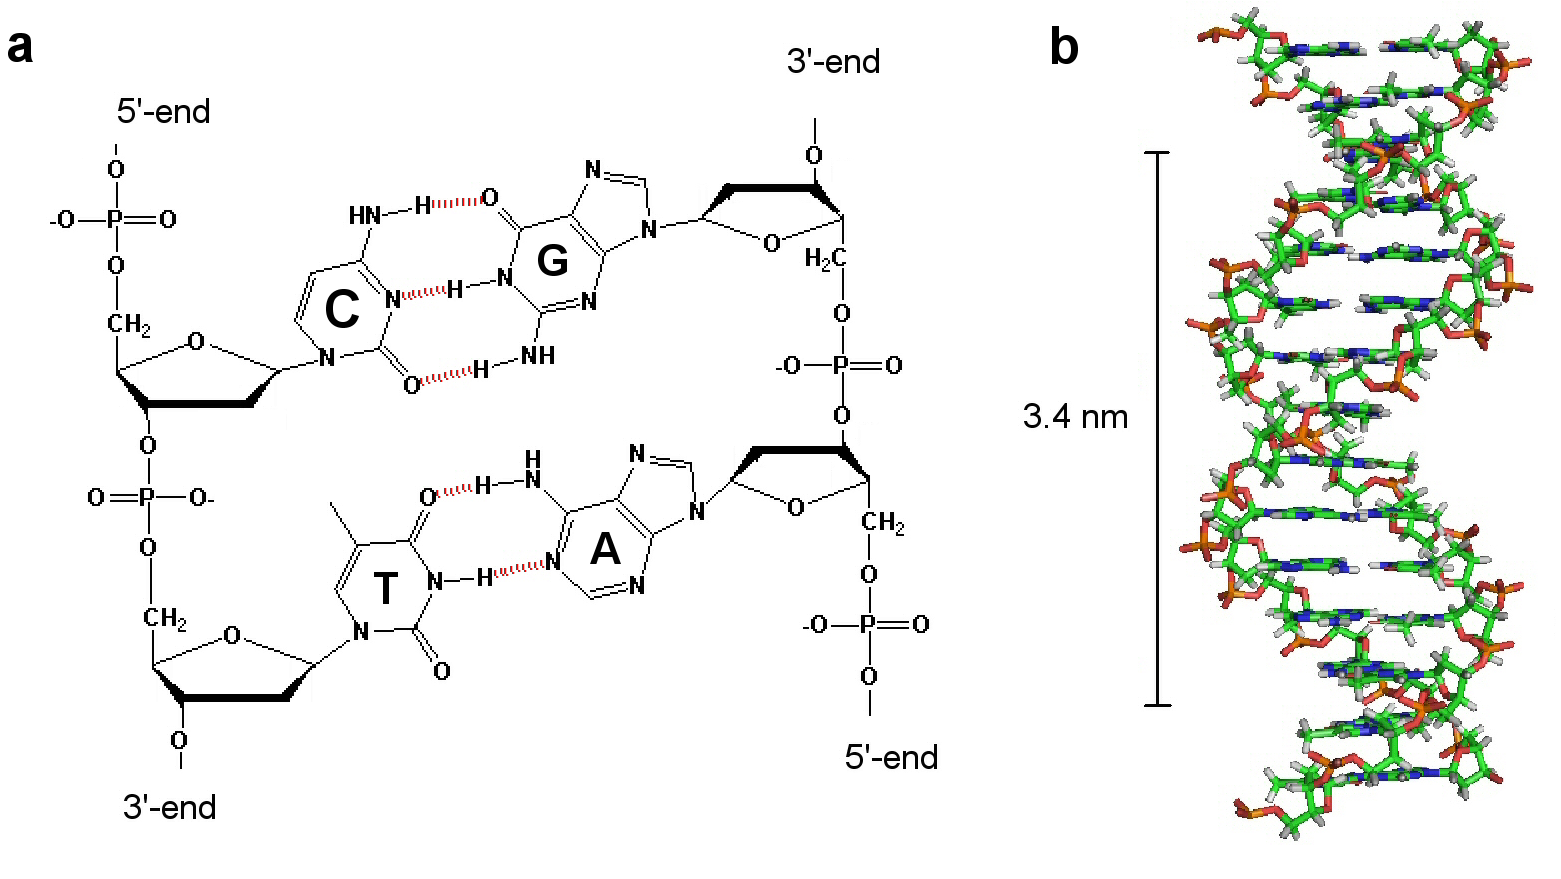
\includegraphics[width=0.88\textwidth]{adds//dna.png}
    \captionsetup{width=.95\textwidth}
    \caption{The DNA molecule. a) The chemical structure of DNA in which all four canonical nucleotides are shown in their base-pairing environment. b) The double-stranded B-DNA helix consisting of two antiparallel DNA strands hybridized as a result of Watson-Crick H-bonding between complementary bases in the two strands.}
    \label{Fig:chap_intro_dna}
\end{figure}

 The high specificity of Watson-Crick hydrogen bonding allows DNA molecules to be taken out of their biological context and exploited as building blocks in the construction of self-assembled nanoscale structures and functional devices (for recent reviews see e.g. \cite{Seeman2007,Seeman2010,Kuzuya2010,Nangreave2010,Torring2011,Shih2010,Aldaye2008}). The rigidity and chemical stability of the B-DNA helix makes this self-assembly approach highly attractive, in particular because it is relatively easy to design intermolecular nanostructures with predefined 2D- and 3D-shapes \cite{Tumpane2007,Rothemund2006,Simmel2008,Dietz2009,Douglas2009} and even a functionality such as mechanical movement \cite{Shin2004,Chen2004,Sherman2004,Li2002,Wickham2012,Wickham2011,Lund2010}, catalytic activity \cite{Baum2008,Chen2004a,Xiao2004} or drug transport\cite{Andersen2009,Douglas2012}.

\section{Fluorescence and Nucleic Acids}
 Over the years, fluorescence-based techniques have become invaluable tools in the molecular biosciences, and several new classes of fluorescent probes have recently been created to study biomolecules. The main advantage of fluorescence-based methods is that the natural nucleobases are virtually non-fluorescent \cite{Callis1983} enabling an outstanding signal-to-noise ratio when introducing fluorescence into DNA.

\subsection{Biocompatible Fluorescent Dyes}
 Fluorescent dyes may be introduced into DNA either non-covalently or covalently. Non-covalent DNA-binding dyes such as ethidium bromide bind to DNA by unspecific electrostatic interactions with the negatively charged backbone and/or by intercalation in between the hydrophobic bases.\cite{Ihmels2005,Armitage2005} In contrast, covalently attached fluorophores are usually tethered via a flexible linker to the DNA. This approach allows practically any fluorophore to be attached to the DNA at several different sites. The most popular probes are commercially available dyes such as the Cy-dyes and the Alexa-dyes which offer an unsurpassable overall brightness. These dyes are available in a variety spanning the entire visible spectrum.\cite{lifetechnologies} Alternative luminescent probes are e.g. lanthanides characterized by long excited state lifetimes\cite{Selvin2002} and inorganic semi-conductor quantum dots\cite{Giepmans2006,Medintz2005} characterized by their extremely high brightness.

 Using dyes attached externally to biomolecules has a number of disadvantages. Firstly, dyes often interact with their surrounding environment which may hamper the interpretation of experiments or change the fluorescence properties of the dye.\cite{Iqbal2008a,Neubauer2007,Norman2000,Sanborn2007,Sabanayagam2005a} Secondly, since external dyes reside on the outside of the biomolecular surface there is an inherent limitation in the kind of information obtainable from quantitative fluorescence experiments since the probes respond and report indirectly on the structure and dynamics of the biomolecule.

\subsection{Fluorescent Nucleobase Analogues}

 For studies involving nucleic acids, fluorescent nucleobase analogues constitute a different class of fluorophores that overcomes these problems (for reviews see \cite{Wilhelmsson2010,Sinkeldam2010,Rist2002,Hawkins2003,Okamoto2005,Wilson2006,Asseline2006,Loakes2007}). These probes can be inserted into DNA as a replacement for one of the natural bases mimicking the properties of the substituted base, in most cases without significantly affecting the DNA structure and function. In addition, when using nucleobase analogues the reporter can be positioned close to or even in the very site of interest when investigating DNA. Traditionally, the most utilized fluorescent nucleobase analogue has been 2-aminopurine (2-AP), an isomer of adenine capable of forming a base-pair with thymine and a less stable base-pair with cytosine.\cite{Freese1959} 2-AP is highly fluorescent in its free, monomeric form but is almost completely quenched in the base-stacking environment provided by dsDNA.\cite{Ward1969} This property has been exploited in probing the local structure and dynamics of DNA \cite{Guest1991,Xu1994,Millar1996} and in DNA-protein interactions that result in locally unwound strands \cite{Millar1996,Hochstrasser1994,Raney1994}. Other reported fluorescent base analogues include, but is not limited to, the pteridines\cite{Hawkins2001}, the expanded DNA bases\cite{Liu2004}, the wide DNA bases\cite{Lu2004}, the base-discriminating fluorescent base analogues\cite{Okamoto2003,Okamoto2003a,Okamoto2003b,Okamoto2005} and the emissive RNA alphabet by Tor and co-workers\cite{Shin2011}.

 The strict environment set by the DNA double helix in terms of H-bonding, base-stacking and steric hindrances, however, often affects the fluorescence properties of the fluorophore. As a result, fluorescent nucleobase analogues lag behind commercially available dye molecules in terms of overall brightness and spectral properties. Developing new fluorescent base analogues thus remains somewhat challenging. Common for all the fluorescent nucleobase analogues mentioned above are their sensitivity to the surrounding micro-environment, most often a significant quenching of fluorescence in dsDNA and a strong destabilizing effect of the DNA double helix. The highly relevant exception to these properties is the tricyclic cytosine (tC) family, 1,3-diaza-2-oxophenothiazine (tC), 1,3-diaza-2-oxophenoxazine (tC$^\mathrm{O}$) and 7-nitro-1,3- diaza-2-oxophenothiazine (tC$_\mathrm{nitro}$).\cite{Wilhelmsson2010,Wilhelmsson2001,Wilhelmsson2003,Sandin2005,Sandin2007,Sandin2008,Engman2004,Borjesson2009a,Preus2010} These base analogues are directly built upon the molecular framework of cytosine and extended by two extra rings (Figure \ref{Fig:chap_intro_tcprobes}). tC and tC$^\mathrm{O}$ both possess high fluorescence quantum yields ($\sim$0.2) and single-exponential lifetimes ($\sim$4-5 ns) in double-stranded DNA, relatively insensitive of neighbouring bases.\cite{Sandin2005,Sandin2008} In contrast, tC$_\mathrm{nitro}$ is virtually non-fluorescent at room-temperature but possess a red-shifted lowest energy absorption band compared to tC and tC$^\mathrm{O}$ which makes it perfectly suited as an energy transfer acceptor with tC or tC$^\mathrm{O}$ serving as the donor (Figure \ref{Fig:chap_intro_tcprobes}).\cite{Borjesson2009a,Preus2010} All of the tC probes adapt the position and orientation of the substituted cytosine base and stabilize the B-DNA double helix compared to regular cytosine.\cite{Engman2004,Sandin2008,Borjesson2009a}

 The tC family has a central role in this thesis. In Paper II and V they are subjected to a thorough photophysical characterization, while Paper III demonstrates their use in probing DNA structure and dynamics.

\begin{figure}
    \centering
        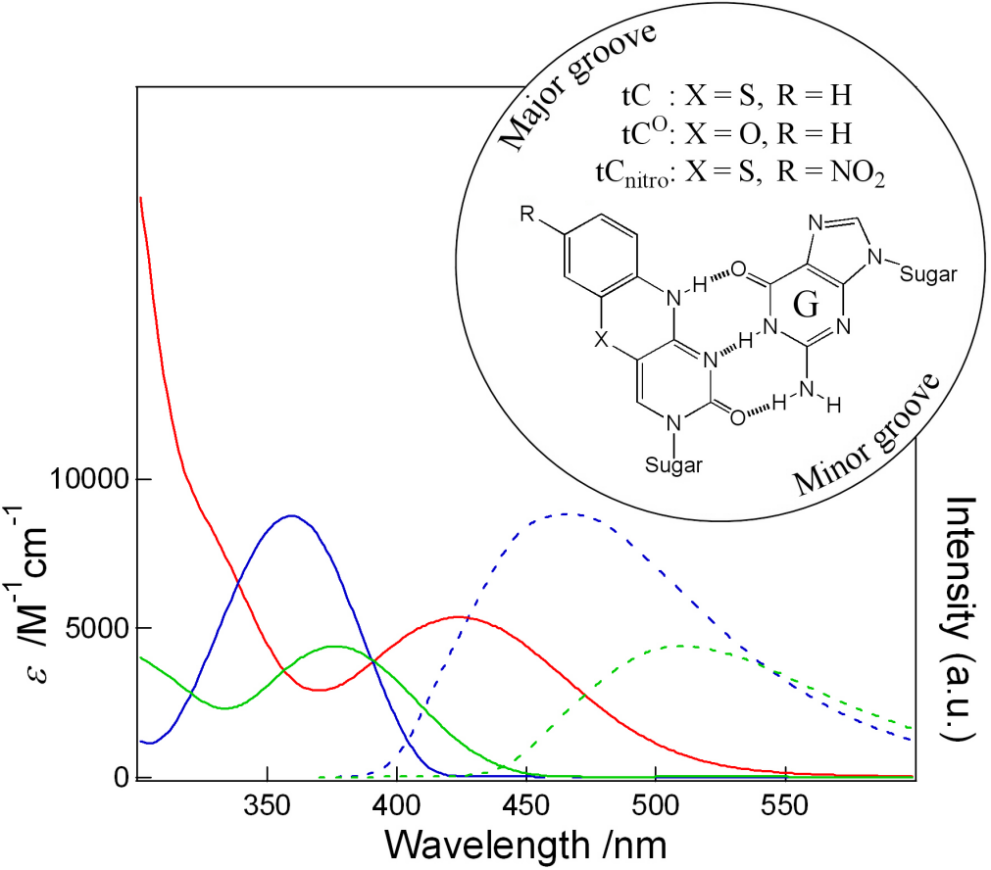
\includegraphics[width=0.65\textwidth]{adds//tcprobes.png}
    \captionsetup{width=.95\textwidth}
    \caption{UV-Vis absorption (full-drawn) and emission spectra (dashed) of the tricyclic cytosine analogues, tC (green), tC$^\mathrm{O}$ (blue) and tC$_\mathrm{nitro}$ (red). Insert: Chemical structures of the tC probes in the base-pairing environment with guanine.}
    \label{Fig:chap_intro_tcprobes}
\end{figure}

\subsection{FRET and Nucleic Acids}
 FRET is an energy transfer phenomenon that is widely used as a molecular ruler in the biosciences for probing nanoscale distances and molecular interactions (Figure \ref{Fig:chap_intro_fret}).\cite{Lak} The technique is usually performed by covalently labelling one or more biomolecules with two dyes: an energy donor and an acceptor. If the two probes are located within a distance related to the critical Förster distance of the pair (<10 nm) energy transfer can be induced between the two dyes which is observed as a decreased donor fluorescence yield, decreased donor excited state lifetime and, if the acceptor is emissive, an increased acceptor fluorescence yield. FRET may thus either serve as an "on/off" sensor of the relative location of the two dyes or as a quantitative ruler for determining the distance in between the FRET-pair. One of the aims of this thesis is to demonstrate that much more quantitative information, than a mere relative distance, can be gained from FRET experiments.

\begin{figure}
    \centering
        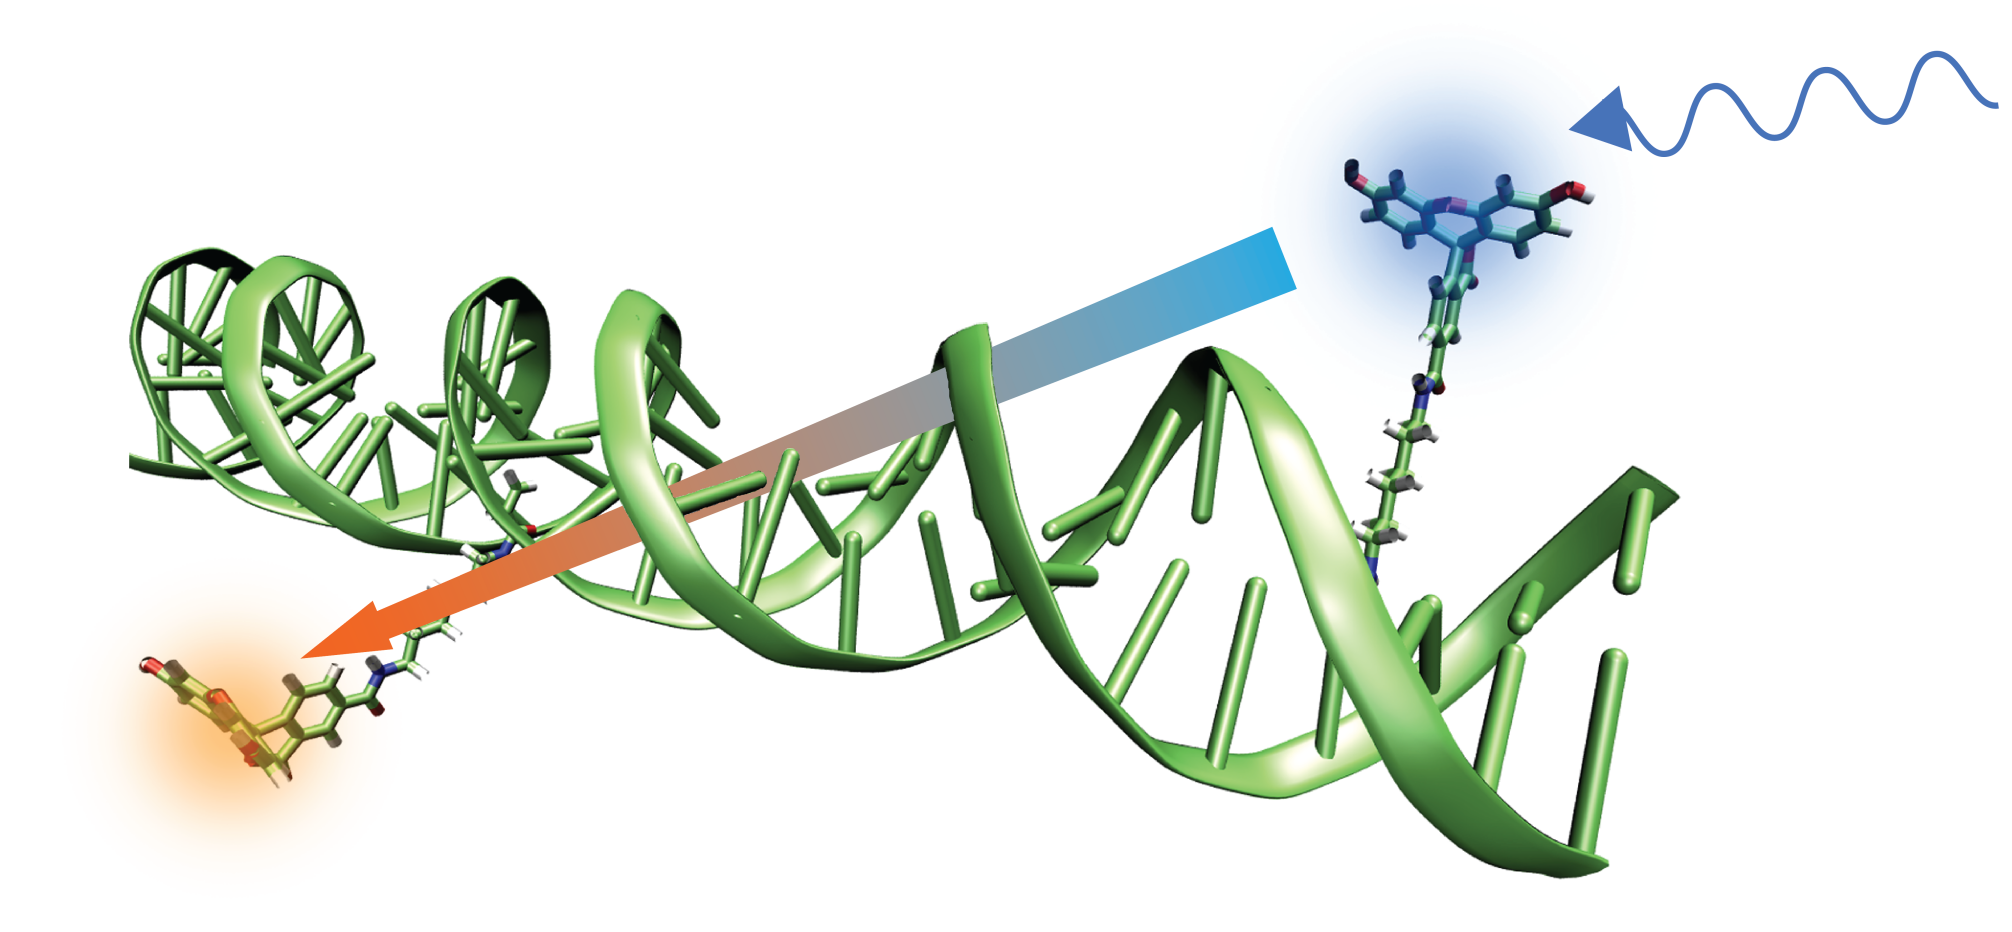
\includegraphics[width=0.8\textwidth]{adds//fret.png}
    \captionsetup{width=.95\textwidth}
    \caption{Illustration of FRET between two dyes tethered to DNA. After excitation of the donor this dye transfers its excitation energy to the acceptor located in close proximity. The FRET efficiency is highly distance dependent which makes the technique suited as a "molecular ruler" for probing nanoscale distances and molecular interactions.}
    \label{Fig:chap_intro_fret}
\end{figure}

\subsubsection{Historical View}
 FRET was first described by Förster in the 1940's as an interaction between two dipoles separated by a fixed distance, $r$, and oscillating in resonance.\cite{Foerster1948} By multiplying the probability that the two dipoles have the same resonance frequency with the rate of energy transfer when they do have the same resonance frequency, Förster derived the characteristic $r^{-6}$ dependency of the energy transfer rate constant (section \ref{sec:FRET}).\cite{Clegg1996} The FRET theory was continued to be discussed up to and during the 1970's\cite{Stryer1967,Dale1974,Dale1979}, however, it was not until late 1980's and early 1990's that FRET was exploited as a quantitative ruler to probe distances within nucleic acid structures.\cite{Murchie1989,Clegg1992b} In these studies, Lilley and co-workers determined the stereochemical arrangement of the four helices making up the Holliday junction, a four-stranded, four-way DNA junction which is an intermediate in genetic recombination. This late entrance of quantitative FRET in DNA was mainly due to difficulties in labeling nucleic acids site-specifically at that time. However, the DNA fluorescence toolbox has advanced greatly since then and custom dye-labelled oligonucleotides are now ordered and delivered on a day-to-day basis.\cite{lifetechnologies,GEHealthcare,GlenResearch,IDT,atdbio}

\subsubsection{FRET in Modern Applications}
 Today, FRET is used routinely as a technique to probe the structural states of nucleic acids. Particular advancement has occurred in recent years in the specific case where quantitative information about FRET-pair distances and nucleic acid three-dimensional structures is wanted from FRET experiments. The combination of multiple FRET-pair positions has provided quantitative insight into the three-dimensional structure of nucleic acids.\cite{Muschielok2008,Muschielok2011,Sabir2011,Sabir2012,Wozniak2008,Andrecka2008,Andrecka2009,Balci2011} Increasingly sophisticated techniques have been developed to model the uncertainty in the position and orientation of the dyes relative to the DNA.\cite{Muschielok2008,Sindbert2011,Rindermann2011} In addition to these improvements, the properties of many popular commercial FRET dyes attached to DNA are now known to some extent, such as the Cy-dyes\cite{Levitus2011,Norman2000,Sanborn2007,Iqbal2008a,Harvey2009,Harvey2009a}, FAM\cite{Noble2005,Unruh2005,Unruh2005a,Wang2004} and TAMRA\cite{Unruh2005,Unruh2005a,Wang2004,Vamosi1996,Stennett2012}. This knowledge is not only insightful but in fact vital in order to use FRET quantitatively on nucleic acid containing systems.

 An exciting development within FRET is the ability to monitor one molecule at a time, called single-molecule FRET (smFRET).\cite{Mollova2002,McKinney2004,Selvin2008,Roy2008,Joo2008} Single-molecule FRET techniques provide real-time insight into biomolecular structures and dynamics without hiding molecular heterogeneity behind an ensemble average. However, interpreting smFRET experiments into quantitative distances and dynamics is extremely difficult due to the low signal-to-noise ratio in such experiments, and methods are still being developed for analysing data from smFRET experiments quantitatively.\cite{Watkins2006,Gopich2005,Gopich2007,Gopich2009,Nir2006,Antonik2006,Kalinin2008,Kalinin2010} Multiparameter single-molecule fluorescence techniques, in which all possible ascertainable fluorescence parameters are monitored at the single-molecule level (intensity, anisotropy and lifetime), are extremely interesting in the context of quantitative smFRET.\cite{Sisamakis2010,Kuhnemuth2001,Kudryavtsev2012,Eggeling2006,Widengren2006,Laurence2005,Muller2005} Because all information required to interpret the measured signal into quantitative distances are acquired, such state-of-the art single-molecule techniques offer vast potential for providing detailed insight into the structure and dynamics of large biomolecules. Recently, single-molecule FRET has been used to probe the three-dimensional geometry of three-way DNA junctions\cite{Sabir2011,Sabir2012}, RNA polymerase II complexes\cite{Andrecka2008,Andrecka2009,Treutlein2012} and a helicase-DNA complex\cite{Balci2011} to name but a few.

 More references and information on recent advances within quantitative FRET is found in Paper I of this thesis.

 \paragraph{Base-base FRET.} In a previous study of ours (Appendix 1), a fluorescent nucleobase analogue FRET pair system was developed as an alternative to traditional, external FRET probes (Figure \ref{Fig:chap_intro_basefret}).\cite{Borjesson2009a} Since the base probes adapt the position and orientation of the canonical bases within double-stranded DNA this technique provides a number of advantages compared to traditional probes: First of all, the base probes can be positioned inside the very site of interest mimicking the behaviour of the substituted base and, thus, provides a means to probe the local base orientation and position at specific sites. Secondly, because both the orientation and position of the probes are highly constrained at the timescale of energy transfer this allows a higher degree of control of the orientation factor in the energy transfer process, and thus more detailed studies to be performed of three-dimensional nucleic acid structures without complications associated with linker flexibility.

 This latter point is demonstrated by the FRET efficiencies measured between the base analogue FRET-pairs positioned in B-DNA with distances varying from 2-13 base-pairs in between the FRET-pair (Figure \ref{Fig:chap_intro_basefretgraph}).\cite{Borjesson2009a} As the number of bases in between the pair increases both the distance as well as the relative orientation between the donor and acceptor gradually changes in a predictable manner. The result is a FRET curve decreasing with distance and, additionally, oscillating with a periodicity in phase with the helical periodicity of the B-DNA helix due to the change in orientation between the two transition dipole moments of the probes. The oscillation of the measured energy transfer efficiency in Figure \ref{Fig:chap_intro_basefretgraph} demonstrates the well-defined orientation of the base probes inside the DNA helix. The main disadvantage of base-base FRET is the complexity involved in the quantitative analysis of data from such experiments. A solution to this limitation is provided in this thesis.

\begin{figure}
    \centering
        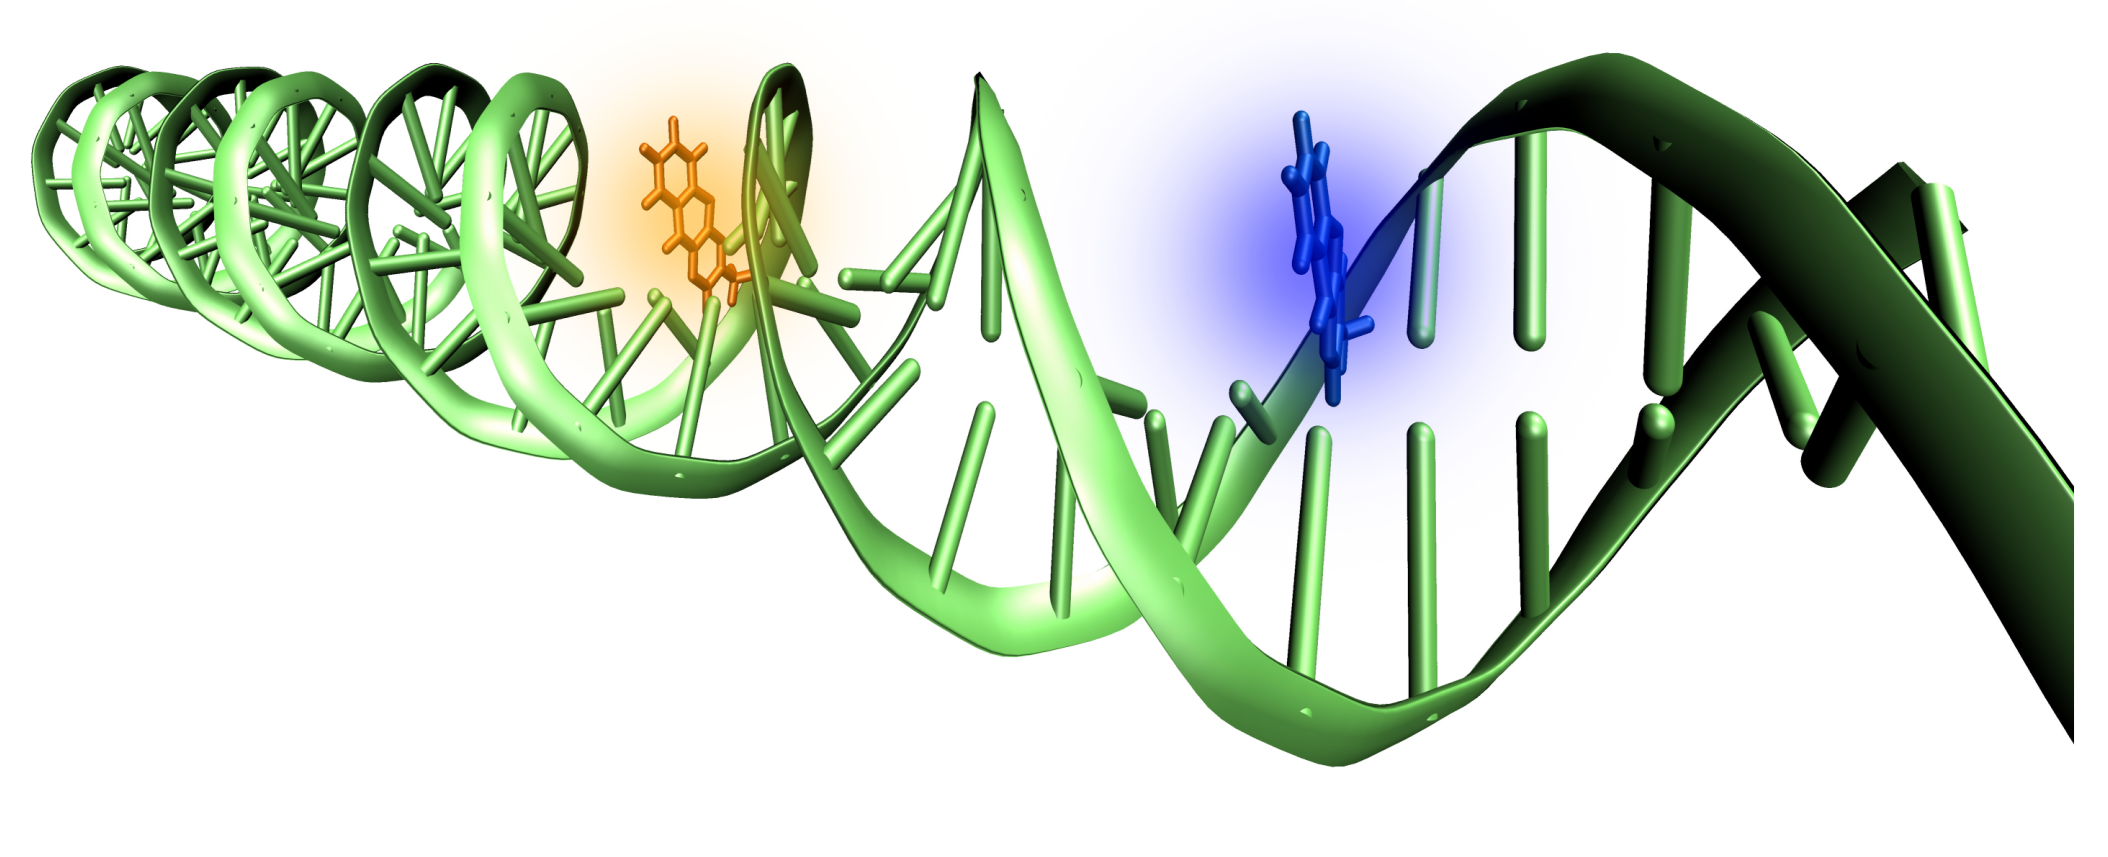
\includegraphics[width=0.7\textwidth]{adds//basefret.png}
    \captionsetup{width=.95\textwidth}
    \caption{Illustration of two base analogues positioned in B-DNA providing the foundation for base-base FRET.}
    \label{Fig:chap_intro_basefret}
\end{figure}
\begin{figure}
    \centering
        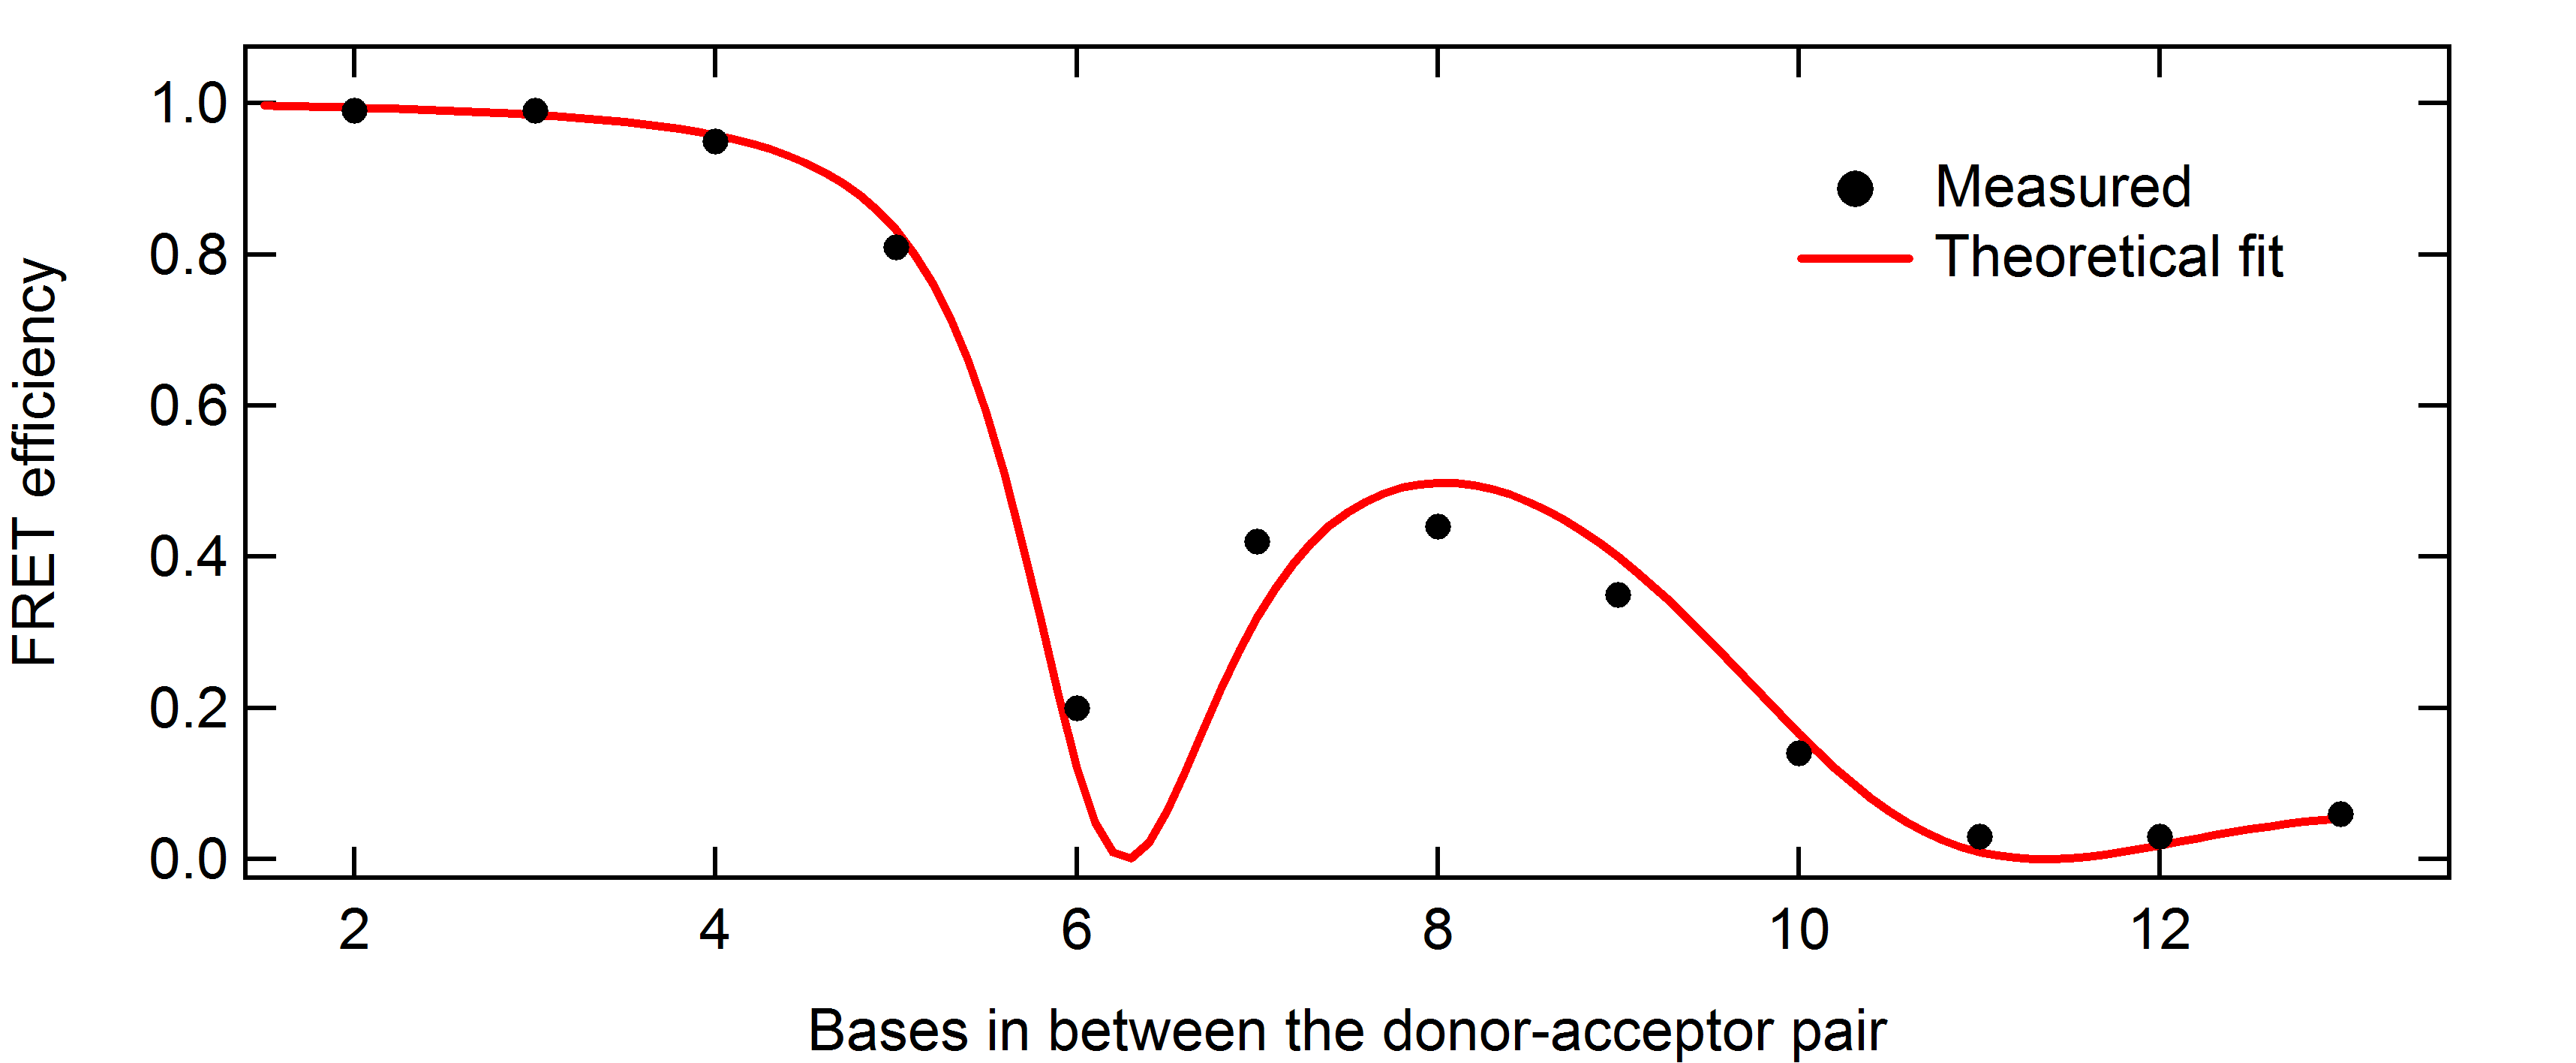
\includegraphics[width=0.7\textwidth]{adds//basefretgraph.png}
    \captionsetup{width=.95\textwidth}
    \caption{The FRET efficiencies measured between two base analogues positioned inside double-stranded B-DNA with varying inter-pair distance.\cite{Borjesson2009a} The red line is a theoretical fit based on the assumption of static transition dipoles positioned inside a perfect B-form helix with a twist of 36$^\circ$ and rise of 3.4 Å per dinucleotide step.}
    \label{Fig:chap_intro_basefretgraph}
\end{figure}

\subsubsection{Advantages and Drawbacks}
 Compared to higher resolution structural techniques like NMR spectroscopy\cite{Foster2007} and X-ray crystallography\cite{Holbrook2008}, FRET has the advantage of not being limited by the size of the system under investigation (unlike NMR), is solution-based (unlike crystallography) and, in addition, FRET is generally cheaper, faster, simpler and more sensitive. The drawbacks of FRET, however, are the dependency of the energy transfer on 1) probe orientation, which is very hard to control, and 2) the fluorescence quantum yield of the donor, which strongly depends on the interaction between the probe and its micro-environment and thus vary from sample to sample. While the second drawback can be accounted for using proper reference measurements (i.e. by using reference samples labelled with the donor only) the first drawback is more difficult to account for. Lower and upper boundaries of $\kappa^2$ can be estimated based on fluorescence anisotropy measurements\cite{Dale1974,Dale1979}, however, the exact $\kappa^2$-value or $\kappa^2$-distribution is practically impossible to obtain. This problem leads to an uncertainty in the distance deduced from FRET measurements.

 In this thesis, the novel FRET technique base-base FRET is developed and refined. It is demonstrated how the method facilitates an unprecedentedly high control of the position and orientation of the FRET probes and thus leads to more accurate and versatile quantitative FRET-based experiments.



\chapter{State--of--the--art}
\label{chap:art}
\textit{This chapter presents an overview to the state--of--the--art of \COPs{} and different approaches to tackle them. In Section~\ref{sec:combi} the definition of a \COP{} and its links with \CSPs{} (\csp) are introduced, where we concentrate the main efforts, and we give some examples. The basic techniques used to solve these problems are introduced: {\it \cp} (Section~\ref{sec:cp}) and {\it meta--heuristic methods} (Section~\ref{sec:meta}). We also present some advanced techniques like {\it hyper--heuristic methods} in Section~\ref{sec:hyper}, {\it hybridization} in Section~\ref{sec:hybrid}, {\it parallel computing} in Section~\ref{sec:parallel}, and {\it solvers cooperation} in Section~\ref{sec:cooperation}. Finally, before ending the chapter with a brief summary, we present {\it parameter setting techniques} in Section~\ref{sec:tunning}.}
\vfill
\minitoc
\newpage

%This chapter presents an overview to the state of the art of \COPs{} and different approaches to tackle them. In Section~\ref{sec:combi} the definition of a \CSP{} (\csp), emphasizing in the concept of \CSPs, where we concentrate our main efforts. Constraint propagation techniques are deterministic methods to attack these kind of problems (presented in Section~\ref{sec:progagation}), but in some cases they are incapable to solve them (they are mostly used to reduce the problem's search space or to prove it unsatisfiable). For that reason, the model presented in this thesis is based on \textit{meta-heuristic} methods (Section~\ref{sec:meta}). The \textit{Hybridization} approach combines different techniques in the same solution strategy, so the progresses in this field are exposed in Section~\ref{sec:hybrid}.

%The evolution of computer architecture is leading us toward massively multi-core computers for tomorrow, composed of thousands of computing units. A parallel model to solve \csps{} is the core of this work, and its advances, as well as those obtained in the field of \textit{cooperation between solvers}, are presented in Sections~\ref{sec:parallel} and \ref{sec:cooperation} respectively. Finally, this chapter presents in Section~\ref{sec:tunning} an overview of the progresses in the field of \textit{parameter settings}.  

\section{Combinatorial Optimization}\label{sec:combi}
Most of the \textit{Combinatorial Optimization} problems come from industrial and real world. We can find them in {\it Resource Allocations} \cite{Akplogan2011}, \textit{Task Scheduling} \cite{Sibbesen2008}, \textit{Master-keying} \cite{Espelage2000}, \textit{Traveling Salesman} and \textit{Knapsack} problems, among others, which are well-known examples of \cops{} \cite{Smith2005}. They are a particular case of \textit{optimization} problems, and their main goal is to find an optimum value (minimal or maximal, depending on the problem) for a discrete function $f$, called \textit{objective function}, involving a set variables $X = \left\{x_1, \dots, x_n\right\}$ defined over a set $D = \left\{D_1, \dots, D_n\right\}$ of discrete domains. These problems generally contain restrictions on the variables called \textit{constraints}, defining the set of forbidden combinations of values for variables in $X$, tacking into account the problem characteristics.

A \textit{configuration} $s\in D_1\times D_2\times\dots\times D_n$ is a combination of values for the variables in $X$. The fact of assigning values $v_i \in D_i$ to all variables in $x_i \in X$ is called \textit{evaluation}. When this evaluation is only performed to a given set of variables in $X$, we called it \textit{partial evaluation}. In combinatorial optimization, a \textit{feasible} configuration is a configuration fulfilling all constraints. Finally, a \textit{solution} $s^*$ to the problem is a configuration such that $f(s^*)$ is optimal.

In many practical cases, the main goal is not to find the optimal solution, but finding one feasible configuration. This is the case of \CSPs. Formally, the definition of a \csp{} is presented: 

\begin{definition}{\bf (Constraint Satisfaction Problem)}
\label{def:csp}
A \CSP{} (\csp, denoted by $\mathcal{P}$) is a triple $\langle X,D,C \rangle$, where:
\begin{itemize}
\item $X = \left\{x_1,\ldots,x_n\right\}$ is finite a set of variables,
\item $D = \left\{D_1,\ldots, D_n\right\}$ is the set of associated domains. Each domain $D_i$ specifies the set of possible values to the variable $x_i$. %is the set of associated domains to each variable in $X$,
\item $C = \left\{c_1,\ldots, c_m\right\}$ is a set of constraints. Each constraint is defined involving some variables from $X$, and specifies the possible combinations of values for these variables.
\end{itemize}
\end{definition}

In \csps, a solution is a configuration satisfying all constraints $c_i \in C$ (a feasible configuration). %We say that a configuration $s$ satisfies the constraint $c_i \in C$ if and only if $c_i$

\begin{definition}{\bf (Solution of a \csp)}
\label{solCSP}
Given a \csp{} $\mathcal{P}=\langle X,D,C \rangle$ and a configuration $s \in D_1\times D_2\times\dots\times D_n$ we say that it is a solution if and only if:	
\begin{equation*}
c_i\left(s\right)\text{ is true }\forall c_i \in C
\end{equation*}
\end{definition}

Let $Var(c_i)$ be the set of involved variables $\left\{x_1, \dots, x_p\right\}$ in the constraint $c_i$, with $p\leq n$. Then, $c_i\left(s\right)$ denotes the evaluation using the values from the configuration $s$ to the variables $Var(c_i)$. The set of all solutions of $\mathcal{P}$ is denoted by $\mathnormal{Sol}(\mathcal{P})$.

A \csp{} can be considered as a special case of \cops, where the objective function is to reduce to the minimum the number of violated constraints in the model. A solution is then obtained when the number of violated constraints reach the value zero. 

\etal{Galinier} present in \cite{Galinier04} a general approach for solving \csps{}. In this work, authors present the concept of {\it penalty functions} that we pick up in order to write a \csp{} as an \textit{Unrestricted Optimization Problem} (UOP). This formulation was useful in this thesis for modeling the tackled benchmarks. In this formulation, the objective function of this new problem must be such that its set of optimal solutions is equal to the solution set of the original (associated) \csp.

\begin{definition}{\bf (Local penalty function)}
\label{def:local_cost}
Let a {\bf \csp} $\mathcal{P}\langle X,D,C \rangle$ and a configuration $s$ be. We define the operator {\bf local penalty function} as follow: 
\begin{equation*}
\begin{array}{l}
	\omega_i:D\left(X\right)\times 2^{D\left(X\right)}\rightarrow\mathbb{R}^+\text{ where: }\\
	\omega_i\left(s,c_i\right)=\left\{
	\begin{array}{lll}
	0 & \text{ if } & c_i(s)\text{ is true }\\
	k \in \mathbb{R}^+ \setminus {0} & \text{ otherwise } &
	\end{array}
	\right.
\end{array}
\end{equation*}
where $D\left(X\right) = D_1\times D_2 \times\dots\times D_n$
\end{definition}

This penalty function defines the cost of a configuration with respect to a given constraint, so if $\omega_i\left(s,c_i\right)=k$ we say that the configuration $s$ has a local cost $k$ with respect to the constraint $c_i$. In consequence, we define the \textit{global penalty function}, to define the cost of a configuration with respect to all constraint on a \csp:

\begin{definition}{\bf (Global penalty function)}
\label{def:global_cost}
Let a {\bf \csp} $\mathcal{P}\langle X,D,C \rangle$ and a configuration $s$. We define the operator {\bf global penalty function} as follows: 
\begin{equation*}
\begin{array}{l}
\Omega:D\left(X\right)\times 2^{D\left(X\right)}\rightarrow\mathbb{R}^+ \text{ where: }\\
\Omega\left(s,C\right)=\displaystyle\sum_{i=1}^{m}{\omega_i\left(s,c_i\right)}
\end{array}
\end{equation*}
\end{definition}

This global penalty function defines the cost of a configuration with respect to a given set of constraints, so if $\Omega\left(s,C\right)=k$ we say that the configuration $s$ has a cost $k$ with respect to $C$. We can now formulate a \CSP{} as an {\it unrestricted optimization problem}:

\begin{definition}{\bf (CSP's Associated Unrestricted Optimization Problem)}
\label{def:ass_CSP}
Given a {\bf \csp} $\mathcal{P}\langle X,D,C \rangle$ we define its associated Unrestricted Optimization Problem $\mathcal{P}_{opt}\langle X,D,C,f \rangle$ as follows: 
\begin{equation*}
\begin{array}{l}
\displaystyle\min_{X} f\left(X,C\right)\\
\text{Where:  } f\left(X,C\right) \equiv \Omega\left(X,C\right) \text{ is the objective function to be minimized over the variable } X
\end{array}
\end{equation*}
\end{definition}

It is important to note that a given $s$ is optimum if and only if $f\left(s,C\right) = 0$, which means that $s$ satisfies all the constrains in the original \csp{} $\mathcal{P}$. This work focuses in solving the \CSP{} using this formulation.

%An \textit{Optimization Problem} consists in finding the best solution among all possible ones, subject or not, to a set of constraints, depending on whether it is a restricted or an unrestricted problem. The suitable values for the involved variables belong to a set called {\it domain}. When this domain contains only discrete values, we are facing a \COP, and its goal is to find the best possible solution satisfying a global criterion, named {\it objective function}. {\it Resource Allocations} \cite{Akplogan2011}, \textit{Task Scheduling} \cite{Sibbesen2008}, \textit{Master-keying} \cite{Espelage2000}, \textit{Traveling Salesman}, \textit{Knapsack Problem}, among others, are well-known examples of \cops{} \cite{Smith2005}.

\section{Constraint programming}\label{sec:cp}
\csps{} find a lot of "real-world" applications in the industry. In practice, these problems are tackled through different techniques. One of the most popular is \textit{constraint programming}, a combination of three main ingredients: \begin{inparaenum}[i)] \item a declarative model of the problem, \item constraint reasoning techniques like \textit{filtering} and \textit{propagation}, and \item search techniques. \end{inparaenum} This field is a famous research topic developed by the field of artificial intelligence in the middle of the 70's, and a programming paradigm since the end of the 80's.

Modeling a constrained problem, to be solved using \cp{} techniques, means properly choosing variables and their domains, and a right and efficient representation of the constraints set, aiming to declare as explicitly as possible, the solutions space. On the right election of the problem's model depends not only finding the solution, but also doing it in a fast and efficient way.

For modeling \csps{}, two tools can be highlighted. {\sc MiniZinc} is a simple but expressive constraint programming modeling language which is suitable for modeling problems for a range of solvers. It is the most used language for codding \csps{} \cite{Nethercote}. {\sc XCSP} is a readable, concise and structured XML-like language for coding \csps. This format allows to represent constraints defined either extensionally or intensionally. %Is not more used than {\sc MiniZinc} but although 
It was mainly used as the standard in the {\it International Constraint Solver Competition} (ended in 2009), and the {\it ICSC} dataset is for sure the biggest dataset of \csps{} instances existing today. \new{{\sc XCSP3}\footnote{XCSP3 website: \href{www.xcsp.org}{www.xcsp.org}} is the last upgrade of this format and it is available on Internet. Compact and easy to parse, {\sc XCSP3} is able to capture the structure of the problem models, and identifying syntactic and semantic groups of constraints. It introduces a number of features that make it able to enclose practically all constraints that can be found in major constraint solvers \cite{Boussemart2016}}. 

Constraint reasoning techniques are filtering algorithms applied for each constraint to prune provably infeasible values from the domain of the involved variables. This process is called \textit{constraint propagation}, and they are methods used to modify a \CSP{} in order to reduce its variables domains, and turning the problem into one that is equivalent, but \new{with a smaller search space, hence} usually easier to solve \cite{ChristianBessiere2006}. The main goal is to choose one (or some) constraint(s) to enforce certain consistency levels in the constraints. Achieving global consistency is desirable, because only using brute force algorithms one can reach a solution, but this is computationally very costly and intractable. %extremely hard to obtain. 
For that reason, some other consistency levels, easier to achieve, have been defined, like for example, \textit{arc consistency} and \textit{bound consistency}, which means trying to find values in the variables domain which make constraint unsatisfiable, in order to remove them from the domain. The applied procedure to reduce the variable domains is called \textit{reduction function}, and it is applied until a new, "smaller" and easier to solve problem is obtained, and it can not be further reduced: a \textit{fixed point}. Local consistency restrictions on the filtering algorithms are necessary to ensure not loosing solution during the propagation process.

%Before presenting these two consistency levels mentioned before, is imperative to define some notations. 
We said that a variable $x \in c$, if it is involved into the constraint $c$. Let the set $Var(c) = \{x_1\dots x_k\}$ the set of variables  involved into a constraint $c$ be, denoted by $Var(c)$. Then, a constraint $c$ is called \textit{arc consistent} if for all $x_i \in Var(c)$ with $1\leq i\leq k$, and for all $v_j \in D_j$ with $1\leq j\leq \left\|D_j\right\|$:
\[
\exists (v_1, \dots, v_{i-1}, v_{i+1},\dots, v_k) \in D_1\times\dots\times D_{i-1}\times D_{i+1}\times\dots\times D_k
\]
such that $c(v_1, \dots, v_k)$ is fulfilled. In other words, $c$ is arc consistent if for each value of each variable, there exist values for the other variables fulfilling $c$. In that case, we said that each value in the domain of $x_i$ has a \textit{support} in the domain of the other variables.

We denote by $Bnd(D_i) = \left\{\min(D_i), \max(D_i)\right\}$ the bounds of the domain $D_i$. Then, a constraint is \textit{bound consistent} if for all $x_i \in Var(c)$ with $1\leq i\leq k$, and for all $v_j \in Bnd(D_j)$ with $1\leq j\leq 2$:
\[
\exists (v_1, \dots, v_{i-1}, v_{i+1},\dots, v_k) \in Bnd\left(D_1\right)\times\dots\times Bnd\left(D_{i-1}\right)\times Bnd\left(D_{i+1}\right)\times\dots\times Bnd\left(D_k\right)
\]
such that $c(v_1, \dots, v_k)$ is fulfilled. It means that each bound (min/max) in the domain of $x_i$ has a support in the bounds (min/max) of the other variables. As we can notice that arc consistency is a stronger property, but heavier to enforce.

Apt and Monfroy have proposed in \cite{Apt} and \cite{Monfroy}, respectively, a formalization of constraint propagation through \textit{chaotic iterations}, which is a technique that comes from numerical analysis to compute limits of iterations of finite sets of functions, and adapted for computer science needs for naturally explain constraint propagation \cite{Chazan1969, Cousot1977}. Another approach is presented by Monfroy in \cite{Monfroy2000}, a coordination-based chaotic iteration algorithm for constraint propagation, which is a scalable, flexible and generic framework for constraint propagation using coordination languages, not requiring special modeling of \csps. Zoeteweij provides an implementation of this algorithm in {\sc DICE} (Distributed Constraint Environment) \cite{Zoeteweij2003} using the {\sc Manifold} coordination language. Coordination services implement existing protocols for constraint propagation, termination detection and splitting of \csps. {\sc DICE} combines these protocols with support for parallel search and the grouping of closely related components into cooperating solvers.

Another implementation of constraint propagation is proposed by \etal{Granvilliers} in \cite{Granvilliers2001}, using composition of reductions. It is a general algorithmic approach to tackle strategies that can be dynamically tuned with respect to the current state of constraint propagation, using composition operators. A composition operator models a sub--sequence of an iteration, in which the ordering of application of reduction functions is described by means of combinators for sequential, parallel or fixed--point computation, integrating smoothly the strategies to the model. This general framework provides a good level of abstraction for designing an object-oriented architecture of constraint propagation. Composition can be handled by the {\it Composite Design Pattern} \cite{DP_Composite}, supporting inheritance between elementary and compound reduction functions. The propagation mechanism uses the {\it Observer (Listener) Design Pattern} \cite{DP_Observer}, that makes the connection between domain modifications and re--invocation of reduction functions (event-based relations between objects); and the generic algorithm has been implemented using the {\it Strategy Design Pattern} \cite{DP_Strategy}, that allows to parametrize parts of algorithms.

A propagation engine prototype with a \textit{Domain Specific Language} (DSL) was implemented by \etal{Prud'homme} in \cite{Prudhomme2013}. It is a solver--independent language able to configure constraint propagations at the modeling stage. The main contributions are a DSL to ease configure constraint propagation engines, and the exploitation of the basic properties of DSL in order to ensure both completeness and correctness of the produced propagation engine. %, like:	
%\begin{inparaenum}[i)]%\begin{itemize}
%	\item {\it Solver independent description}: The DSL does not rely on specific solver requirements (but assuming that solvers provide full access to variable and propagator properties), 
%	\item {\it Expressivity}: The DSL covers commonly used data structures and characteristics, 
%	\item {\it Extensibility}: New attributes can be introduced to make group definition more concise. New collections and iterators can provide new propagation schemes, 
%	\item {\it Unique propagation}: The top-bottom left-right evaluation of the DSL ensures that each arc is only represented once in the propagation engine.
%\end{inparaenum}%\end{itemize}
Some characteristics are required to fully benefit from the DSL. Due to their positive impact on efficiency, modern constraint solvers already implement these techniques:
\begin{inparaenum}[i)] %\begin{itemize}
	\item Propagators are discriminated thanks to their priority (deciding which propagator to run next): lighter propagators (in the complexity sense) are executed before heavier ones.
	\item A controller propagator is attached to each group of propagators.
	\item Open access to variable and propagator properties: for instance, variable cardinality, propagator arity or propagator priority.
\end{inparaenum}%\end{itemize}
To be more flexible and more accurate, they assume that all arcs from the current \textit{CSP}, are explicitly accessible. This is achieved by explicitly representing all of them and associating them with {\it watched literals} \cite{Gent2006} (controlling the behavior of variable--value pairs to trigger propagation) or {\it advisors} \cite{Lagerkvist2007} (a method for supporting incremental propagation in propagator--centered setting). %{\it Advisors} in \cite{Lagerkvist2007} are used to modify propagator state and to decide whether a propagator must be propagated or "scheduled". 

Most of the times, we can not solve \csps{} only applying constraint propagation techniques. It is necessary to combine them with search algorithms. The complete search process consists in testing all possible configurations in an ordered way. Each time a partial evaluation is executed (evaluating just a set of variables), new constraints are posted, meaning that the propagation process can be relaunched. The simplest approach is using a backtracking search. It can be seen as performing a depth--first traversal of a search tree. This search tree is generated as the search progresses and represents alternative choices that may have to be examined in order to find a solution. Constraints are used to check whether a node may possibly lead to a solution of the \csp{} and to prune subtrees containing no solutions. A node in the search
tree is a \textit{dead-end} if it does not lead to a solution. Differences between searches lies in the selection criteria of the order of variables to be evaluated, and the order of the values to be assigned to variables. A \textit{static} search strategy is based on selecting the variable with me minimum index, to be evaluated first with the minimum value of its domain. Using this search, the \textit{tree structure} of the search space does not change, but is good for testing propagators. A \textit{dynamic} search strategy is based on selecting the variable with me minimum domain element, to be evaluated first with the minimum value of its domain. In this search strategy, propagators affect the variable selection order. A classical search strategy is based on selecting the variable with me minimum domain size, to be evaluated first with any values of its domain. Based on the \textit{first fail} principle which tells "\textit{Focus first on the variable that is more likely to cause a fail}",  this strategy works pretty well in many cases because by branching early on variables with a few value, the search tree becomes smaller.

In the field of \cp{} we can find a lot of solvers, able to solve constrained problems using these techniques. As examples, we can cite {\sc Cplex}\footnote{CPLEX Optimizer, available at: \href{http://www.ilog.com/products/cplex/}{http://www.ilog.com/products/cplex/}}, \textit{OR-tools}\footnote{Google Optimization Tools, available at: \href{https://developers.google.com/optimization/}{https://developers.google.com/optimization/}}, {\sc Gecode} and \choco. {\sc Cplex} is an analytical decision support toolkit for rapid development and deployment of optimization models using mathematical and constraint programming, to solve very large, real-world optimization problems. {\sc Gecode} is an efficient open source environment for developing constraint-based system and applications, that provides a modular and extensible constraint solver \cite{Gecode}, written in C++ (winner of all gold medals in the \textit{MiniZinc Challenge} from 2008 to 2012). During the formation phase of this PhD, we had the opportunity to perform some pedagogical experiments using two other important and recognized solvers: \textit{OR-tools} and \choco. The \textit{OR-tools} is an open source, portable and documented software suite for combinatorial optimization. It contains an efficient  constraint programming solver, used internally at Google, where speed and memory consumption are critical.

\choco{} is a free and open-source tool written in java, to describe hard combinatorial problems in the form of \csps{} and solving them using \CP{} techniques. Mainly developed by people at \'Ecole des Mines de Nantes (France), is a solver with a nice history, wining some awards, including seven medals in four entries in the \textit{MiniZinc Challenge}. This solver uses multi-thread approach for the resolution, and provides a problem modeler able to manipulate a wide variety of variable types. This problem modeler accepts over 70 constraints, including all classical arithmetical constraints, the possibility of using boolean operations between constraints, table constraints, i.e. defining the sets of tuples that verify the intended relation for a set of variables and a large set of useful classical global constraints including the \textit{alldifferent} constraint, the global \textit{cardinality} constraint, the \textit{cumulative} constraint, among others. \choco{} also contains a {\sc MiniZinc} and \textit{XCSP} instance parser. 
\choco{} can either deal with satisfaction or optimization problems. The search can be parameterized using a set of predefined variable and value selection heuristics, and also the variable and/or value selectors can be parametrized \cite{Jussien2008, Prudhomme2016}.

Although \cp{} techniques have shown very good results solving constrained problems, the search space in practical instances becomes intractable for them. For that reason, these constrained problems are mostly tackled by {\it meta-heuristic methods} or hybrid approaches. %, like \textit{Monte Carlo Tree Search} methods, which combine precision (tree search) with randomness (meta-heuristic) showing good results in artificial intelligence for games \cite{Chaslot2008, Browne2012}.

\section{Meta-heuristic methods}\label{sec:meta}
{\it Meta-heuristic} methods are algorithms generally applied to solve problems deprived of satisfactory problem-specific algorithms to solve them. They are general purpose techniques widely used to solve complex optimization problems in industry and services, in areas ranging from finance to production management and engineering, with relatively few modifications: \begin{inparaenum}[i)] \item they are nature-inspired (based on some principles from physics or biology), \item they involve random variables as an stochastic component, therefore approximate and usually non-deterministic, \item and they have several parameters that need to be fitted \cite{Dreo2006}.\end{inparaenum} 

A meta-heuristic method is formally defined as an iterative process which guides a subordinate heuristic by combining different concepts for \textit{exploration} (also called \textit{diversification}) i.e. guiding the search process through a much larger portion of the search space; and \textit{exploitation} (also called \textit{intensification}) i.e. guiding the search process into a limited, but promising, region of the search space \cite{Osman1996}.

In contrast with tree-search based methods, which are subject to combinatorial explosion (required time to find solutions of NP-hard problems increases exponentially with respect to the problem size), they do dot perform an ordered and complete search. For that reason they are not able to provide a proof that the optimal solution will be found in a finite (although often prohibitively large) amount of time. Meta-heuristics are therefore developed specifically to find an "\textit{acceptably good}" solution "\textit{acceptably}" fast. In the case of \csps, finding a feasible solution is enough, for that reason, these methods have been proven to be effective solving these kind of problems.

Sometimes meta-heuristics use domain-specific knowledge in the form of heuristics controlled by an upper level strategy. Nowadays more advanced meta-heuristics use search experience to guide the search \cite{Blum2003}.

Meta-heuristics are divided into two groups: % \cite{Boussaid2013}: 
\begin{enumerate}%\begin{inparaenum}[i)]
    \item {\it Single Solution Based:} more exploitation oriented, intensifying the search in some specific areas. This work focuses its attention on this first group.
    \item {\it Population Based:} more exploration oriented, identifying areas of the search space where there are (or where there could be) the best solutions. % \cite{Maturana2012, Reeves2010, Dorigo2010}.
\end{enumerate} %\end{inparaenum}

\subsection{Single Solution Based Meta-heuristic}

% you will focus on the first group => this is your thesis topic
Methods of the first group are also called {\it trajectory methods}. They usually start from a candidate configuration $s$ (usually random) inside the search space, and then iteratively make local moves consisting of applying some local modifications to $s$ to create a set of configuration called \textit{neighborhood} $\mathcal{V}\left(s\right)$, and selecting a new configuration $s'\in \mathcal{V}\left(s\right)$, following some criteria, to be the new candidate solution for the next iteration. This process is repeated until a solution for the problem is found. These methods can be seen as an extension of \textit{local search methods} \cite{Boussaid2013}. Local search methods are the most widely used approaches to solve \COPs{} because they often produces high--quality solutions in reasonable time \cite{Voss2012}.
 
{\it Simulated Annealing} (SA) \cite{Nikolaev2010} is one of the first algorithms with an explicit strategy to escape from local minima. It is a method inspired by the annealing technique used by metallurgists to obtain a "well ordered" solid state of minimal energy. Its main feature is to allow moves resulting in solutions of worse quality than the current solution under certain probability, in order to scape from local minima, which is decreased during the search process \cite{Blum2003}. As an example of an implementation of this algorithm obtaining good results, it can be cited a work presented by \etal{Anagnostopoulos} in \cite{Anagnostopoulos2006} which is an adaptation of a SA algorithm (TTSA) for the Traveling Tournament Problem (TPP) that explores both feasible and infeasible schedules that includes advanced techniques such as strategic oscillation to balance the time spent in the feasible and infeasible regions by varying the penalty for violations; and reheats (increasing the temperature again) to balance the exploration of the feasible and infeasible regions and to escape local minima.

{\it Tabu Search} (TS) \cite{Gendreau2010}, is a very classic meta-heuristic for \COPs. It explicitly maintains a history of the search, as a short term memory keeping track of the most recently visited solutions, to scape from local minima, to avoid cycles, and to deeply explore the search space. A TS meta-heuristic guides the search on the approach presented in \cite{IvanDotu2007} by Iván Dotú and Pascal Van Hentenryck to solve instances of the \textit{Social Golfers} problem, showing that local search is a very effective way to solve this problem. The used approach does not take symmetries into account, leading to an algorithm which is significant simpler than constraint programming solutions. 

{\it Guided Local Search} (GLS) \cite{Christos2010} consists of dynamically changing the objective function to change the search landscape, helping the search escape from local minima. The set of solutions and the neighborhood are fixed, while the objective function is dynamically changed with the aim of making the current local optimum less attractive \cite{Blum2003}. \etal{Mills} propose in \cite{Mills2000} an implementation of a GLS, which is used to solve the satisfiability (SAT) problem, a special case of a \csp{} where variables take booleans values and constraints are disjunctions of literals (i.e. variables or theirs negations).

The \textit{Variable Neighborhood Search} (VNS) is another meta-heuristic that systematically changes the neighborhood size during the search process. This neighborhood can be arbitrarily chosen, but often a sequence $\left|\mathcal{N}_1\right|<\left|\mathcal{N}_2\right|< \dots<\left|\mathcal{N}_{k_{max}}\right|$ of neighborhoods with increasing cardinality is defined. The choice of neighborhoods of increasing cardinality yields a progressive diversification of the search \cite{PierreNenad,Blum2003}. \etal{Bouhmala} introduce in \cite{Bouhmala2015} a \textit{generalized Variable Neighborhood Search} for \COPs, where the order in which the neighborhood structures are selected during the search process offers a more effective mechanism for diversification and intensification. %and in \cite{Burke2010} is presented a model combining integer programming and VNS for \textit{Constrained Nurse Rostering} problems.

{\it Greedy Randomized Adaptive Search Procedures} (GRASP) is an iterative randomized sampling technique in which each iteration provides a solution to the target problem at hand through two phases (constructive and search). The first one constructs an initial solution via an adaptive randomized greedy function. This function construct a solution performing partial evaluations using values of a restricted candidate list (RCL) formed by the best values, incorporating to the current partial solution values resulting in the smallest incremental costs (the greedy aspect of the algorithm). The value to be incorporated into the partial solution is randomly selected from those in the RCL (the random aspect of the algorithm). Then the candidate list is updated and the incremental costs are reevaluated (the adaptive aspect of the algorithm). The second phase applies a local search procedure to the constructed solution in to find an improvement \cite{Feo95}. GRASP does not make any smart use of the history of the search process. It only stores the problem instance and the best found solution. That is why GRASP is often outperformed by other meta-heuristics \cite{Blum2003}. However, \etal{Resende} introduce in \cite{Resende2009} some extensions like alternative solution construction mechanisms and techniques to speed up the search are presented.

Many other implementations of local search algorithms have been presented with good results. {\it Adaptive Search} is an algorithm based local search method, taking advantage of the structure of the problem in terms of constraints and variables. It uses also the concept of \textit{penalty function}, based on this information, seeking to reduce the \textit{error} (a projected cost of a variable, as a measure of how responsible is the variable in the cost of a configuration) on the worse variable so far. It computes the penalty function of each constraint, then combines for each variable the \textit{errors} of all constraints in which it appears. This allows to choose the variable with the maximal \textit{error} will be chosen as a "culprit" and thus its value will be modified for the next iteration with the best value, that is, the value for which the total error in the next configuration is minimal \cite{Diaz, Codognet2001, Caniou14}. In \cite{Munera2015} \etal{Munera} based their solution method in Adaptive Search to solve the \textit{Stable Marriage with Incomplete List and Ties} problem \cite{Iwama1999}, a natural variant of the \textit{Stable Marriage Problem} \cite{Gale1962}, using a cooperative parallel approach. Michel and Van Hentenryck propose in \cite{Michel2002} a constraint-based, object-oriented architecture to significantly reduce the development time of local search algorithms. This architecture consists of two main components: a declarative component which models the application in terms of constraints and functions, and a search component which specifies the meta-heuristic, illustrated using {\sc Comet}, an optimization platform that provides a Java-like programming language to work with constraint and objective functions \cite{Comet, Michel2005}, supporting the local search architecture. It also provides abstraction features to make a clean separation between the model an the search (promoting the reusing of the later) and novel control structures to implement nondeterminism.

\subsection{Population Based Meta-heuristic}

In the second group of meta-heuristic algorithms we can find methods based on population sets. These methods do not work with a single configuration, but with a set of configurations named {\it population}. They were not part of the main investigation of this thesis, so we will not get into details, but we think it is fair to mention some of the most important methods.

The most popular algorithms in this group are population-based methods. They are related to \begin{inparaenum}[i)] \item \textit{Evolutionary Computation} (EC), inspired by the "Darwin's principle", where only the best adapted individuals will survive, where a population of individuals is modified through recombination and mutation operators, and \item \textit{Swarm Intelligence} (SI), where the idea is to produce computational intelligence by exploiting behaviors of social interaction~\cite{Boussaid2013}.\end{inparaenum} 

Algorithms based on evolutionary computation have a general structure. Every iteration of the algorithm corresponds to a \textit{generation}, where a population of candidate solutions (called individuals) to a given problem, is capable of reproducing and is subject to genetic variations and environmental pressure that causes natural selection. New solutions are created by applying recombination, by combining two or more selected individuals (parents) to produce one or more new individuals (the offspring). Mutation can be applied allowing the appearance of new traits in the offspring to promote diversity. The fitness (how good the solutions are) of the resulting solutions is evaluated and a suitable selection strategy is then applied to determine which solutions will be maintained into the next generation. As a termination condition, a predefined number of generations (or function evaluations) of simulated evolutionary process is usually used. The evolutionary algorithm's operators are another branch of study, because they have to be selected properly according to the specific problem, because they play an important roll in the algorithm behavior \cite{Maturana2012}.

Probably the most popular evolutionary algorithms are {\it Genetic Algorithms} (GA) \cite{Reeves2010}, where operators are based on the simulation of the genetic variation  process to achieve individuals (solutions in this case) more adapted. GAs are usually differently implemented according to the problem: representation of solution (chromosomes), selection strategy, type of crossover (the recombination operator) and mutation operators, etc. The most common representation of the chromosomes is a fixed-length binary string, because simple bit manipulation operations allow the easy implementation of crossover and mutation operations.

Swarm intelligence (SI) based methods are inspired by the collective behavior in society of groups different form of live. SI systems are typically made up of a population of simple element, capable of performing certain operations, interacting locally with one another and with their environment. These elements have very limited individual capability, but in cooperation with others, they can perform many complex tasks necessary for their survival. Ant colony optimization, Particle Swarm Optimization and Bee Colony Optimization are examples to this approach.

{\it Ant Colony optimization} algorithms are inspired by the behavior of real ants. Ants searching for food, initially explore the area surrounding the nest by performing a randomized walk. Along the path between food source and nest, ants deposit a pheromone trail on the ground in order to mark some promising path that should guide other ants to the food source. After some time, the shortest path between the nest and the food source has a higher concentration of pheromone, so it attracts more ants \cite{Dorigo2010}.

\textit{Particle Swarm optimization} uses the metaphor of the flocking behavior of birds to solve optimization problems. Each element of the swarm is a candidate solution to the problem, stochastically generated in the search space, and they are connected to some others elements called \textit{neighbors}. It is represented by a velocity, a location in the search space and has a memory which helps it to remember its previous best position. This values describe the \textit{influence} of each element over its neighbors \cite{Poli2007}.

\textit{Bee Colony optimization} consists of three groups of bees: employed bees, onlookers and scout bees. A food source is a possible solution to the problem. Employed bees are currently exploiting a food source. They exploit the food source, carry the information about food source back to the hive and share it with onlooker bees. Onlookers bees wait in the hive for the information to be shared with the employed bees to update their knowledge about discovered food sources. Scouts bees are always searching for new food sources near the hive. Employed bees share information about the nectar amount of a food source by dancing in the designated dance area inside the hive. This information represents the quality of the solution. The nature of dance is proportional to the nectar content of food source. Onlooker bees watch the dance and choose a food source according to the probability proportional to the quality of that food source. In that sense, good food sources attract more onlooker bees. Whenever a food source is fully exploited, all employed bees associated with it abandon the food source, and become scouts \cite{Gao2012}.

\section{Hyper-heuristic Methods}\label{sec:hyper}
\textit{Hyper-heuristics} are automated methodologies for selecting or generating meta-heuristics algorithms to solve hard computational problems \cite{Chakhlevitch2008}. This can be achieved with a learning mechanism that evaluates the quality of the algorithm solutions, in order to become general enough to solve new instances of a given problem. \textit{Hyper-heuristics} are related with the \textit{Algorithm Selection Problem}, so they establish a close relationship between a problem instance, the algorithm to solve it and its performance \cite{Ryser-welch}. Hyper-heuristic frameworks are also known as \textit{Algorithm-Portfolio}--based frameworks. Their goal is predicting the running time of algorithms using statistical regression. Then the fastest predicted algorithm is used to solved the problem until a suitable solution is found or a time-out is reached \cite{Leyton-Brown2003}.

This approach have been followed for solving constrained problems. {\sc Hyperion}$^2$ \cite{Brownlee2014} is a Java framework for meta-- and hyper-- heuristics which allows the analysis of the trace taken by an algorithm and its constituent components through the search space. It promotes interoperability via component interfaces, allowing rapid prototyping of meta- and hyper-heuristics, with the potential of using the same source code in either case. It also provides generic templates for a variety of local search and evolutionary computation algorithms, making easier the construction of novel meta- and hyper-heuristics by hybridization (via interface interoperability) or extension (subtype polymorphism). {\sc Hyperion}$^2$ is faithful to "{\it only pay for what you use}", a design philosophy that attempts to ensure that generality doesn't necessarily imply inefficiency. \textit{hMod} is inspired by the previous frameworks, but using a new object-oriented architecture. It encodes the core of the hyper-heuristic in several modules, referred as algorithm containers. \textit{hMod} directs the programmer to define the heuristic using two separate XML files; one for the heuristic selection process and the other one for the acceptance criteria \cite{Urra2013}.

\textit{Evolving evolutionary algorithms} are specialized hyper-heuristic method which attempt to readjust an evolutionary algorithm to the problem needs. An evolutionary algorithm (EA) discover the rules and knowledge to find the best algorithm to solve a problem. In \cite{Diosan2009} \etal{Dio\c{s}an} use linear genetic programming and multi-expression genetic programming to optimize the EA solving unimodal mathematical functions and another EA to adjust the sequence of genetic and reproductive operators. A solution consists of a new evolutionary algorithm capable of outperforming genetic algorithms when solving a specific class of unimodal test functions. An different but interesting point of view is presented in \cite{Samulowitz2013}, where \etal{Samulowitz} present \textit{Snappy}, a \textit{Simple Neighborhood-based Algorithm Portfolio} written in \textit{Python}. It is a very resent framework that aims to provide a tool able to improve its own performances through on-line learning. Instead of using the traditional off-line training step, a neighborhood search predicts the performance of the algorithms. It incorporates available knowledge coming from portfolio's runs, by considering the following ways incrementally: \begin{inparaenum}[1-] \item Every time a test instance is considered, it is added to the current set of training instances. \item After selecting an algorithm for a given test instance, the actual runtime information for the selected algorithm on this instance is added to the data set. It means that the difference between neighborhoods of different algorithms represent how often algorithms will be selected. \end{inparaenum} Other interesting idea is proposed by \etal{Swan} in {\sc Templar}, a framework to generate algorithms changing predefined components using hyper-heuristics methods \cite{Swan2015}.

\section{Hybridization}\label{sec:hybrid}
The \textit{Hybridization} approach is the one who combine different approaches into the same solution strategy, and recently, it leads to very good results in the constraint satisfaction field. For example, constraint propagation may find a solution to a problem, but they can fail even if the problem is satisfiable, because of its local nature. At each step, the value of a small number of variables are changed, with the overall aim of increasing the number of constraints satisfied by this assignment, and applying other techniques to avoid local solutions, for example adding a stochastic component to choose variables to affect. Integrations of global search (complete search) with local search have been developed, leading to hybrid algorithms. 


An interesting hybridization point of view, is the integration of operations research into constraint programming. \etal{Fontaine} use in \cite{Fontaine2014} a generalization of the optimization paradigm \textit{Lagrangian relaxation}, to relax the hard constraints into the objective function, and applying them into constraint-programming and local search models. It combine the concepts of constraint violation (typically used in constraint programming and local search) and constraint satisfiability (typically used in mathematical programming). Hooker J.N. presents in \cite{Hooker2006} a detailed description of how operation research models like mixed integer linear programming (MILP) models (which can themselves be relaxed), Lagrangian relaxations, and dynamic programming models can be applied to constraint programming. 

Hooker J.N. presents in \cite{Hooker2012} some ideas to illustrate the common structure present in exact and heuristic methods, to encourage the exchange of algorithmic techniques between them. The goal of this approach is to design solution methods ables to smoothly transform its strategy from exhaustive to non-exhaustive search as the problem becomes more complex.

In \cite{El-Ghazali2013} a taxonomy of hybrid optimization algorithms is presented in an attempt to provide a mechanism to allow qualitative comparison of hybrid optimization algorithms, combining meta-heuristics with other optimization algorithms from mathematical programming, machine learning and constraint programming.

Monfroy et al. present in \cite{Monfroya,Monfroyb} a general hybridization framework, proposed to combine complete constraints resolution techniques with meta-heuristic optimization methods in order to reduce the problem through domain reduction functions, ensuring not loosing solutions. Other interesting ideas are {\sc Templar}, a framework to generate algorithms changing predefined components using hyper-heuristics methods \cite{Swan2015}; and {\it ParadisEO}, a framework to design parallel and distributed hybrid meta-heuristics showing very good results \cite{Cahon2004}, including a broad range of reusable features to easily design evolutionary algorithms and local search methods.

Another technique has been developed, the called {\it autonomous search}, based on the supervised or controlled learning. This systems improve their functioning while they solve problems, either  modifying their internal components to take advantage of the opportunities in the search space, or to adequately chose the solver to use ({\it portfolio point of view}) \cite{WhatIsAuto}.

In \cite{Amadini2014} is proposed another portfolio-based technique, \textit{time splitting}, to solve optimization problems. Given a problem \textit{P} and a schedule $Sch = \left[(\Sigma_1, t_1),\dots,(\Sigma_n, t_n)\right]$ of \textit{n} solvers, the corresponding time-split solver is defined as a particular solver such that:  
\begin{enumerate}[label=\alph*)]
\item runs $\Sigma_1$ on \textit{P} for a period of time $t_1$, 
\item then, for $i = 1,\dots, n-1$, runs $\Sigma_{i+1}$ on \textit{P} for a period of time $t_{i+1}$ exploiting or not the best solution found by the previous solver $\Sigma_i$ $t_i$ units of time.
\end{enumerate}

% COMENTAR 
%Nowadays there exists some tools to face this kind of problems. We can cite {\sc Choco}, an open source java constraint programming library \cite{Jussien2008}; ; ; {\sc Adaptive Search}, a constraint-based local search methods \cite{Diaz}; among others.

% Citas estas cosas en la parte donde propongo mi modelado :D

%COMENTAR   
%There exist also tools for modeling \textit{CSP} problems. Some of them intent to be a standards in terms of problem modeling.  Codding the problems using one of these tools (or both), it gives us the advantage of solving them using many solvers that support those languages. Furthermore, developing our own solver, it is also interesting to use them because we can test and compare our results using a wide range of available problems. 

In \cite{Amadini} is proposed a tool (\texttt{xcsp2mzn}) for converting problem instances from the format  \cite{Committee} to {\sc MiniZinc} that is a simple but expressive constraint programming modeling language which is suitable for modeling problems for a range of solvers. It is the most used language for codding \csps{} \cite{Nethercote}. The second contribution of this work is the development of \texttt{mzn2feat} a tool to extract static and dynamic features from the {\sc MiniZinc} representation, with the help of the {\sc Gecode} interpreter, and allows a better and more accurate selection of the solvers to be used according to the instances to solve. Some results are showed proposing that the performances that can be obtained using these features are competitive with state of the art on \csp{} portfolio techniques. 

%\nocite{Choco, Comet, CometPascal, Gecode, XCSP, Features, Minizinc, X10}

\section{Parallel computing}\label{sec:parallel}
Despite advances previously presented, hard instances of many problems are still complicated to solve through these techniques. Thanks to \textit{parallel computing}, we have been capable of going one step further in solving \csps. Parallel computing is a way to solve problems using several computation resources at the same time. It is a powerful alternative to solve problems which would require too much time by using sequential algorithms \cite{Grama2003}. %That is why this field is in constant development and it is the topic where we put most of our effort. 

Since the late 2000's all processors in modern machines are multi-core. Massively parallel architectures, previously expensive and so far reserved for super--computers, become now a trend available to a broad public through hardware like the Xeon Phi or GPU cards. The power delivered by massively parallel architectures allow us to treat faster constrained problems \cite{Borkar2007}. However this architectural evolution is a non-sense if algorithms do not evolve at the same time: the development and the implementation of algorithms should take this into account and tackling problems with very different methods, changing the sequential reasoning of researchers in Computer Science \cite{Hill2008, Sanders2014}. 

In the literature on parallel constraint solving \cite{Gent}, two main limiting factors on performance are addressed: \begin{inparaenum}[1-] \item inter-process communication overheads (explained in details in Section~\ref{sec:cooperation}), and \item the \textit{Amdahl}'s law. \end{inparaenum} The Amdahl's law of parallel computing states that the \textit{speed-up} of a parallel algorithm is limited by the fraction of the program that must be executed sequentially. It means that adding more processors may not make the program run faster. It assumes that some percentage of the program or code cannot be parallelized ($T_{sequential}$), and states that the ratio called speed-up of $T_{sequential}$ over $1 - T_{Sequential} = T_{parallel}$ is bounded by $1\setminus T_{sequential}$ when the number of processors $P \rightarrow \infty$:

\begin{equation}\label{amdahl}
Speed-Up = \frac{T_{sequential}}{T_{parallel}} \leq \frac{1}{T_{sequential}}
\end{equation}

%\item parallelizing the search process,  
%\item parallel and distributed arc-consistency, 
%\item multi-agent and cooperative search and
%\item combined parallel search and parallel consistency.

Another issue, usually underestimated, is the codification. Writing efficient code for parallel machines is less trivial, as it usually deals with low-level APIs such as OpenMP and message-passing interfaces (MPI), among others. However, years of experience have shown that using those frameworks is difficult and error-prone. Usually many undesired behaviors (like deadlocks) make parallel software development very slow compared to sequential approaches. In that sense, Falcou proposes in \cite{Falcou2009} a programming model: \textit{parallel algorithmic skeletons} (along with a C++ implementation called {\sc Quaff}) to make parallel application development easier. This model is a high-order pattern to hide all low-level, architecture or framework dependent code from the user, and provides a decent level of organization. {\sc Quaff} is a skeleton-based parallel programming library, which has demonstrated its efficiency and expressiveness solving some application from computer vision. It relies on C++ template meta-programming to reduce the overhead traditionally associated with object-oriented implementations of such libraries allowing some code generation at compilation time. \etal{Cahon} also propose {\it ParadisEO}, a framework to design parallel and distributed hybrid meta-heuristics showing very good results, including a broad range of reusable features to easily design evolutionary algorithms and local search methods \cite{Cahon2004}.

%The contribution in terms of hardware has been crucial, achieving powerful technologies to perform large--scale calculations. 

The development of techniques and algorithms to solve problems in parallel focuses principally on three fundamental aspects: 
\begin{enumerate}%\begin{inparaenum}[i)]
    \item {\it Problem subdivision},
    \item {\it Search parallelization} and %{\it Scalability} and
    \item {\it Inter-process communication}.
\end{enumerate}%\end{inparaenum}
They all pursue the same objective: achieving good levels of \textit{scalability}. Scalability is the ability of a system to handle the increasing growth of workload. 
%A system which has improved over time its performance after adding work resources, and it is capable of doing it proportionally is called {\it scalable}. 
%The increase has not been only in terms of calculus resources, but also in the amount of sub-problems coming from the sub-division of the original problem. The more we can divide a problem into smaller sub-problems, the faster we can solve it \cite{Hill}. 
\textit{Adaptive Search} is a good example of local search method that can scale up to a larger number of cores, e.g., a few hundreds or even thousands of cores \cite{Diaz}. For this algorithm, an implementation of a cooperative multi-walks strategy has been published by \etal{Munera} in \cite{Munera}. In this framework processes are grouped in teams to achieve search intensification, which cooperate with others teams through a head node (process) to achieve search diversification. Using an adaptation of this method, authors propose a parallel solution strategy able to solve hard instances of \textit{Stable Marriage with Incomplete List and Ties Problem} quickly. This technique has been combined in \cite{Munera2016} with an \textit{Extremal Optimization} procedure: a nature-inspired general-purpose meta-heuristic \cite{Boettcher2000}.
	
The issue of subdividing a given problem in some smaller sub-problems is sometimes not easy to address. Even when we can do it, the time needed by each process to solve its own part of the problem is rarely balanced. For that reason it is imperative to apply some complementary techniques to tackle this problem, taking into account that sometimes, the more a problem can be sub-divided, the more balanced will be the execution times of the process \cite{Hill}.%\cite{Rezgui2013, Hill}. 
In \cite{Arbab2000} Arbab and Monfroy propose a mechanism to create sub-\csps{} (whose union contains all the solutions of the original \csp) by splitting the domain of the variables. The coordination is achieved though communication between processes. The contribution of this work is explained in details in Section~\ref{sec:cooperation}. 

In \cite{Yasuhara2015} \etal{Yasuhara} propose a new search method called \textit{Multi-Objective Embarrassingly Parallel Search} (MO--EPS) to solve multi-objective optimization problems, based on: 
\begin{inparaenum}[i)]
	\item Embarrassingly Parallel Search (EPS), where the initial problem is split into a number of independent sub-problems, by partitioning the domain of decision variables \cite{Regin2014}; and %\cite{Rezgui2013, Regin2014}; and
	\item Multi-Objective optimization adding cuts (MO--AC), an algorithm that transforms the multi-objective optimization problem into a feasibility one, searches a feasible solution and then the search is continued adding constraints to the problem until either the problem becomes infeasible or the search space gets entirely explored \cite{Kotecha2010}.
\end{inparaenum}
Multi-objective optimization problems involve more than one objective function to be optimized simultaneously. Usually these problems do not have an unique optimal solution because there exist a trade-off between one objective function and the others. For that reason, in a multi-objective optimization problem, the concept of \textit{pareto optimal} points is used. A pareto optimal point is a solution that improving one or some objective function values, implies the deterioration of at least one of the other objective function. %A collection of pareto optimal points defines a pareto front.

Related to parallelizing the search process, we can find two main approaches. First, the {\it single walk} approach, in which all the processes try to follow the same path towards the solution, solving their corresponding part of the problem, with or without cooperation (communication). The other is known as {\it multi walk}, consisting of the execution of various independent processes to find the solution. Each process applies its own strategies (portfolio approach) or simply explores different places inside the search space. Although this approach may seem too trivial and not so smart, it is fair to say that it is in fashion due to the good obtained results using it \cite{Diaz}.

\etal{Kishimoto} present in \cite{Kishimoto2013} a comparison between \textit{Transposition-table Driven Scheduling} (TDS) and a parallel implementation of a best-first search strategy (Hash Distributed A$^*$), that uses the standard approach of \textit{work stealing} for partitioning the search space. This technique is based on maintaining a local work queue, (provided by a root process through hash-based distribution that assign an unique processor to each work) accessible to other process that "steal" work from it if they become unoccupied. Authors use MPI, the paradigm of \textit{Message Passing Interface} that allows parallelization, not only in distributed memory based architectures, but also in shared memory based architectures and mixed environments (clusters of multi-core machines) \cite{Grama2003a}. The same approach is used by Jinnai and Fukunaga in \cite{Jinnai} to evaluate \textit{Zobrist Hashing}, an efficient hash function designed for table games like Chess and Go, to mitigate communication overheads.

In \cite{Arbelaez2012} \etal{Arbelaez} present a study of the impact of space-partitioning techniques on the performance of parallel local search algorithms to tackle the \textit{K-Medoids} clustering problem. Using a parallel local search method, this work aims to improve the scalability of the sequential algorithm, which is measured in terms of the quality of the solution within a given timeout. Two main techniques are presented for domain partitioning: first, {\it space-filling curves}, used to reduce any N-dimensional representation into a one-dimension space (this technique is also widely used in the nearest-neighbor-finding problem \cite{Chen2005}); and second, {\it k-Means} algorithm, one of the most popular clustering algorithms \cite{Berkhin2002}.

An interesting work is presented by \etal{Truchet} in \cite{Truchet02}, which is an estimation of the speed-up (a performance prediction of a parallel algorithm) through statistical analysis of its sequential algorithm is presented. Using this approach it is possible to have a rough idea of the resources needed to solve a given problem in parallel. In this work, authors study the parallel performances of \textit{Las Vegas} algorithms \cite{Babai1979} (randomized algorithms whose runtime might vary from one execution to another, even with the same input) under independent multi-walk scheme, and predict the performances of the parallel execution from the runtime distribution of their sequential runs. These predictions are compared to actual speed--ups obtained for a parallel implementation of the same algorithm and show that the prediction can be quite accurate.

The other important aspect in parallel computing is the inter-process communication, also called \textit{solver cooperation} and it is treated in the next section.

%A lot of studies have been published around this topic. A parallel solver for numerical \csps{} is presented in \cite{Ishii2014} showing good results scaling on a number of cores.
%We can find in \cite{Diaz2012} a survey of the different parallel programming models and available tools, emphasizing on their suitability for high-performance computing.

%Some other efforts have been allocated in the exploitation of the power of calculus provided by the massively parallel architecture of the Graphic Processing Unit (GPU). In \cite{Arbelaez} are presented  implementations of efficient (and very fast) constraint-based local search solvers using GPU.
%\nocite{GPU}

\section{Solvers cooperation}\label{sec:cooperation}
The interaction between solvers exchanging information is called {\it solver cooperation}. %and it is very popular in this field due to their good results. 
Its main goal is to improve some kind of limitations or inefficiency imposed by the use of unique solver. In practice, each solver runs in a computation unit, i.e. thread or processor. The cooperation is performed through inter--process communication, by using different methods: \textit{signals}, asynchronous notifications between processes in order to notify an event occurrence; \textit{semaphore}, an abstract data type for controlling access, by multiple processes, to a common resource; \textit{shared memory}, a memory simultaneously accessible by multiple processes; \textit{message passing}, allowing multiple programs to communicate using messages; among others.

Many times a close collaboration between process is required, in order to achieve the solution. But the first inconvenient is the slowness of the communication process. Some works have achieved to identify what information is viable to share. One example is the work presented by \etal{Hamadi} in \cite{Hamadi2012}, where an idea to include low-level reasoning components in the SAT problems resolution is proposed, dynamically adjusting the size of shared clauses to reduce the possible blow up in communication. This approach allows to perform the clause-sharing, controlling the exchange between any pair of processes.

This is a very changeling field, that is way we can find a lot of interesting ideas in the literature to improve parallel solutions through solver cooperation techniques. 

\etal{Kishimoto} present in \cite{Kishimoto2009} a parallelization of an algorithm A$^*$ (Hash Distributed A$^*$) for \textit{optimal sequential planning} \cite{Schmegner2004}, exploiting distributed memory computers clusters, to extract significant speed--ups from the hardware. In classical planning solving, both the memory and the CPU requirements are main causes of performance bottlenecks, so parallel algorithms have the potential to provide required resources to solve changeling instances. 

In \cite{Pajot2003} Pajot and Monfroy present a paradigm that enables the user to properly separate strategies combining solver applications, from the way the search space is explored in solver cooperations. The cooperation must be supervised by the user, through {\it cooperation strategy language}, which defines the solver interactions during the search process.

{\sc Meta--S} is an implementation of a theoretical framework proposed in \cite{Frank2003} by \etal{Franc}, which allows to tackle constrained problems, through the cooperation of arbitrary domain--specific constraint solvers. Through its modular structure and its extensible strategy specification language, it also serves as a test--bed for generic and (meta--)~solving strategies, which are problem--specific and employed to minimize the incurred cooperation overhead. Treating the employed solvers as black boxes, the meta--solver takes constraints from a global pool and propagates them to the individual solvers, which are in return requested to provide newly gained information (i.e., constraints) back to the meta--solver, through variable projections. The major advantage of this approach lies in the ability to integrate arbitrary, new or pre--existing constraint solvers, to form a system that is capable of solving complex mixed--domain constraint problems, at the price of increased cooperation overhead. This overhead can however be reduced through more intelligent and/or problem--specific cooperative solving strategies. 

%In \cite{Frank2003} have been presented an implementation of the meta-solver framework which coordinates the cooperative work of arbitrary pluggable constraint solvers. This approach intents to integrate arbitrary, new or pre--existing constraint solvers, to form a system capable of solving complex mixed--domain constraint problems. The existing increased cooperation overhead is reduced through problem-specific cooperative solving strategies.

%{\sc Hyperion} \cite{Brownlee2014} is an already mentioned framework for meta-- and hyper--heuristics built with the principle of interoperability, generality by providing generic templates for a variety of local search and evolutionary computation algorithms; and efficiency, allowing rapid prototyping with the possibility of reusing source code.

Arbab and Monfroy propose in \cite{Arbab2000} a technique to guide the search by splitting the domain of variables. A \textit{master} process builds the network of variables and domain reduction functions, and sends this information to the \textit{worker} processes. Workers concentrate their efforts on only one sub-\csp{} and the master collects solutions. The main advantage is that by changing only the search agent, different kinds of search can be performed. The coordination process is managing using the {\sc Manifold} coordination language \cite{Arbab1995}.

A component-based constraint solver in parallel is proposed in \cite{Zoeteweij} by Zoeteweij and Arbab. In this work, a parallel solver coordinates autonomous instances of a sequential constraint solver, which is used as a software component. The component solvers achieve load balancing of tree search through a time-out mechanism. It is implemented a specific mode of solver cooperation that aims at reducing the turn-around time of constraint solving through parallelization of tree search. The main idea is trying to solve a \csp{} before a time-out. If it cannot find a solution, the algorithm defines a set of disjoint sub-problems to be distributed among a set of solvers running in parallel. The goal of the time-out mechanism is to provide an implicit load balancing: when a solver is idle, and there are no subproblems available, another solver produces new sub-problems when its time-out elapses.

%{\sc Manifold} is a strongly-typed, block-structured, event-driven language for managing events, dynamically changing interconnections among sets of independent, concurrent and cooperative processes. A {\sc Manifold} application consists of a number of processes running on a heterogeneous network. Processes in the same application may be written in different programming languages. {\sc Manifold} has been successfully used in a broad range of applications \cite{Arbab1995}.

\etal{Munera} present in \cite{Munera} a new paradigm that includes cooperation between processes, in order to improve the independent multi-walk approach. In that case, cooperative search methods add a communication mechanism to the independent walk strategy, to share or exchange information between solver instances during the search process. This proposed framework is oriented towards distributed architectures based on clusters of nodes, with the notion of {\it teams} running on nodes and controlling several search engines ({\it explorers}) running on cores. All teams are distributed and thus have limited inter--node communication. This tool provides diversification through communication between teams, extending the search to different regions of the search space. Intensification is ensured through communication between explorers, and it is achieved swarming to the most promising neighborhood found by explorers. %This framework is oriented towards distributed architectures based on clusters of nodes, where teams are mapped to nodes and explorers run on cores. 
This framework was developed using the {\it X10 programming language}, which is a novel language for parallel processing developed by IBM Research, giving more flexibility than traditional approaches, e.g. MPI communication package.

A similar approach is presented by \etal{Guo} in \cite{Guo2010}, exploring principles of diversification and intensification in portfolio--based parallel SAT solving. To study their trade--off, they define two roles for the computational units. Some of them classified as {\it masters} perform an original search strategy, ensuring diversification. The remaining units, classified as {\it slaves} are there to intensify their master's strategy. 
%There are some important questions to be answered:
%\begin{inparaenum}[i)]
%	\item what information should be given to a slave in order to intensify a given search effort?, 
%	\item how often, a subordinated unit has to receive such information? and 
%	\item the question of finding the number of subordinated units and their connections with the search efforts? 
%\end{inparaenum}
Results lead to an original intensification strategy which outperforms the best parallel SAT solver {\it ManySAT}, and solves some open SAT instances.

\etal{Hamadi} propose in \cite{Hamadi2011} the first {\it Deterministic Parallel DPLL} (a complete, backtracking-based search algorithm for deciding the satisfiability of propositional logic formulas in conjunctive normal form) engine. The experimental results show that their approach preserves the performance of the parallel portfolio approach while ensuring full reproducibility of the results. Parallel exploration of the search space, defines a controlled environment based on a total ordering of solvers interactions through synchronization barriers. The frequency of exchanges (conflict-clauses) influences considerably the performance of the solver. The paper explores the trade--off between frequent synchronizing which allows the fast integration of foreign conflict--clauses at the cost of more synchronizing steps, and infrequent synchronizing at the cost of delayed foreign conflict--clauses integration.

Considering the problem of parallelizing restarted backtrack search (the problem of finding the right time to restart the search after some fails), \etal{Cire} have developed in \cite{Cire2011} a simple technique for parallelizing restarted search deterministically. They demonstrate experimentally that they can achieve near--linear speed--ups in practice, when the number of processors is constant and the number of restarts grows to infinity. The proposed technique is the following: each parallel search process has its own local copy of a scheduling class which assigns restarts and their respective fail--limits to processors. This scheduling class computes the next {\it Luby} restart fail--limit and adds it to the processor that has the lowest number of accumulated fails so far, following an {\it earliest--start--time--first strategy}. This way, the schedule is filled and each process can infer which is the next fail--limit that it needs to run based on the processor it is running on -- without communication. Overhead is negligible in practice since the scheduling itself runs extremely fast compared to \cp{} search, and communication is limited by informing other processes when a solution has been found.

\section{Parameter setting techniques}\label{sec:tunning}
Most of previously exposed methods to tackle combinatorial problems, involve a number of parameters that govern their behavior, and they need to be well adjusted. Most of the times they depend on the nature of the specific problem, so they require a previous analysis to study their behavior \cite{Birattari2005}. That is way another branch of the investigation arises: {\it parameter tuning}. It is also known as a meta optimization problem, because the main goal is to find the best solution (parameter configuration) for a program, which will try to find the best solution for some problem as well. In order to measure the quality of some found parameter setting for a program (solver), one of these criteria are taken into consideration: the speed of the run or the quality of the found solution for the problem that it solves. The selection of proper parameters for a particular algorithm is a quite complicate subject. This is the reason why many researchers are motivated to develop techniques to find good parameter settings automatically.

There exist tow classes to classify these methods: 
\begin{enumerate}
\item \textit{Off-line tuning}: Also known just as parameter tuning, were parameters are computed before the run.
\item \textit{On-line tuning}: Also known as parameter control, were parameters are adjusted during the run, and
\end{enumerate}

\subsection{Off-line tuning}

The technique of parameter tuning or off-line tuning, is used to compute the best parameter configuration for an algorithm before the run (solving a given instance of a problem), in order to obtain the best performance. The found parameters configuration does not change once the run is started. 

There exist some techniques to tune algorithms. The most common is the so called {\it racing procedure} which is based on a simple idea: sequentially evaluating candidates (parameter setups) on a series of benchmark instances and eliminate parameter configurations as soon as they are found too far behind the candidate with the overall best performance at a given stage of the race (\textit{incumbent}). A popular variant of this technique is the \textit{F-Race} method. It is also based on eliminating parameter configurations in some given steps. However, rather than just performing pairwise comparisons with the incumbent, it first uses the \textit{rank-based Friedman test}: for some independent randomly chosen variables, it assesses whether configurations in the race show no significant performance differences on some given instances. If there exist some configurations show better results than others, a series of pairwise tests between the incumbent and all other configurations is performed. All configurations found to have substantially worse results than the incumbent are removed from the race. The procedure is terminated either when only one configuration remains, or after a given timeout \cite{Hoos2012}. \etal{Eiben} present in \cite{A.E.Eiben2012} a study of this methods and their applications tuning Evolutionary Algorithms (EA).

{\sc Revac} is a method presented in \cite{Nannen2007} by \etal{Nannen}, based on information theory to measure parameter relevance, to calibrate parameters of EAs in a robust way. Instead of estimating the performance of an EA for different parameter values, the method estimates the expected performance when parameter values are chosen from following a probability density distribution $C$. The method iteratively refines the probability distribution $C$ over possible parameter sets, and starting with a uniform distribution $C_0$ over the initial parameter space $\mathcal{X}$, the method gives a higher probability to regions of $\mathcal{X}$ that increase the expected performance of the target EA. In \cite{Smit2010} \etal{Smit} present a case study demonstrating that using {\sc Revac} the "world champion" EA (the winner of the CEC-2005 competition) can be improved with few effort.

In \cite{Riff2013}, \etal{Riff} present \textit{EVOCA}, a tool which allows meta-heuristics designers to obtain good parameter configuration with few effort. \textit{EVOCA} use an EA to find a good parameter setting for a meta-heuristic, and it is used as a step of the iterative design process. This tool allows designer to find parameter settings both for quantitative parameters (numerical values) and for qualitative parameters (e.g. crossover operators). Another tool for this end, but this time using local search methods to find the parameter setting is proposed by \etal{Hutter} in \cite{Hutter2009}. It has been applied with success in many combinatorial problems in order to find the best parameter configuration. {\sc ParamILS} It is an open source program written in {\it Ruby}, and the public source include some examples and a detailed and complete user guide with a compact explanation about how to use it with a specific solver \cite{Hutter2008}.

A different but interesting technique was successfully used to tune parameters for EAs through a model based on a {\it case-based reasoning} system. The work presented in \cite{Yeguas2014} by \etal{Yeguas} attempts to imitate the human behavior in solving problems: look in the memory how we have solved a similar problem.

\subsection{On-line tunning}

Although parameter tunning shows to be an effective way to adjust parameters to sensibles algorithms, in some problems the optimal parameter settings may be different for various phases of the search process. This is the main motivation to use on-line tuning techniques to find the best parameter setting, also called \textit{parameter control techniques}. Parameter control techniques are divided into 
\begin{inparaenum}[i)]
\item \textit{deterministic parameter control}, where the value of a parameter is altered by some deterministic rule, ignoring any feedback; 
\item \textit{adaptive parameter control}, which continually update their parameters using feedback from the population or the search, and this feedback is used to determine the direction or magnitude of the parameter changes; and 
\item \textit{self-adaptive parameter control}, which assigns different parameters to each individual. Here, parameters to be adapted are coded into the chromosomes that undergo mutation and recombination
\end{inparaenum}\cite{Eiben1999}.

\etal{Drozdik} present in \cite{Drozdik} a study of various approaches to find out if one can find an inherently better one in terms of performance and whether the parameter control mechanisms can find favorable parameters in problems which can be successfully optimized only with a limited set of parameters. They focused in the most important parameters: 
\begin{inparaenum}[i)]
\item the \textit{scaling factor}, which controls the structure of new invidious; and
\item the \textit{crossover probability}.
\end{inparaenum}

Differential Evolution (DE) algorithm has been demonstrated to be an efficient and robust optimization method. However, its performance is very sensitive to the parameters setting, and this sensibility changes from a problem to another. \etal{Liu} propose in \cite{Liu2005} an adaptive approach which uses fuzzy logic controllers to guide the search parameters, with the novelty of changing the mutation control parameter and the crossover operator during the optimization process. \textit{SaDE} is a self-adaptive DE algorithm proposed by \etal{Qin} in \cite{Qin2009}, where both trial vector generation strategies and their associated control parameter values are gradually adjusted by learning from the way they have generated their previous promising solutions, eliminating this way the time-consuming exhaustive search for the most suitable parameter setting. This algorithm has been generalized by \etal{Huang} to multi-objective realm, with objective-wise learning strategies (\textit{OW-MOSaDE}) \cite{Huang2009}.

{\sc Meta-GAs} is a genetic self-adapting algorithm proposed by \etal{Clune}, adjusting operators of genetic algorithms. In this paper the authors propose an approach of moving towards a Genetic Algorithm that does not require a fixed and predefined parameter setting, because it evolves during the run \cite{Clune2005}.


\section{Summarizing}

In this chapter we have presented an overview of the different techniques to solve \CSPs{}. %Special attention was given to the \textit{local-search meta-heuristics}, as well as \textit{parallel computing}, which are directly related to this investigation.
The classics are the so called tree-search methods, which perform an exhaustive search of the solution inside the search space. The main disadvantage of this methods is that in practice, real-world instances of the problems are very complicated to solve, due to the search space's huge size, making them in most of the cases intractable. Some techniques can be applied to reduce the search space. This is the case of constraint propagation, which are methods used to modify a \csp{} in order to reduce its variables domains, and turning the problem into another that is equivalent, but usually easier to solve. However, sometimes it is not enough, and we must resort %turn 
to more powerful methods, like meta-heuristics. 

%In contrast with tree-based methods (complete methods), 
Meta-heuristic methods have shown good results solving large and complex \csps. They are algorithms applying different techniques to guide the search as directly as possible through the solution. Meta-heuristic methods are divided into two categories. In the first category we can find population-based methods (\eg evolutionary algorithms). These methods work with a set of configurations (population). Every iteration the population is capable of reproducing itself and is subject to variations. New configurations are created by applying some modification's operators. The fitness of the resulting population is evaluated and a selection strategy is applied to determine configurations to the next generation. In the second category we can find single-solution-based methods (\eg tabu search). Also called trajectory methods, they start from a candidate configuration inside the search space. To this configuration some local modifications are applied to create a set of configuration called neighborhood. Then a selection criteria is applied to choose a new configuration for the next iteration. In this thesis, special attention was given to techniques in this category.

With the goal of improving even more the obtained results, some other techniques have been implemented. This is the case of hyper-heuristics, which are automated techniques for selecting or generating meta-heuristics algorithms to solve hard computational problems. They are also known as portfolio-based algorithm, and their goal is predicting the performance of algorithms using different techniques in order to select the predicted algorithm to solved the problem. An other popular approach is the hybridization, which combines different approaches into the same solution strategy. We can find hybridization in combining algorithms in the same branch of investigation, but not only there. Interesting results have been published when combining constraint programming, meta-heuristics and operations research techniques.

The era of multi/many-core computers, and the development of parallel algorithms have opened new ways to solve constrained problems. A lot of results have been presented suggesting that this approach can substantially improve the efficiency in solving these problems, with or without cooperation. For that reason the present work attempts to propose new algorithms to solve \CSPs{} in parallel in Chapter~\ref{chap:posl}, and to show the importance and the success of this approach by providing a deep study of some parallel \comstrs{} in Chapter~\ref{chap:expe}.

%The main contribution of this thesis is presented in Chapter~\ref{chap:posl}, where is proposed a framework to build local-search meta-heuristics combining small functions (\oms) through an operator-based language. \textit{Hybridization} is also an important point in this investigation due to their good results in solving \csps. With the proposed framework, many different solvers can be created using solvers templates (\ass), that can be instantiated with different \oms.
%\chapter{Prior works leading to \posl}
\label{chap:prior}
%\textit{In this chapter are presented Prior works leading to \af. In Section~\ref{sec:relaxation} we explain how to tackle \csps{} by modeling it through a continuous optimization problem, as a first attempt aiming for the right direction in order to find the proper approach. In Section~\ref{sec:split} we present a brief work where we applied the the {\it problem subdivision} approach to solve the {\it k-medoids problem} in parallel. Finally we present in Section~\ref{sec:paramils} a study applying the {\sc ParamILS} tool in order to find the optimum parameter configuration to {\it Adaptive Search} solver.}
\textit{In this appendix prior works leading to \posl{} are presented. In Section~\ref{sec:split} I present a brief work where we applied the {\it problem subdivision} approach to solve the {\it k-medoids problem} in parallel, as a first attempt aiming for the right direction in order to find the proper approach. Finally I present in Section~\ref{sec:paramils} a study applying the {\sc ParamILS} tool in order to find the optimum parameter configuration to {\it Adaptive Search} solver.}

\vspace{2ex}\vfill
\minitoc
\newpage

%\section{Relaxation model for discrete \csps}
%\label{sec:relaxation}

%Aiming for the right direction in order to find the proper approach, our first attempt to tackle the problem of reducing the search space of a \csp, we model it through a continuous optimization problem, and then, applying efficient methods to solve it. This way we do not reach an optimal solution, but an approximation of it. The new variables domain would be the neighborhood of the found approximation.

%On a first attempt to tackle the problem of reducing the search space of a CSP, we thought to model it through a continuous problem, and after, trying to apply efficient methods to solve this kind of problems. This way we do not reach an optimal solution, but an approximation of it. The new variables domain would be the neighborhood of the found approximation. In \cite{Pardalos2006} some issues to take into account in order to model combinatorial problems using continuous problems are showed.

To illustrate the fallowed procedure, we will use a widely known problem: \textit{n-queens problem}.

In the \textit{n-queens problem}, you want to place $n$ queens on an $n \times n$ chessboard (square grid). Each queen occupies one square on a grid and no two queens share the same square. Two queens are attacking each other if one of them can  travel horizontally, vertically, or diagonally and hit the square the other queen is on. The problem is to place the queens such that no two queens are attacking each other.

The Constraint Satisfaction Problem associated to the $n\times n$ N-Queens problem:

\begin{equation}
\begin{array}{rl}
\label{CSP}\text{CSP} = &\left\{\mathbb{X}, \mathbb{D(X)}, \mathbb{C}\right\}\\
\mathbb{X} =& \left(x_1, x_2, \dots, x_n\right)\\
\mathbb{D(X)} =& \left\{\mathbb{D}(x_i)\right\}, \mathbb{D}(x_i) = \left\{1, 2, \dots, n\right\}, \forall i = 1 \dots n\\
\mathbb{C} =& \left\{\mathbb{C}_1, \mathbb{C}_2\right\}
\end{array}
\end{equation}

In Model \ref{CSP}, the value of $x_i$ represent the position of a queen in the column $i$. This representation ensures that only one queen will be placed in a given column. To ensure that only one queen can be placed in a row, we can write the following constraint:

\begin{align*}
\mathbb{C}_1 &\equiv x_i \neq x_j\\
\mathbb{C}_1 &\equiv x_i - x_j > 0 \text{  or  } x_i - x_j < 0\\
\mathbb{C}_1 &\equiv \left(x_i - x_j\right)^2 > 0\text{, }\forall i < j\\
\end{align*}

Then, we only have to ensure that two queens can not be connected diagonally:

\begin{align*}
\mathbb{C}_2 &\equiv \left|x_i - x_j\right| \neq \left|j - i\right|\\
\mathbb{C}_2 &\equiv \left(x_i - x_j\right)^2 \neq \left(j - i\right)^2\\
\mathbb{C}_2 &\equiv \left(x_i - x_j \right)^2 - (j - i)^2 > 0 \text{  or  } \left(x_i - x_j\right)^2 - (j - i)^2 < 0\\
\mathbb{C}_2 &\equiv \left(\left(x_i - x_j \right)^2 - (j - i)^2\right)^2 > 0\text{, }\forall i < j\\
\end{align*}

We describe below the transformation into a non-linear optimization problem penalized.

\begin{equation}
\text{NLOP } = \left\{
\begin{array}{rrl}
\min & f(X) = & -P_1\cdot\sum\limits_{i < j}{\left(x_i - x_j\right)^2}\\
 & & - P_2\sum\limits_{i < j}{\left(\left(x_i - x_j \right)^2 - (j - i)^2\right)^2}-\\
 & & - P_3\sum\limits_{i < j}{\left(\left(x_j - x_i \right)^2 - (j - i)^2\right)^2}\\
 & X = & (x_i)\text{, } i = 1\dots n \text{ and } i < j\\
\text{s.t.: } & 1 \leq x_i \leq n & 
\end{array}
\right.
\end{equation}

The global minimum $\zeta$ exists and $f(\zeta) = 0$. The main key here is to choose $P_i\text{, }i=1..3$ big enough. In this way we obtained a non-linear optimization model with box-constraints, and from \cite{Zhu1994, Byrd1994, Liu1989} we have an efficient program to solve this kind of problems (\textit{L-BFGS-B}), even for large instances \cite{Nocedal1996}. This work provide an open source code in C\#, and to use it we had to implement a subroutine (method) called \textbf{fungrad}, telling to the algorithm how to evaluate the objective function and his gradient.

This approach did not show good results. One possible reason is that, as we can see, a quadratic model at first became in a more complex model with 4-exponent. It is fear to remark also that this problem can have several local optimums ($\bigtriangledown F(X^*) = 0$) different than the global optimum, and this algorithm returns them as solutions. In a continuous point of view two different variables have different values even when they are too close, and this can be the other reason. The previous model can be improved in order to obtain better results. Also a good idea is to choose others benchmark problems as case of study, but we decide to not keep working on that because the investigation in this field will take us further apart from the thesis main goal.

\section{Domain split approach: application to k-medoids problem}
\label{sec:split}

%A way to tackle huge combinatorial problems in parallel is to split the search space. In this section, the {\it problem subdivision} approach was adopted to divide the domain of a given problem, in this particular case, to solve the {\it k-medoids problem} in parallel. \footnote{This work falls within the framework of the \textit{Ulysses} project between France and Ireland}

% At the very end of this section 5.1.2, by one small sentence like:
% This work falls within the framework of the Ulysse project between France and Ireland.

Usually, to solve some problem using parallelism, our first thought is either partitioning the problem into a set of sub-problems, or dividing its search space. In both cases, the idea is to solve a set of problems, all of them smaller and easer than the original one, and combining all the solution to obtain the solution of the original problem. In \cite{Arbelaez2012} a study of the impact of space-partitioning techniques on the performance of parallel local search algorithms to tackle the \textit{k-medoids} clustering problem is presented. The authors use a parallel local search, in order to improve the scalability of the sequential algorithm, which is measured, in terms of the quality of the solution, with respect to the sequential algorithm. In this work two main techniques for domain partitioning are presented: {\it space-filling curves}, used to reduce any n-dimensional representation into a one-dimension space; and {\it k-Means} algorithm. We found that the used methods for domain partitioning do not take into account the number of clients associated to each new sub-domain. This results in an unbalanced distributions of workload phenomenon. For that reason the goal of this study was designing some ideas to tackle the same problem. \footnote{This work falls within the framework of the Ulysses project between France and Ireland.}

The \textit{k-medoids} problem aims to select a subset $M$ of $k$ points (the medoids) from a set of points $S$, such that the average distance from any point to its closest medoid is minimized. It finds a lot of applications in the industry, like in resource allocation, data mining, among others. It is quite similar to \textit{k-means} problem, except that the set of medoids $M$ is forced to be a subset of $S$.

We propose Algorithm~\ref{algo}, which represents the backbone of our idea. This algorithm takes a set of $\mathbb{R}^2$ {\it points} (representing the locations of the clients) and returns a partition of size $K$. Such a set of points is called a {\it domain} and the partition a {\it sub-domain}. At each intermediate step $i$, we have a set (list) of sub-domains. The algorithm takes the most populated one, splits it into two (or four, depending on the strategy) new sub-domains and includes them in the list. The stop condition will depends on the fallowed approach (see below).

\incmargin{1.4em}
\linesnumbered
\begin{algorithm}[H]
\dontprintsemicolon
\SetLine
\SetKwData{A}{A}
\SetKwData{Q}{Q}
\SetKwData{Uni}{U}
\SetKwData{subsets}{$\left[a_1, a_2\right]$}
\SetKwData{suba}{$a_1$}
\SetKwData{subb}{$a_2$}
\SetKwFunction{GetNext}{GetNext}
\SetKwFunction{Split}{Split}
\SetKwFunction{Insert}{Insert}
\SetKwInOut{Input}{input}
\SetKwInOut{Output}{output}

\Input{\Uni : Set of client locations}
\Output{\Q = $\left\{Q_i\right\}_{i=1\dots K}$: $K$ subsets of \Uni}
\BlankLine

\A $\leftarrow$ \Uni\;
\Q .\Insert{\A}\;
\Repeat{$<$some condition$>$}{ \nllabel{paso_condicion} 
	\A $\leftarrow$ \Q .\GetNext{} \label{paso2} \tcc{It also removes the returned element}
    \subsets $\leftarrow$ \Split{\A} \label{paso3}\;
    \Q .\Insert{\suba , \subb} \label{paso4}\;
}
\caption{Domain\_Split}
\label{algo}
\end{algorithm}

First of all, we make clear some details of the algorithm exposed above:

\begin{itemize}
\item \texttt{Insert($\dots$)} Inserts a set (or two) into the data structure. % \footnote{The design was decided, because first we need to know some implementations details about the tool already coded by the Ireland team}.
\item \texttt{GetNext()} Returns the next sub-set to be divided, tacking into account the {\it split strategy} (see below).
\item \texttt{Split($\dots$)} Returns two sub-domains as a subdivision of the given domain (parameter).
\end{itemize}

In the next sub-sections we answer two main question arising at this point:

\begin{enumerate}
\item \textit{How to split the each sub-domain?} ($<$\emph{Split}$>$ function on line \ref{paso3}) It refers to, given a set of points (locations), how to decide which of them will be included into one sub-domain and which of them into the other.
\item \textit{How much to split each sub-domain?} ($<$\emph{some condition}$>$ on line \ref{paso_condicion}) It refers to decide when to stop splitting the domain.
\end{enumerate}

\subsection{Domain Splitting. General point of view}

In order to split the domain, we can think in some approaches, taking into account the number of available cores and the number of metro-nodes we want to place in the system. In the article of A.~Arbelaez and L.~Quesada a domain split taking into account the number of available cores for parallel calculus is proposed. In our approach we intend to extend this idea keeping in mind also the number of metro-nodes to allocate. Following, we propose three variants to face the problem:

% itemize variants, give the main idea in 1 or 2 paragraphs for each variant.

\begin{enumerate}
\item {\bf one metro-node per core}: In this variant we can assign one metro-node to each core, and in this case, splitting the domain in $K$ sub-domains ($K$ is the number of cores). It means that the algorithm will compute the best position for a metro-node in a current sub-domain. \label{var1}
\begin{itemize}
\item In this case we only have to replace the line \ref{paso_condicion} by something like:  \textcolor{gray}{{\bf for} $i \leftarrow 1$ {\bf to} $N$ {\bf do} $\dots$}, 
where $N$ is the number of metro-nodes.
\item The ideal scenario here is when $N = K$ which is not probable at all. So we only should study the case when they are different
\item In that case, we need to distribute efficiently the metro-nodes into the domain subdivisions, but here, one possible scenario arise: it can be happen that, depending on the followed domain-split strategy, we were trying to allocate a metro-node into an area with a few clients. This produce a very local point of view of the problem. That is the reason why we propose the following \textit{second variant}.
\end{itemize}
\item {\bf Incomplete partition}: To split a sub-domain if it can generate sub-sub-domains containing at least $C$ clients. It means, for example, if there exist in list a sub-domain with 8 clients, and the number $C$ is fixed in $C = 5$, this sub-domain can not be divided, because it will generate for sure a sub-sub-domain with less that 5 clients. In this case more than one metro-node would be allocated in some of those specific sub-domains, because we will have more metro-nodes than sub-domains in our model.\label{var2}
\begin{itemize}
\item Of course, using this variant we can find situations described in the first variant. In that case we should proceed consequently.
\end{itemize}
\item {\bf Combination}: This variant is just a combination of the two previous variants. Then, we will be working with two parameters: \label{var3}
\begin{itemize}
\item $C \rightarrow$ Lower bound of clients for new sub-domains. It means that a sub-domain can be divided iff the new produced sub-domains will contains more than $C$ clients.
\item $M \rightarrow$ Lower bound of metro-nodes to be allocated in a sub-domain. In this case we will split the domain while it can be ensure that at least $M$ metro-nodes will be assigned to each sub-domain.
\end{itemize}
\end{enumerate}

% itemize split startegies, give the main idea in 1 or 2 paragraphs for each.

\subsection{Split strategies}

In this sub-section we first discuss three ideas to split the domain. They take a sub-domain and produce other two, dividing the space vertically or horizontally, depending on the shape of the current sub--domain. In other section we expose another strategy to follow, in which the subdivision of a sub-domain produces four sub-domains.

In all of them the number of clients in each sub-domain is taken into account, but in different ways. A common feature between them is that, at the moment of splitting a given sub-domain, it will be done in a perpendicular way (either to the x--axis or to the y--axis, depending on the characteristic of the sub-domain to be divided). The reference point to divide the sub-domain is called the {\it cut point} of the sub-domain.

\begin{figure}
	\centering
	\subfloat[][Geometrical Split]{%
		\label{norm:geom}
		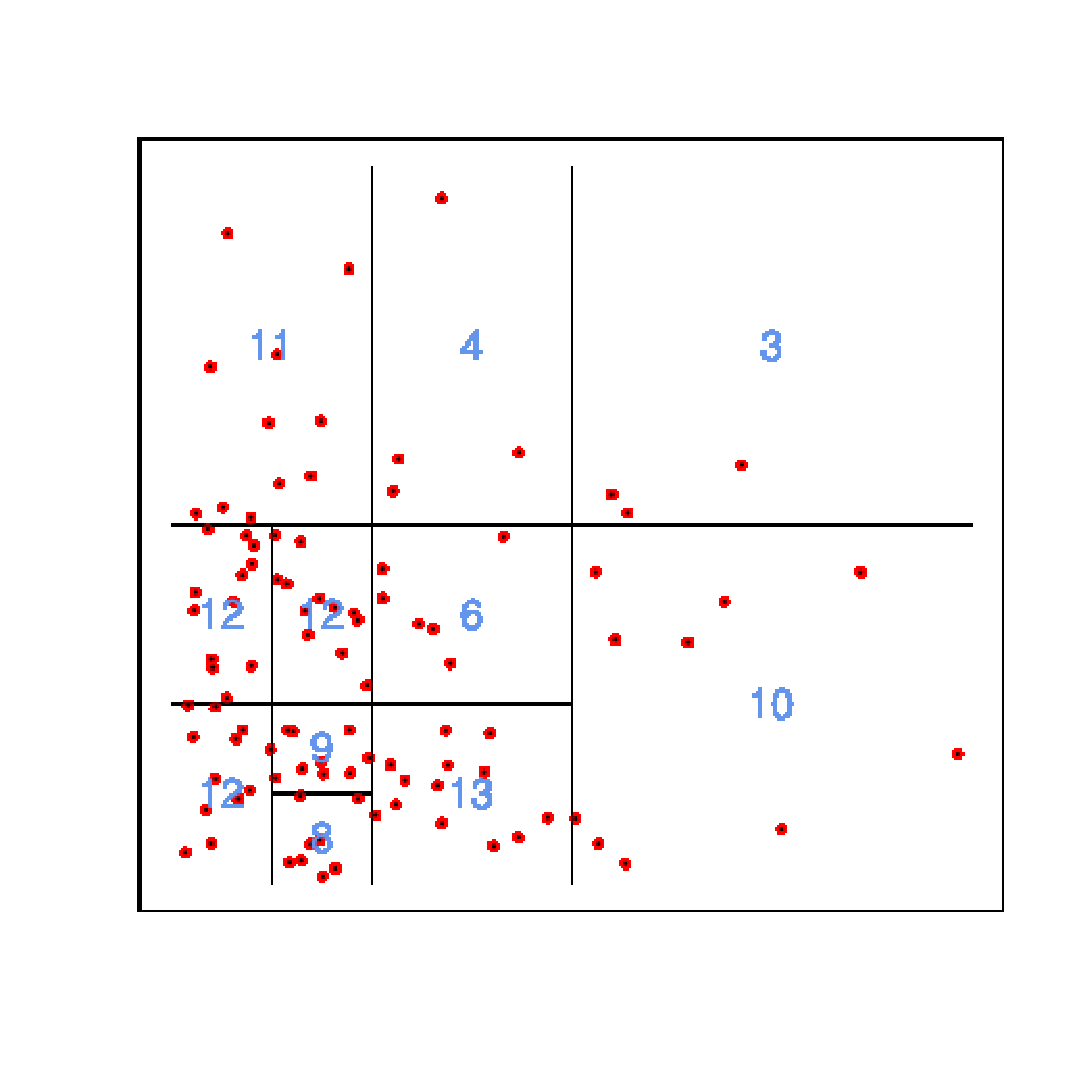
\includegraphics[width=0.3\textwidth]{norm_geom.eps}
	}
	\hspace{3pt}%
	\subfloat[][Cardinal Split]{%
		\label{norm:card}%
		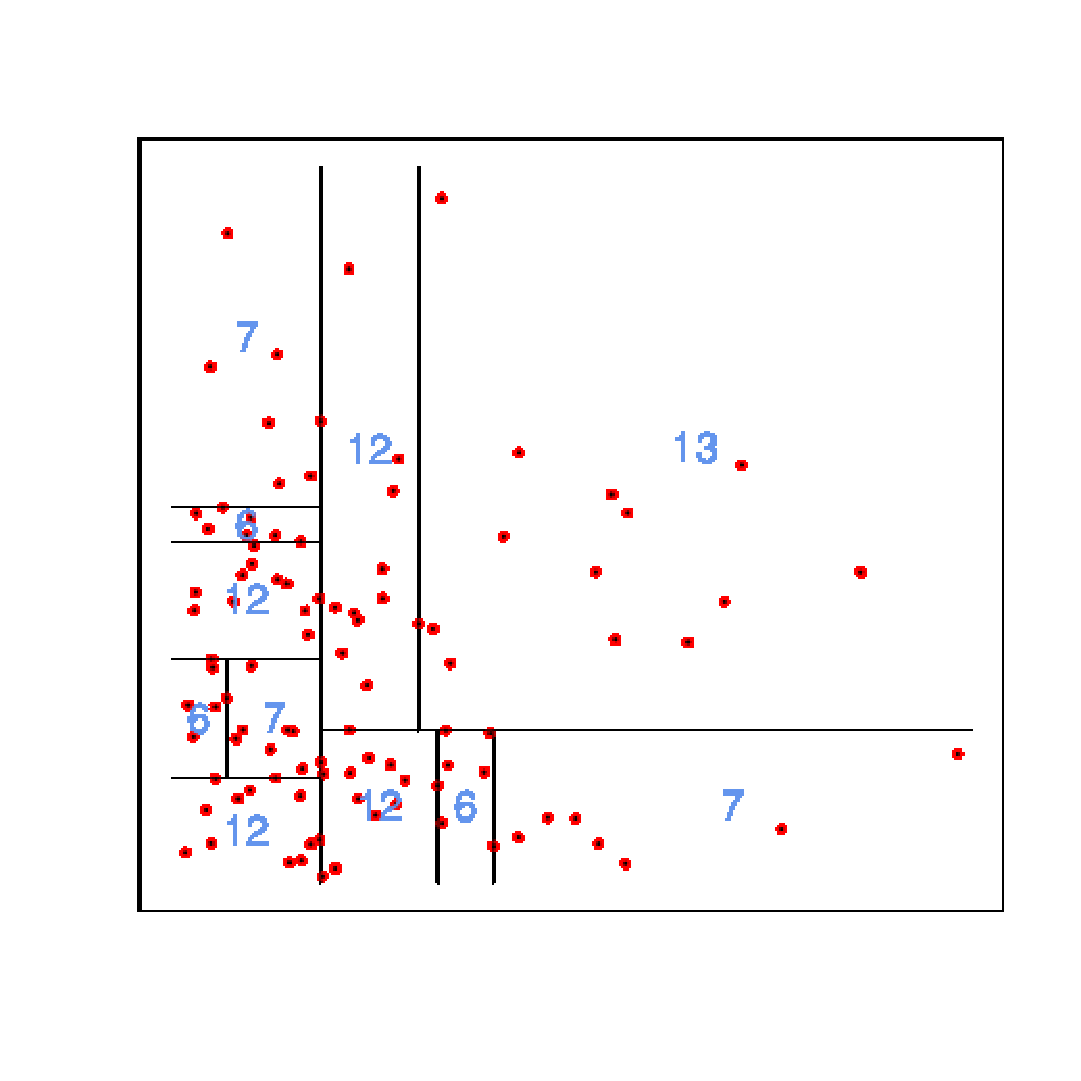
\includegraphics[width=0.3\textwidth]{norm_card.eps}
	}
	\hspace{3pt}%
	\subfloat[][Mean Split]{%
		\label{norm:mean}%
		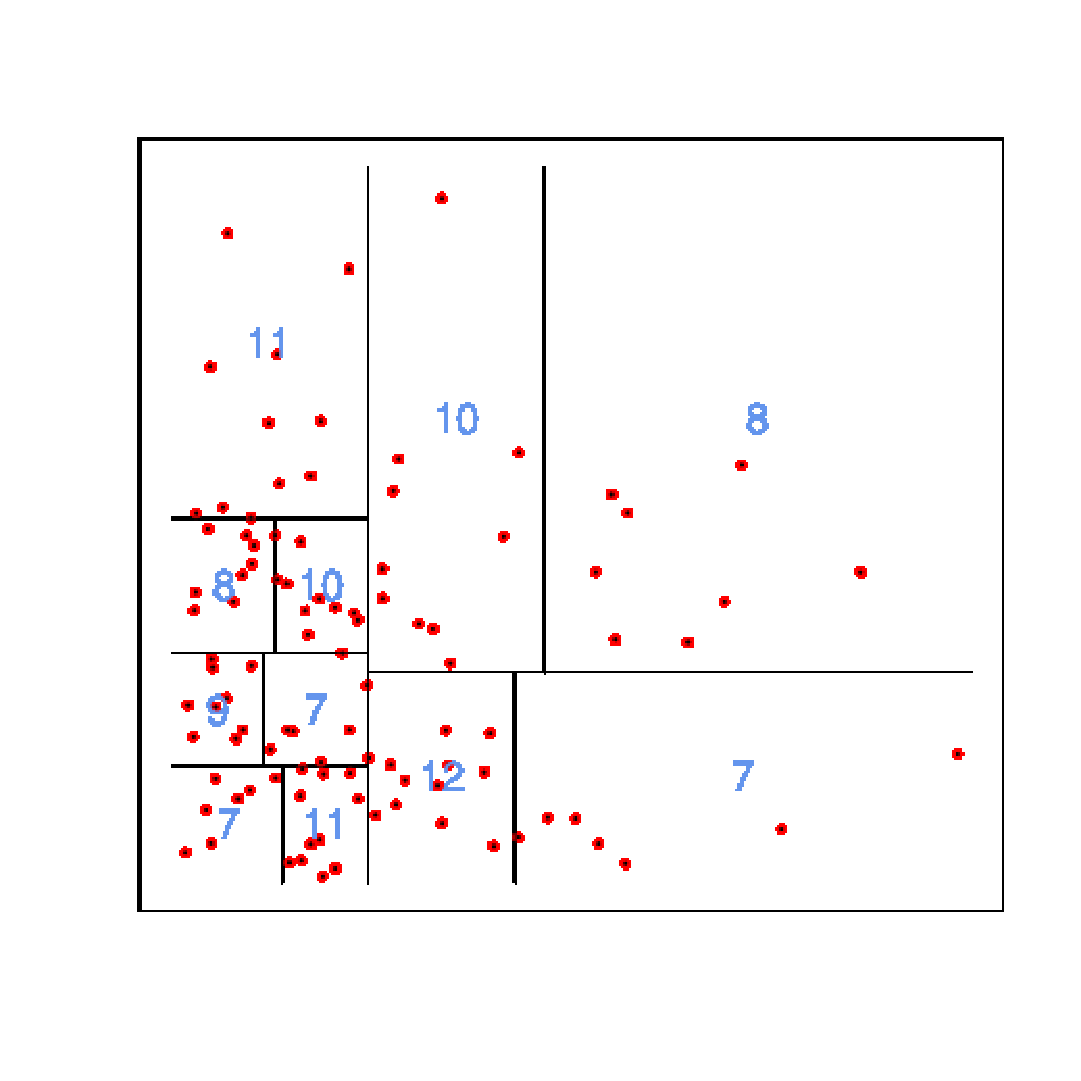
\includegraphics[width=0.3\textwidth]{norm_mean.eps}
	}
	\caption[]{Split domain of point normally distributed $\mathcal{N}\left(0,0.35\right)$}%
	\label{split:norm}
\end{figure}

\begin{figure}
	\centering
	\subfloat[][Geometrical Split]{
		\label{unif:geom}
		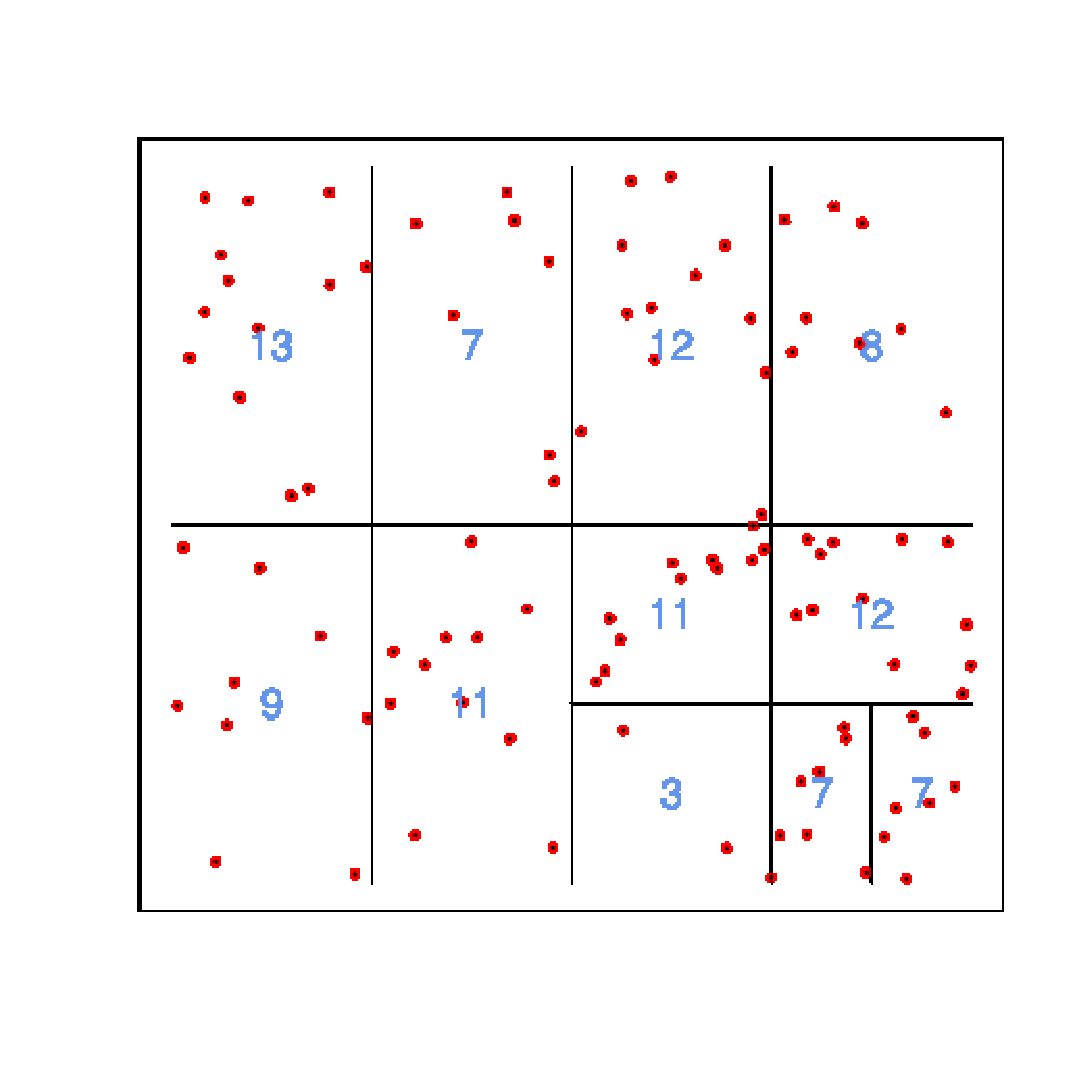
\includegraphics[width=0.3\textwidth]{unif_geom.eps}
	}
	\hspace{3pt}%
	\subfloat[][Cardinal Split]{%
		\label{unif:card}%
		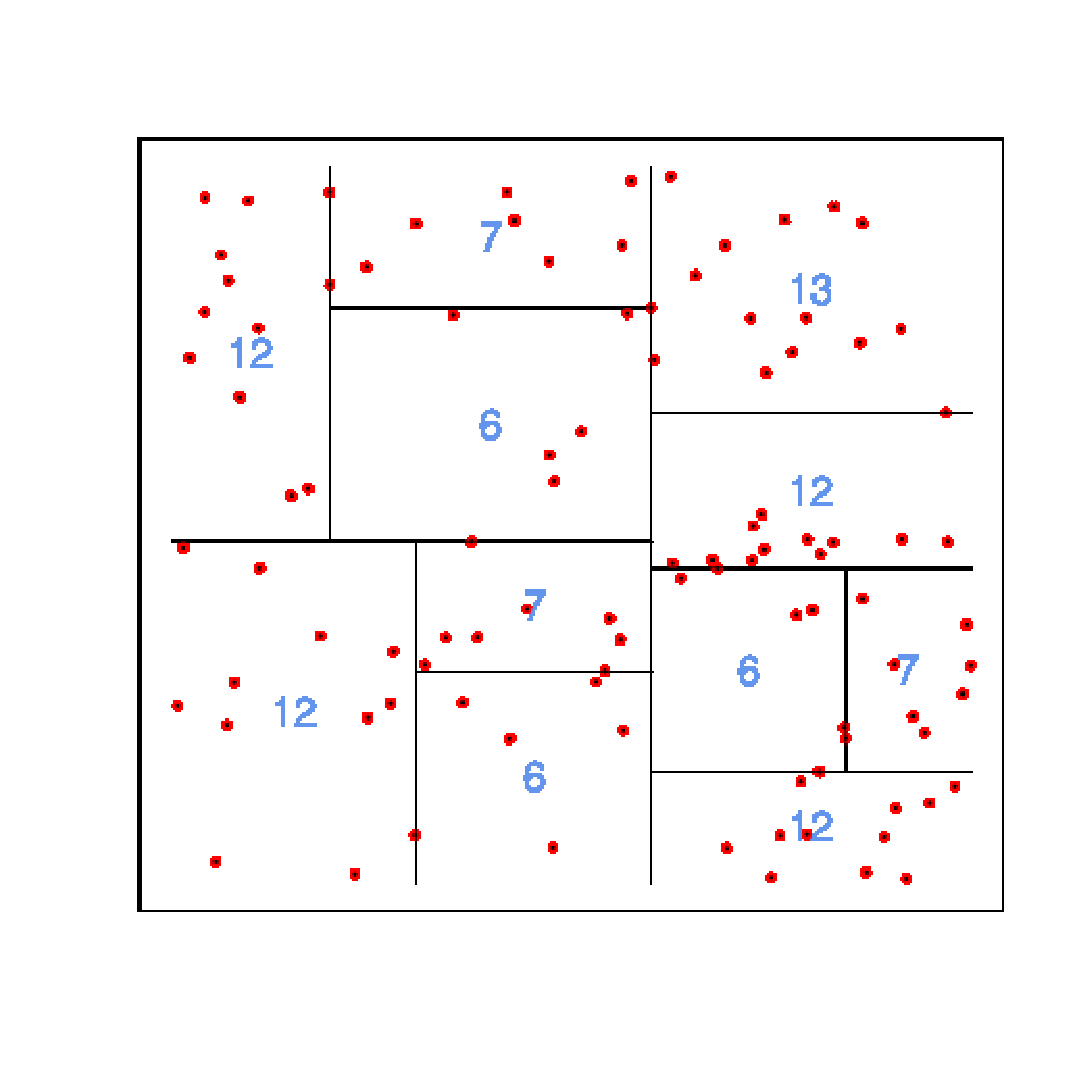
\includegraphics[width=0.3\textwidth]{unif_card.eps}
	}
	\hspace{3pt}%
	\subfloat[][Mean Split]{%
		\label{unif:mean}%
		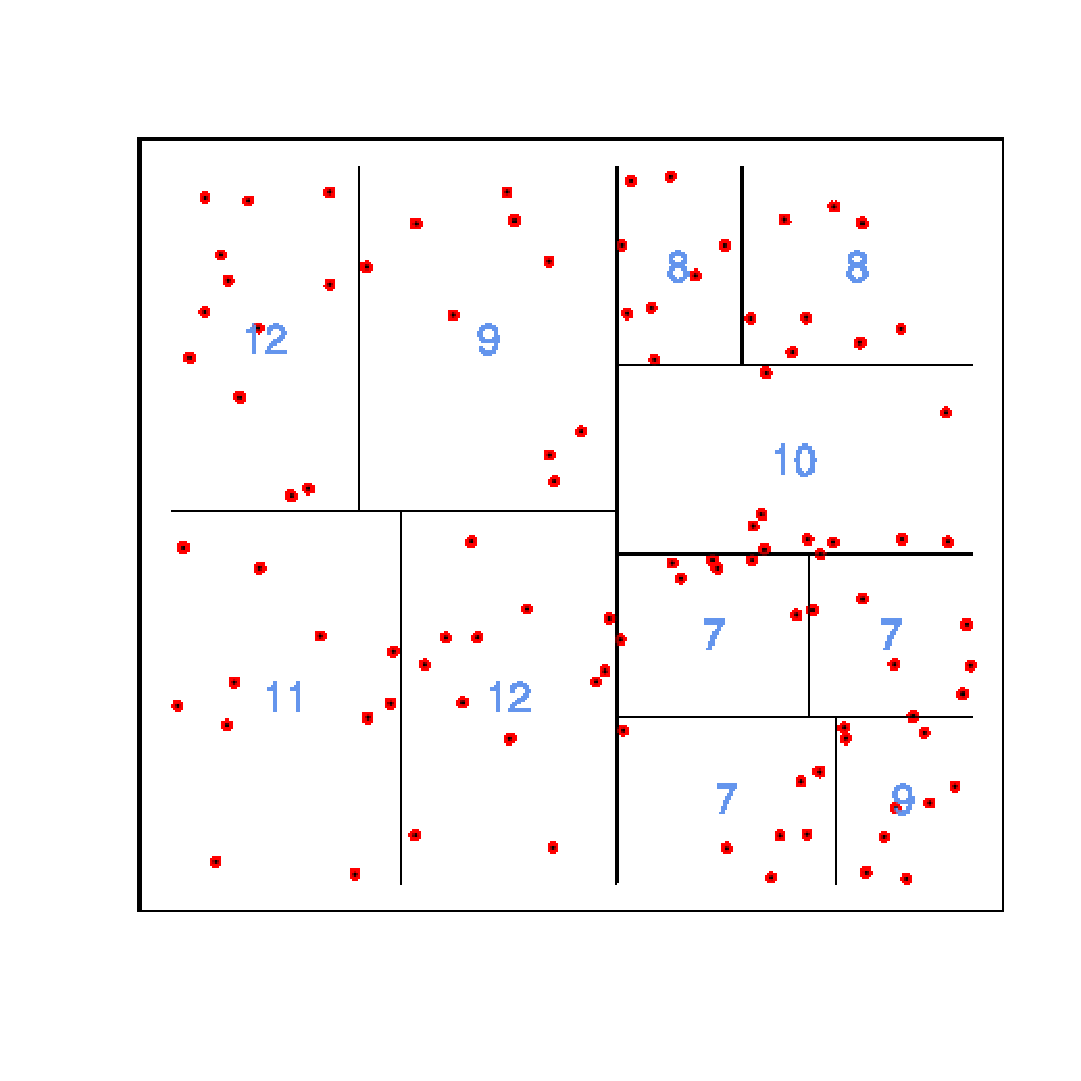
\includegraphics[width=0.3\textwidth]{unif_mean.eps}
	}
	\caption[]{Split domain of point uniformly distributed}%
	\label{split:unif}
\end{figure}

\begin{figure}
	\centering
	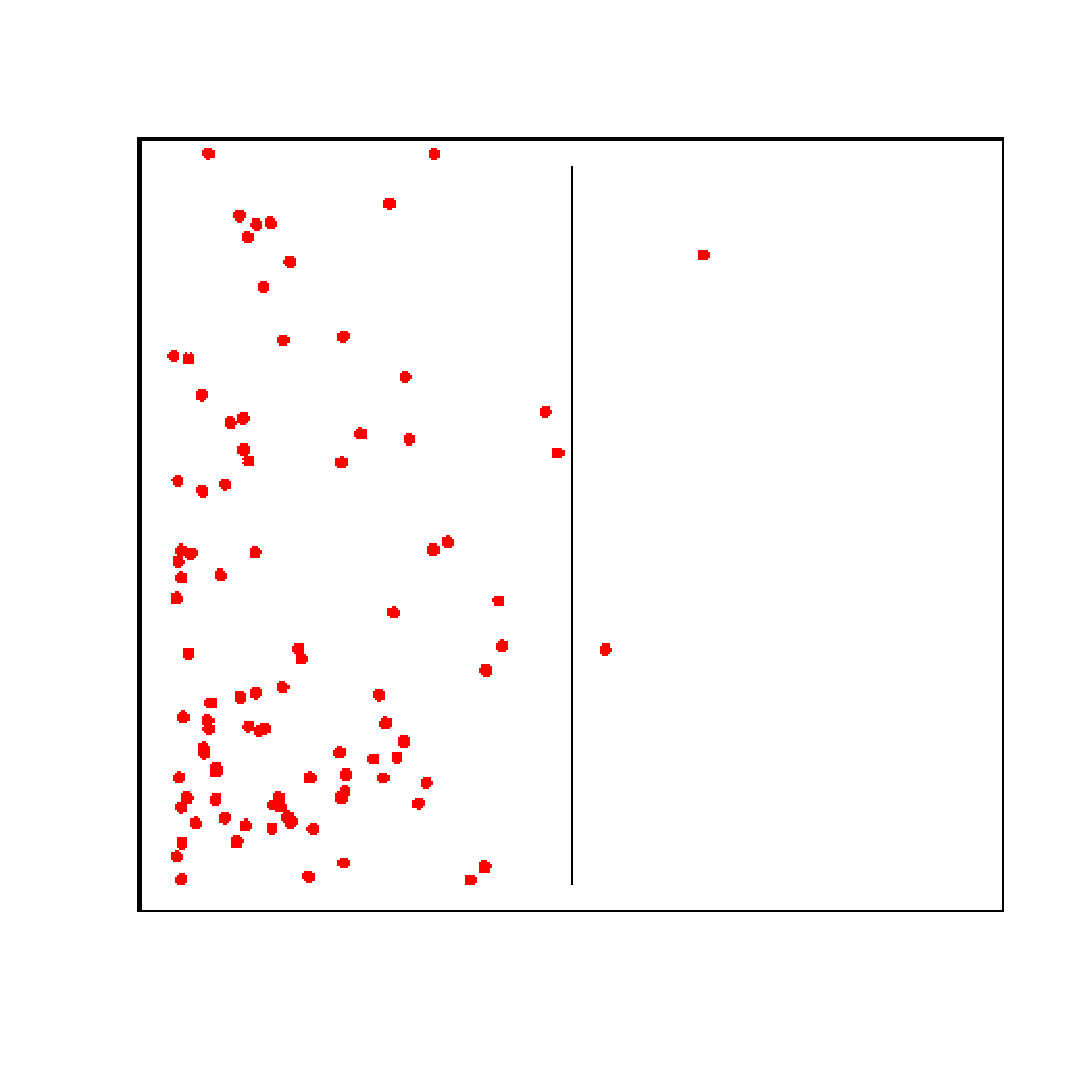
\includegraphics[width=0.3\textwidth]{badGeo.eps}
	\caption[]{If we assume $C = 3$ then this set can't be divided}%
	\label{fig:badGeom}
\end{figure}

\begin{enumerate}
\item {\bf Geometrical Split}: 
\begin{itemize}
\item \underline{Split criterion}: {\it Geometrical} $\rightarrow$ Dividing the region in tow parts with the same area.
\item \underline{Cut point}: The middle point of the x--axis (or y--axis, depending on the shape)
\item \underline{Result}: Two equal regions, but with different amount of clients (see Figure~\ref{norm:geom}). In the next step, the next sub-domain to divide will be, from those already divided, the most populated one (the sub-domain with more clients).
\item \underline{Problem}: Maybe we need to divide a sub-domain because it has a lot of client, but in the other hand it generate a sub-domain with a few clients, as you can see in the Figure~\ref{fig:badGeom}.
\item \underline{Benefit}: Very fast split. If we attack scenarios with point uniformly distributed, the behavior is pretty much desirable, as we can see in the Figure ~\ref{unif:geom}. 
\end{itemize}

\item {\bf Cardinal Split}
\begin{itemize}
\item \underline{Split criterion}: The number of clients, i.e., a sub-domain is divided in such a way that in the resulting sub-sub-domains there will be the same number of clients.
\item \underline{Cut point}: The current sub-domain is ordered and the x--axis (or y--axis, depending on the shape) of the element (location of the client) right in the center is selected to be the {\it cut point}
\item \underline{Result}: Two regions with the same ($\pm 1$) amount of clients (see Figure~\ref{norm:geom}). In the next step, the next sub-domain to divide will be, from those already divided, the most populated one (the sub-domain with more clients).
\item \underline{Problem}: The subdivision process is a bit more costly: we need to group the clients on both sides of a {\it perfect pivot}\footnote{Element of a set with the same number of elements lower and greater than him}.
\item \underline{Benefit}: It guarantees the same cardinality in both new sub-sub-domains.
\end{itemize}

\item {\bf Mean Split}
\begin{itemize}
\item \underline{Split criterion}: This is a mid-point strategy between the two previous. The goal is to find a {\it cut point} to group the elements of the current sub-domain, but in a easy way (fast), for that reason we do not compute the exact middle point to produce two sub-sub-domains with the same cardinality, as in the previous approach, instead of that we work with his expected value: the arithmetic mean.
\item \underline{Cut point}: We compute the mean of the $x$--axis (or $y$--axis) of the elements (locations) of the current sub-domain, and it will be the {\it cut point}
\item \underline{Result}: Two regions with not exact information about their sizes or their cardinality.
\item \underline{Problem}: {\it Idem.}
\item \underline{Benefit}: The {\it cut point} can be obtained by a $O(n)$ number of operations. As we can see in the preliminary results\footnote{The experiments are coded in R\cite{Paradis2005}.} (Figures~\ref{fig:goodMeanNorm} and \ref{fig:goodMeanUnif}), the behavior of this technique is near to the {\it cardinal split} technique, at least for normally and uniformly distributed sets of point.
\end{itemize}
\end{enumerate}

\begin{figure}
	\centering
	\subfloat[][Normally distributed]{
		\label{fig:goodCardNorm}
		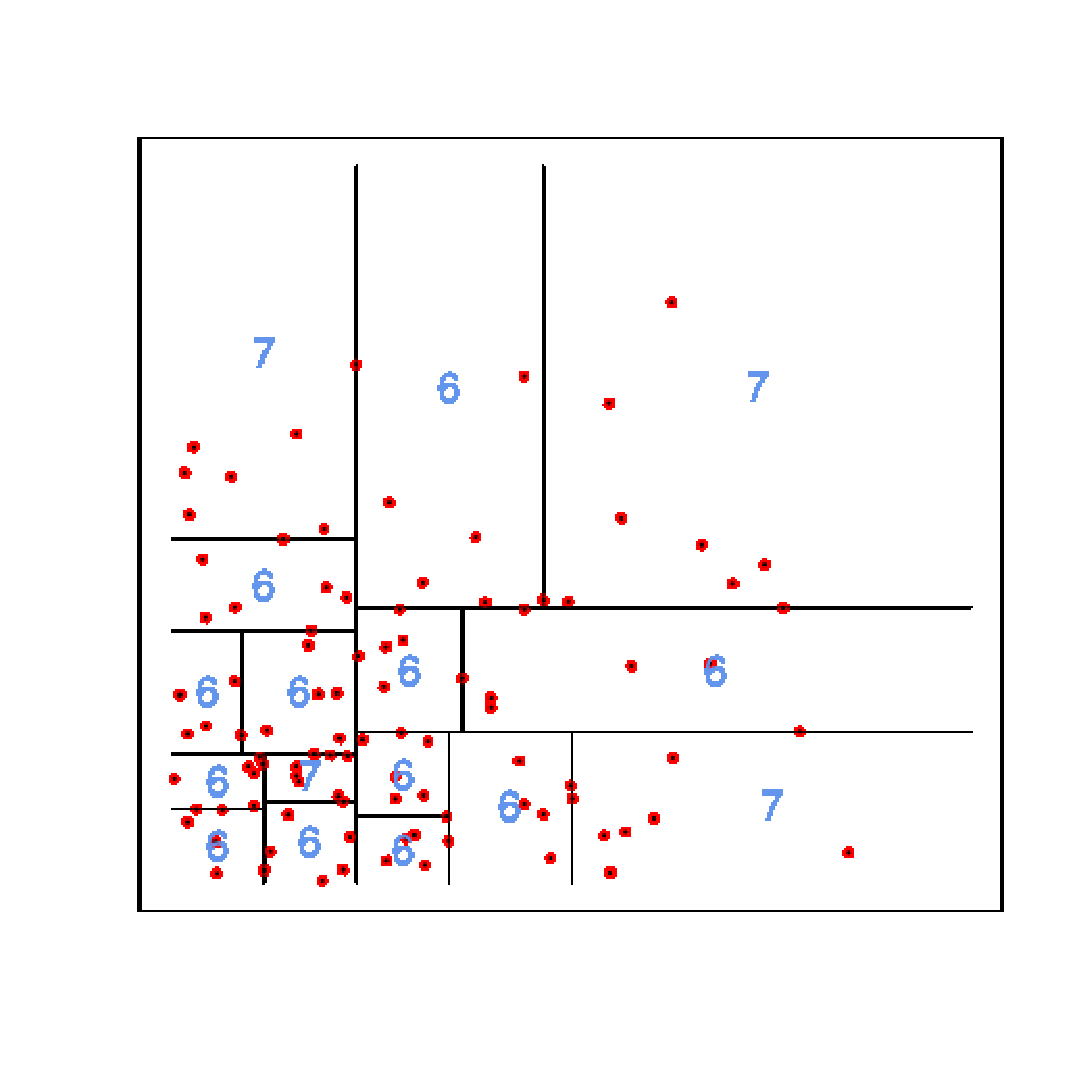
\includegraphics[width=0.3\textwidth]{goodCard.eps}
	}
	\hspace{3pt}%
	\subfloat[][Uniformly distributed]{%
		\label{fig:goodCardUnif}
		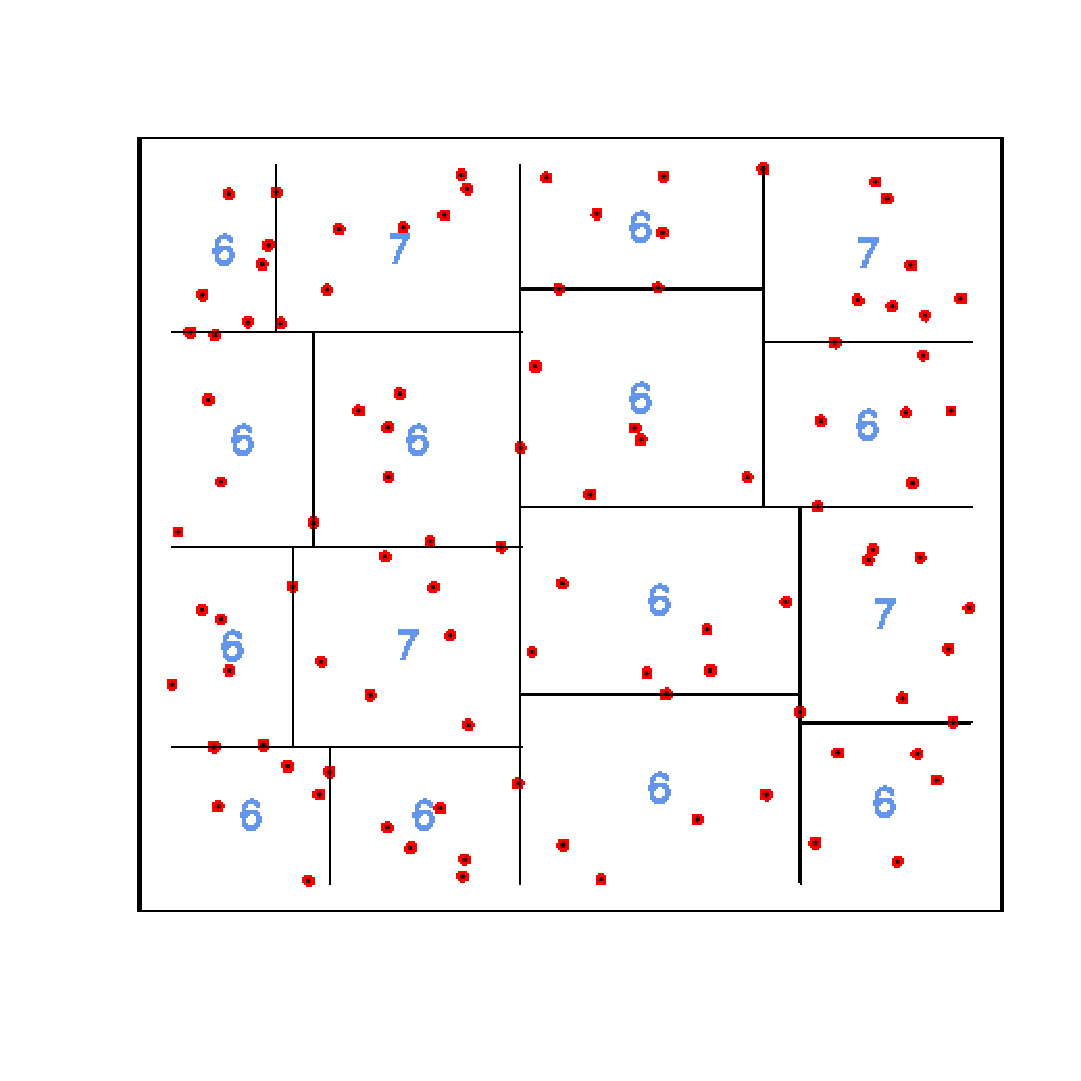
\includegraphics[width=0.3\textwidth]{goodCard2.eps}
	}\\
	\subfloat[][Normally distributed]{
		\label{fig:goodMeanNorm}
		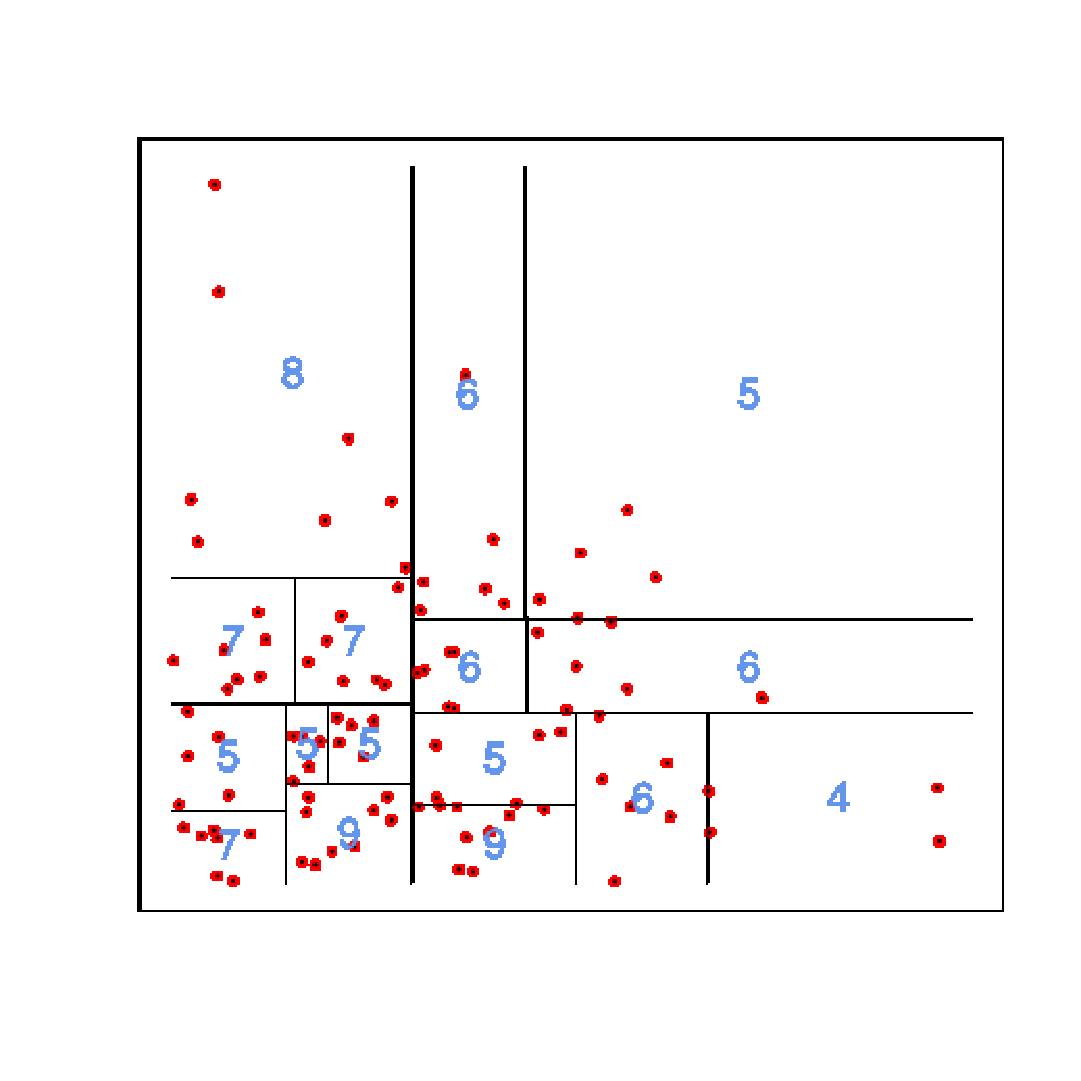
\includegraphics[width=0.3\textwidth]{goodMean.eps}
	}
	\hspace{3pt}%
	\subfloat[][Uniformly distributed]{%
		\label{fig:goodMeanUnif}
		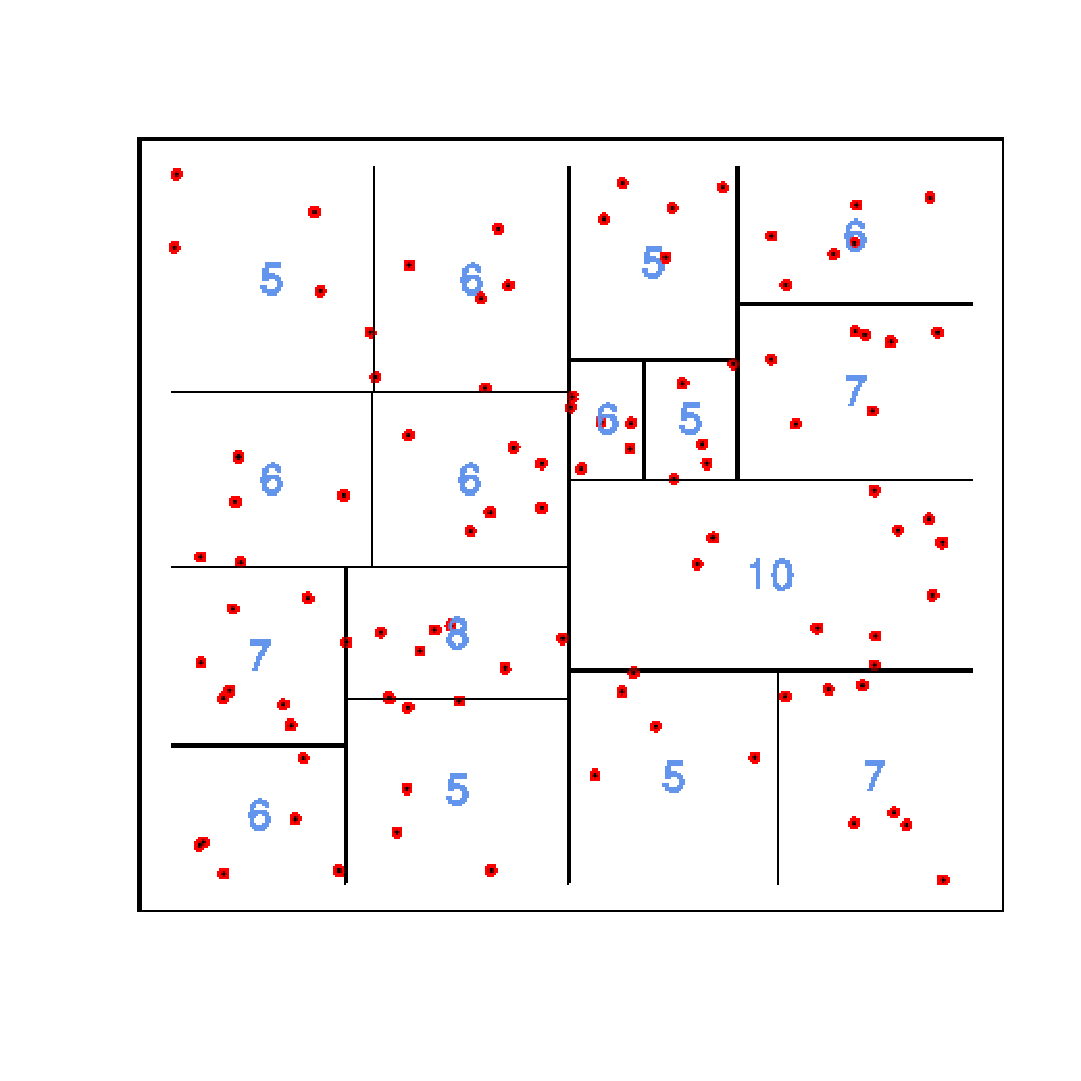
\includegraphics[width=0.3\textwidth]{goodMean2.eps}
	}
	\caption[]{Domain divided in $2^4 = 16$ sub-domains:
		\subref{fig:goodCardNorm} -
		\subref{fig:goodCardUnif} Cardinal;
		\subref{fig:goodMeanNorm} -	
		\subref{fig:goodMeanUnif} Mean.}%
	\label{fig:goodCard}
\end{figure}

%\textcolor{orange}{
%Is easy to see that this strategy guarantees that every built subset has at most two times the elements of some other. Let's take a look to the following example, but first we need to remember that: }
%
%\begin{itemize}
%\item \textcolor{orange}{The point is that every time we choose the most populated set to be divided}
%\item \textcolor{orange}{The current sub-domain is divided in two sub-sub-domains with the same cardinality.}
%\end{itemize} 
%
%\begin{example}
%\textcolor{orange}{
%This example will allow us to intuitively prove the above affirmation.}
%
%\textcolor{orange}{Suppose that there is a sub-domain $A$ in the list with more than two-times the number of element of some other and let's call it $B$. In other words:}
%
%$$\left| A\right| = 2\cdot k\cdot\left| B\right|$$
%$$\text{with } k \in \mathbb{Z}^+$$
%
%\textcolor{orange}{In that case, $B$ was built splitting some other with $\left(2\cdot (k-1)\cdot\left| B\right|\right)$ elements, and it was selected to be divided instead of $A$: \sc{Contradiction!!}}
%\end{example}
%
%\textcolor{orange}{This problem can be avoided forcing the algorithm to generate a quantity of sub-domains power of 2 (see Figure \ref{fig:goodCard}).}

\subsection{Conclusion}

In this section we present a theoretical and not validated work where we applied the {\it search space subdivision} approach to solve {\it k-medoids problem} in parallel. We have proposed some different strategies and we have showed graphically some characteristics of them. 

\section{Tunning methods for local search algorithms}
\label{sec:paramils}


%\textcolor{green}{
%My idea here is to present the work with ParamILS. I worked with the sets of training and test instances, and I think that the key is there, because I obtained a little change in the parameters configuration. The other point is that maybe Costas Array is not a good example to work, because the difference between the runs are too small. I hope that working with other problems, including more training instances, we can obtain better results.}

% short paragraph: about autotuning of parameters; work in progress.

In this section we present our results applying {\sc ParamILS} (version 2.3)\footnote{Open source program (project) in {\it Ruby}, available at \href{http://cs.ubc.ca/labs/beta/Projects/ParamILS}{\texttt{http://cs.ubc.ca/labs/beta/Projects/ParamILS}}}. {\sc ParamILS} (first introduced by Hutter, Hoos and St\:utzle in 2007), is a stochastic local search approach for automated algorithm configuration. The source is available on internet and includes some examples that you can run and see how the tool works. In addition, it brings a complete User Guide with a compact explanation about how to use it with a specific solver \cite{Hutter2008,Hutter2009}. In this study we used it to tune {\it Adaptive Search} solver\footnote{An implementation from Daniel D\'{i}az available at \href{https://sourceforge.net/projects/adaptivesearch/}{https://sourceforge.net/projects/adaptivesearch/}}. %It is an open source program (project) in {\it Ruby}, and the public source code include some examples and a detailed and complete \textit{User Guide} with a compact explanation about how to use it with a specific solver . 

The first step was building a {\it wrapper} in C++ language, in order to tune more than one problem with the same code. The goal of doing this is using the tool to tune the solver, i.e., finding the best parameter configuration for a specific problem, but also the best parameter configuration to solve any kind of benchmark (a general parameter configuration).

\nocite{Rickard}

Following we present in Table~\ref{table:param} the parameter list that we worked with:

\begin{table}[ht] 
\caption{Adaptive Search parameters}
\centering 
\begin{tabular}{c c l}
\hline\hline
Parameter & Type & Description \\ [0.5ex]
\hline
-P & PERCENT & probability to select a local min (instead of staying on a plateau) \\
-f & NUMBER & freeze variables of local min for NUMBER swaps \\ 
-F & NUMBER & freeze variables swapped for NUMBER swaps \\ 
-l & LIMIT & reset some variables when LIMIT variable are frozen \\ 
-p & PERCENT & reset PERCENT of variables \\ [1ex]
\hline
\end{tabular} 
\label{table:param}
\end{table} 

In this section, we explain in details the implementation and the experimentation process.

\subsection{Using ParamILS}

To use the tool {\sc ParamILS}, we have installed Ruby! 1.8.7 in our computer. We used a laptop \mylaptopName (\mylaptopProc, \mylaptopMemo) with {\sc Ubuntu~14.4}. To run the tool, we needed to use the following command line:

\begin{BGVerbatim}
>> ruby param_ils_2_3_run.rb -numRun 0 -scenariofile /.../<scenario_file> -validN 100
\end{BGVerbatim}

Where \texttt{$<$scenario\_file$>$} is the name of the file where we have to put all the information that {\sc ParamILS} needs to tune the solver (the \textit{tuning scenario file}). We explain its content in the next section.

\subsection{Tuning scenario files}

The {\it tuning scenario file} is a text file with all needed information to tune the solver using {\sc ParamILS}. It includes where to find the solver binary file, the parameters domains, etc. In our case, the {\it tuning scenario file} looks like the following:

\begin{shadedbox}
	\texttt{algo = ./QtWrapper\_wrapper\\
		execdir = /.../src \\
		deterministic = 0 \\
		run\_obj = runtime \\
		overall\_obj = mean \\
		cutoff\_time = 50.0 \\
		cutoff\_length = max \\
		tunerTimeout = 3600 \\
		paramfile = instances/all\_intervals-params.txt \\
		outdir = instances/all\_intervals-paramils-out \\
		instance\_file = instances/.../all\_intervals-lower-instances.txt \\
		test\_instance\_file = instances/.../all\_intervals-upper-instances.txt \\
	}
\end{shadedbox}

We explain in details each line in this file:

\begin{itemize}
	\item \textbf{\texttt{algo}} $\rightarrow$ An algorithm executable or a call to a wrapper script around an algorithm that aims the input/output format of \textit{ParamILS} (the wrapper).
	\item \textbf{\texttt{execdir}} $\rightarrow$ Directory to execute \textbf{\texttt{algo}} from: "cd $<$\texttt{execdir}$>$; $<$\texttt{algo}$>$" 
	\item \textbf{\texttt{run\_obj}} $\rightarrow$ A scalar quantifying how "good" a single algorithm execution is, such as its required runtime.
	\item \textbf{\texttt{overall\_obj}} $\rightarrow$ While \textbf{\texttt{run\_obj}} defines the objective function for a single algorithm run, \textbf{\texttt{overall\_obj}} defines how those single objectives are combined to reach a single scalar value to compare two parameter configurations. Implemented examples include {\bf mean}, {\bf median}, {\bf q90} (the 90\% quantile), {\bf adj\_mean} (a version of the mean accounting for unsuccessful runs: total runtime divided by number of successful runs), {\bf mean1000} (another version of the mean accounting for unsuccessful runs: (total runtime of successful runs + 1000 x runtime of unsuccessful runs) divided by number of runs -- this effectively maximizes the number of successful runs, breaking ties by the runtime of successful runs; it is the criterion used in most of Frank experiments), and {\bf geomean} (geometric mean, primarily used in combination with \textbf{\texttt{run\_obj}} = \texttt{speedup}. The empirical statistic of the cost distribution (across multiple instances and seeds) to be minimized, such as the mean (of the single run objectives). \footnote{We use {\bf mean} but maybe we can experiment with other values}
	\item \textbf{\texttt{cutoff\_time}} $\rightarrow$ The time after which a single algorithm execution will be terminated unsuccessfully. This is an important parameter: if chosen too high, lots of time will be wasted with unsuccessful runs. If chosen too low the optimization is biased to perform well on easy instances only.
	\item \textbf{\texttt{tunerTimeout}} $\rightarrow$ The timeout of the tuner. Validation of the final best found parameter configuration starts after the timeout.
	\item \textbf{\texttt{paramfile}} $\rightarrow$ Specifies the file with the parameters of the algorithms. 
	\item \textbf{\texttt{outdir}} $\rightarrow$ Specifies the directory \textit{ParamILS} should write its results to.
	\item \textbf{\texttt{instance\_file}} $\rightarrow$ Specifies the file with a list of training instances. 
	\item \textbf{\texttt{test\_instance\_file}} $\rightarrow$ Specifies the file with a list of test instances.
\end{itemize}

Another important file that we have to compose properly is the {\it algorithm parameter file}, just following the instruction from \cite{Hutter2008} --\textit{[...] each line lists one parameter, in curly parentheses the possible values considered, and in square parentheses the default value [...]}. Our {\it algorithm parameter file} looks like follows:\\

\begin{shadedbox}
	\texttt{P \{20, 25, 30, 35, 40, 45, 50, 55, 60\} [50]\\
		f \{0, 1, 2, 3\} [1]\\
		F \{0, 1, 2, 3\} [0]\\
		l \{0, 1, 2, 3\} [1]\\
		p \{1, 2, 3, 5, 10, 20\} [5]
	}
\end{shadedbox}

In the current {\it Adaptive Search} implementation, the solver binary file and the problem instance are the same thing. It means that we only have to use the following command to solve the {\it All--intervals} problem of size $K$, for example: 

\begin{BGVerbatim}
>> ./all-intervals K
\end{BGVerbatim}

So, to use {\sc ParamILS} we modified a little the code: now our solver takes the size parameter from a text file. That way, the instance file is a text file only containing a number.

The solver we want to tune using {\sc ParamILS} ({\it Adaptive Search} in this case), must aims specific input/output rules. For that reason instead of modifying the current code of {\it Adaptive Search} implementation, we preferred to build a wrapper.

\subsection{Building the wrapper}

The algorithm executable must follow the input/output criteria presented below: 

\textbf{\large Launch command:} 

\begin{BGVerbatim}
>> <algo_exectuable> <instance_name> <instance-specific_information> ...
<cutoff_time> <cutoff_length> <seed> <params>
\end{BGVerbatim}

\begin{itemize}
	\item \texttt{$<$algo\_exectuable$>$} Solver 
	\item \texttt{$<$instance\_name$>$} In our case, a text file containing only the problem size
	\item \texttt{$<$instance-specific\_information$>$} We don't use it 
	\item \texttt{$<$cutoff\_time$>$} Cut off time for each run of the solver (see above)
	\item \texttt{$<$cutoff\_length$>$} We don't use it
	\item \texttt{$<$seed$>$} Random seed
	\item \texttt{$<$params$>$} Parameters and its values
\end{itemize}

\underline{Exmaple:}

\begin{BGVerbatim}
>> ./QtWrapper_320.txt "" 50.0 214483647 524453158 -p 5 -l 1 -f 1 -P 50 -F 0
\end{BGVerbatim}

\textbf{\large Output:} 

\begin{BGVerbatim}
>> <solved>, <runtime>, <runlength>, <best_sol>, <seed>
\end{BGVerbatim}

\begin{itemize}
	\item {\bf $<$solved$>$} \texttt{SAT} if the algorithm terminates successfully. \texttt{TIMESOUT} if the algorithm times out.
	\item {\bf $<$runtime$>$} Runtime
	\item {\bf $<$runlength$>$} -1 (as Frank Hutter recommended)
	\item {\bf $<$best\_sol$>$} -1 (as Frank Hutter recommended)
	\item {\bf $<$cutoff\_length$>$} We don't use it
	\item {\bf $<$seed$>$} Used random seed
\end{itemize}

\underline{Exmaple:}

\begin{BGVerbatim}
>> SAT, 2.03435, -1, -1, 524453158
\end{BGVerbatim}

To build the wrapper we have followed a simple algorithm: launch two concurrent process. In the parent process we translate the input of the wrapper to the input of {\it Adaptive Search} solver. The solver is executed, and the runtime is measured. After that we post the output properly. In the child process a {\it sleep} command is executed for \texttt{$<$runtime$>$} seconds and after that, if the parent process has not finished yet, it is killed, posting a time-out message. See Algorithm~\ref{wrapper} for more details.

%\incmargin{1.4em}
\linesnumbered
\begin{algorithm}[H]
	\caption{Costas Wrapper}
	\label{wrapper}
	\dontprintsemicolon
	\SetLine
	\SetKwData{paramConfig}{$\theta$}
	\SetKwData{seed}{s}
	\SetKwData{Inst}{$Pth_{\pi}$}
	\SetKwData{cotime}{$k$}
	\SetKwData{pilsOut}{$PiLS_{out}$}
	\SetKwData{tstart}{$t_0$}
	\SetKwData{tend}{$t_e$}
	\SetKwData{timet}{$t$}
	\SetKwData{strCal}{strCall}
	\SetKwFunction{fork}{fork}
	\SetKwFunction{TIC}{clock\_TIC}
	\SetKwFunction{TOC}{clock\_TOC}
	\SetKwFunction{buildStr}{build\_str}
	\SetKwFunction{call}{systemCall}
	\SetKwFunction{kill}{killProcess}
	\SetKwFunction{output}{paramilsOutput}
	\SetKwFunction{sleep}{sleep}
	\SetKwInOut{Input}{input}
	\SetKwInOut{Output}{output}
	
	\Input{\Inst : problem instance path, \cotime : cut off time, \seed : random seed, \paramConfig : parameters configuration}
	\Output{\pilsOut : Output in a {\sc ParamILS} way}
	\BlankLine
	
	\fork{} \tcc{Divide the execution in two processes}
	\eIf{$<$in child process$>$}{
		\tstart $\leftarrow$ \TIC{}\;
		\strCal $\leftarrow$ \buildStr{\texttt{" ./AS\_Wrapper \%1 -s \%2 \%3"}, \Inst, \seed, \paramConfig}\;
		\call{\strCal}\;
		\tend $\leftarrow$ \TOC{}\;
		\kill{$<$parent process$>$} \label{paso7}\;
		\timet $\leftarrow$ \tend - \tstart\;
		{\bf return} \output{SAT, \timet, \seed}\;
	}{
	\sleep{\cotime}\;
	\kill{$<$child process$>$}\;
	{\bf return} \output{TIMESOUT, \cotime, \seed}\;
}
\end{algorithm}

\subsection{Using the wrapper}

In this section we explain how to use our wrapper to be able to tune easily instances of {\it All-Interval Series} and \carr{} problems. The {\it All-Interval Series Problem}\footnote{CSPlib:007 (\href{http://www.csplib.org/Problems/prob007/}{\texttt{http://www.csplib.org/Problems/prob007/}})} is the problem of finding a vector $s=\left(s_1,\dots,s_n\right)$, given $n \in \mathbb{N}$, such that $s$ is a permutation of the vector $(0, 1, \dots, n-1)$ and the interval vector $v = \left(\left|S_2-s_1\right|, \left|S_3-s_2\right|, \dots, \left|S_n-S_{n-1}\right|\right)$ (called an all-interval series of size $n$) is a permutation of the vector $(1, 2, \dots, n-1)$. The \carrp{} consists in finding a Costas array, which is an $n\times n$ grid containing $n$ marks such that there is exactly one mark per row and per column and the $n(n-1)/2$ vectors joining each couple of marks are all different (see below for more details about this problems).

\subsubsection{Factory call}

The first step is to implement the class {\sc ICallFactory}. Here, the string-binary-name for the command call is statically obtained. We present, as example, the class {\sc All\_IntervalCallFactory}:

\begin{Verbatim}[fontsize=\normalsize]
\textcolor{verde}{\bf// all_interval_call_factory.h}
\textcolor{blue}{\bf class} All_IntervalCallFactory: \textcolor{blue}{\bf public} ICallFactory
\{
   \textcolor{blue}{\bf public}:
      std::string BuildCall();
      std::string BuildDefaultCall();
\};
\end{Verbatim}

\begin{Verbatim}[fontsize=\normalsize]
\textcolor{verde}{\bf// all_interval_call_factory.cpp}
\textcolor{dred}{\bf #define} ALGO_EXECUTABLE "./all-interval"
\textcolor{dred}{\bf #define} DEFAULT_CALL "./all-interval _100.txt"

std::string All_IntervalCallFactory::BuildCall()
\{
   \textcolor{blue}{\bf return} ALGO_EXECUTABLE;
\}
std::string All_IntervalCallFactory::BuildDefaultCall()
\{
   \textcolor{blue}{\bf return} DEFAULT_CALL;
\}
\end{Verbatim}

All we have to do is to define our new macro {\bf ALGO\_EXECUTABLE} ({\bf DEFAULT\_CALL} is not being used)

\subsubsection{Main method}

Let's suppose now that we want to run an algorithm called {\it mySolver} that receives a file as parameter, called {\it my\_instance\_size.txt} (this is mandatory). We have to create (as we've explained before) the class {\sc My\_SolverCallFactory} and defining the macro as follows:

\begin{Verbatim}[fontsize=\normalsize]
\textcolor{dred}{\bf #define} ALGO_EXECUTABLE "./mySolver"
\end{Verbatim}

Now, the main method would be exactly like this:

\begin{Verbatim}[fontsize=\normalsize]
\textcolor{blue}{\bf int} main(\textcolor{blue}{\bf int} argc, \textcolor{blue}{\bf char}* argv[])
\{
   shared_ptr<ICallFactory> problem = 
      make_shared<My_SolverCallFactory>();
   shared_ptr<TuningData> td = 
      (make_shared<TuningData>(argc, argv, problem));

   shared_ptr<ADWrapper> w (make_shared<ADWrapper>());
   string output = w->tune(td);

   cout << output << endl;
   \textcolor{blue}{\bf return} 0;
\}
\end{Verbatim}

\subsection{Results}

In this section we present the results of applying {\sc ParamILS} to the resolution of {\it All-Interval Series} and \carr{} problems through {\it Adaptive Search}. In both cases, we need to chose a set of {\it training instances}, to train the tuner, and a set of {\it test instances}, used to obtain the parameter setting. 

\subsubsection{ Tuning {\it Adaptive Search} for  {\it All-Intervals Series Problem}}

\underline{Study cases:}
\begin{enumerate}
	\item The {\it training instances set} is composed by instances of {\it All--Intervals} problems of order $N$ with $$N \in \left\{100, 110, 120, 130, 140, 150, 160, 170, 180\right\}$$
	\item The {\it test instances set} is composed by instances of {\it All--Intervals} problems of order $N$ with $$N \in \left\{190, 200, 210, 220, 230, 240, 250, 260, 265\right\}$$
	\item The time-out for each run is 50.0 seconds
	\item The test quality is based on 100 runs
\end{enumerate}

In a {\bf First Experiment} we use the following {\it parameters domains}:
\begin{itemize}[itemsep=0.2mm]
	\item {\bf P}\texttt{ \{41, 46, 51, 56, 60, 66, 71, 76, 80\}}
	\item {\bf F, f, l}\texttt{ \{0, 1, 2, 3\}}
	\item {\bf p}\texttt{ \{5, 10, 15, 20, 25, 30, 35\}}
\end{itemize}

Table~\ref{table:allint5yh} shows results using a time-out of 5.5 hours (20,000 seconds), and Table~\ref{table:allint1h} shows results using a time-out of 1 hour. In the second case we where able to perform more runs, due to the available time, but in both cases the training qualities are not so different. However, we can se the difference int the test qualities, and conclude that results using 5 hours of time-out are more reliables. 

\begin{table}[h] 	
\centering 
\renewcommand{\arraystretch}{1.2}
\resizebox{\columnwidth}{!}{%
\tablePILSresults{
	0 & 66 & 1 & 1 & 25 & 0 & 80 & 2 & 1 & 35 & 0.79666 & 1780 & 8.274 \\
	2 & 56 & 2 & 2 & 20 & 1 & 80 & 1 & 1 & 10 & 0.795 & 1637 & 5.508 \\
	0 & 41 & 0 & 0 & 5 & 1 & 80 & 3 & 0 & 15 & 0.789 & 1547 & 5.8478 \\
	3 & 80 & 3 & 3 & 35 & 1 & 80 & 2 & 0 & 10 & 0.880686 & 1258 & 6.15398\\
}
}
\caption{{\it All-Intervals Series}: \texttt{tunerTimeout} = 20,000 seconds}\label{table:allint5yh}
\end{table}

\begin{table}[h] 	
\centering 
\renewcommand{\arraystretch}{1.2}
\resizebox{\columnwidth}{!}{%
\tablePILSresults{
	0 & 66 & 1 & 1 & 25 & 0 & 80 & 0 & 1 & 25 & 0.815 & 384 & 5.8191 \\
	0 & 66 & 1 & 1 & 25 & 1 & 80 & 1 & 1 & 35 & 0.737 & 452 & 6.267 \\
	0 & 66 & 1 & 1 & 25 & 1 & 56 & 0 & 1 & 35 & 1.03 & 371 & 9.056 \\
	0 & 66 & 1 & 1 & 25 & 0 & 76 & 0 & 1 & 20 & 0.814 & 385 & 4.915 \\
	0 & 66 & 1 & 1 & 25 & 0 & 80 & 3 & 1 & 20 & 0.76 & 469 & 5.417 \\ 
	\hline
	2 & 56 & 2 & 2 & 20 & 0 & 41 & 0 & 1 & 10 & 0.919 & 239 & 18.364 \\
	2 & 56 & 2 & 2 & 20 & 0 & 56 & 1 & 1 & 20 & 0.819 & 407 & 5.409 \\
	2 & 56 & 2 & 2 & 20 & 1 & 80 & 1 & 1 & 35 & 0.772 & 457 & 5.43 \\
	2 & 56 & 2 & 2 & 20 & 1 & 80 & 0 & 1 & 10 & 0.858 & 504 & 5.566 \\
	2 & 56 & 2 & 2 & 20 & 0 & 80 & 1 & 1 & 10 & 0.7845 & 562 & 18.944 \\
	\hline
	0 & 41 & 0 & 0 & 5 & 0 & 41 & 1 & 0 & 10 & 0.9749 & 367 & 5.97813 \\
	0 & 41 & 0 & 0 & 5 & 0 & 41 & 1 & 0 & 10 & 0.885 & 450 & 5.706 \\
	0 & 41 & 0 & 0 & 5 & 0 & 41 & 1 & 0 & 10 & 0.906 & 335 & 18.707 \\
	0 & 41 & 0 & 0 & 5 & 0 & 41 & 1 & 0 & 10 & 0.995 & 335 & 19.558 \\
	0 & 41 & 0 & 0 & 5 & 0 & 41 & 0 & 0 & 5 & 0.855 & 404 & 5.686 \\
	\hline
	3 & 80 & 3 & 3 & 35 & 0 & 66 & 3 & 1 & 25 & 0.9118 & 230 & 26.585 \\
	3 & 80 & 3 & 3 & 35 & 0 & 80 & 1 & 1 & 10 & 0.732 & 310 & 7.875 \\
	3 & 80 & 3 & 3 & 35 & 0 & 80 & 0 & 1 & 20 & 0.816 & 303 & 7.2896 \\
	3 & 80 & 3 & 3 & 35 & 1 & 80 & 3 & 1 & 35 & 0.821 & 327 & 6.812 \\
	3 & 80 & 3 & 3 & 35 & 0 & 80 & 0 & 1 & 30 & 0.9203 & 443 & 5.401 \\
} 
}
\caption{{\it All-Intervals Series}: \texttt{tunerTimeout} = 3,600 seconds}\label{table:allint1h}
\end{table}

In a {\bf Second Experiment} we decide to enlarge a bit more the parameters domains and use a time-out of 5 hours. The {\bf Parameters domains} are the following:
\begin{itemize}[itemsep=0.2mm]
	\item {\bf P}\texttt{ \{10, 20, 30, 40, 50, 60, 70, 80, 90\}}
	\item {\bf F, f, l}\texttt{ \{0, 1, 2, 3, 4, 5, 6, 7, 8\}}
	\item {\bf p}\texttt{ \{10, 20, 30, 40, 50, 60, 70\}}
\end{itemize}

\begin{table}[h] 	
\centering 
\renewcommand{\arraystretch}{1.2}
\resizebox{\columnwidth}{!}{%
\tablePILSresults{
	0 & 10 & 0 & 0 & 10 & 0 & 40 & 7 & 0 & 50 & 0.883188 & 936 & 6.3191 \\
	0 & 10 & 0 & 0 & 10 & 0 & 80 & 2 & 1 & 40 & 0.774659 & 1584 & 5.45674 \\ 
	0 & 10 & 0 & 0 & 10 & 0 & 40 & 2 & 0 & 10 & 0.96885 & 1104 & 6.82643 \\ 
	\hline
	4 & 60 & 4 & 4 & 40 & 0 & 60 & 8 & 1 & 40 & 0.90358 & 1566 & 5.48127 \\
	4 & 50 & 4 & 4 & 40 & 0 & 80 & 5 & 1 & 20 & 0.78536 & 1662 & 11.5649 \\
	3 & 50 & 4 & 2 & 30 & 0 & 90 & 6 & 1 & 70 & 0.79440 & 1395 & 5.08108 \\
	\hline
	0 & 90 & 0 & 0 & 10 & 1 & 90 & 6 & 1 & 10 & 0.859569 & 1379 & 5.4286 \\ 
	0 & 90 & 0 & 0 & 10 & 1 & 90 & 6 & 1 & 30 & 0.80738 & 1117 & 5.47126 \\
	8 & 90 & 8 & 8 & 60 & 0 & 80 & 5 & 1 & 10 & 0.834934 & 1384 & 5.5377 \\
	\hline
	5 & 30 & 2 & 3 & 60 & 0 & 90 & 1 & 0 & 20 & 0.862013 & 1707 & 5.21837 \\
	3 & 20 & 2 & 4 & 60 & 0 & 80 & 6 & 1 & 10 & 0.805604 & 1630 & 5.4467 \\ 
	6 & 70 & 1 & 3 & 50 & 0 & 80 & 5 & 1 & 10 & 0.792600 & 1344 & 5.46558 \\  
	6 & 40 & 1 & 3 & 30 & 1 & 80 & 7 & 0 & 20 & 0.822703 & 1977 & 5.41185 \\
} 
}
\caption{{\it All-Intervals Series}: \texttt{tunerTimeout} = 18,000 seconds}\label{table:allint5h}
\end{table}

The results presented in Table~\ref{table:allint5h} show better results in terms of test quality with respect to Table~\ref{table:allint5yh}. For that reason, in the \textbf{FINAL Experiment}, only the results obtained in those tables were took into account (also because they were obtained by using longer times-out). As it can be observed in those tables, {\it Adaptive Search} seems to show a good behavior if the parameters {\bf F}, {\bf P} and {\bf l} are in the following sets: \texttt{\bf F} $\in$ \texttt{\{ 0, 1\}}, \texttt{\bf P} $\in$ \texttt{\{ 80, 90\}} and \texttt{\bf l} $\in$ \texttt{\{ 0, 1\}}.

In that sense, a specific configuration was extracted from the results above, and 60 runs of {\it Adaptive Search} were performed solving {\it All--Intervals} ($N = 600$) benchmark:
\begin{itemize}
	\item[-] 30 using the default parameter configuration (\texttt{-F 0 -P 66 -f 1 -l 1 -p 25})
	\item[-] 30 with an optimal parameter configuration extracted from the Tables~\ref{table:allint5yh}, \ref{table:allint5h} (\texttt{-F 0 -P 80 -f 6 -l 1 -p 10})
\end{itemize}

Table~\ref{table:testaibad} shows results by using the default parameter settings, and Table~\ref{table:testaigood} shows the results by using the parameter configuration found by {\sc ParamILS}, and it is clear that the default configuration shows better results than {\it ParamILS}'s one, in terms both of runtime mean and standard deviation Using the default parameter settings, {\it Adaptive Search} can obtains best results int terms of {\it mean} and {\it slowest run}. However, using the {\sc ParamILS} found parameter settings, it reached a {\it fastest} run two times faster than the one using the default parameter settings. 

\begin{table}[h]
\centering
\renewcommand{\arraystretch}{1.2}
\begin{tabular}{|ccccc|}
	\hline
	37.210 & 411.300 & 112.510 & 171.000 & 73.770 \\ 
	327.880 & 214.910 & 124.910 & 482.740 & 530.440 \\  
	\hline 
	212.660 & 99.370 & 287.400 & 533.540 & \textcolor{naranja}{\bf 18.410} \\ 
	197.290 & 1016.950 & 110.230 & 566.480 & \textcolor{intenso}{\bf 1362.010} \\  
	\hline 
	94.860 & 819.700 & 434.460 & 620.600 & 95.920 \\ 
	80.580 & 333.370 & 121.590 & 489.700 & 248.370 \\  
	\hline 
	\multicolumn{5}{|c|}{\bf mean: 341.005333}\\
	\multicolumn{5}{|c|}{\bf spread: 310.444635}\\
	\hline
\end{tabular}
\caption{{\it All-Intervals Series}: Default configuration runtimes (secs)}\label{table:testaibad}
\end{table}
	
\begin{table}[h]
\centering
\renewcommand{\arraystretch}{1.2}
\begin{tabular}{|ccccc|}
	\hline
	154.460 & 264.530 & 169.840 & 26.990 & 108.790 \\ 
	550.210 & 104.900 & 31.100 & \textcolor{naranja}{\bf 9.870} & 1242.900 \\  
	\hline 
	678.760 & 475.570 & 201.200 & 622.410 & 297.960 \\ 
	526.930 & 375.620 & 293.380 & 598.850 & 350.270 \\  
	\hline 
	540.290 & 252.940 & 673.630 & 423.030 & 589.210 \\ 
	32.080 & 254.640 & \textcolor{intenso}{\bf 2034.020} & 571.100 & 207.090 \\  
	\hline 
	\multicolumn{5}{|c|}{\bf mean: 422.085667}\\
	\multicolumn{5}{|c|}{\bf spread: 404.618226}\\
	\hline
\end{tabular}
\caption{{\it All-Intervals Series}: {\sc ParamILS} configuration runtimes (secs)}\label{table:testaigood}
\end{table} 





%--------------------------------------- COSTAS

\subsubsection{ Tuning {\it Adaptive Search} for  \carrp}

\underline{Study cases:}
\begin{enumerate}
	\item The {\it training instances set} is composed by instances of {\it Costas Array} problems of order $N$ with $9 \leq N \leq 15$
	\item The {\it test instances set} is composed by instances of {\it Costas Array} problems of order $N$ with $14 \leq N \leq 19$
	\item The cutoff for each run was 60.0 seconds
	\item The test quality is based on 100 runs
\end{enumerate}

The {\bf First Experiments} with this benchmark was using the following parameter domains:
\begin{itemize}[itemsep=0.2mm]
	\item {\bf P}\texttt{ \{10, 20, 30, 40, 50, 60, 70, 80, 90\}}
	\item {\bf F, f, l}\texttt{ \{0, 1, 2, 3, 4, 5, 6, 7, 8\}}
	\item {\bf p}\texttt{ \{5, 10, 20, 30, 40, 50, 60, 70\}}
\end{itemize}

Table~\ref{table:ca1} shows results selecting directly a time-out of 5 hours (18,000 seconds). In this case the training quality of the solutions is better, but do not observe any improvement in the test quality. We can see also how {\it Adaptive Search} seems to be not sensitive to parameters {\bf F} and {\bf p}, i.e. they don't change during the tuning process. On the other hand, the tuner seems to find some optimum values for the other parameters: \texttt{\bf P} $\in$ \texttt{\{ 80, 90\}}, \texttt{\bf f} $\in$ \texttt{\{ 4, 5\}} and \texttt{\bf l} $=$ \texttt{2}.

In that case also, an specific configuration was extracted from the results showed in Table~\ref{table:ca1}, and 60 runs of {\it Adaptive Search} were performed solving {\it Costas Array} ($N = 20$) benchmark: 
\begin{itemize}
	\item[-] 30 using the default parameter configuration (\texttt{-F 0 -P 50 -f 1 -l 0 -p 5})
	\item[-] 30 with an optimal parameter configuration extracted from the Table~\ref{table:ca1} (\texttt{-F 3 -P 90 -f 5 -l 2 -p 30}) 
\end{itemize}

\begin{table}[h]
\centering 
\renewcommand{\arraystretch}{1.2}
\resizebox{\columnwidth}{!}{%
\tablePILSresults{
	0 & 10 & 0 & 0 & 5 & 2 & 90 & 2 & 2 & 5 & 0.0493699 & 957 & 5.8461 \\
	0 & 10 & 0 & 0 & 5 & 0 & 90 & 5 & 2 & 5 & 0.0509388 & 1783 & 6.52742 \\ 
	0 & 10 & 0 & 0 & 5 & 0 & 90 & 5 & 2 & 5 & 0.049901 & 1759 & 5.21828 \\ 
	\hline
	3 & 40 & 4 & 4 & 30 & 3 & 90 & 5 & 2 & 30 & 0.053974 & 856 & 6.3539 \\ 
	4 & 50 & 3 & 5 & 20 & 4 & 90 & 5 & 2 & 20 & 0.0500355 & 2000 & 5.4047 \\ 
	4 & 60 & 5 & 3 & 50 & 4 & 60 & 5 & 3 & 50 & 0.0520575 & 2000 & 6.09106 \\
	\hline
	8 & 90 & 8 & 8 & 70 & 8 & 80 & 4 & 2 & 70 & 0.052685 & 550 & 3.85682 \\
	8 & 90 & 8 & 8 & 70 & 8 & 80 & 4 & 2 & 70 & 0.054104 & 536 & 4.17855 \\ 
	8 & 90 & 8 & 8 & 70 & 8 & 80 & 4 & 2 & 70 & 0.0497819 & 1284 & 3.90945 \\ 
	\hline 
	3 & 10 & 1 & 6 & 60 & 3 & 90 & 5 & 2 & 60 & 0.054934 & 2000 & 6.81675 \\ 
	5 & 70 & 6 & 1 & 10 & 5 & 90 & 4 & 2 & 10 & 0.0499895 & 2000 & 4.07365 \\ 
	1 & 30 & 5 & 7 & 5 & 1 & 90 & 4 & 2 & 5 & 0.0525747 & 1237 & 2.70091 \\ 
	7 & 80 & 2 & 0 & 70 & 7 & 90 & 5 & 2 & 70 & 0.0502264 & 212 & 5.2637 \\ 
} 
}
\caption{\carr{}: \texttt{tunerTimeout} = 18,000 seconds}\label{table:ca1}
\end{table}

Table~\ref{table:testcabad} shows the results by using the default parameter configuration, and Table~\ref{table:testcagood} shows the results by using the parameter configuration found by {\it ParamILS}. One more time, "in the mean", the default configuration outperforms {\sc ParamILS}'s.

\begin{table}[h]
\centering
\renewcommand{\arraystretch}{1.2}
\begin{tabular}{|ccccc|}
	\hline
	452.980 & 91.420 & 31.510 & \textcolor{intenso}{\bf 827.860} & 96.670 \\ 
	635.030 & 295.830 & 272.360 & 151.040 & 170.660 \\  
	\hline 
	183.550 & 161.340 & 91.240 & 426.470 & 62.020 \\ 
	138.090 & 236.030 & \textcolor{naranja}{\bf 2.850} & 187.240 & 21.510 \\  
	\hline 
	165.370 & 90.440 & 195.580 & 15.390 & 229.720 \\ 
	170.840 & 174.210 & 30.520 & 6.570 & 115.880 \\  
	\hline
	\multicolumn{5}{|c|}{\bf mean: 191.007}\\
	\multicolumn{5}{|c|}{\bf spread: 185.362}\\
	\hline
\end{tabular}
\caption{Default configuration runtimes (secs)}\label{table:testcabad}
\end{table}

\begin{table}[h]
\centering
\renewcommand{\arraystretch}{1.2}
\begin{tabular}{|ccccc|}
	\hline
	546.260 & 263.230 & 17.200 & 29.220 & 495.940 \\ 
	237.340 & 187.760 & \textcolor{naranja}{\bf 7.810} & 43.120 & 94.370 \\  
	\hline 
	59.930 & 128.690 & 247.810 & 265.010 & 231.260 \\ 
	209.640 & 465.340 & 21.840 & 8.740 & \textcolor{intenso}{\bf 1264.610} \\  
	\hline 
	57.700 & 122.890 & 450.610 & 229.580 & 174.540 \\ 
	414.080 & 402.250 & 91.150 & 677.190 & 58.640 \\  
	\hline 
	\multicolumn{5}{|c|}{\bf mean: 250.125}\\
	\multicolumn{5}{|c|}{\bf spread 263.539}\\
	\hline
\end{tabular}
\caption{ParamILS configuration runtimes (secs)}\label{table:testcagood}
\end{table}    

%
%\subsection{Tuning comparison}
%
%\subsubsection{Experiment 1: Around Default parameters}
%
%{\bf Parameters domains}:
%
%\begin{itemize}[itemsep=0.2mm]
%	\item {\bf P}\texttt{ \{43, 45, 47, 50, 53, 55, 57\}}
%	\item {\bf F, f, l}\texttt{ \{0, 1, 2\}}
%	\item {\bf p}\texttt{ \{5, 7, 10\}}
%\end{itemize}
%
%The results are presented in Table~\ref{table:allint5hdef}.
%
%%\FloatBarrier
%\begin{table}[H] 
%\caption{Results with \texttt{tunerTimeout} = 18000 seconds}
%\centering 
%\renewcommand{\arraystretch}{1.2}
%\tablePILSresults{
%2 & 43 & 0 & 0 & 7 & 0 & 45 & 1 & 0 & 5 & 0.0438025 & 952 & 3.13061 \\ 
%1 & 55 & 2 & 2 & 10 & 1 & 53 & 2 & 0 & 5 & 0.0434366 & 1120 & 6.8108005 \\ 
%1 & 55 & 2 & 2 & 10 & 1 & 53 & 2 & 0 & 5 & 0.0435660 & 2000 & 4.6961601 \\ 
%} 
%\label{table:allint5hdef}
%\end{table}
%
%\subsubsection{ Experiment 2: Around ParamILS parameters}
%
%{\bf Parameters domains}:
%
%\begin{itemize}[itemsep=0.2mm]
%	\item {\bf P}\texttt{ \{75, 77, 80, 83, 85, 87, 90, 93, 95\}}
%	\item {\bf f}\texttt{ \{4, 5, 6\}}
%	\item {\bf F}\texttt{ \{2, 3, 4\}}
%	\item {\bf l}\texttt{ \{1, 2, 3\}}
%	\item {\bf p}\texttt{ \{20, 25, 30, 35, 40\}}
%\end{itemize}
%
%The results are presented in Table~\ref{table:allint5hparamils}.
%
%%\FloatBarrier
%\begin{table}[H] 
%\caption{Results with \texttt{tunerTimeout} = 18000 seconds}
%\centering 
%\renewcommand{\arraystretch}{1.2}
%\tablePILSresults{ 
%2 & 85 & 6 & 1 & 35 & 2 & 85 & 6 & 1 & 35 & 0.0447855 & 2000 & 5.1182902 \\ 
%4 & 75 & 4 & 3 & 25 & 4 & 75 & 4 & 3 & 25 & 0.0458100 & 2000 & 3.4968102 \\ 
%3 & 95 & 5 & 2 & 40 & 3 & 95 & 5 & 2 & 40 & 0.0470930 & 2000 & 4.6591102 \\ 
%} 
%\label{table:allint5hparamils}
%\end{table}

\subsection{Conclusion}

The conclusion of this study is that the tunning process by hand in this case was more effective than using {\sc ParamILS}. Results show that default parameters used in the current {\it Adaptive Search} implementation are more effective and consistent than those found by {\sc ParamILS} for both benchmarks ({\it All-Interval Series} and \carr{} problems).
%\part{\posl{}: Parallel \nobreak{Oriented} Solver~Language\hfill}
%%----------------------------------------------------------------------------------------------
%------ POSL
%----------------------------------------------------------------------------------------------
\chapter{A Parallel-Oriented Language for Modeling Meta-Heuristic-Based Solvers}
\label{chap:posl}
\textit{In this chapter \posl{} is introduced as the main contribution of this thesis, and a new way to solve \csps{}. Its characteristics and advantages are summarized, and a general procedure to be followed is described, in order to build parallel solvers using \posl, followed by a detailed description of each of the single steps.}
\vfill
\minitoc
\newpage

\section{Introduction}

Meta-heuristic methods, despite showing very good results solving \CSPs, they are frequently not enough for solve them, when they are applied to problem instances with extremely large search spaces. Most of these methods are sensible to their large number of parameters. For that reason, a first direction of this thesis was tackling the one of the weakest points of meta-heuristic methods: the parameters. In Chapter~\ref{chap:prior} a performed study applying {\sc ParamILS} to {\it Adaptive Search} in order to find a general parameter settings was presented. This experiment did not produce encouraging results, and for that reason it was decided to abandon the idea as the main direction of the thesis. However, I believe that it can be an idea to be considered as a future work.

With the development of parallelism, opening new ways to tackle constrained problems, the accessibility to this technology to a broad public has also increased. It is available through multi-core personal computers, Xeon Phi cards and GPU video cards. For that reason it was decided focusing completely on the parallel approach. In Chapter~\ref{chap:prior} it was presented a study in which the problem-subdivision approach was applied to the resolution of {\it K-Medoids Problem}. The main goal of this work was generalizing the proposed ideas to similar problems. It was only a theoretical study because it was realised in parallel with what would latter be the main scientific contribution of this thesis.

After analyzing all weak point of the most important previews works, another issue arises, frequently undervalued: the codding time, that is always long when codding parallel programs. This was the main motivation to start searching techniques for implementing parallel solution strategies with or without communication in a fast and easy way. The main goal was creating a tool providing:
\begin{enumerate}
\item An simple way to create \textit{flexible} solvers, i.e., solvers ables to be modified with a few effort.
\item Fast and simple mechanisms to connect solvers, ables to exchange information.
\item A way to create numerous and different parallel strategies designs, where different communicating and not communicating solvers can be combined, exploiting to the maximum computation resources. 
\end{enumerate}

\subsection{Precedents}

During the development process, some inspired ideas were taken into account. {\sc Hyperion}$^2$ \cite{Brownlee2014} is a java framework for meta-- and hyper--heuristics built providing generic templates for a variety of local search and evolutionary computation algorithms, allowing quick prototyping with the possibility of reusing source code. A similar idea was proposed by Fukunaga~\cite{Fukunaga2008}, introducing an evolutionary approach that uses a simple composition operator to automatically discover new local search heuristics for SAT and to visualize them as combinations of blocks. The goal of this thesis is to create a tool offering the same advantages, but providing also a mechanism to define communication protocols between solvers. It must also provide a way to create an abstract solver by combining simple functions that we call \ms.  

In~\cite{Landtsheer2015} is presented a framework to facilitate the development of search procedures by using \textit{combinators} to design features commonly found in search procedures as standard bricks and joining them. This approach can speed up the development and experimentation of search procedures when developing a specific solver based on local search. Martin et al.~\cite{Martin2016} propose an approach of using cooperating meta--heuristic based local search processes, using an asynchronous message passing protocol. The cooperation is based on the general strategies of pattern matching and reinforcement learning. The tool developed for this thesis, uses the combination of both ideas, where search process features can be combined and reused, and it is also possible to design communication strategies between solvers.

\subsection{POSL}

In this chapter is presented \posl{}, the main contribution of this thesis, as well as the different steps to build communicating parallel solvers with. It is proposed as a new way to implement \textit{solution algorithms} to solve \CSPs, through local-search meta-heuristics using the multi-walk parallel approach. It is based on improving step by step an initial configuration, driven by a \textit{cost function} provided by the user through the model. The implementation must follow the following stages.

\begin{enumerate}
\item The conceived \textit{solution algorithm} to solve the target problem is decomposed it into small modules of computation, which are implemented as separated {\it functions}. We name them \oms{} (see Figure~\ref{subfig:modules}, blue shapes). At this point it is crucial to find a good decomposition of its \textit{solution algorithm}, because it will have a significant impact in its future re-usage. 
\item Deciding which information is interesting to \textit{receive} from other solvers. This information is encapsulated into another kind of component called \opch, allowing data transmission between solvers (see Figure~\ref{subfig:modules}, red shapes).
\item A third stage is to ensemble the modules through \posl{}'s inner language %(the interested reader is referred to  Appendix~\tet{[...]}) 
to create independent solvers.
\item The parallel-oriented language based on operators provided by \posl{} (see Figure~\ref{subfig:as}, green shapes) allows the information exchange, and executing modules in parallel. In this stage the information that is interesting to be shared with other solvers is sent using operators. After that we can connect them using {\it communication operators}. We call this final entity a \soset{} (see Figure~\ref{subfig:conn}).
\end{enumerate}

\begin{figure}[h]
	\centering
	\subfloat[][Creating \posl's modules]{
		\label{subfig:modules}
		
\includegraphics[width=0.4\linewidth]{modules_1.png}
	}\\
	\subfloat[][Assembling modules using \posl's operators]{%
		\label{subfig:as}
		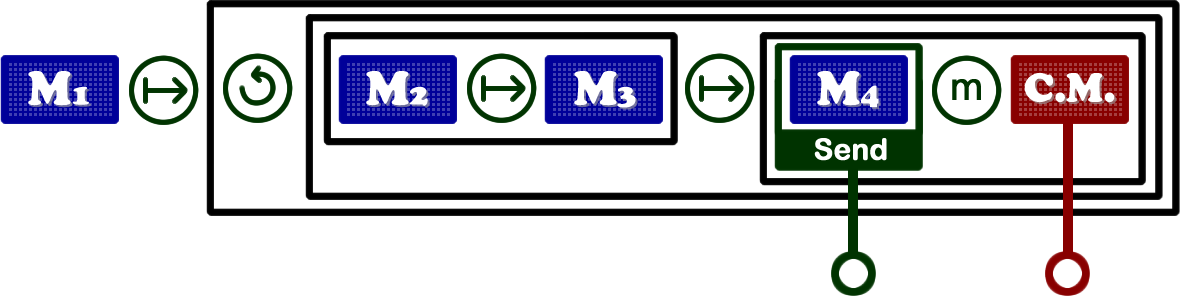
\includegraphics[width=0.6\linewidth]{example_1.png}
	}\\
	\subfloat[][Connecting \posl{} solvers to create \comstrs]{%
		\label{subfig:conn}
		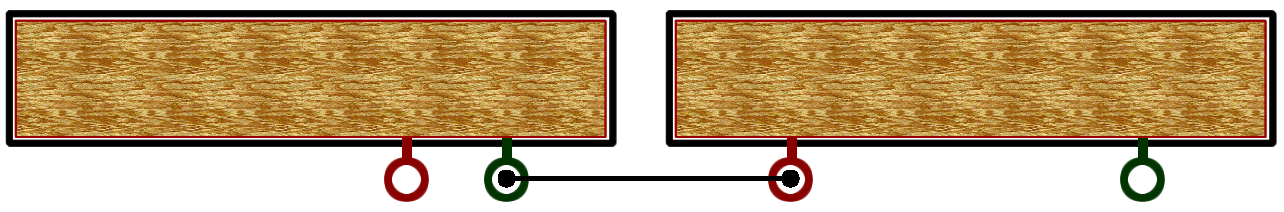
\includegraphics[width=0.6\linewidth]{conn.png}
	}
	\caption[]{Solver construction process using \posl}
	\label{fig:posl}
\end{figure}

%Once the solvers set is ready, the last step is to model the problem to solve. To do so, the user must follow the framework specification to implement the benchmark, respecting some requirements. The most important one is to implement a {\it cost function} computing the cost for a given configuration, i.e., an integer indicating how much the configuration violates the set of constraints. This integer equals zero if the configuration is a solution.

In the following sections all these steps are explained in details, but first, I explain how to model the target benchmark using \posl.

\section{Modeling the target benchmark}
\label{sec:model}

%In this stage we explain formally our modeling process of a benchmark to be solved (or study) through \posl{}. We explain how to make use of the already existing models or to create new benchmarks using the basic layer of the framework in C++ making a proper usage of the object-oriented design.

\modified{Target problems are modelized in \posl{} using the C++ programing language, respecting some rules of the object-oriented design. First of all, the benchmark must inherit from the class \pclass{Benchmark} provided by \posl. This class does not have any method to override or implement, but it receives in its constructor three objects, instances from classes that the user must create, inheriting from \pclass{SolutionCostStrategy}, \pclass{RelativeCostStrategy} and \pclass{ShowStrategy} respectively. In these classes we write the most important functionalities of the benchmark model.}

\underline{\textbf{SolutionCostStrategy}}: \modified{In this class is implemented the strategy to compute the \textit{cost} of a configuration. \posl{} is based on improving step by step an initial configuration, tacking into account a \textit{cost function} provided by the user through the model (implementing the function \pmethod{solutionCost}{$dots$}). The kind of problems that \posl{} solves are the \CSPs{}, so this \textit{cost function} must be a function returning an integer taking into account the problem constraints. Given a configuration $s$, the \textit{cost function}, as a mandatory rule, must return 0 if and only if $s$ is a solution of the problem, i.e., $s$ aims all the problem constraints. An example of \textit{cost function} can be returning the number of violated constraints. However, the more \tet{expressive} is the function cost, the better the behavior of \posl{} is leading to the solution.}

The method to implement in this class is:

\begin{itemize}
\item \verb|int solutionCost(std::vector<int> & c)| $\rightarrow$ It computes the cost of a given configuration (\verb|c|).
\end{itemize}

\underline{\textbf{RelativeCostStrategy}}: \modified{In this classe the user implements the strategy to compute the \textit{cost} of a given configuration, with respect to another: the current one. If the user is able to compute the cost of a configuration, by knowing the performed changes with respect to the current configuration, the search process becomes more efficient, because this function is very often executed.}

The methods to implement in this class are:

\begin{itemize}
\item \verb|void initializeCostData(std::vector<int> & c)| $\rightarrow$ Initializes the information related to the cost (auxiliary data structures, the current configuration (\verb|c|), the current cost, etc.)
\item \verb|void updateConfiguration(std::vector<int> & c)| $\rightarrow$ Updates the information related to the cost.
\item \verb|int relativeSolutionCost(std::vector<int> & c)| $\rightarrow$ Returns the relative cost of the configuration \verb|c| with respect to the current configuration.
\item \verb|int currentCost()| $\rightarrow$ Property that returns the cost of the current configuration.
\item \verb|int costOnVariable(int variable_index)| $\rightarrow$ Returns a measure of how much some variable is contributing to the total cost of a configuration. % \tet{AMPLIAR}
\item \verb|int sickestVariable()| $\rightarrow$ Returns the variable contributing more to the cost.
\end{itemize}

\underline{\textbf{SolutionCostStrategy}}: \modified{This class represents the way a benchmark shows a configuration, in order to be clearer and to give more information about the structure. For example, a configuration of the instance 3--3--2 of the \sgp{} (see bellow for more details about this benchmark) can be written as follows:}

\begin{Verbatim}
[1, 2, 3, 4, 5, 6, 7, 8, 9, 3, 4, 5, 6, 7, 8, 9, 1, 2]
\end{Verbatim}

\modified{But this text is very difficult to read if the instance is bigger. For that reason, the user should implement this class in order to give more details and make easier the configuration read. For example, for the same instance of the problem, a solution is presented as follows:}

\begin{Verbatim}
Golfers: players-3, groups-3, weeks-2
6	8	7	
1	3	5	
4	9	2	
--
7	2	3	
4	8	1	
5	6	9	
--
\end{Verbatim}

The method to implement in this class is:

\begin{itemize}
\item \verb|std::string showSolution(std::shared_ptr<Solution> s)| $\rightarrow$ Returns a string to write in the standard output.
\end{itemize}

\modified{Once we have modelized the target benchmark, we can solve it through \posl{}. In the following sections we describe how to use this parallel-oriented language to solve \CSPs.}

\section{First stage: creating \posl's modules}
\label{sec:1ststage}

There exist two types of basic modules in \posl: \INTROom{} and \INTROopch{}. A \om{} is basically a function and a \opch{} is also a function, but in contrast, it can receive information from two different sources: through input parameters or from outside, i.e., by communicating with a module from another solver.

\subsection{Computation module}

%In this sub-section we expose the definition and the characteristics and the details of the \om, and give some examples. We explain how to create new \oms{} using the basic layer of the framework.

A \om{} is the most basic and abstract way to define a piece of computation. It is a function which receives an instance of a \posl{} data type as input, then executes an internal algorithm, and returns an instance of a \posl{} data type as output. The input and output types will characterize the computation module signature. It can be dy\-na\-mi\-cally replaced by (or combined with) other computation modules, since they can be transmitted to other solvers working in parallel. They are joined through operators defined in Section~\ref{sec:2ndstage}.

\defname{Computation Module}{
A \om{} $Cm$ is a mapping defined by: 
\begin{equation}
\label{def:om}
Cm:I \rightarrow O
\end{equation}
}

where $I$ and $O$, for instance, can be independently a set of configurations, a set of sets of configurations, a set of values of some data type, etc.

Consider a local search meta-heuristic solver. One of its \oms{} can be the function returning the set of configurations composing the neighborhood of a given configuration:

\begin{equation*}
Cm_{neighborhood}:I_1\times I_2\times\dots\times I_n \rightarrow 2^{I_1\times I_2\times\dots\times I_n}
\end{equation*}

\noindent where $I_i$ represents the definition domains of each variable of the input confi\-gura\-tion.

Figure~\ref{fig:om} shows an example of \om: which receives a configuration $S$ and then computes the set $\mathcal{V}$ of its neighbor configurations $\left\{S^1, S^2, \dots, S^m\right\}$.

%\vspace{0.5cm}
\begin{figure}
	\centering	
	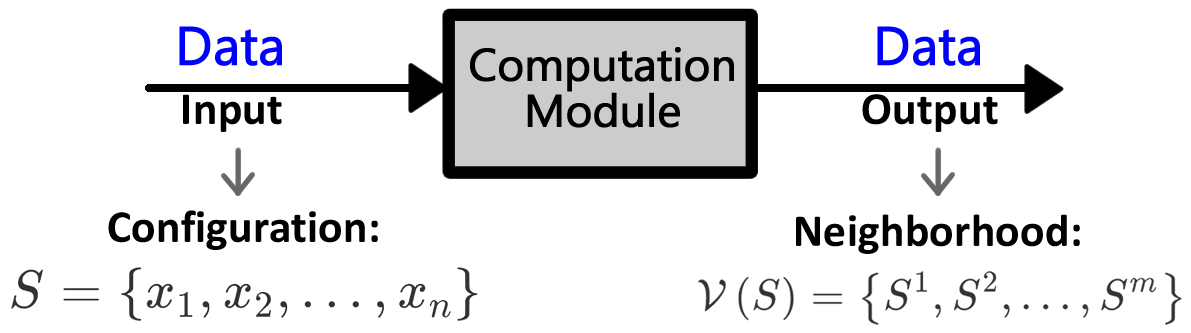
\includegraphics[width=0.7\linewidth]{OM.png}
	\caption{An example of a computation module computing a neighborhood}\label{fig:om}
\end{figure}

\subsubsection{Creating new \oms}
\label{subsubsec:creatingoms}

To create new \oms{} we use C++ programing language. \posl{} provides a hierarchy of data types to work with (see Appendix~\ref{app:diag}) and some abstract classes to inherit from, depending on the type of \om{} the user wants to create. These abstract classes represent {\it abstract} \oms{} and define a type of action to be executed. In the following we present the most important ones:

\begin{itemize}
\item \pclass{ACM\_FirstConfigurationGeneration} $\rightarrow$ Represents \oms{} returning a configuration, usually used for generating the starting configuration on local search meta-heuristics. The user must implement the method \pmethod{execute}{\pclass{ComputationData}} which returns a pointer to a \pclass{Solution}, that is, an object containing all the information concerning a partial solution (configuration, variable domains, etc.)
\item \pclass{ACM\_NeighborhoodFunction} $\rightarrow$ Represent \oms{} receiving a configuration as input and returning its neighborhood as output. The user must implement the method \pmethod{execute}{\pclass{Solution}} which returns a pointer to an object \pclass{Neighborhood}, containing a set of configurations which constitute the neighborhood of a given configuration, according to certain criteria. These configurations are efficiently stored in term of space.
\item \pclass{ACM\_SelectionFunction} $\rightarrow$ Represents \oms{} receiving a neighborhood as input and selecting a configuration from it as output. The user must implement the method \pmethod{execute}{\pclass{Neighborhood}} which returns a pointer to an object \pclass{DecisionPair}, containing two solutions: the current and the selected one.
\item \pclass{ACM\_DecisionFunction} $\rightarrow$ Represents \oms{} receiving a couple af configurations encapsulated into a \pclass{DecisionPair} object, and returning the configuration to be the current one for the next iteration. The user must implement the method \pmethod{execute}{\pclass{DecisionPair}} which returns a pointer to an object \pclass{Solution}.
\item \pclass{ACM\_ProcessingConfigurationFunction} $\rightarrow$ Represents \oms{} receiving a configuration and returning another configuration as result of some arrangement, like for example, a reset. The user must implement the method \pmethod{execute}{\pclass{Solution}} which returns a pointer to an object \pclass{Solution}.
\end{itemize}

\subsection{Communication modules}

%In this sub-section we expose the definition and the characteristics and the details of the \opch, and give some examples. We explain how to create new \opchs{} using the basic layer of the framework.

A \opch{} is the component managing the information reception in the communication between solvers (I talk about information transmission in Section~\ref{sec:2ndstage}). They can interact with \oms{} through operators (see Figure~\ref{fig:och}).

A \opch{} can receive two types of information from an external solver: data or \oms{}. It is important to notice that by sending/receiving \oms, I mean sending/receiving the required information to identify and being able to instantiate the \om. For instance, an integer identifier.

In order to distinguish from the two types of \opchs, I will call \INTROdopch{} the \opch{} responsible for the data reception (Figure~\ref{subfig:doch}), and \INTROoopch{} the one responsible for the reception and instantiation of \oms{} (Figure~\ref{subfig:ooch}).

\defname{Data Communication Module}{
A \emph{Data Communication Module} $Ch$ is a module that produces a mapping defined as follows: 
\begin{equation}
\label{def:dopench}
Ch:I\times \left\{D\cup \left\{NULL\right\}\right\} \rightarrow D \cup \left\{NULL\right\}
\end{equation}
No matter what the input $I$ is, it returns the information $D$ coming from an external solver.
}

\defname{Object Communication Module}{
	If we denote by $\mathbb{M}$ the space of all the \oms{} defined by Definition~\ref{def:om}, then an \emph{\oopch} $Ch$ is a module that produces and executes a \om{} coming from an external solver as follows:
	\begin{equation}
	\label{def:oopench}
	Ch:I\times\left\{\mathbb{M}\cup\left\{NULL\right\}\right\} \rightarrow O \cup \left\{NULL\right\}
	\end{equation}
It returns the output $O$ of the execution of the \om{} coming from an external solver, using $I$ as the input.
}%

\begin{figure}
	\centering
	\subfloat[][Data \opch]{
		\label{subfig:doch}
		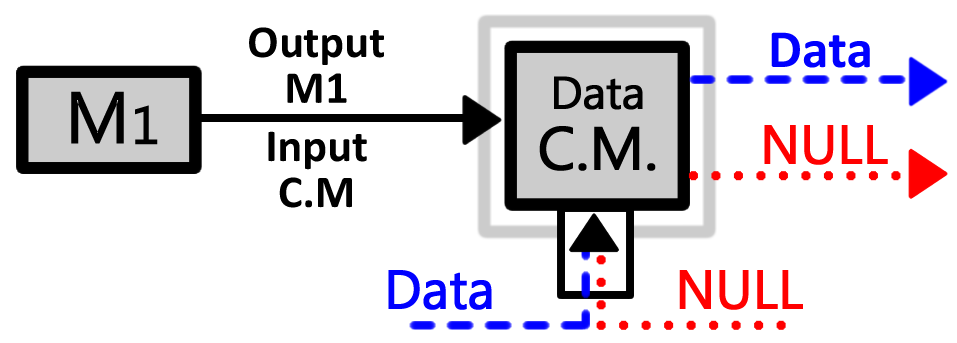
\includegraphics[width=0.4\linewidth]{D_OCh.png}
	}
	\hspace{0.05\textwidth}%
	\subfloat[][Object \opch]{%
		\label{subfig:ooch}
		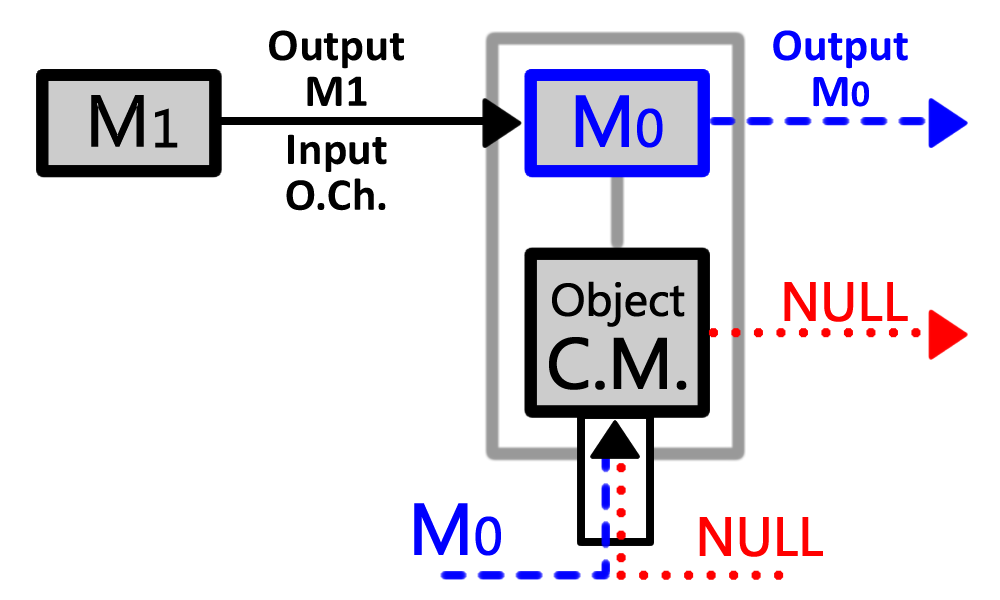
\includegraphics[width=0.4\linewidth]{O_OCh.png}
	}
	\caption[]{Communication module}
	\label{fig:och}
\end{figure}

Users can implement new computation and connection modules but \posl{} already contains many useful modules for solving a broad range of problems.

Due to the fact that \opchs{} receive information coming from outside without having control on them, it is necessary to define the {\it NULL} information, in order to denote the absence of information. If a Data Communication Module receives information, it is returned automatically. If a Object Communication Module receives a \om{}, it is instantiated and executed with the \opch's input and its result is returned. In both cases, if no available information exists (no communications performed), the \opch{} returns the {\it NULL} object.

\section{Second stage: assembling \posl's modules}
\label{sec:2ndstage}

The modules mentioned above are grouped according to their signatures. An \textit{abstract module} is a module that represents all modules with the same signature. For example, the module showed in Figure~\ref{fig:om} is a \om{} based on an abstract module that receives a configuration and returns a neighborhood. %In that sense, an example of a concrete \om{} (or just \om{}) can be a function receiving a configuration, and returning a neighborhood constituted by $N$ configurations which only differ from the input configuration in one entry.

At this stage an \INTROas{} is coded using \posl{}. It takes abstract modules as {\it parameters} and combines them through operators. Through the \as, we can also decide which information to send to other solvers. % by using some operators to send the result of a computation module (see below). In the following we present a formal and more detailed specification of \posl{}'s operators. 

The \as{} is the solver's backbone. It joins the \oms{} and the \opchs{} coherently. It is independent from the \oms{} and \opchs{} used in the solver. It means that modules can be changed or modified during the execution, respecting the algorithm structure. Each time we combine some of them using \posl's operators, we are creating a \INTROcm. Here, we formally define the concept of \textit{module} and \INTROcm.

\begin{definition}
\label{def:module}
A {\bf module} is (Denoted by the letter $\mathcal{M}$):
\begin{enumerate}\renewcommand{\labelitemi}{\scriptsize$\blacksquare$}
\item a \om{}; or
\item a \opch{}; or
\item $\left[\text{OP } \mathcal{M}\right]$, which is the composition of a module $\mathcal{M}$ to be executed sequentially, returning an output depending on the nature of the unary operator \emph{OP}; or\label{subdef:seq_uni}
\item $\left[\mathcal{M}_1 \text{ OP } \mathcal{M}_2\right]$, which is the composition of two modules $\mathcal{M}_1$ and $\mathcal{M}_2$ to be executed sequentially, returning an output depending on the nature of the binary operator \emph{OP}; or\label{subdef:seq}
\item $\parallelexec{\mathcal{M}_1 \text{ OP } \mathcal{M}_2}$, which is the composition of two modules $\mathcal{M}_1$ and $\mathcal{M}_2$ to be executed, returning an output depending on the nature of the binary operator \emph{OP}. These two modules will be executed in parallel if and only if \emph{OP} supports parallelism, %(i.e. some modules will be executed sequentially although they were grouped this way); 
otherwise an exception is thrown.\label{subdef:par}
\end{enumerate}
$\mathbb{M}$ denotes the space of the modules, and we call \cms{} the composition of modules described in \ref{subdef:seq_uni}, \ref{subdef:seq} and/or \ref{subdef:par}.
\end{definition}

For a better understanding of Definition~\ref{def:module}, Figure~\ref{fig:cm} shows graphically  the structure of a \cm.

\begin{figure}[h]
	\centering
	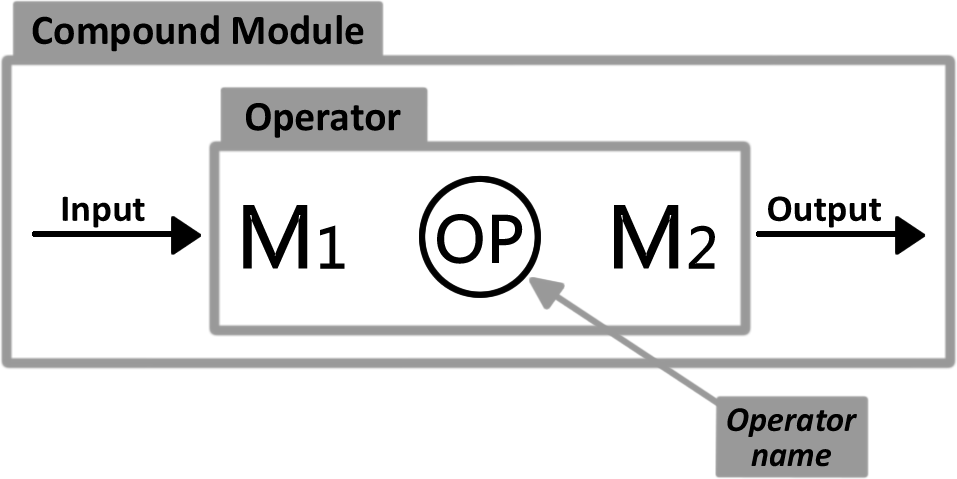
\includegraphics[width=0.5\linewidth]{cm.png}
	\caption[]{A \cm{} made of two modules $M_1$ and $M_2$}
	\label{fig:cm}
\end{figure}

As mentioned before, the \as{} is independent from the \oms{} and \opchs{} used in the solver. It means that one \as{} can be used to construct many different solvers, by implementing it with different modules. %(see below the related concept of \as{} instantiation). 
This is the reason why the \as{} is defined only using {abstract} modules. Formally, we define an \as{} as follows:

\defname{Abstract Solver}{
An \emph{Abstract Solver} $AS$ is a triple $\left(\mathbf{M},\mathcal{L}^m, \mathcal{L}^c\right)$, where: $\mathbf{M}$ is a \cm{} (also called \emph{root \cm{}}), $\mathcal{L}^m$ a list of abstract \oms{} appearing in $\mathcal{M}$, and $\mathcal{L}^c$ a list of \opchs{} appearing in $\mathcal{M}$.}

\Cms{}, and in particular the \textit{root} \cm{}, can be defined also as a context-free grammar as follows.

\begin{definition}\label{def:grammar} A {\bf \cm{}'s grammar} is the set $G_{POSL} = \left(\mathbf{V},\Sigma, \mathbf{S}, \mathbf{R}\right)$, where:
\begin{enumerate}\renewcommand{\labelitemi}{\scriptsize$\blacksquare$}
	\item $\mathbf{V} = \left\{CM, OP\right\}$ is the set of {\it variables},
	\item $\Sigma = \left\{\alpha, \beta, be, [, ], \lbk, \rbk_p, \lsendpar, \rsenddatapar, \rsendmodulepar, \circled{$\mapsto$},\circled{?},\cycop, \circled{$\rho$}, \circled{$\vee$}, \circled{$\wedge$}, \circled{M}, \circled{m}, \circled{$\shortdownarrow$}, \circled{$\cup$}, \circled{$\cap$}\right\}$ is the set of {\it terminals},
	\item $\mathbf{S} = \left\{CM\right\}$ is the set of {\it start variables},
	\item and $\mathbf{R} = $
		\begin{align*} 
		CM \produce & \alpha \OR \beta \OR \senddataop{CM} \OR \sendmoduleop{CM} \OR \left[OP\right] \OR \lbk OP\rbk_p\\
		OP \produce & CM \circled{$\mapsto$} CM \OR CM \circled{?} CM \OR CM \circled{$\rho$} CM \OR CM \circled{$\vee$} CM \OR CM \circled{$\wedge$} CM  \OR\\
		& CM \circled{M} CM \OR CM \circled{m} CM \OR CM \circled{$\shortdownarrow$} CM \OR CM \circled{$\cup$} CM \OR CM \circled{$\cap$} CM  \OR\\
		& \cycop \text{ be } CM%\left\{CM\right\}		
		\end{align*} is a set of {\it rules}
\end{enumerate} 
%For simplicity, we will use, from now on, the name of \emph{Module} to refer ether to an \module, to an \opch, or to a \cm.
\end{definition}

In the following, some of the concepts of Definition~\ref{def:grammar} are explained:
\begin{itemize}
	\item The variables $CM$ and $OP$ correspond to a \cm{} and an {\it operator}, respectively.
	\item The terminals $\alpha$ and $\beta$ represent a \om{} and a \opch{}, respectively.
	\item The terminal $be$ is a Boolean expression.
	\item The terminals $[\text{ } ], \parallelexec{\text{ }}$ are symbols for grouping and defining the way the involved \cms{} are executed. Depending on the nature of the operator, this can be either sequentially or in parallel:
	\begin{enumerate}\renewcommand{\labelitemi}{\scriptsize$\blacksquare$}
		\item $\left[\text{OP}\right]$: The involved operator will always executed sequentially.
		\item $\parallelexec{\text{OP}}$: The involved operator will be executed in parallel if and only if \emph{OP} supports parallelism. Otherwise, an exception is thrown.
	\end{enumerate}
	\item The terminals $\senddataop{.}, \sendmoduleop{.}$ are operators to send information to other solvers (explained bellow).
	\item All other terminals are \posl{} operators that are detailed later.
\end{itemize}

In the following we define \posl{} operators. For grouping modules, like in Definition~\ref{def:module}(\ref{subdef:seq}) and \ref{def:module}(\ref{subdef:par}), we will use $\left|OP\right|$ as a generic grouper. In order to help the reader to easily understand how to use operators, we use an example of a solver that we build step by step, while presenting the definitions.

%\begin{example}
%\mybox{Example}
\poslexample{
\posl{} creates solvers based on local search meta-heuristics algorithms. These algorithms have a common structure: \begin{inparaenum}[1.] \item They start by initializing some data structures (e.g., a \emph{tabu list} for \emph{Tabu Search}, a \emph{temperature} for \emph{Simulated Annealing}, etc.). \item An initial configuration $s$ is generated. \item A new configuration $s'$ is selected from the neighborhood $\mathcal{V}\left(s\right)$. \item If $s'$ is a solution for the problem $P$, then the process stops, and $s'$ is returned. Otherwise, the data structures are updated, and $s'$ is accepted or not for the next iteration, depending on a certain criterion. \end{inparaenum}
%An example of such data structure is the penalizing features of local optima in \emph{Guided Local Search} algorithm.

Abstract \oms{} composing local search meta--heuristics are:

\begin{list}{\boxed{Abstract\hspace{4pt}computation\hspace{4pt}module- \arabic{qcounter}~}}{\usecounter{qcounter}} \itemsep0em 
	\item $I$: Generating a configuration $s$
	\item $V$: Defining the neighborhood $\mathcal{V}\left(s\right)$
	\item $S$: Selecting $s' \in \mathcal{V}\left(s\right)$
	\item $A$: Evaluating an acceptance criterion for $s'$
\end{list}
} %\end{example}

The list of modules to be used in the examples have been presented. Now we present \posl{} operators.

\separation

\begin{definition}\label{op:seqexec}
$\circled{$\mapsto$}$ {\bf Sequential Execution Operator.} Let
\begin{enumerate}%\begin{inparaenum}[i)]
	\item $\mathcal{M}_1 : \mathcal{I}_1 \rightarrow \mathcal{O}_1$ and 
	\item $\mathcal{M}_2 : \mathcal{I}_2 \rightarrow \mathcal{O}_2$, 
\end{enumerate}%\end{inparaenum} 
be modules, where $\mathcal{O}_1 \subseteq \mathcal{O}_2$. Then the operation $\left|\mathcal{M}_1\circled{$\mapsto$} \mathcal{M}_2\right|$ defines the \cm{} $\mathcal{M}_{seq}$ as the result of executing $\mathcal{M}_1$ followed by executing $\mathcal{M}_2$:

\[
\mathcal{M}_{seq}:\mathcal{I}_1 \rightarrow \mathcal{O}_2
\]
\end{definition}

This is an example of an operator that does not support the execution of its involved \cms{} in parallel, because the input of the second \cm{} is the output of the first one.

\poslexample{
Coming back to the example, defined abstract \oms{} can be used to create a \cm{} that performs only one iteration of a local search, using the {\bf Sequential Execution} operator. We create a \cm{} to execute sequentially $I$ and $V$ (see Figure~\ref{subfig:ex_seq1}), then we create another \cm{} to execute sequentially the \cm{} already created and $S$ (see Figure~\ref{subfig:ex_seq2}), and finally this \cm{} and the \om{} $A$ are executed sequentially (see Figure~\ref{subfig:ex_seq3}). The \cm{} presented in Figure~\ref{subfig:ex_seq3} can be coded as follows:
$$\left[\left[\left[I\poslop{\mapsto}V\right]\poslop{\mapsto}S\right]\poslop{\mapsto}A\right]$$
In the figure, each rectangle is a \cm.
}

\begin{figure}[h]
	\centering
	\subfloat[][]{
		\label{subfig:ex_seq1}
		
\includegraphics[width=0.2\linewidth]{seq_1.png}
	}\hspace{0.05\linewidth}
	\subfloat[][]{%
		\label{subfig:ex_seq2}
		
\includegraphics[width=0.3\linewidth]{seq_2.png}
	}\\
	\subfloat[][]{%
		\label{subfig:ex_seq3}
		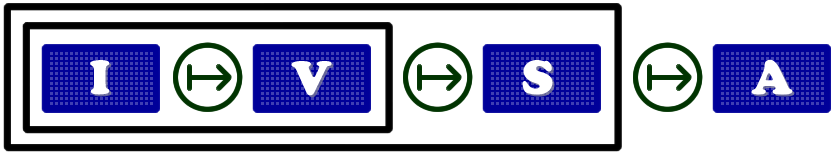
\includegraphics[width=0.4\linewidth]{seq_3.png}
	}
	\caption[]{Using {\bf sequential execution} operator}
	\label{fig:seq_example}
\end{figure}

\separation

The following operator is very useful to execute modules sequentially creating bifurcations, subject to some Boolean condition:

%---------------------------------------------------------
%-----   Conditional Execution Operator
%---------------------------------------------------------
\begin{definition}\label{op:conditional}
$\circled{?}$ {\bf Conditional Execution Operator} Let
\begin{enumerate}%\begin{inparaenum}[i)]
	\item $\mathcal{M}_1 : \mathcal{I} \rightarrow \mathcal{O}_1$ and  
	\item $\mathcal{M}_2 : \mathcal{I} \rightarrow \mathcal{O}_2$,
\end{enumerate}%\end{inparaenum} 
be modules. %, where $\mathcal{D}_1 = \mathcal{D}_2$. %and $\mathcal{I}_1 \subset \mathcal{I}_2$. 
Then the operation $\left|\mathcal{M}_1\circled{?}_{<cond>}\mathcal{M}_2\right|$ defines the \cm{} $\mathcal{M}_{cond}$ as result of the sequential execution of $\mathcal{M}_1$ if $<cond>$ is {\bf true} or $\mathcal{M}_2$, otherwise:

\[
\mathcal{M}_{cond}:\mathcal{I} \rightarrow \mathcal{O}_1 \cup \mathcal{O}_2 
\]
\end{definition}

\poslexample{
This operator can be used in the example if we want to execute two different {\it selection} \oms{} ($S_1$ and $S_2$) depending on certain criterion (see Figure~\ref{fig:cond_example}):
$$\left[\left[\left[I\poslop{\mapsto}V\right]\poslop{\mapsto}\left[S_1\poslop{?}S_2\right]\right]\poslop{\mapsto}A\right]$$
In examples we remove the clause $<cond>$ for simplification.
}

\begin{figure}[h]
	\centering	
	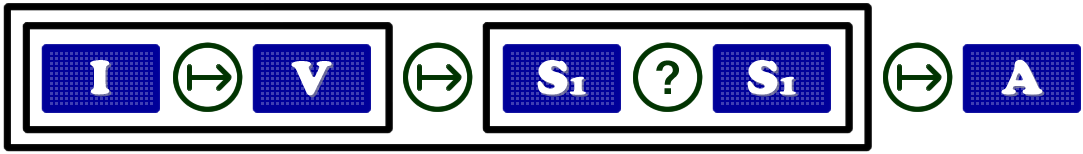
\includegraphics[width=0.5\linewidth]{cond.png}
	\caption{Using {\bf conditional execution} operator}\label{fig:cond_example}
\end{figure}

\separation

We can execute modules sequentially creating also cycles.

%---------------------------------------------------------
%-----   Cyclic Operator
%---------------------------------------------------------

\begin{definition}\label{op:cyclic}
$\cycop$ {\bf Cyclic Execution Operator} Let $\mathcal{M} : \mathcal{I} \rightarrow \mathcal{O}$ be a module, where $\mathcal{O} \subseteq \mathcal{I}$. Then, the operation $\left|\cycop_{<cond>}\mathcal{M}\right|$ defines the \cm{} $\mathcal{M}_{cyc}$ repeating sequentially the execution of $\mathcal{M}$ while $<cond>$ remains {\bf true}:

\[
\mathcal{M}_{cyc}:\mathcal{I} \rightarrow \mathcal{O} 
\]
\end{definition}

\poslexample{
Using this operator we can model a local search algorithm, by executing the {\it abstract} \om{} $I$ and then the other \oms{} ($V$, $S$ and $A$) cyclically, until finding a solution (\ie a configuration with cost equals to zero) (see Figure~\ref{fig:cyc_example}):
$$\left[I\poslop{\mapsto}\left[\cycop\left[\left[V\poslop{\mapsto}S\right]\poslop{\mapsto}A\right]\right]\right]$$
In the examples, we remove the clause $<cond>$ for simplification. 
}

\begin{figure}[h]
	\centering	
	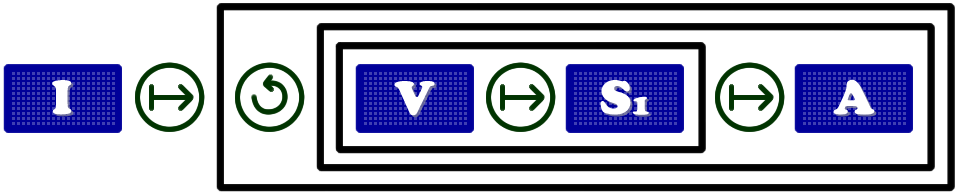
\includegraphics[width=0.5\linewidth]{cyc.png}
	\caption{Using {\bf cyclic execution} operator}\label{fig:cyc_example}
\end{figure}

\separation

%---------------------------------------------------------
%-----   Random Choice Operator
%---------------------------------------------------------
\begin{definition}\label{op:rho}
$\circled{$\rho$}$ {\bf Random Choice Operator} Let
\begin{enumerate}%\begin{inparaenum}[i)]
	\item $\mathcal{M}_1 : \mathcal{I} \rightarrow \mathcal{O}_1$ and  
	\item $\mathcal{M}_2 : \mathcal{I} \rightarrow \mathcal{O}_2$,
\end{enumerate}%\end{inparaenum} 
be modules. %, where $\mathcal{D}_1 = \mathcal{D}_2$, % and $\mathcal{I}_1 \subset \mathcal{I}_2$, 
and a real value $\rho \in (0,1)$. Then the operation $\left|M_1\circled{$\rho$}\mathcal{M}_2\right|$ defines the \cm{} $\mathcal{M}_{rho}$ executing $\mathcal{M}_1$ with probability $\rho$, or executing $\mathcal{M}_2$ with probability $(1-\rho)$:

\[
\mathcal{M}_{rho}:\mathcal{I} \rightarrow \mathcal{O}_1 \cup \mathcal{O}_2 
\]
\end{definition}

\poslexample{
In the example we can create a \cm{} to execute two {\it abstract} \oms{} $A_1$ and $A_2$ following certain probability $\rho$ using the {\bf random choice} operator as follows (see Figure~\ref{fig:rho_example}):
$$\left[I\poslop{\mapsto}\left[\cycop\left[\left[V\poslop{\mapsto}S\right]\poslop{\mapsto}\left[A_1\poslop{\rho}A_2\right]\right]\right]\right]$$
}

\begin{figure}[h]
	\centering	
	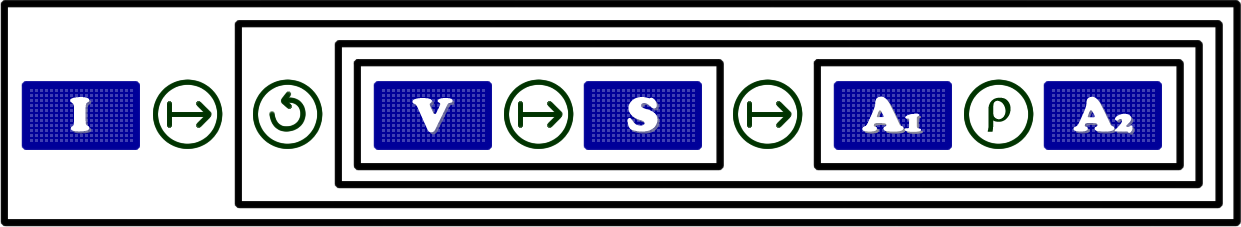
\includegraphics[width=0.6\linewidth]{rho.png}
	\caption{Using {\bf random choice} operator}\label{fig:rho_example}
\end{figure}

\separation

The following operator is very useful if the user needs to use a \opch{} inside an \as{}. As explained before, if a \opch{} does not receive any information from another solver, it returns {\it NULL}. This may cause the undesired termination of the solver if this case is not correctly handled. Next, we introduce the \textbf{Not {\it NULL} Execution Operator} and illustrate how to use it in practice with an example.

%---------------------------------------------------------
%-----   Not Null Operator
%---------------------------------------------------------
\begin{definition}\label{op:or}
$\circled{$\vee$}$ {\bf Not {\it NULL} Execution Operator} Let
\begin{enumerate}%\begin{inparaenum}[i)]
	\item $\mathcal{M}_1 : \mathcal{I} \rightarrow \mathcal{O}_1$ and  
	\item $\mathcal{M}_2 : \mathcal{I} \rightarrow \mathcal{O}_2$,
\end{enumerate}%\end{inparaenum} 
be modules. %, where $\mathcal{D}_1 = \mathcal{D}_2$. % and $\mathcal{I}_1 \subset \mathcal{I}_2$. 
Then, the operation $\left|\mathcal{M}_1\circled{$\vee$}\mathcal{M}_2\right|$ defines the \cm{} $\mathcal{M}_{non}$ that executes $\mathcal{M}_1$ and returns its output if it is not {\it NULL}, or executes $\mathcal{M}_2$ and returns its output otherwise:

\[
\mathcal{M}_{non}:\mathcal{I} \rightarrow \mathcal{O}_1 \cup \mathcal{O}_2 
\]
\end{definition}

\poslexample{Let us consider a slightly more complex example: when applying the acceptance criterion, suppose that we want to receive a configuration from other solver to combine the \om{} $A$ with a \opch:

\begin{list}{\boxed{Communication\hspace{4pt}module- \arabic{qcounter}:~}}{\usecounter{qcounter}} \itemsep0em
	\item $C.M.$: Receiving a configuration.\label{struct:opch}
\end{list}

Figure~\ref{fig:2difBeh} shows how to combine a \opch{} with the \om{} $A$ through the operator $\circled{$\vee$}$. Here, the \om{} $A$ will be executed as long as the \opch{} remains \textit{NULL}, i.e., there is no information coming from outside. This behavior is represented in Figure~\ref{subfig:beh1} by the blue lines. If some data has been received through the \opch, the later is executed instead of the module $A$, represented in Figure~\ref{subfig:beh2} by orange lines. 
The code can be written as follows:
$$\left[I\poslop{\mapsto}\left[\cycop\left[\left[V\poslop{\mapsto}S\right]\poslop{\mapsto}\left[C.M.\poslop{\vee}A\right]\right]\right]\right]$$
}

\begin{figure}[h]
\centering
\subfloat[][The solver executes the computation module {\bf A} if no information is received through the connection module]{
	\label{subfig:beh1}
	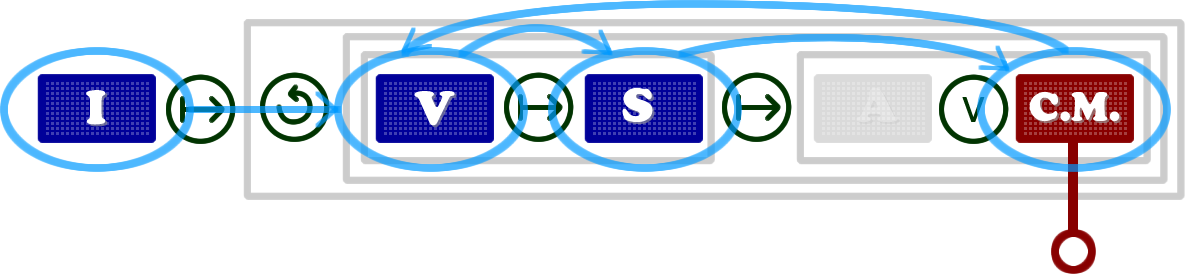
\includegraphics[width=0.6\linewidth]{muta2_v4.png}
}\\
%\hspace{0.05\textwidth}%
\subfloat[][The solver uses the information coming from an external solver]{%
	\label{subfig:beh2}
	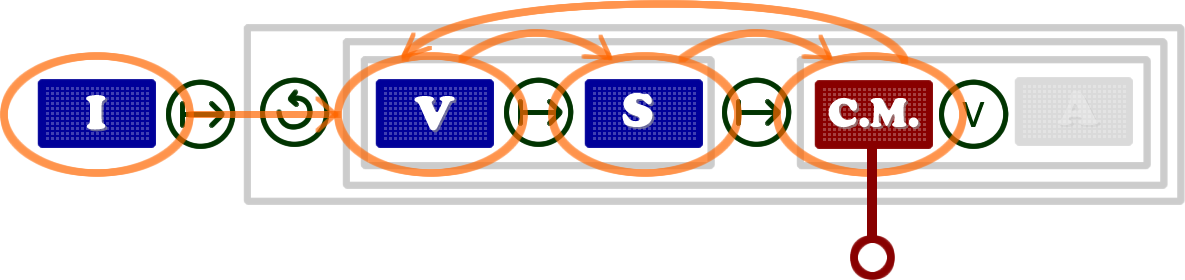
\includegraphics[width=0.6\linewidth]{muta1_v4.png}
}
\caption[]{Two different behaviors within the same solver}
\label{fig:2difBeh}
\end{figure}

\separation

The operator that we have just defined is a {\it short-circuit} operator. It means that if the first argument (module) does not return {\it NULL}, the second will not be executed. \posl{} provides another operator with the same functionality but not {\it short-circuit}. This operator is necessary if the user wants a side effect by always executing the second module also.

%---------------------------------------------------------
%-----   BOTH Operator
%---------------------------------------------------------

\begin{definition}\label{op:and}
$\circled{$\wedge$}$ {\bf {\it BOTH} Execution Operator} Let 
\begin{enumerate}%\begin{inparaenum}[i)]
	\item $\mathcal{M}_1 : \mathcal{I} \rightarrow \mathcal{O}_1$ and  
	\item $\mathcal{M}_2 : \mathcal{I} \rightarrow \mathcal{O}_2$,
\end{enumerate}%\end{inparaenum} 
be modules. %, where $\mathcal{D}_1 \subseteq \mathcal{D}_2$. % and $\mathcal{I}_1 \subset \mathcal{I}_2$. 
Then the operation $\left|\mathcal{M}_1\circled{$\wedge$}\mathcal{M}_2\right|$ defines the \cm{} $\mathcal{M}_{both}$ that executes both $\mathcal{M}_1$ and $\mathcal{M}_2$, then returns the output of $\mathcal{M}_1$ if it is not {\it NULL}, or the output of $\mathcal{M}_2$ otherwise:

\[
\mathcal{M}_{both}:\mathcal{I} \rightarrow \mathcal{O}_1 \cup \mathcal{O}_2 
\]
\end{definition}

\separation

In the following we introduce the concepts of {\it cooperative parallelism} and {\it competitive parallelism}. We say that cooperative parallelism exists when two or more processes are running separately, and the general result will be some combination of the results of at least some involved processes (e.g. Definitions~\ref{op:min} and~\ref{op:max}). On the other hand, competitive parallelism arise when the general result comes from an unique process, usialy the one finishing first (e.g. Definition~\ref{op:race}).

%---------------------------------------------------------
%-----   MIN Operator
%---------------------------------------------------------

\begin{definition}\label{op:min}
$\circled{m}$ {\bf Minimum Operator } Let
\begin{enumerate}%\begin{inparaenum}[i)]
	\item $\mathcal{M}_1 : \mathcal{I} \rightarrow \mathcal{O}_1$ and  
	\item $\mathcal{M}_2 : \mathcal{I} \rightarrow \mathcal{O}_2$,
\end{enumerate}%\end{inparaenum} 
be modules. %, where $\mathcal{D}_1 \subseteq \mathcal{D}_2$. %and $\mathcal{I}_1 \subset \mathcal{I}_2$. 
Let also $o_1$ and $o_2$ be the outputs of $\mathcal{M}_1$ and $\mathcal{M}_2$, respectively. Assume that there exists a total order in $O_1 \cup O_2$ where the object \emph{NULL} is the greatest value. Then the operation $\left|\mathcal{M}_1\circled{m}\mathcal{M}_2\right|$ defines the \cm{} $\mathcal{M}_{min}$ that executes $\mathcal{M}_1$ and $\mathcal{M}_2$, and returns $\min\left\{o_1,o_2\right\}$:

\[
\mathcal{M}_{min}:\mathcal{I} \rightarrow \mathcal{O}_1 \cup \mathcal{O}_2 
\]
\end{definition}

\separation

Similarly we define the \textbf{Maximum} operator:

%---------------------------------------------------------
%-----   MAX Operator
%---------------------------------------------------------

\begin{definition}\label{op:max}
$\circled{M}$ {\bf Maximum Operator} Let
\begin{enumerate}%\begin{inparaenum}[i)]
	\item $\mathcal{M}_1 : \mathcal{I} \rightarrow \mathcal{O}_1$ and  
	\item $\mathcal{M}_2 : \mathcal{I} \rightarrow \mathcal{O}_2$,
\end{enumerate}%\end{inparaenum} 
be modules. %, where $\mathcal{D}_1 \subseteq \mathcal{D}_2$. %and $\mathcal{I}_1 \subset \mathcal{I}_2$. 
Let also $o_1$ and $o_2$ be the outputs of $\mathcal{M}_1$ and $\mathcal{M}_2$, respectively. Assume that there exists a total order in $O_1 \cup O_2$ where the object \emph{NULL} is the smallest value. Then the operation $\left|\mathcal{M}_1\circled{M}\mathcal{M}_2\right|$ defines the \cm{} $\mathcal{M}_{max}$ that executes $\mathcal{M}_1$ and $\mathcal{M}_2$, and returns $\max\left\{o_1,o_2\right\}$:

\[
\mathcal{M}_{max}:\mathcal{I} \rightarrow \mathcal{O}_1 \cup \mathcal{O}_2 
\]
\end{definition}

\poslexample{The {\bf minimum operator} can be applied in the previews example to obtain an interesting behavior: When applying the acceptance criteria, suppose that we want to receive a configuration from another solver, to compare it with ours and select the one with the lowest cost. We can do that by applying the $\circled{m}$ operator to combine the \om{} $A$ with a \opch{} $C.M.$ (see Figure\ref{fig:min_example}):
$$\left[I\poslop{\mapsto}\left[\cycop\left[\left[V\poslop{\mapsto}S\right]\poslop{\mapsto}\lbk A\poslop{m}C.M.\rbk_p\right]\right]\right]$$
Notice that in this example, we can use the grouper $\lbk .\rbk_p$ since the {\bf minimum operator} supports parallelism.}

\begin{figure}[h]
	\centering	
	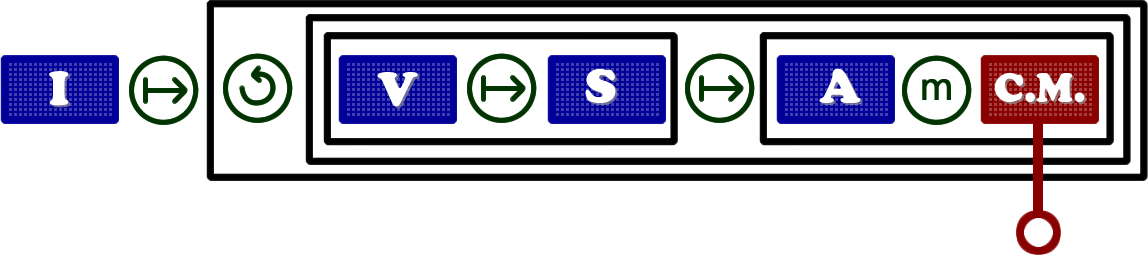
\includegraphics[width=0.6\linewidth]{min.png}
	\caption{Using {\bf minimum} operator}\label{fig:min_example}
\end{figure}

\separation

%---------------------------------------------------------
%-----   Race Operator
%---------------------------------------------------------

\begin{definition}\label{op:race}
$\circled{$\shortdownarrow$}$ {\bf Race Operator} Let 
\begin{enumerate}%\begin{inparaenum}[i)]
	\item $\mathcal{M}_1 : \mathcal{I} \rightarrow \mathcal{O}_1$ and  
	\item $\mathcal{M}_2 : \mathcal{I} \rightarrow \mathcal{O}_2$,
\end{enumerate}%\end{inparaenum} 
be modules. %, where $\mathcal{I}_1 \subseteq \mathcal{I}_2$ and $\mathcal{O}_1 \subset \mathcal{O}_2$. 
Then the operation $\left|\mathcal{M}_1\circled{$\shortdownarrow$}\mathcal{M}_2\right|$ defines the \cm{} $\mathcal{M}_{race}$ that executes both modules $\mathcal{M}_1$ and $\mathcal{M}_2$, and returns the output of the module ending first:

\[
\mathcal{M}_{race}:\mathcal{I} \rightarrow \mathcal{O}_1 \cup \mathcal{O}_2 
\]
\end{definition}

\poslexample{Sometimes nighborhood functions are slow depending on the configuration. In that case two neighborhood \oms{} can be executed and we take into account the output of the module ending first (see Figure\ref{fig:race_example}):
$$\left[I\poslop{\mapsto}\left[\cycop\left[\left[\lbk V_1\poslop{\shortdownarrow}V_2\rbk_p\poslop{\mapsto}S\right]\poslop{\mapsto}\lbk A\poslop{m}C.M.\rbk_p\right]\right]\right]$$}

\begin{figure}[h]
	\centering	
	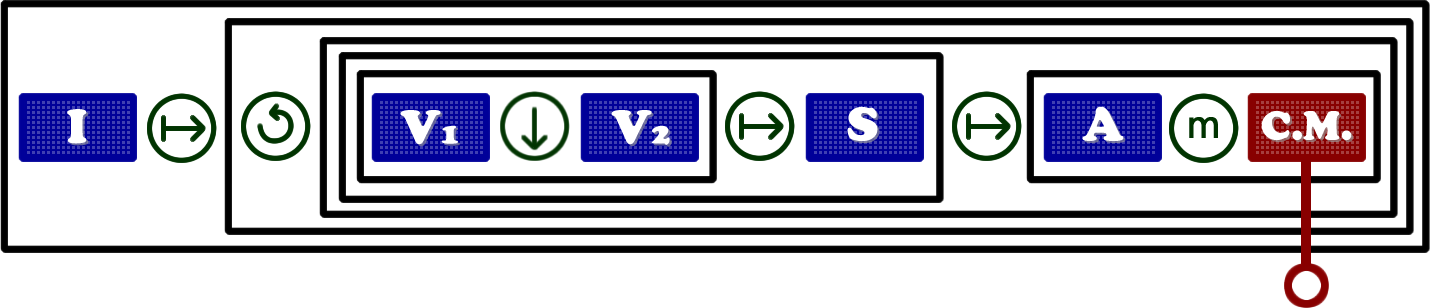
\includegraphics[width=0.7\linewidth]{race.png}
	\caption{Using {\bf race} operator}\label{fig:race_example}
\end{figure}

\separation

Some \posl's data types are related to sets, like neighborhoods. For that reason, it is useful to define operators to handle that kind of data. Although at this moment \posl{} is designed only to create solvers based on local-search meta-heuristic, is was conceived to be able to create population-based solvers as a future direction. In that sens, these operators are also useful.

\begin{definition}\label{op:union}
$\circled{$\cup$}$ {\bf Union Operator} Let 
\begin{enumerate}%\begin{inparaenum}[i)]
	\item $\mathcal{M}_1 : \mathcal{I} \rightarrow \mathcal{O}_1$ and  
	\item $\mathcal{M}_2 : \mathcal{I} \rightarrow \mathcal{O}_2$,
\end{enumerate}%\end{inparaenum} 
be modules. %, where $\mathcal{D}_1 \subseteq \mathcal{D}_2$. %and $\mathcal{I}_1 \subset \mathcal{I}_2$. 
Let also the sets $V_1$ and $V_2$ be the outputs of $\mathcal{M}_1$ and $\mathcal{M}_2$, respectively. Then the operation $\left|\mathcal{M}_1\circled{$\cup$}\mathcal{M}_2\right|$ defines the \cm{} $\mathcal{M}_{\cup}$ that executes both modules $\mathcal{M}_1$ and $\mathcal{M}_2$, and returns $V_1\cup V_2$:

\[
\mathcal{M}_{\cup}:\mathcal{I} \rightarrow \mathcal{O}_1 \cup \mathcal{O}_2
\]
\end{definition}

\separation

Similarly we define the operators \textbf{Intersection} and \textbf{Subtraction}:

\begin{definition}\label{op:intersec}
$\circled{$\cap$}$ {\bf Intersection Operator} Let 
\begin{enumerate}%\begin{inparaenum}[i)]
	\item $\mathcal{M}_1 : \mathcal{I} \rightarrow \mathcal{O}_1$ and  
	\item $\mathcal{M}_2 : \mathcal{I} \rightarrow \mathcal{O}_2$,
\end{enumerate}%\end{inparaenum} 
be modules. %, where $\mathcal{D}_1 \subseteq \mathcal{D}_2$. % and $\mathcal{I}_1 \subset \mathcal{I}_2$. 
Let also the sets $V_1$ and $V_2$ be the outputs of $\mathcal{M}_1$ and $\mathcal{M}_2$, respectively. Then the operation $\left|\mathcal{M}_1\circled{$\cap$}\mathcal{M}_2\right|$ defines the \cm{} $\mathcal{M}_{\cap}$ that executes both modules $\mathcal{M}_1$ and $\mathcal{M}_2$, and returns $V_1\cap V_2$:

\[
\mathcal{M}_{\cap}:\mathcal{I} \rightarrow \mathcal{O}_1 \cup \mathcal{O}_2
\]
\end{definition}

\separation

\begin{definition}\label{op:subst}
$\circled{$\setminus$}$ {\bf Subtraction Operator} Let 
\begin{enumerate}%\begin{inparaenum}[i)]
	\item $\mathcal{M}_1 : \mathcal{I} \rightarrow \mathcal{O}_1$ and  
	\item $\mathcal{M}_2 : \mathcal{I} \rightarrow \mathcal{O}_2$,
\end{enumerate}%\end{inparaenum} 
be modules. %, where $\mathcal{D}_1 \subseteq \mathcal{D}_2$. % and $\mathcal{I}_1 \subset \mathcal{I}_2$. 
Let also $V_1$ and $V_2$ be the outputs of $\mathcal{M}_1$ and $\mathcal{M}_2$, respectively. Then the operation $\left|\mathcal{M}_1\circled{$\setminus$}\mathcal{M}_2\right|$ defines the \cm{} $\mathcal{M}_{\setminus}$ that executes both modules $\mathcal{M}_1$ and $\mathcal{M}_2$, and returns $V_1 \setminus V_2$:

\[
\mathcal{M}_{\setminus}:\mathcal{I} \rightarrow \mathcal{O}_1
\]
\end{definition}

\separation

Now, we define the operators which allow to send information to other solvers. Two types of information can be sent: 
\begin{inparaenum}[i)]
	\item the output of the \om{} as result of its execution, or 
	\item the \om{} itself.
\end{inparaenum} This feature is very useful in terms of sharing behaviors between solvers.

\begin{definition}\label{op:osend}
$\senddataop{.}$ {\bf Sending Data Operator} Let $\mathcal{M} : \mathcal{I} \rightarrow \mathcal{O}$ be a module. Then the operation $\left|\senddataop{\mathcal{M}}\right|$ defines the \cm{} $\mathcal{M}_{sendD}$ that executes the module $\mathcal{M}$ and sends its output to a \opch:

\[
\mathcal{M}_{sendD}:\mathcal{I} \rightarrow \mathcal{O}
\]
\end{definition}

\separation

Similarly we define the \textbf{Send Module} operator:

\begin{definition}\label{op:msend}
$\sendmoduleop{.}$ {\bf Sending Module Operator} Let $\mathcal{M} : \mathcal{I} \rightarrow \mathcal{O}$ be a module. Then the operation $\left|\sendmoduleop{\mathcal{M}}\right|$ defines the \cm{} $\mathcal{M}_{sendM}$ that executes the module $\mathcal{M}$, then returns its output and sends the module itself to a \opch:

\[
\mathcal{M}_{sendM}:\mathcal{I} \rightarrow \mathcal{O}
\]
\end{definition}

\poslexample{In the following example, we use one of the \cms{} already presented in the previews examples, using a \opch{} to receive a configuration (see Figure~\ref{subfig:receiver_example}):  
$$\left[I\poslop{\mapsto}\left[\cycop\left[\left[V\poslop{\mapsto}S\right]\poslop{\mapsto}\lbk A\poslop{m}C.M.\rbk_p\right]\right]\right]$$

We also build another, as its complement: sending the accepted configuration to outside, using the {\bf sending data operator} (see Figure\ref{subfig:sender_example}):
$$\left[I\poslop{\mapsto}\left[\cycop\left[\left[V\poslop{\mapsto}S\right]\poslop{\mapsto}\senddataop{A}\right]\right]\right]$$

In the Section~\ref{sec:4thstage} we explain how to connect solvers to each other.
}

\begin{figure}[h]
\centering
\subfloat[][]{
	\label{subfig:receiver_example}
	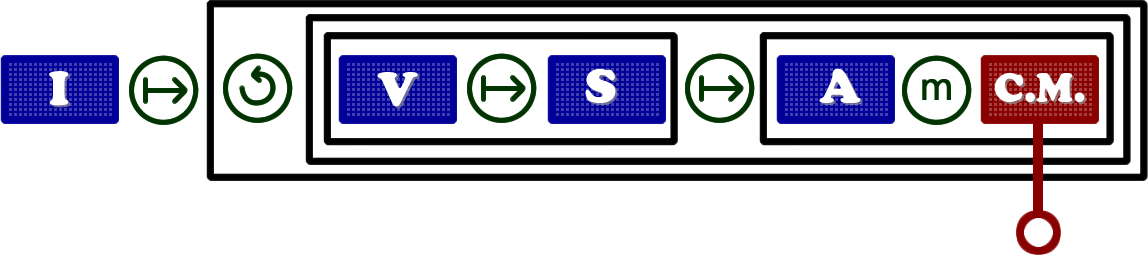
\includegraphics[width=0.6\linewidth]{min.png}
}\\
\subfloat[][]{%
	\label{subfig:sender_example}
	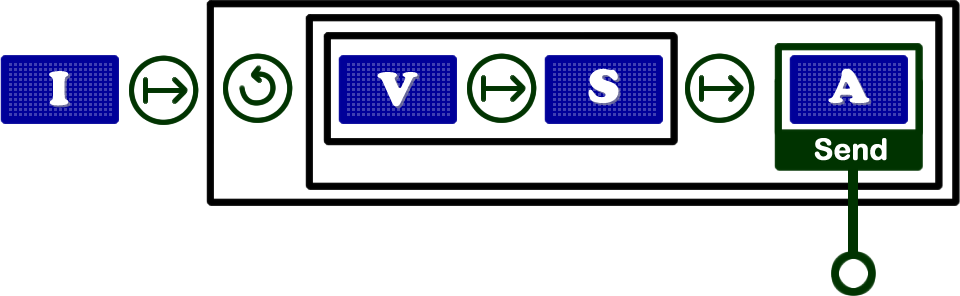
\includegraphics[width=0.6\linewidth]{send.png}
}
\caption[]{Sender and receiver behaviors}
\label{fig:send_recv}
\end{figure}

Sending \ms{} through this operator is performed by sending an identifier, in the case of \oms, or the corresponding \posl{} code in the case of \cms. The receptor \dopch{} creates the \m, executes it and returns its output. There exists other ways to do this task more efficiently, for example, compiling modules in a pre--processing stage and store them in memory, to be executed afterwards by sending only the reference. However, \posl{} does it this way, because it was thought to be able to apply learning techniques to the received modules in the future, and to adapt them to the experience of the solver during the search.

\separation

Once all desired abstract modules are linked together with operators, we obtain the root \cm{}, i.e., the algorithmic part of an \as. To implement a concrete solver from an \as, one must instantiate each abstract module with a concrete one respecting the required signature. From the same \as, one can implement many different concrete solvers simply by instantiating abstract modules with different concrete modules.

An \as{} is declared as follows: after declaring the \mbox{\tet{\bf \as}}'s name, the first line defines the list of abstract \oms, the second one the list of abstract \opchs, then the algorithm of the solver is defined as the solver's body (the root \cm{} $\mathbf{M}$), between \mbox{\tet{\bf begin}} and \mbox{\tet{\bf end}}.

An \as{} can be declared through the  simple regular expression:

\begin{center}
\tet{\bf abstract solver} {\it name} \tet{\bf computation}: $\mathcal{L}^m$ (\tet{\bf communication}: $\mathcal{L}^c$)? \tet{\bf begin} $\mathbf{M}$ \tet{\bf end}
\end{center}

where:
\begin{itemize}
\item {\it name} is the identifier of the \as{}, 
\item $\mathcal{L}^m$ is the list of abstract \oms{},
\item $\mathcal{L}^c$ is the list of abstract \opchs{}, and
\item $\mathbf{M}$ is the root \cm.
\end{itemize}

For instance, Algorithm~\ref{algo:as_example} illustrates the abstract solver corresponding to Figure~\ref{subfig:sender_example}.% Figure~\ref{subfig:as}.

\begin{algorithm}[H]
\dontprintsemicolon
\SetNoline
\SetKwProg{myproc}{}{}{}
\myproc{\tet{\bf abstract solver} as\_01\;
\tet{\bf computation} : $I, V, S, A$ \; 
\tet{\bf connection}: $C.M.$}{
	\Begin{
		$I\poslop{\mapsto}$
		\whileinline{$\left(\textbf{\Iter < } K_1\right)$}{
			$\left[V\poslop{\mapsto}S\poslop{\mapsto}\senddataop{A}\right]$ %\left[C.M.\poslop{m} \senddataop{A}\right]\right]$
		}
	}
}
\caption{\posl{} pseudo-code for the \as{} presented in Figure~\ref{subfig:sender_example}}\label{algo:as_example}
%\caption{\posl{} pseudo-code for the \as{} presented in Figure~\ref{subfig:as}}\label{algo:as_example}
\end{algorithm}	

\section{Third stage: creating \posl{} solvers}
\label{sec:3rdstage}

%With operation modules and open channels already assembled through the \as, we can create solvers by instantiating modules. \posl{} provides an environment to this end and we present the procedure to use it.

%With \module s, \opch s and \cstr{} defined, we can create solvers by instantiating the declared components. \af{} provides an environment to this end, presented in Algorithm~\ref{algo:solver_def}, where $m_i$ and $ch_i$ represent the instances of the \module s and the instances of the \opch s to be passed by parameters to the \cstr{} $St$.

With \bothmodules{} composing an \as, one can create solvers by instantiating \ms. This is simply done by specifying that a given \mbox{\tet{\bf solver}} must \mbox{\tet{\bf implements}} a given \as, followed by the list of \omprefix{} then \opchs{}. These modules must match signatures required by the \as. Algorithm~\ref{algo:solver_def} implements Algorithm~\ref{algo:as_example} by instantiating modules shown in Figure~\ref{fig:2difBeh}.

\begin{algorithm}[H]
\dontprintsemicolon
\SetNoline
\SetKwProg{myproc}{}{}{}
%\myproc{
\tet{\bf solver} solver\_01 \tet{\bf implements} as\_01\;
\tet{\bf computation} : $I_{rand}, V_{std}, S_{best}, A_{alw}$ \; 
\tet{\bf connection}: $CM_{last}$\; %}{
%	\Begin{
%	}
%}
\caption{An instantiation of the \as{} presented in Algorithm~\ref{algo:as_example}}\label{algo:solver_def}
\end{algorithm}

Algorithm~\ref{algo:solver_def} is just an example of a solver instantiation, using some \oms{} provided by \posl{}, that are used and explained in details in the Chapter~\ref{chap:expe} of this document:
\begin{itemize}
\item $I_{rand}$ creates a random configuration.
\item $V_{std}$ creates a neighborhood of a given configuration, changing one element at a time.
\item $S_{best}$ selects the configuration of a neighborhood with the lowest cost.
\item $A_{alw}$ always accepts the incoming configuration.
\item $CM_{last}$ returns the last configuration arrived, if at the time of its execution, there is more than one configuration waiting to be received. 
\end{itemize}

\section{Forth stage: connecting the solvers}
\label{sec:4thstage}

Once a set of solvers is created, the last stage is to connect them to each other. Up to this point, solvers are disconnected, but they are ready to establish the communication. \posl{} provides tools  to the user to easily define cooperative strategies based on communication jacks and outlets. The pool of (concrete) connected solvers to be executed in parallel to solve a problem is called a \INTROsoset{}. 

%In the following we present two important concepts necessary to formalize \INTROcommoper.

\begin{definition}\label{def:comm_jack}
{\bf Communication Jack} Let $\mathcal{S}$ be a solver and a module $\mathcal{M}$. Then the operation $\mathcal{S}\cdot\mathcal{M}$ opens an outgoing connection from the solver $\mathcal{S}$, sending either 
\begin{inparaenum}[a)]
	\item the output of $\mathcal{M}$, if a sending data operator is applied to $\mathcal{M}$, as presented in Definition~\ref{op:osend}, or
	\item $\mathcal{M}$ itself, if a sending module operator is applied to $\mathcal{M}$, as presented in Definition~\ref{op:msend}.
\end{inparaenum}
\end{definition} 

\begin{definition}\label{def:comm_outlet}
{\bf Communication Outlet} Let $\mathcal{S}$ be a solver and a \opch{} $\mathcal{CM}$. Then, the operation $\mathcal{S}\cdot\mathcal{CM}$ opens an ingoing connection to the solver $\mathcal{S}$, receiving either 
\begin{inparaenum}[a)]
	\item the output of some \om{}, if $\mathcal{CM}$ is a \dopch{}, or
	\item a \om{}, if $\mathcal{CM}$ is an \oopch.
\end{inparaenum}
\end{definition} 

\separation

The communication is established by following the following rules guideline:
\begin{enumerate}%\begin{inparaenum}
	\item Each time a solver sends any kind of information by using a {\it sending} operator, it creates a \INTROjack.
	\item Each time a solver defines a \opch, it creates a \INTROoutlet. 
	\item Solvers can be connected to each other by linking \jacks{} to \outlets.
\end{enumerate} %\end{inparaenum}

%With the operator $(\cdot)$ we can have access to \oms{} sending information and to the \opch's names in a solver. 
%For example: $Solver_0\cdot \mathcal{M}$ provides access to the \om{} $\mathcal{M}$ in $Solver_0$ if and only if it is affected by a {\it sending} operator, and $Solver_1\cdot CM$ provides access to the \opch{} $CM$ in $Solver_1$.

Following, we define \textit{connection operators} that \posl{} provides.

\begin{definition}\label{op_conn:1to1}
\onetoone {\bf Connection One-to-One Operator} Let 
\begin{enumerate}
\item $\mathcal{J} = \left[\mathcal{S}_0\cdot \mathcal{M}_0, \mathcal{S}_1\cdot \mathcal{M}_1,\dots, \mathcal{S}_{N-1}\cdot \mathcal{M}_{N-1}\right]$ be the list of \jacks, and
\item $\mathcal{O} = \left[\mathcal{Z}_0\cdot \mathcal{CM}_0, \mathcal{Z}_1\cdot \mathcal{CM}_1,\dots, \mathcal{Z}_{N-1}\cdot \mathcal{CM}_{N-1}\right]$ be the list of \outlets{}
\end{enumerate} Then the operation 
\[
\mathcal{J} \onetoonesep \mathcal{O}
\]
connects each \jack{} $\mathcal{S}_i\cdot \mathcal{M}_i \in \mathcal{J}$ with the corresponding \outlet{} $\mathcal{Z}_i\cdot \mathcal{CM}_i \in \mathcal{O}$, $\forall\textbf{ }0 \leq i \leq N-1$ (see Figure~\ref{subfig:comm_simple}).
\end{definition}

\separation

\begin{definition}\label{op_conn:1ton}
\oneton {\bf Connection One-to-N Operator} Let 
\begin{enumerate} 
\item $\mathcal{J} = \left[\mathcal{S}_0\cdot \mathcal{M}_0, \mathcal{S}_1\cdot \mathcal{M}_1,\dots, \mathcal{S}_{N-1}\cdot \mathcal{M}_{N-1}\right]$ be the list of \jacks, and 
\item $\mathcal{O} = \left[\mathcal{Z}_0\cdot \mathcal{CM}_0, \mathcal{Z}_1\cdot \mathcal{CM}_1,\dots, \mathcal{Z}_{M-1}\cdot \mathcal{CM}_{M-1}\right]$ be the list of \outlets{} 
\end{enumerate} Then the operation 
\[
\mathcal{J} \onetonsep \mathcal{O}
\]
connects each \jack{} $\mathcal{S}_i\cdot \mathcal{M}_i \in \mathcal{J}$ with every \outlet{} $\mathcal{Z}_j\cdot \mathcal{CM}_j \in \mathcal{O}$, $\forall\textbf{ }0 \leq i \leq N-1$ and $0 \leq j \leq M-1$ (see Figure~\ref{subfig:comm_diff}).
\end{definition}

\separation

\begin{definition}\label{op_conn:ring}
\ring {\bf Connection Ring Operator} Let 
\begin{enumerate} 
\item $\mathcal{J} = \left[\mathcal{S}_0\cdot \mathcal{M}_0, \mathcal{S}_1\cdot \mathcal{M}_1,\dots, \mathcal{S}_{N-1}\cdot \mathcal{M}_{N-1}\right]$ be the list of \jacks, and 
\item $\mathcal{O} = \left[\mathcal{S}_0\cdot \mathcal{CM}_0, \mathcal{S}_1\cdot \mathcal{CM}_1,\dots, \mathcal{S}_{N-1}\cdot \mathcal{CM}_{N-1}\right]$ be the list of \outlets{} 
\end{enumerate} Then the operation 
\[
\mathcal{J} \ringsep \mathcal{O}
\]
connects each \jack{} $\mathcal{S}_i\cdot \mathcal{M}_i \in \mathcal{J}$ with the corresponding \outlet{} $\mathcal{Z}_{(i+1)\%N}\cdot \mathcal{CM}_{(i+1)\%N} \in \mathcal{O}$, $\forall 0 \leq i \leq N-1$  (see Figure~\ref{subfig:comm_ring}).
\end{definition}

\separation

\posl{} also allows to declare non-communicating solvers to be executed in parallel, declaring only the list of solver names:
\[
\left[\mathcal{S}_0, \mathcal{S}_1, \dots, \mathcal{S}_{N-1}\right]
\]

\begin{figure}[h]
\centering
\subfloat[][Communication 1 to 1]{
	\label{subfig:comm_simple}
	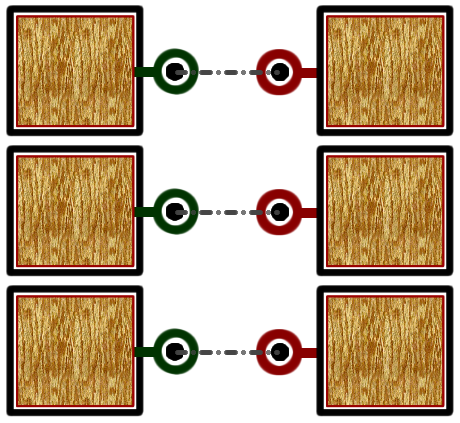
\includegraphics[width=0.25\textwidth]{comm_11.png}
}
\hspace{0.05\textwidth}%
\subfloat[][Communication 1 to N]{%
	\label{subfig:comm_diff}
	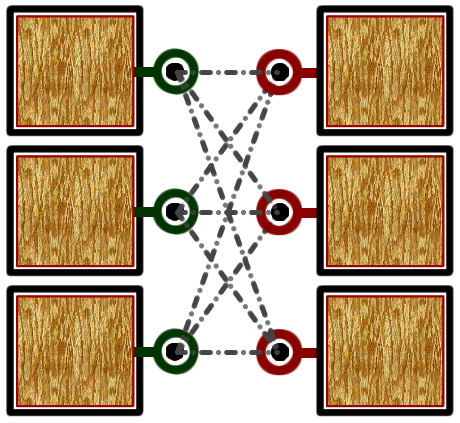
\includegraphics[width=0.25\textwidth]{comm_1n.png}
}
\hspace{0.05\textwidth}%
\subfloat[][Cyclic communication]{%
	\label{subfig:comm_ring}
	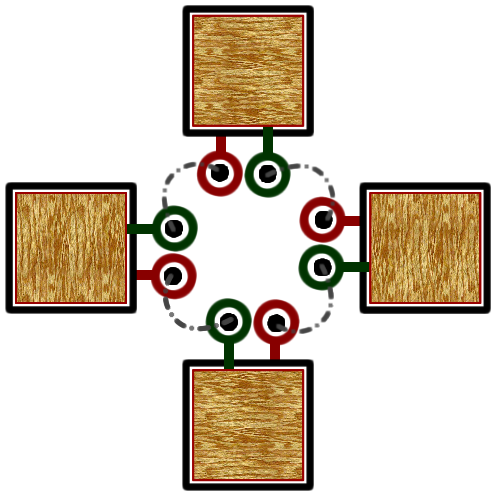
\includegraphics[width=0.25\textwidth]{comm_ring2.png}
}
\caption[]{Graphic representation of communication operators}
\label{fig:comm}
\end{figure}

\poslexample{These operators can be combined beteewn themself to contruct any kind of \comstr. Figure~\ref{fig:ex:comb} shows a simple example combining solvers doubly connected and non connected solvers. Assuming that all solvers $S_i, i\in[1..5]$ have a module $\mathcal{M}$ sent by a send operator, and a \opch{} $\mathcal{CM}$, the corresponding code is the following:
\begin{gather*}
\left[\mathcal{S}_1\cdot\mathcal{M}, \mathcal{S}_2\cdot\mathcal{M}, \mathcal{S}_{3}\cdot\mathcal{M}\right] \onetonsep \left[\mathcal{S}_4\cdot\mathcal{CM}, \mathcal{S}_5\cdot\mathcal{CM}\right]\\
\left[\mathcal{S}_4\cdot\mathcal{M}, \mathcal{S}_5\cdot\mathcal{M}\right] \onetoonesep \left[\mathcal{S}_1\cdot\mathcal{CM}, \mathcal{S}_{3}\cdot\mathcal{CM}\right]\\
\left[\mathcal{S}_6\right]\\
\left[\mathcal{S}_7\right]
\end{gather*}
}

\begin{figure}[h]
\centering
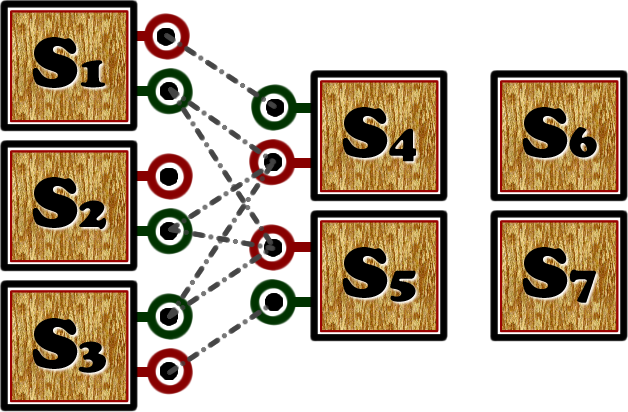
\includegraphics[width=0.35\textwidth]{ex_comb.png}
\caption[]{Graphic representation of communication operators}
\label{fig:ex:comb}
\end{figure}

\separation

%When we apply a connection operator $\circled{op}$ between a \jacks{} list $\mathcal{J}$ and a \outlets{} list $\mathcal{O}$, internally we are assigning an \textit{computation unit} (typically a thread) to each solver that we declare in each list. This assignment receives the name of \textit{Solver Scheduling}. Before running the \soset{}, this \textit{computation unit} is just an integer $\tau \in [0..N]$ identifying uniquely each of the solvers. When the \soset{} is launched, the solver with the identifier $\tau$ runs inside the computation unit $\tau$. This identifier assignation remains independent of the real availability of resources of computation. It just takes into account the user declaration. This means that, if the user declares 30 solvers (15 senders and 15 receivers) and the \soset{} is launched using 20 cores, only the first 20 solvers will be executed, and in consequence, there will be 10 solvers sending information to nowhere. Users should take this into account when declaring the \soset.

The connection process depends on the applied connection operator. In each case the goal is to assign, to the sending operator ($\senddataop{.}$ or $\sendmoduleop{.}$) inside the \as{}, the identifier of the solver (or solvers, depending on the connection operator) where the information will be sent. Algorithm~\ref{algo:connecting} presents the connection process.

\incmargin{1.4em}
\linesnumbered
\begin{algorithm}[H]
\dontprintsemicolon
\SetLine
\SetKwFor{While}{while}{do}{end}
\SetKwData{Jacks}{$\mathcal{J}$}
\SetKwData{Outlets}{$\mathcal{O}$}
\SetKwData{SS}{$S$}
\SetKwData{SSjack}{$S_{jack}$}
\SetKwData{RR}{$R$}
\SetKwData{RRoutlet}{$R_{outlet}$}
\SetKwData{RRid}{$R_{id}$}
\SetKwFunction{GetSolver}{GetSolverFromConnector}
\SetKwFunction{GetNext}{GetNext}
\SetKwFunction{Sched}{Schedule}
\SetKwFunction{Root}{root}
\SetKwFunction{Connect}{Connect}
\SetKwInOut{Input}{input}
\SetKwInOut{Output}{output}
\SetKw{KwTo}{int}

\Input{\Jacks list of \jacks{}, \\ \Outlets list of \outlets}
%\Output{\Q = $\left\{Q_i\right\}_{i=1\dots K}$: $K$ subsets of \Uni}
%\BlankLine
\While{no available jacks or outlets remain}{ %\nllabel{paso_condicion}
	\SSjack	$\leftarrow$ \GetNext{\Jacks}\;
	\RRoutlet $\leftarrow$ \GetNext{\Outlets}\;
	\SS $\leftarrow$ \GetSolver{\SSjack}\;	
	\RR $\leftarrow$ \GetSolver{\RRoutlet}\;
	%\Sched{\SS}\;
	%\RRid $\leftarrow$ \Sched{\RR}\;
	\Connect{\Root{\SS},\SSjack, \RR} %\RRid} %\label{step2} \tcc{It also removes the returned element}
}
\caption{Connection main algorithm}\label{algo:connecting}
\end{algorithm}

In Algorithm~\ref{algo:connecting}:
\begin{itemize}
\item \texttt{GetNext($\dots$)} returns the next available solver-jack (or solver-outlet) in the list, depending on the connection operator, e.g., for the connection operator One-to-N, each \jack{} in $\mathcal{J}$ must be connected with each \outlet{} in $\mathcal{O}$.
\item \texttt{GetSolverFromConnector($\dots$)} returns the solver name given a connector declaration.
%\item \texttt{Schedule($\dots$)} schedules a solver and returns its identifier.
\item \texttt{Root($\dots$)} returns the {\it root} \cm{} of a solver.
\item \texttt{Connect($\dots$)} %is presented in Algorithm~\ref{algo:connect}. It 
searches the \om{} $S_{jack}$ recursively inside the {\it root} \cm{} of $S$ and places the identifier $R_{id}$ into its list of destination solvers.
\end{itemize}

\poslexample{Let us suppose that we have declared two solvers $S$ and $Z$, both implementing the \as{} in Algorithm~\ref{algo:as_example}, so they can be either sender or receiver. The following code connects them using the operator {\bf 1~to~N}:
$$\left[S\cdot A\right] \onetonsep \left[Z\cdot C.M.\right]$$
If the operator {\bf 1~to~N} is used with only with one solver in each list, the operation is equivalent to applying the operator {\bf 1~to~1}. However, to obtain a communication strategy like the one showed in Figure~\ref{subfig:comm_diff}, six solvers (three senders and three receivers) have to be declared to be able to apply the following operation:
$$\left[S_1\cdot A, S_2\cdot A, S_3\cdot A\right]\onetonsep \left[Z_1\cdot C.M., Z_2\cdot C.M., Z_3\cdot C.M.\right]$$
\posl{} provides a mechanism to make this easier, through two {\it syntactic sugars} explained below.
}

%\subsection{Solver namespace expansion}
\separation

One of the goals of \posl{} is to provide a way to declare sets of solvers to be executed in parallel easily. For that reason, \posl{} provides two syntactic sugars %forms of namespace expansion, 
in order to create sets of solvers using already declared ones:
\begin{enumerate}
\item Using an integer to denote how many times a solver name will appear in the declaration.
\item Using an integer to denote how many times the connection will be repeated in the declaration.
\end{enumerate}

The following example explains clearly these syntactic sugars:

%\textbf{Solver name expansion - } Uses an integer $K$ to denote how many times the solver name $S$ will appear in the declaration. $\left[\dots S_i\cdot\mathcal{M}(K),\dots\right]$ expands as $\left[\dots S_i\cdot\mathcal{M}, S_i^2\cdot\mathcal{M},\dots S_i^K\cdot\mathcal{M}\dots\right]$\\
%and all new solvers $S_i^j, j\in [2..K]$ are created using the same solver declaration of solver $S_i$.

%\textbf{Connection declaration expansion - } Uses an integer $K$ to denote how many times the connection will be repeated in the declaration. Let 
%\begin{inparaenum}[a)]
%\item $\left[\mathcal{S}_1\cdot\mathcal{M}_1,\dots,\mathcal{S}_{N}\cdot\mathcal{M}_{N}\right]$ and 
%\item $\left[\mathcal{R}_1\cdot\mathcal{CM}_1,\dots,\mathcal{R}_{M}\cdot\mathcal{CM}_{M}\right]$ be the list of \jacks{} and \outlets, respectively, and
%\item $\circled{op}$ a connection operator.
%\end{inparaenum} Then $$\left[\mathcal{S}_1\cdot\mathcal{M}_1,\dots,\mathcal{S}_{N}\cdot\mathcal{M}_{N}\right] \poslop{op} \left[\mathcal{R}_1\cdot\mathcal{CM}_1,\dots,\mathcal{R}_{M}\cdot\mathcal{CM}_{M}\right]K$$ expands as
%
%\begin{align*}
%\left[\mathcal{S}_1\cdot\mathcal{M}_1,\dots,\mathcal{S}_{N}\cdot\mathcal{M}_{N}\right] &\poslop{op} \left[\mathcal{R}_1\cdot\mathcal{CM}_1,\dots,\mathcal{R}_{M}\cdot\mathcal{CM}_{M}\right]\\
%\left[\mathcal{S}_1^2\cdot\mathcal{M}_1,\dots,\mathcal{S}_{N}^2\cdot\mathcal{M}_{N}\right] &\poslop{op} \left[\mathcal{R}_1^2\cdot\mathcal{CM}_1,\dots,\mathcal{R}_{M}^2\cdot\mathcal{CM}_{M}\right]\\
%&\dots\\
%\left[\mathcal{S}_1^K\cdot\mathcal{M}_1,\dots,\mathcal{S}_{N}^K\cdot\mathcal{M}_{N}\right] &\poslop{op} \left[\mathcal{R}_1^K\cdot\mathcal{CM}_1,\dots,\mathcal{R}_{M}^K\cdot\mathcal{CM}_{M}\right]\\
%\end{align*}
%and all new solvers $S_i^k, i\in[1..N]$ and $R_j^k,j\in [1..M]$, $k\in[2..K]$, are created using the same solver declaration of solvers $S_i$ and $R_j$, respectively.

\poslexample{Suppose that I have created  solvers $S$ and $Z$ mentioned in the previews example. As a communication strategy, I want to connect them through the operator {\bf 1~to~N}, using $S$ as sender and $Z$ as receiver. Then,  %using \textbf{namespace expansions}, 
we need to declare how many solvers I want to connect. Algorithm~\ref{algo:comm_str_ex} shows the desired communication strategy. Notice in this example that the connection operation is affected also by the number $2$ at the end of the line. %, as {\bf connection declaration expansion}. 
In that sense, and supposing that 12 units of computation are available, a \soset{} working on parallel following the topology described in Figure~\ref{fig:ex_conn} can be obtained.}

\begin{algorithm}[H]
\dontprintsemicolon
\SetNoline
%\myproc{
[ S$\cdot A$ (3) ] $\onetonsep$ [ Z$\cdot C.M.$ (3) ] 2 ;
\caption{A communication strategy}\label{algo:comm_str_ex}
\end{algorithm}

\begin{figure}[h]
	\centering	
	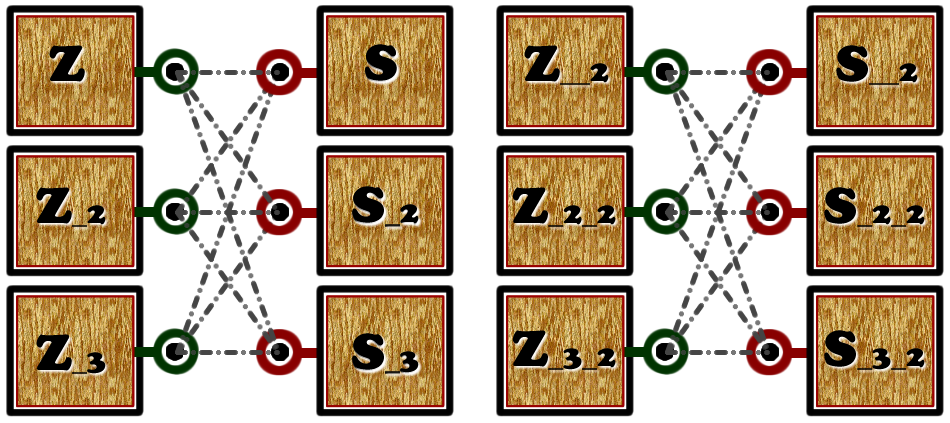
\includegraphics[width=0.6\linewidth]{ex_top.png}
	\caption{An example of connection strategy for 12 units of computation}\label{fig:ex_conn}
\end{figure}

\section{Summarize}
\label{sec:posl_zum}

In this chapter \posl{} have been formally presented, as a Parallel--Oriented Solver Language to build meta-heuristic-based solver to solve \CSPs{}. This language provides a set of \oms{} useful to solve a wide range of constrained problems. It is also possible to create new ones, through the low-level framework in C++ programming language. \posl{} also provides a set of \opchs{}, essential features to share information between solvers.

One of the most important advantages of \posl{} is the possibility of creating \ass{} using an operator-based language, that remains independent from used \bothmodules{}. That is the reason why it is possible to create many different solvers using the same solution strategy (the \as) by instantiating it with different modules (\bothmodules). It is also possible to create different \comstrs{} by using {\it connection operators} that \posl{} provides.

In the next chapter, a detailed study of various communicating and non-communicating strategies is presented, using some \CSPs{} as benchmarks. In this study, is showed the efficacy of \posl{} to analyze quickly and easily these strategies.
%\part{Study and evaluation of \posl}
%\chapter{Experiments design and results}
\label{chap:expe}
\textit{In this Chapter I expose all details about the evaluation process of \posl{}, i.e., all experiments I perform. For each benchmark, I explain used strategies in the evaluation process and the used environments were the runs were performed (\textit{Curiosiphi} server). %, and eventually \textit{Grid5000}). 
I describe all the experiments and I expose a complete analysis of the obtained result.}
\vfill
\minitoc
\newpage

In this chapter I illustrate and analyze the versatility of \posl{} studying different ways to solve constraint problems based on local search meta-heuristics. 
I have chosen the \sgp, the \nqp, the \carrp{} and the \grp{} as benchmarks since they are challenging yet differently structured problems. In this Chapter I present formally each benchmark, I explain the structure of \posl's solvers that I have generated for experiments and present a detailed analysis of obtained results.

The experiments\footnote{\posl{} source code is available on GitHub:\href{https://github.com/alejandro-reyesamaro/POSL}{https://github.com/alejandro-reyesamaro/POSL}} 
were performed on an Intel\R{} Xeon\TM{} E5-2680 v2, 10$\times$4 cores, 2.80GHz. This server is called \textit{Coriosiphi} and is located at \textit{Laboratoire d'Informatique de Nantes Atlantique}, at the University of Nantes. Showed results are the means of 30 runs for each setup, presented in columns labeled {\bf T}, corresponding to the run-time in seconds, and {\bf It.} corresponding to the number of iterations; and their respective standard deviations ({\bf T(sd)} and {\bf It.(sd)}). In some tables, the column labeled \textbf{\% success} indicates the percentage of solvers finding a solution before reaching a time--out (5 minutes).

\modified{The experiments in this Chapter are multi-walk runs}. Parallel experiments use 40 cores for all problem instances. It is important to point out that \posl{} is not designed to obtain the best results in terms of performance, but to give the possibility of rapidly prototyping and studying different cooperative or non cooperative search strategies.

\modified{All benchmarks were coded using the \posl{} low-level framework in C++.}

\modified{First results using \posl{} to solve} constraint problems were published in \cite{Reyes-amaro} were we used \posl{} to solve the \sgp{} and study some communication strategies. It was the first version of \posl{}, therefore it was able to solve only relatively easy instances. However, the efficacy of the communication was showed using this tool.

\modified{With the next and more optimized version of \posl{}, I decide to start to perform more detailed studies using the benchmark mentioned before and some others.}

\section{Solving the \sgp}
\label{sec:golfers}

In this section I present the performed study using \sgp{} (\SGP) as a benchmark. The \commstr{} analyzed here consists in applying a mechanism of cost descending acceleration, exchanging the current configuration between two solvers with different characteristics. Final obtained results show that this \commstr{} works pretty well for this problem.

\subsection{Problem definition}

The \sgp{} (\SGP) consists in scheduling $g\times p$ golfers into $g$ groups of $p$ players every week for $w$ weeks, such that two players play in the same group at most once. An instance of this problem can be represented by the triple $g-p-w$. This problem, and other closely related problems, arise in many practical applications such as encoding, encryption, and covering problems~\cite{Lardeux2014}. Its structure is very attractive, because it is very similar to other problems, like \textit{Kirkman's Schoolgirl Problem} and the \textit{Steiner Triple System}. %, so efficient modules to solve a broad range of problems can be built.

The cost function for this benchmark was implemented making an efficient use of the stored information about the cost of the previews configuration. Using integers to work with bit-flags, a table to store the information about the partners of each player in each week can be filled in $O\left(p^2\cdot g \cdot w\right)$. So, if a configuration has $n = (p\cdot g \cdot w)$ elements, this table can be filled in $O\left(p\cdot n\right)$. This table is filled from scratch only one time in the search process (I explain in the next section why). Then, every cost of a new configuration, is calculated based on this information and the performed changes between the new configuration and the stored one. This relative cost is calculated in $O\left(c\cdot g\right)$, where $c$ is the number of performed changed in the new configuration with respect to the stored one.

\subsection{Experiment design and results}

Here, I present the \as{} designed for this problem as well as concrete \oms{} composing the different solvers I have tested:

\begin{enumerate}
	\item Generation abstract module $I$:
	\subitem $I_{BP}$: Returns a random configuration $s$, respecting the structure of the problem, {\it i.e.}, the configuration is a set of $w$ permutations of the vector $[1..n]$, where $n=g\times p$.
	\item Neighborhood abstract modules $V$:
	\subitem $V_{std}$: Given a configuration, returns the neighborhood $\mathcal{V}\left(s\right)$ swapping players among groups.
	\subitem $V_{BAS}$: Given a configuration, returns the neighborhood $\mathcal{V}\left(s\right)$ swapping the most culprit player with other players from the same week. It is based on the {\it Adaptive Search} algorithm.
	\subitem $V_{BP}(p)$: Given a configuration, returns the neighborhood $\mathcal{V}\left(s\right)$ by swapping the most culprit player with other players in the same week, for all $p$ randomly selected weeks.
	\item Selection abstract modules $S$:
	\subitem $S_{first}$: Given a neighborhood, selects the first configuration $s' \in V\left(s\right)$ improving the current cost and returns it together with the current one into the pair $\left(s', s\right)$.
	\subitem $S_{best}$: Given a neighborhood, selects the best configuration $s' \in V\left(s\right)$ improving the current cost and returns it together with the current one into the pair $\left(s', s\right)$.
	\subitem $S_{rand}$: Given a neighborhood, selects randomly a configuration $s' \in V\left(s\right)$ and returns it together with the current one, into the pair $\left(s', s\right)$.
	\item Acceptance abstract module $A$:
	\subitem $A_{AI}$: Given a pair $\left(s', s\right)$, returns always the configuration $s'$
\end{enumerate}

These concrete modules are very useful and can be reused to solve tournament-like problems like \textit{Sports Tournament Scheduling}, \textit{Kirkman's Schoolgirl} and the \textit{Steiner Triple System} problems.

In a first stage of the experiments I use the operator-based language provided by \posl{} to build and test many different non communicating strategies. The goal is to select the best concrete modules to run tests performing communication. A very first experiment was performed to select the best neighborhood function to solve the problem, comparing a basic solver using $V_{std}$; a new solver using $V_{BAS}$; and a combination of $V_{std}$ and $V_{BAS}$ by applying the operator $\circled{$\rho$}$, already introduced in the previous chapter. Algorithms~\ref{as:golfers10-10-3} and \ref{as:golfers_rho} present solvers for each case, respectively.

\begin{algorithm}[t]
\dontprintsemicolon
\SetNoline
\SetKwProg{myproc}{\tet{\bf abstract solver}}{\tet{\bf begin}}{\tet{\bf end}}
\myproc{as\_simple \tcp*{{\sc Itr} $\rightarrow$ number of iterations}
	\tet{\bf computation} : $I, V, S, A$\;}{
	\whileinline{$\left(\textbf{\Iter < } K_1\right)$}{%M_1^a \circled{$\rho$} M_1^b
		$I \poslop{\mapsto}$
		\whileinline{$\left(\textbf{\Iter \% } K_2\right)$}{$\left[V \poslop{\mapsto} S \poslop{\mapsto} A\right]$}
	}	
}
\tet{\bf solver} \solverposl{Std} \tet{\bf implements} as\_simple\;
\algoindent \tet{\bf computation} : $I_{BP}, V_{std}, S_{best}, A_{AI}$ \;
\tet{\bf solver} \solverposl{AS} \tet{\bf implements} as\_simple\;
\algoindent \tet{\bf computation} : $I_{BP}, V_{BAS}, S_{best}, A_{AI}$ \; 
%\tet{\bf connection}: $CM_{last}$\;
\caption{Simple solvers for \SGP}\label{as:golfers10-10-3}
\end{algorithm}

\begin{algorithm}[H]
\dontprintsemicolon
\SetNoline
\SetKwProg{myproc}{\tet{\bf abstract solver}}{\tet{\bf begin}}{\tet{\bf end}}
\myproc{as\_rho \tcp*{{\sc Itr} $\rightarrow$ number of iterations}
	\tet{\bf computation} : $I, V_1, V_2, S, A$\;}{
	\whileinline{$\left(\textbf{\Iter < } K_1\right)$}{%M_1^a \circled{$\rho$} M_1^b
		$I \poslop{\mapsto}$
		\whileinline{$\left(\textbf{\Iter \% } K_2\right)$}{$\left[\left[V_1 \poslop{\rho} V_2\right] \poslop{\mapsto} S \poslop{\mapsto} A\right]$}
	}	
}
\tet{\bf solver} \solverposl{rho} \tet{\bf implements} as\_rho\;
\algoindent \tet{\bf computation} : $I_{BP}, V_{std}, V_{BAS}, S_{best}, A_{AI}$ \;
\caption{Solvers combining neighborhood functions using operator {\it RHO}}\label{as:golfers_rho}
\end{algorithm}

\begin{table}
\centering 
\renewcommand{\arraystretch}{1}
\begin{tabular}{p{4cm}|R{1.3cm}R{1.3cm}R{1.3cm}R{1.3cm}}
\hline
{\bf Solver} & T & T(sd) & It. & It.(sd) \\
\hline
%\hline
\texttt{\solverposl{AS}} & \good{\bf 1.06} & 0.79 & 352 & 268 \\		
\texttt{\solverposl{rho}} & 41.53 & 26.00 & 147 & 72\\
%Std $\circled{$\cup$}$ AS & 59.65 & 55.01 & 198 & 110\\
\texttt{\solverposl{Std}} & 87.90 & 41.96 & 146 & 58 \\
\hline
\end{tabular}
\caption{\sg: Instance 10--10--3 in parallel}
\label{tab:golfers10-10-3}
\end{table}

Results in Table~\ref{tab:golfers10-10-3} are not surprising. The neighborhood module $V_{BAS}$ is based on the {\it Adaptive Search} algorithm, which has shown very good results \cite{Diaz}. %It selects the variable (player) contributing the most to the cost and permutes its value with the others variables (players) for all groups, every week.
It selects the most culprit variable (i.e., a player), that is, the variable the most responsible for constraints violation. Then, it permutes this variable value with the value of each other variable, in all groups and all weeks. Each permutation gives a neighbor of the current configuration. $V_{Std}$ uses no additional information, so it performs every possible swap between two players in different groups, every week. It means that this neighborhood is $g\times p$ times bigger than the previous one, with $g$ the number of groups and $p$ the number of players per group. 
It allows for more organized search because the set of neighbors is pseudo-deterministic, i.e., the construction criteria is always the same but the order of the configuration is random. On the other hand, {\it Adaptive Search} neighborhood function takes random decisions more frequently, and the order of the configurations is random as well. We also tested a solver with combining these modules using the $\circled{$\rho$}$ operators. This operator executes its first or second parameter depending on a given probability $\rho$. This combination spent more time searching the best configuration among the neighborhood, although with a lower number of iterations than $V_{BAS}$. The $V_{BAS}$ neighborhood function being clearly faster, we have chosen it for our experiments, even if it shown a more spread standard deviation: 0.75 for \solverposl{AS} versus 0.62 for \solverposl{Std}, considering the ratio $\tfrac{T(sd)}{T}$.

\separation

Once the neighborhood \om{} has been selected, I have focused the experiment on choosing the best {\it selection} \om. Solvers mentioned above were too slow to solve instances of the problem with more than three weeks: they were very often trapped into local minima. For that reason, another solver implementing the \as{} described in Algorithm~\ref{as:golfers_b001} have been created, using $V_{BAS}$ and combining $S_{best}$ and $S_{rand}$: it tries a number of times to improve the cost, and if it is not possible, it picks a random neighbor for the next iteration. We also compared the $S_{first}$ and $S_{best}$ selection modules. The \om{} $S_{best}$ selects the best configuration inside the neighborhood. It did not only spend more time searching a better configuration, but also is was more sensitive to become trapped into local minima. The second \om{} $S_{first}$ selects the first configuration inside the neighborhood improving the current cost. Using this module, solvers favor exploration over intensification and of course spend clearly less time searching into the neighborhood. 

\begin{algorithm}[H]
\dontprintsemicolon
\SetNoline
\SetKwProg{myproc}{\tet{\bf abstract solver}}{\tet{\bf begin}}{\tet{\bf end}}
\myproc{as\_eager \tcp*{{\sc Itr} $\rightarrow$ number of iterations}
	\tet{\bf computation} : $I, V, S_1, S_2, A$\;}{
	\whileinline{$\left(\textbf{\Iter < } K_1\right)$}{%M_1^a \circled{$\rho$} M_1^b
		$I \poslop{\mapsto}$
		\whileinline{$\left(\textbf{\Iter \% } K_2\right)$}{$\left[V \poslop{\mapsto} \left[S_1 \poslopcond{\Sci < K_3} S_2\right] \poslop{\mapsto} A\right]$}
	}
}
\tet{\bf solver} \solverposl{best} \tet{\bf implements} as\_eager\;
\algoindent \tet{\bf computation} : $I_{BP}, V_{std}, V_{BAS}, S_{best}, S_{rand}, A_{AI}$ \;
\tet{\bf solver} \solverposl{first} \tet{\bf implements} as\_eager\;
\algoindent \tet{\bf computation} : $I_{BP}, V_{std}, V_{BAS}, S_{first}, S_{rand}, A_{AI}$ \;
\caption{Solver for \SGP{} to scape from local minima}\label{as:golfers_b001}
\end{algorithm}

\begin{table}
\captionsetup{belowskip=6pt,aboveskip=6pt}
\centering 
\renewcommand{\arraystretch}{1}
\begin{tabular}{p{2cm}|R{1cm}R{1cm}R{1cm}R{1.2cm}|R{1cm}R{1cm}R{1cm}R{1.2cm}}
	\hline %\noalign{\smallskip}	
	\multirow{2}{*}{\footnotesize{\centering {\bf Instance}}} & 
	\multicolumn{4}{c|}{Best improvement} & 
	\multicolumn{4}{c}{First improvement}\\
	\cline{2-9} %\cline{3-8}
	& T & T(sd) & It. & It.(sd) & T & T(sd) & It. & It.(sd) \\
	\hline
	%\hline
	5--3--7 & 0.45 & 0.70 & 406 & 726 & 0.23 & 0.14 & 142 & 67\\
	8--4--7 & 0.37 & 0.11 & 68 & 13 & 0.28 & 0.07 & 93 & 13\\	
	9--4--8 & 0.87 & 0.13 & 95 & 17 & 0.60 & 0.16 & 139 & 18 \\
	\hline
\end{tabular}
\caption{\sg: comparing selection functions in parallel}
\label{tab:golfersB001}
\end{table}

\begin{table}[h]
\centering
\renewcommand{\arraystretch}{1}
\begin{tabular}{p{1.5cm}|R{1.5cm}R{1.5cm}R{1.5cm}R{1.5cm}}
\hline
{\bf Instance} & T & T(sd) & It. & It.(sd)\\
\hline
%\hline
5--3--7 & 1.25 & 1.05 & 2,907 & 2,414 \\
8--4--7 & 0.60 & 0.33 & 338 & 171 \\
9--4--8 & 1.04 & 0.72 & 346 & 193\\
\hline
\end{tabular}
\caption{\sg: a single sequential solver using first improvement}
\label{tab:golfers_seq}
\end{table}

Tables~\ref{tab:golfersB001} and \ref{tab:golfers_seq} present results of this experiment, showing that a local exploration-oriented strategy is better for the \SGP. If we compare results of Tables~\ref{tab:golfersB001} \ref{tab:golfers_seq} with respect to the standard deviation, we can some gains in robustness with parallelism. The spread in the running times and iterations for the instance 5--3--7 is 24\% lower (0.84 sequentially versus 0.60 in parallel), for 8--4--7 is 30\% lower (0.55 sequentially versus 0.25 in parallel) and for 9--4--8 (the hardest one) is 43\% lower (0.69 sequentially versus 0.26 in parallel), using the same ratio $\tfrac{T(sd)}{T}$).

\separation

The conclusion of the last experiment was that the best solver to solve \SGP{} using \posl{} is the one using a neighborhood \om{} based on {\it Adaptive Search} algorithm ($V_{BAS}$) and a selection \om{} selecting the first configuration improving the cost. Using this solver as a base, the next step was to design a simple communication strategy where the shared information is the current configuration. Algorithms~\ref{as:golfers_sender}~and~\ref{as:golfers_receiver} show that the communication is performed while applying the acceptance criterion of the new configuration for the next iteration. Here, receiver solvers receive a configuration from a sender solver, and match it with their current configuration. Then, the configuration with the lowest global cost is selected. This operation is coded using the \textit{minimum} operator $\poslop{m}$ in Algorithm~\ref{as:golfers_receiver}. This way, the receiver solver continues the search from a more promising place into de search space. Different communication strategies were designed, either executing a full connected solvers set, or a tuned combination of connected and unconnected solvers. Between connected solvers, two different connections operations were applied: connecting each sender solver with one receiver solver (\oneTone), or connecting each sender solver with all receiver solvers (\oneTn). The code for the different \commstrs{} are presented in Algorithms~\ref{comm:golfers_1_1-1} to \ref{comm:golfers_1_1-n_25}.

\begin{algorithm}
\dontprintsemicolon
\SetNoline
\SetKwProg{myproc}{\tet{\bf abstract solver}}{\tet{\bf begin}}{\tet{\bf end}}
\myproc{as\_eager\_sender \tcp*{{\sc Itr} $\rightarrow$ number of iterations}
	\tet{\bf computation} : $I, V, S_1, S_2, A$\tcp*{{\sc Sci} $\rightarrow$ number of iterations with the same cost}}{%	
	\whileinline{$\left(\textbf{\Iter < } K_1\right)$}{
		$I \poslop{\mapsto}$
		\whileinline{$\left(\textbf{\Iter \% } K_2\right)$}{$\left[V \poslop{\mapsto} \left[S_1 \poslopcond{\Sci < K_3} S_2\right] \poslop{\mapsto} \llparenthesis A \rrparenthesis^o\right]$}
	}
}
\tet{\bf solver} \solverposl{sender} \tet{\bf implements} as\_eager\_sender\;
\algoindent \tet{\bf computation} : $I_{BP}, V_{BAS}, S_{first}, S_{rand}, A_{AI}$ \;
\caption{Communicating \as{} for \SGP{} (sender)}\label{as:golfers_sender}
\end{algorithm}

\begin{algorithm}
\dontprintsemicolon
\SetNoline
\SetKwProg{myproc}{\tet{\bf abstract solver}}{\tet{\bf begin}}{\tet{\bf end}}
\myproc{as\_eager\_receiver \tcp*{{\sc Itr} $\rightarrow$ number of iterations}
	\tet{\bf computation} : $I, V, S_1, S_2, A$\tcp*{{\sc Sci} $\rightarrow$ number of iterations with the same cost}
	\tet{\bf communication} : $C.M.$\;}{%	
	\While{$\left(\textbf{\Iter < } K_1\right)$}{%M_1^a \circled{$\rho$} M_1^b
		$I \poslop{\mapsto}$
		\whileinline{$\left(\textbf{\Iter \% } K_2\right)$}{
			$ V \poslop{\mapsto} \left[S_1 \poslopcond{\Sci < K_3} S_2\right] \poslop{\mapsto} \left[A \poslop{m} C.M.\right]$
		}
	}
}
\tet{\bf solver} \solverposl{receiver} \tet{\bf implements} as\_eager\_receiver\;
\algoindent \tet{\bf computation} : $I_{BP}, V_{BAS}, S_{first}, S_{rand}, A_{AI}$ \;
\algoindent \tet{\bf communication} : $CM_{last}$
\caption{Communicating \as{} for \SGP{} (receiver)}\label{as:golfers_receiver}
\end{algorithm}

\begin{algorithm}
\dontprintsemicolon
\SetNoline
$\left[\eqsolverposl{sender}\cdot A\right] \onetoone \left[\eqsolverposl{receiver}\cdot C.M.\right]20;$
\caption{Communication strategy \oneTone{} 100\%}\label{comm:golfers_1_1-1}
\end{algorithm}

\begin{algorithm}
\dontprintsemicolon
\SetNoline
$\left[\eqsolverposl{sender}\cdot A(20)\right] \oneton \left[\eqsolverposl{receiver}\cdot C.M.(20)\right];$
\caption{Communication strategy \oneTn{} 100\%}\label{comm:golfers_1_1-n}
\end{algorithm}

\begin{algorithm}
\dontprintsemicolon
\SetNoline
$\left[\eqsolverposl{sender}\cdot A\right] \onetoone \left[\eqsolverposl{receiver}\cdot C.M.\right]10;$\;
$\left[\eqsolverposl{first}\right]20;$
\caption{Communication strategy \oneTone{} 50\%}\label{comm:golfers_1_1-1_50}
\end{algorithm}

\begin{algorithm}
\dontprintsemicolon
\SetNoline
$\left[\eqsolverposl{sender}\cdot A(10)\right] \oneton \left[\eqsolverposl{receiver}\cdot C.M.(10)\right];$\;
$\left[\eqsolverposl{first}\right]20;$
\caption{Communication strategy \oneTn{} 50\%}\label{comm:golfers_1_1-n_50}
\end{algorithm}

\begin{algorithm}
\dontprintsemicolon
\SetNoline
$\left[\eqsolverposl{sender}\cdot A\right] \onetoone \left[\eqsolverposl{receiver}\cdot C.M.\right]5;$\;
$\left[\eqsolverposl{first}\right]30;$
\caption{Communication strategy \oneTone{} 25\%}\label{comm:golfers_1_1-1_25}
\end{algorithm}

\begin{algorithm}
\dontprintsemicolon
\SetNoline
$\left[\eqsolverposl{sender}\cdot A(5)\right] \oneton \left[\eqsolverposl{receiver}\cdot C.M.(5)\right];$\;
$\left[\eqsolverposl{first}\right]30;$
\caption{Communication strategy \oneTn{} 25\%}\label{comm:golfers_1_1-n_25}
\end{algorithm}

In Algorithm~\ref{as:golfers_receiver}, the abstract \opch{} $C.M.$ was instantiated with the concrete \opch{} $CM_{last}$, which takes into account the last received configuration at the time of its execution.

Each time a \posl{} meta-solver is launched, many independent search solvers are executed. We call "good" configuration a configuration with the lowest cost within the current configuration neighborhood and with a cost strictly lesser than the current one. Once a good configuration is found in a sender solver, it is transmitted to the receiver one. At this moment, if the information is accepted, there are some solvers searching in the same subset of the search space, and the search process becomes more exploitation--oriented. This can be problematic if this process makes solvers converging too often towards local minima. In that case, we waste more than one solver trapped into a local minima: we waste all solvers that have been attracted to this part of the search space because of communications. This phenomenon is avoided through a simple (but effective) play: if a solver is not able to find a better configuration inside the neighborhood (executing $S_{first}$), it selects a random one at the next iteration (executing $S_{rand}$).

In all Algorithms in this section, three parameter can be found:\begin{inparaenum}[1.] \item $K_1$: the maximum number of {\it restarts}, \item $K_2$: the maximum number of iterations in each \textit{restart}, and $K_3$: the maximum number of iterations with the same current cost. \item \end{inparaenum}

After the selection of the proper modules to study different communication strategies, I proceeded to tune these parameter. Only a few runs were necessaries to conclude that the mechanism of using the \om{} $S_{rand}$ to scape from local minima was enough. For that reason, since the solver never perform restarts, the parameter $K_1$ was irrelevant. So the reader can assume $K_1 = 1$ for every experiment.

With the certainty that solvers do not performs restarts during the search process, I select the same value for $K_2 = 5000$ in order to be able to use the same \as{} for all instances.

Finally, in the tuning process of $K_3$, I notice only slightly differences between using the values $5$, $10$, and $15$. So I decided to use $K_3 = 5$.

\begin{table}
	\captionsetup{belowskip=6pt,aboveskip=6pt}
	\centering 
	\renewcommand{\arraystretch}{1}
		\begin{tabular}{p{2cm}|R{1cm}R{1cm}R{1cm}R{1.2cm}|R{1cm}R{1cm}R{1cm}R{1.2cm}}
			\hline 	
			\multirow{2}{*}{\centering {\bf Instance}} & \multicolumn{4}{c}{Communication 1 to 1} & \multicolumn{4}{c}{Communication 1 to N}\\
			\cline{2-9}
			& T & T(sd) & It. & It.(sd) & T & T(sd) & It. & It.(sd) \\
			\hline
			%\hline
			5--3--7 & 0.20 & 0.20 & 165 & 110 & 0.20 & 0.17 & 144 & 108\\
			8--4--7 & 0.27 & 0.09 & 88 & 28 & 0.24 & 0.05 & 95 & 12\\
			9--4--8 & 0.52 & 0.14 & 117 & 25 & 0.55 & 0.14 & 126 & 20\\
%			11--7--5 & 1.76 & 0.41 & 214 & 44 & \good{1.62} & 0.34 & \good{202} & 30\\
			\hline
		\end{tabular}
	\caption{\sg: 100\% of communicating solvers}
	\label{tab:golfersB001comm100}
\end{table}

\begin{table}
	\captionsetup{belowskip=6pt,aboveskip=6pt}
	\centering 
	\renewcommand{\arraystretch}{1}
		\begin{tabular}{p{2cm}|R{1cm}R{1cm}R{1cm}R{1.2cm}|R{1cm}R{1cm}R{1cm}R{1.2cm}}
			\hline 	
			\multirow{2}{*}{\centering {\bf Instance}} & \multicolumn{4}{c}{Communication 1 to 1} & \multicolumn{4}{c}{Communication 1 to N}\\
			\cline{2-9}
			& T & T(sd) & It. & It.(sd) & T & T(sd) & It. & It.(sd) \\
			\hline
			%\hline
			5--3--7 & 0.18 & 0.13 & 125 & 88 & 0.17 & 0.12 & 139 & 81\\
			8--4--7 & 0.21 & 0.06 & 89 & 18 & 0.22 & 0.06 & 90 & 20\\
			9--4--8 & 0.49 & 0.11 & 119 & 24 & 0.51 & 0.15 & 124 & 21 \\
%			11--7--5 & 1.81 & 0.40 & 220 & 33 & 1.82 & 0.39 & 222 & 39\\
			\hline
		\end{tabular}
	\caption{\sg: 50\% of communicating solvers}
	\label{tab:golfersB001comm50}
\end{table}

\begin{table}
	\captionsetup{belowskip=6pt,aboveskip=6pt}
	\centering 
	\renewcommand{\arraystretch}{1}
		\begin{tabular}{p{2cm}|R{1cm}R{1cm}R{1cm}R{1.2cm}|R{1cm}R{1cm}R{1cm}R{1.2cm}}
			\hline 	
			\multirow{2}{*}{\centering {\bf Instance}} & \multicolumn{4}{c}{Communication 1 to 1} & \multicolumn{4}{c}{Communication 1 to N}\\
			\cline{2-9}
			& T & T(sd) & It. & It.(sd) & T & T(sd) & It. & It.(sd) \\
			\hline
			%\hline
			5--3--7 & 0.22 & 0.20 & 181 & 130 & 0.23 & 0.16 & 143 & 80\\
			8--4--7 & 0.24 & 0.08 & 95 & 22 & 0.29 & 0.09 & 93 & 12\\
			9--4--8 & 0.55 & 0.14 & 134 & 21 & 0.55 & 0.11 & 130 & 20\\
%			11--7--5 & 1.99 & 0.54 & 242 & 51 & 1.63 & 0.35 & 224 & 28 \\
			\hline
		\end{tabular}
	\caption{\sg: 25\% of communicating solvers}
	\label{tab:golfersB001comm25}
\end{table}

This communication strategy produces some gain in terms of runtime (Table~\ref{tab:golfersB001} with respect to Tables~\ref{tab:golfersB001comm100}, \ref{tab:golfersB001comm50} and \ref{tab:golfersB001comm25}). 
Having many solvers searching in different places of the search space, the probability that one of them reaches a promising place is higher. Then, when a solver finds a good configuration, it can be communicated, and receiving the help of one or more solvers in order to find the solution.
Using this strategy, the spread in the running times and iterations was reduced for the instance 9--4--8 (0.22 using communication \oneTone{} and 50\% of communication solvers), but not for instances 5--3--7 and 8--4--7 (0.70 using communication \oneTn{} and 50\% of communicating solvers, and 0.28 using communication \oneTone{} and 50\% of communicating solvers, respectively).

Other two strategies were analyzed in the resolution of this problem, with no success, both based on the sub-division of the work by weeks, i.e., solvers trying to improve a configuration only working with one or some weeks. To this end two strategies were designed:

\begin{enumerate}[label=\Alph*]
\item \textbf{Circular strategy:} $K$ solvers try to improve a configuration during a during a number of iteration, only working on one week. When no improvement is obtained, the current configuration is communicated to the next solver (circularly), which tries to do the same working on the next week (see Figure~\ref{subfig:golfers_bad_ring}).
\subitem This strategy does not show better results than previews strategies. The reason is because, although the communication in \posl{} is asynchronous, most of the times solvers were trapped waiting for a configuration coming from its neighbor solver.

\item \textbf{Dichotomy strategy:} Solvers are divided by levels. Solvers in level 1, only work on one week, solvers on level 2, only work on 2 consecutive weeks, and so on, until the solver that works on all (except the first one) weeks. Solvers in level 1 improve a configuration during some number of iteration, then this configuration is sent to the corresponding solver. Solvers in level 2 do the same, but working on weeks $k$ to $k+1$. It means that it receives configurations from the solver working on week $k$ and from the solver working on week $k+1$, and sends its configuration to the corresponding solver working on weeks $k$ to $k+3$; and so on. The solver in the last level works on all (except the first one) weeks and receive configuration from the solver working on weeks $2$ to $w/2$ and from the solver working on weeks $w/2+1$ to $w$ (see Figure\ref{subfig:golfers_bad_dic}). We tested this strategy with all possible levels. 
\subitem The goal of this strategy was testing if focused searches rapidly communicated can help at the beginning of the search. However, The failure of this strategy is in the fact that most of the time the sent information arrives to late from the bottom to the top.
\end{enumerate}

\begin{figure}[h]
	\centering
	\subfloat[][]{
		\label{subfig:golfers_bad_ring}
		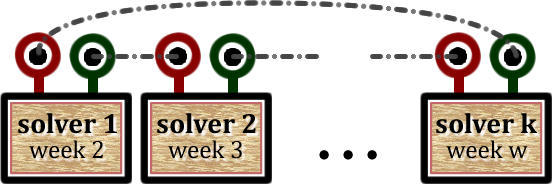
\includegraphics[width=0.45\linewidth]{golfers_ring.png}
	} %\hspace{0.1\linewidth}
	\subfloat[][]{%
		\label{subfig:golfers_bad_dic}
		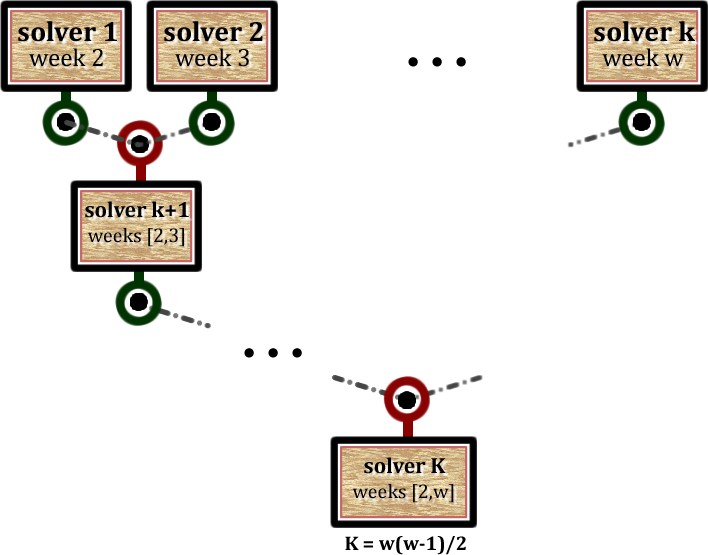
\includegraphics[width=0.45\linewidth]{golfers_dic.png}
	}
	\caption[]{Unsuccessful communication strategies to solve \SGP}
	\label{fig:golfers_bad}
\end{figure}

\separation

One last experiment using this benchmark was implementing a \commstr{} which applies a mechanism of cost descending acceleration, exchanging the current configuration between two solvers with different characteristics. Results show that this \commstr{} works pretty well for this problem.

For this strategy, new solvers were built reusing same \ms{} used for the \commstrs{} exposed before, and another different neighborhood \om{}: $V_{BP}(p)$, which given a configuration, returns the neighborhood $\mathcal{V}\left(s\right)$ by swapping the culprit player chosen for all $p$ randomly selected weeks with other players in the same week. This new solver was called \textit{companion solver}, and it descends quicker the cost of its current solution at the beginning because its neighborhood generates less values, but the convergence is slower and yet not sure. It was combined with the solver similar to the one used for the \commstrs{} exposed before. It was called \textit{standard solver}, and converges in a stable way to the solution. So, the companion solver uses the same neighborhood function that the standard solver, but parametrized in such a way that it builds neighbors only swapping players among two weeks.

The idea of the \commstr{} is to communicate a configuration from the companion solver to the standard solver, to be able to continue the search from a more promising place into de search space. After some iterations, is the standard solver who sends its configuration to the companion solver. The companion solver takes this received configuration and starts its search from it and finds quickly a much better configuration to send to the standard solver again. To force the companion solver to take the received configurations over its own, we use the \textit{not null} operator together with the \opch{} $C.M.$ (Algorithm~\ref{as:golfers_partial}). This process is repeated until a solution is found.

Figure~\ref{fig:solversgolfers} shows standard solver's run versus companion solver's run. In this chart we can see that, at the beginning of the run, found configurations by the companion solver have costs significantly lower than those found by the standard solver. \tet{At the 60-th millisecond} the standard solver current configuration has cost 123, and the companion solver's one, 76. So for example, the communication at this time, can accelerate the process significantly.

\begin{figure}
\centering
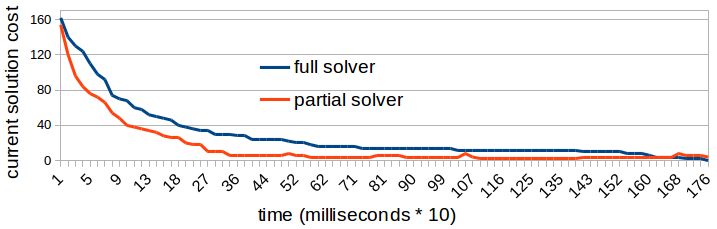
\includegraphics[width=0.9\columnwidth]{graph.png} 
\caption{Companion solver vs. standard solver (solving \sgp)}
\label{fig:solversgolfers}
\end{figure}

\begin{algorithm}
\dontprintsemicolon
\SetNoline
\SetKwProg{myproc}{\tet{\bf abstract solver}}{\tet{\bf begin}}{\tet{\bf end}}
\myproc{as\_standard \;
	\tet{\bf computation} : $I, V, S_1, S_2, A$\;
	\tet{\bf communication} : $C.M.$\;}{%
	$I \poslop{\mapsto}$
	\whileinline{$\left(\textbf{\Iter} < K_1\right)$}{
		$V \poslop{\mapsto} \left[S_1 \poslopcond{\Sci \% K_1} S_1\right] \poslop{\mapsto} \left[C.M. \poslop{m} \llparenthesis A \rrparenthesis^d\right]$		
	}
}
\tet{\bf solver} \solverposl{standard} \tet{\bf implements} as\_standard\;
\algoindent \tet{\bf computation} : $I_{BP}, V_{BAS}, S_{first}, S_{rand}, A_{AI}$ \;
\algoindent \tet{\bf communication} : $CM_{last}$ \;
\caption{Standard solver for \SGP}\label{as:golfers_full}
\end{algorithm}

\begin{algorithm}
\dontprintsemicolon
\SetNoline
\SetKwProg{myproc}{\tet{\bf abstract solver}}{\tet{\bf begin}}{\tet{\bf end}}
\myproc{as\_companion \;
	\tet{\bf computation} : $I, V, S_1, S_2, A$\;
	\tet{\bf communication} : $C.M.$\;}{
	$I \poslop{\mapsto}$
	\whileinline{$\left(\textbf{\Iter} < K_1\right)$}{
		$V \poslop{\mapsto} \left[S_1 \poslopcond{\Sci \% K_1} S_2\right] \poslop{\mapsto} \left[C.M. \poslop{\vee} \llparenthesis A \rrparenthesis^d\right]$		
	}
}
\tet{\bf solver} \solverposl{companion} \tet{\bf implements} as\_companion\;
\algoindent \tet{\bf computation} : $I_{BP}, V_{BP}(2), S_{first}, S_{rand}, A_{AI}$ \;
\algoindent \tet{\bf communication} : $CM_{last}$ \;
\caption{Companion solver for \SGP}\label{as:golfers_partial}
\end{algorithm}

We also design different \commstrs, combining connected and unconnected solvers in different percentages, and applying two different \commopers: \oneTone{} and \oneTn.

This strategy produces some gain in terms of runtime as we can see in Tables~\ref{tab:golfers_v2_1N} and \ref{tab:golfers_v2_11} with respect to Table~\ref{tab:golfersB001}. It produces also more robust results in terms of runtime. The spread of results in iterations show higher variances, because there are included also results of companion solvers, which performs many times more iterations that the standard solvers. The percentage of the receiver solvers that were able to find the solution before the others did, was significant (see Appendix~\ref{app:sgp}, Figures~\ref{barplot:5}, \ref{barplot:8} and \ref{barplot:9}). That shows that the communication played an important role during the search, despite inter--process communication's overheads (reception, information interpretation, making decisions, etc).

The code for the \commstr{} of 100\% of communicating solvers is presented in Algorithm~\ref{comm:golfers_v2_100} and for 50\% of communicating solvers in Algorithm~\ref{comm:golfers_v2_50}. 

\begin{algorithm}[H]
\dontprintsemicolon
\SetNoline
$\left[\eqsolverposl{companion}\cdot A\right] \onetoone \left[\eqsolverposl{standard}\cdot C.M.\right]20;$\;
$\left[\eqsolverposl{standard}\cdot A\right] \onetoone \left[\eqsolverposl{companion}\cdot C.M.\right]20;$
\caption{Companion communication strategy 100\% communication}\label{comm:golfers_v2_100}
\end{algorithm}

\begin{algorithm}[H]
\dontprintsemicolon
\SetNoline
$\left[\eqsolverposl{companion}\cdot A\right] \onetoone \left[\eqsolverposl{standard}\cdot C.M.\right]10;$\;
$\left[\eqsolverposl{standard}\cdot A\right] \onetoone \left[\eqsolverposl{companion}\cdot C.M.\right]10;$\;
$\left[\eqsolverposl{first}\right]20;$\;
\caption{Companion communication strategy 100\% communication}\label{comm:golfers_v2_50}
\end{algorithm}

\begin{table}
\captionsetup{belowskip=6pt,aboveskip=6pt}
\centering 
\renewcommand{\arraystretch}{1}
\resizebox{\columnwidth}{!}{%
\begin{tabular}{p{1.5cm}|R{0.8cm}R{1cm}R{0.6cm}R{1.1cm}|R{0.8cm}R{1cm}R{0.6cm}R{1.1cm}|R{0.8cm}R{1cm}R{0.6cm}R{1.1cm}}
	\hline 	
	\multirow{2}{*}{\centering {\bf Instance}} & \multicolumn{4}{c|}{Comm. \oneTn} & \multicolumn{4}{c}{(Comm. \oneTn)/2} & \multicolumn{4}{c}{(Comm. \oneTn)/4}\\
	\cline{2-13}
	& T & T(sd) & It. & It.(sd) & T & T(sd) & It. & It.(sd) & T & T(sd) & It. & It.(sd) \\
	\hline
	%\hline
	5--3--7 & 0.14 & 0.08 & 102 & 53 & 0.14 & 0.07 & 97 & 73 & 0.12 & 0.08 & 175 & 162 \\
	8--4--7 & 0.30 & 0.13 & 101 & 24 & 0.22 & 0.06 & 92 & 29 & 0.22 & 0.06 & 88 & 45 \\
	9--4--8 & 0.55 & 0.15 & 125 & 20 & 0.53 & 0.14 & 107 & 20 & 0.40 & 0.14 & 101 & 70 \\
	\hline
\end{tabular}
}
\caption{Companion \commstr{} with communication \oneTn}
\label{tab:golfers_v2_1N}
\end{table}

\begin{table}
\captionsetup{belowskip=6pt,aboveskip=6pt}
\centering 
\renewcommand{\arraystretch}{1}
\resizebox{\columnwidth}{!}{%
\begin{tabular}{p{1.5cm}|R{0.8cm}R{1cm}R{0.6cm}R{1.1cm}|R{0.8cm}R{1cm}R{0.6cm}R{1.1cm}|R{0.8cm}R{1cm}R{0.6cm}R{1.1cm}}
	\hline 	
	\multirow{2}{*}{\centering {\bf Instance}} & \multicolumn{4}{c|}{Comm. \oneTone{} (100\%)} & \multicolumn{4}{c|}{Comm. \oneTone{} (50\%)} & \multicolumn{4}{c}{Comm. \oneTone{} (25\%)}\\
	\cline{2-13}
	& T & T(sd) & It. & It.(sd) & T & T(sd) & It. & It.(sd) & T & T(sd) & It. & It.(sd) \\
	\hline
	%\hline
	5--3--7 & 0.10 & 0.05 & 98 & 75 & \good{0.08} & 0.04 & 139 & 122 & 0.11 & 0.05 & 190 & 142 \\
	8--4--7 & \good{0.14} & 0.05 & 100 & 64 & 0.22 & 0.06 & 119 & 74 & 0.21 & 0.5 & 101 & 64 \\
	9--4--8 & 0.37 & 0.14 & 86 & 65 & \good{0.36} & 0.12 & 144 & 92 & 0.45 & 0.11 & 150 & 96 \\
	\hline
\end{tabular}
}
\caption{companion \commstr{} with communication \oneTn}
\label{tab:golfers_v2_11}
\end{table}



%This confirms the intuition that parallel approach increases the probability of finding the solution within a more reasonable time (some tens of seconds), than with the sequential scheme \cite{Alon2011}. 
%The column labeled \textbf{\% success} in Table~\ref{tab:golfers_seq} indicates the percentage of solvers finding a solution before reaching a time--out (5 minutes). 
%presented in Table~\ref{tab:golfersB001}, column \textit{O.M. First Improvement} (without communication), and results with communication (Tables~\ref{tab:golfersB001comm100}, \ref{tab:golfersB001comm50} and \ref{tab:golfersB001comm25}). 

%\subsection{Analysis of results}
%
%
%
%
%\modified{Then we ran experiments to study \posl's behavior solving target problems in communicating scenarios. Some compositions of solvers set were taken into account:}
%\begin{inparaenum}[i.]
%	\item the structure of the communication (with/without communication or a mix), and
%	\item \modified{the used communication operator}.
%\end{inparaenum}

\section{Solving the \nqp}
\label{sec:nqueens}

In this section I present the performed study using \nqp{} (\NQP) as a benchmark. The \commstr{} analyzed here consists in exchanging cyclically the configuration between solvers using different neighborhood functions, in order to accelerate the process of generating very promising configurations. Final obtained results show that this \commstr{} works pretty well for some instances of this problem.

\subsection{Problem definition}

The \nqp{} (\NQP) asks how to place $N$ queens on a chess board so that none of them can hit any other in one move. This problem was introduced in 1848 by the chess player Max Bezzelas as the \textit{8-queen problem}, and years latter it was generalized as \textit{N-queen problem} by Franz Nauck. Since then many mathematicians, including Gauss, have worked on this problem. It finds a lot of applications, e.g., parallel memory storage schemes, traffic control, deadlock prevention, neural networks, constraint satisfaction problems, among others \cite{Bell2009}. Some studies suggest that the number of solution grows exponentially with the number of queens ($N$), but local search methods have been shown very good results for this problem \cite{Sosic1994}. For that reason we tested some communication strategies using \posl{}, to solve a problem relatively easy to solve using non communication strategies.

The cost function for this benchmark was implemented in C++ based on the current implementation of {\it Adaptive Search}\footnote{It is based on the code from Daniel D\'{i}az available at \href{https://sourceforge.net/projects/adaptivesearch/}{https://sourceforge.net/projects/adaptivesearch/}}.

\subsection{Experiments and results}

To handle this problem, some modules used for the \sgp{} have been reused: the selection \oms{} $S_{first}$ and $S_{best}$, and the acceptance \om{} $A_{AI}$. It was used a simple \as{} presented in Algorithm~\ref{as:nq}:

\begin{algorithm}[H]
\dontprintsemicolon
\SetNoline
\SetKwProg{myproc}{\tet{\bf abstract solver}}{\tet{\bf begin}}{\tet{\bf end}}
\myproc{as\_simple \tcp*{{\sc Itr} $\rightarrow$ number of iterations}
	\tet{\bf computation} : $I, V, S, A$\tcp*{{\sc Sci} $\rightarrow$ number of iterations with the same cost}}{
	$I \poslop{\mapsto}$
		\whileinline{$\left(\textbf{\Iter < } K_1\right)$}{$ V \poslop{\mapsto} S \poslop{\mapsto} A$}	
}
\tet{\bf solver} \solverposl{as} \tet{\bf implements} as\_simple\;
\algoindent \tet{\bf computation} : $I_{perm}, V_{AS}, S_{first}, A_{AI}$ \;
\tet{\bf solver} \solverposl{selective} \tet{\bf implements} as\_simple\;
\algoindent \tet{\bf computation} : $I_{perm}, V_{PAS}(p), S_{first}, A_{AI}$ \; 
%\tet{\bf connection}: $CM_{last}$\;
\caption{\As{} for \NQP}\label{as:nq}
\end{algorithm}

Solvers used for the experiments without communications, are presented in Algorithm~\ref{as:nq}, where the \as{} is instantiated in the solver \solverposl{as} with the neighborhood \om{} $V_{AS}$, which given a configuration, returns a neighborhood $V\left(s\right)$ swapping the variable which contributes the most to the cost, with all others. This solver was able to find solutions but taking too much time (a minute for 6000-queens, for example). For that reason it was implemented a neighborhood \om{} $S_{PAS}(p)$ which performs the same algorithm of $S_{AS}$, but instead of generating neighbors swapping the most costly variable with all others, it is swapped only with a percentage of rest of variables. Solver \solverposl{selective} instantiates the \as{} with this \om, showing much better results than \solverposl{as}.

Table~\ref{tab:nqueens_seqpar} presents results of sequential and parallel runs, using \solverposl{selective} with a tunned value of $p=2.5$. Results show that the improvement of the parallel scheme using \posl{} is not big. While the number of solutions of this problem is only known for the very small value of $N = 23$, studies suggest that the number of solutions grows exponentially with $N$. It implies that as the problem grows in order, it becomes easier to solve through local search methods. The behavior of \posl{} solving this problem matches  with this hypothesis: the search process solving larger instances is more stable and the convergence is direct. In a well spread search space with a lot of solutions, the parallelism using 40 cores do not provide a lot of improvement. In that sense, \modified{as a future work, experiments using \posl{} to solve \NQP{} in parallel with more cores are planned.}

\begin{table}[t]
\centering 
\renewcommand{\arraystretch}{1}
\resizebox{\columnwidth}{!}{%
\begin{tabular}{p{1.3cm}|R{1.3cm}R{1.3cm}R{1.3cm}R{1.3cm}|R{1.3cm}R{1.3cm}R{1.3cm}R{1.3cm}}
	\hline %\noalign{\smallskip}	
	\multirow{2}{*}{\footnotesize{\centering {\bf Instance}}} & \multicolumn{4}{c|}{\bf Sequential} & \multicolumn{4}{c}{\bf Parallel} \\
	\cline{2-9}
	& T & T(sd) & It. & It.(sd) & T & T(sd) & It. & It.(sd) \\	
	\hline
	250 & 0.29 & 0.072 & 8,898 & 2,158 & 0.19 & 0.003 & 4,139 & 913 \\
	500 & 0.35 & 0.087 & 4,203 & 998 & 0.24 & 0.036 & 2,675 & 366 \\
	1000 & 0.35 & 0.126 & 2,766 & 445 & 0.30 & 0.037 & 2,102 & 222 \\
	3000 & 1.50 & 0.138 & 2,191 & 77 & 1.33 & 0.055 & 2,168 & 71 \\
	6000 & 4.71 & 0.183 & 3,339 & 51 & 4.57 & 0.123 & 3,323 & 43 \\
	\hline
\end{tabular}
}
\caption{Results for \NQP{} (sequential and parallel without communication)}\label{tab:nqueens_seqpar}
\end{table}

\separation

In order to test the cooperative approach with this problem, a first and simple experiment was performed. Using the previous defined \as{}, communicating solvers were built, to create a simple \commstr{} in which the shared information is the current configuration, and it is communicated in one sense (from sender solvers to receivers). Algorithms~\ref{as:nq_sender}~and~\ref{as:nq_receiver} show that the communication is performed while applying the acceptance criterion. We design different communication strategies: 
\begin{itemize}
\item a set of sender solvers sending information to receiver solvers, using operator \oneTone{} (see see Algorithm~\ref{comm:nqueens_simple_11}) and operator \oneTn{} (see Algorithm~\ref{comm:nqueens_simple_1nk} with $K=1$)
\item some sets of sender solvers sending information to receiver solvers, using operator \oneTn{} (see see Algorithm~\ref{comm:nqueens_simple_1nk}), with $K\in\left\{2, 4\right\}$
\end{itemize}

\begin{algorithm}[H]
\dontprintsemicolon
\SetNoline
\SetKwProg{myproc}{\tet{\bf abstract solver}}{\tet{\bf begin}}{\tet{\bf end}}
\myproc{as\_sender \tcp*{{\sc Itr} $\rightarrow$ number of iterations}
	\tet{\bf computation} : $I, V, S, A$\tcp*{{\sc Sci} $\rightarrow$ number of iterations with the same cost}}{
	$I \poslop{\mapsto}$
		\whileinline{$\left(\textbf{\Iter < } K_1\right)$}{$ V \poslop{\mapsto} S \poslop{\mapsto} \llparenthesis A \rrparenthesis^d$}	
}
\tet{\bf solver} \solverposl{sender} \tet{\bf implements} as\_sender\;
\algoindent \tet{\bf computation} : $I_{perm}, V_{PAS}(p), S_{first}, A_{AI}$ \;
\caption{Sender solver for \NQP{} (simple \commstr)}\label{as:nq_sender}
\end{algorithm}

\begin{algorithm}[H]
\dontprintsemicolon
\SetNoline
\SetKwProg{myproc}{\tet{\bf abstract solver}}{\tet{\bf begin}}{\tet{\bf end}}
\myproc{as\_receiver \tcp*{{\sc Itr} $\rightarrow$ number of iterations}
	\tet{\bf computation} : $I, V, S, A$\tcp*{{\sc Sci} $\rightarrow$ number of iterations with the same cost}
	\tet{\bf communication} : $C.M.$\;}{%
	$I \poslop{\mapsto}$
		\whileinline{$\left(\textbf{\Iter < } K_1\right)$}{$ V \poslop{\mapsto} S \poslop{\mapsto} \left[A \poslopcond{\Iter \% K_2} \left[A \poslop{m} C.M.\right]\right]$}
}
\tet{\bf solver} \solverposl{receiver} \tet{\bf implements} as\_receiver\;
\algoindent \tet{\bf computation} : $I_{perm}, V_{PAS}(p), S_{first}, A_{AI}$ \;
\algoindent \tet{\bf communication}: $CM_{last}$\;
\caption{Receiver solver for \NQP{} (simple \commstr)}\label{as:nq_receiver}
\end{algorithm}

\begin{algorithm}[H]
\dontprintsemicolon
\SetNoline
$\left[\eqsolverposl{sender}\posldot A\right] \onetoone \left[\eqsolverposl{receiver}\posldot C.M.\right]20;$
\caption{Simple \commstr{} \oneTone{} for \NQP}\label{comm:nqueens_simple_11}
\end{algorithm}

\begin{algorithm}[H]
\dontprintsemicolon
\SetNoline
$\left[\eqsolverposl{sender}\posldot A(\tfrac{20}{K})\right] \oneton \left[\eqsolverposl{receiver}\posldot C.M.(\tfrac{20}{K})\right]K;$
\caption{Simple \commstr{} \oneTn{} for \NQP}\label{comm:nqueens_simple_1nk}
\end{algorithm}

Tables~\ref{tab:nqueens_simplecomm11} and ~\ref{tab:nqueens_simplecomm1n} show how the communication improve the non communicating results in terms of runtime and iterations, but this improvement is not significant. In contrast to \SGP, \posl{} does not get trapped so often into local minima during the resolution of \NQP{}. For that reason, the shared information, once received and accepted by the receivers solvers, does not improves largely the current cost.

\begin{table}[t]
\centering 
\renewcommand{\arraystretch}{1}
\newcommand{\cwnq}{1.1cm}
\begin{tabular}{p{1.3cm}|R{\cwnq}R{\cwnq}R{\cwnq}R{\cwnq}}
	\hline 
	\multirow{2}{*}{\footnotesize{\centering {\bf Instance}}} & \multicolumn{4}{c}{\bf Communication 1-1} \\
	\cline{2-5}
	& T & T(sd) & It. & It.(sd) \\	
	\hline
	250 & 0.18 & 0.040 & 3,433 & 697 \\ 
	500 & 0.25 & 0.047 & 2,216 & 427 \\
	1000 & 0.26 & 0.056 & 1,735 & 424\\
	3000 & 1.21 & 0.088 & 1,873 & 227\\
	6000 & 4.38 & 0.111 & 3,178 & 121\\	
	\hline
\end{tabular}
\caption{Simple \commstr{} \oneTone{} for \NQP}\label{tab:nqueens_simplecomm11}
\end{table}

\begin{table}[h]
\centering 
\renewcommand{\arraystretch}{1}
\newcommand{\cwnq}{1.1cm}
\resizebox{\columnwidth}{!}{%
\begin{tabular}{p{1.3cm}|R{\cwnq}R{\cwnq}R{\cwnq}R{\cwnq}|R{\cwnq}R{\cwnq}R{\cwnq}R{\cwnq}|R{\cwnq}R{\cwnq}R{\cwnq}R{\cwnq}}
	\hline %\noalign{\smallskip}	
	\multirow{2}{*}{\footnotesize{\centering {\bf Instance}}} & \multicolumn{4}{c|}{\bf Communication 1-n} & \multicolumn{4}{c|}{\bf Communication (1-n)$\times$2} &  \multicolumn{4}{c}{\bf Communication (1-n)$\times$4}\\
	\cline{2-13}
	& T & T(sd) & It. & It.(sd) & T & T(sd) & It. & It.(sd) & T & T(sd) & It. & It.(sd) \\	
	\hline
	250 & 0.16 & 0.032 & 2,621 & 894 & 0.15 & 0.036 & 2,459 & 892 & 0.15 & 0.036 & 2,494 & 547\\
	500 & 0.20 & 0.040 & 1,592 & 428 & 0.19 & 0.053 & 1,521 & 539 & 0.18 & 0.057 & 1,719 & 593\\
	1000 & 0.26 & 0.055 & 1,329 & 286 & 0.25 & 0.046 & 1,435 & 369 & 0.23 & 0. 056 & 1,400 & 426\\
	3000 & 1.26 & 0.078 & 1,657 & 212 & 1.22 & 0.101 & 1,598 & 249 & 1.20 & 0.078 & 1,704 & 252\\
	6000 & 4.40 & 0.118 & 2,771 & 197 & 4.35 & 0.127 & 2,840 & 148 & 4.33 & 0.120 & 2,975 & 188\\	
	\hline
\end{tabular}
}
\caption{Simple \commstr{} \oneTn{} for \NQP}\label{tab:nqueens_simplecomm1n}
\end{table}

\separation

In the following experiment, with the goal of improving results, another \commstr{} was implemented, very similar to the one applied to \SGP{}, but in this case, with solvers using the same neighborhood function $V_{PAS}(p)$ but with different values of $p$ and different selection functions. In this \commstr{} a cyclic exchange of the current configuration is performed between to different solvers. One solver \textit{companion} using the neighborhood \om{} $V_{PAS}(p)$ with a smaller value of $p$ and using the selection \om{} $S_{best}$, meaning that it is able to find promising configuration faster, but its convergence is slower. 
The other solver is very similar to the one used for non communicating experiments, but in this \commstr{} solvers are both senders and receivers (see Algorithm~\ref{as:nq_cyc}). Before designing \commstrs{} (Algorithms~\ref{comm:nqueens_cyc_11}, and ~\ref{comm:nqueens_cyc_1n}), many experiments were launched to select: \begin{inparaenum} \item The percentage of variables that the companion solver swaps with the culprit one, when executing the neighborhood \om{} ($p$). This value was decided to be $1$. \item The number of companion solvers to connect with the standard one, for the \commstr{} using operator \oneTn. This vale was decide to be $2$, as we can see in Algorithm~\ref{comm:nqueens_cyc_1n}. \end{inparaenum} 

\begin{algorithm}[H]
\dontprintsemicolon
\SetNoline
\SetKwProg{myproc}{\tet{\bf abstract solver}}{\tet{\bf begin}}{\tet{\bf end}}
\myproc{as\_cyc \tcp*{{\sc Itr} $\rightarrow$ number of iterations}
	\tet{\bf computation} : $I, V, S_1, S_2, A$\tcp*{{\sc Sci} $\rightarrow$ number of iterations with the same cost}
	\tet{\bf communication} : $C.M.$\;}{%
	$I \poslop{\mapsto}$
		\whileinline{$\left(\textbf{\Iter < } K_1\right)$}{$ V \poslop{\mapsto} S \poslop{\mapsto} \left[A \poslopcond{\Iter \% K_2} \left[\llparenthesis A \rrparenthesis^d \poslop{m} C.M.\right]\right]$}
}
\tet{\bf solver} \solverposl{standard} \tet{\bf implements} as\_cyc\;
\algoindent \tet{\bf computation} : $I_{perm}, V_{PAS}(2.5), S_{first}, A_{AI}$ \;
\algoindent \tet{\bf communication}: $CM_{last}$\;
\tet{\bf solver} \solverposl{companion} \tet{\bf implements} as\_cyc\;
\algoindent \tet{\bf computation} : $I_{perm}, V_{PAS}(1), S_{best}, A_{AI}$ \;
\algoindent \tet{\bf communication}: $CM_{last}$\;
\caption{Solvers for cyclic \commstr{} to solve \NQP{}}\label{as:nq_cyc}
\end{algorithm}

\begin{algorithm}[H]
\dontprintsemicolon
\SetNoline
$\left[\eqsolverposl{companion}\posldot A\right] \onetoone \left[\eqsolverposl{standard}\posldot C.M.\right]20;$\;
$\left[\eqsolverposl{standard}\posldot A\right] \onetoone \left[\eqsolverposl{companion}\posldot C.M.\right]20;$
\caption{Cyclic \commstr{} \oneTone{} for \NQP}\label{comm:nqueens_cyc_11}
\end{algorithm}

\begin{algorithm}[h]
\dontprintsemicolon
\SetNoline
$\left[\eqsolverposl{companion}\posldot A(2)\right] \oneton \left[\eqsolverposl{standard}\posldot C.M.\right]13;$\;
$\left[\eqsolverposl{standard}\posldot A\right] \oneton \left[\eqsolverposl{companion}\posldot C.M.(2)\right]13;$
\caption{Cyclic \commstr{} \oneTn{} for \NQP}\label{comm:nqueens_cyc_1n}
\end{algorithm}

\begin{table}[h]
\centering 
\renewcommand{\arraystretch}{1}
\newcommand{\cwnq}{1.1cm}
\resizebox{\columnwidth}{!}{%
\begin{tabular}{p{1.3cm}|R{\cwnq}R{\cwnq}R{\cwnq}R{\cwnq}|R{\cwnq}R{\cwnq}R{\cwnq}R{\cwnq}|R{\cwnq}}
	\hline %\noalign{\smallskip}	
	\multirow{2}{*}{\footnotesize{\centering {\bf Instance}}} & \multicolumn{4}{c|}{\bf Communication 1-1} & \multicolumn{4}{c|}{\bf Communication 1-n}&\multirow{2}{*}{\centering {\bf I.R.}}\\
	\cline{2-9}
	& T & T(sd) & It. & It.(sd) & T & T(sd) & It. & It.(sd)&\\	
	\hline
	250 & \good{0.09} & 0.021 & 1,169 & 254 & 0.10 & 0.021 & 1,224 & 254 & 2.00\\ 
	500 & \good{0.14} & 0.027 & 864 & 121 & 0.15 & 0.030 & 977 & 220 & 1.65\\
	1000 & 0.22 & 0.041 & 889 & 247 & \good{0.21} & 0.056 & 807 & 196& 1.39\\
	3000 & 1.25 & 0.090 & 1,602 & 90 & \good{1.02} & 0.145 & 1,613 & 206 & 1.17\\
	6000 & 4.83 & 0.121 & 2,938 & 746 & \good{4.24} & 0.746 & 2,537 & 779 & 1.01\\	
	\hline
\end{tabular}
}
\caption{Cyclic \commstr{} for \NQP}\label{tab:nqueens_cyc}
\end{table}

With this experiment, it was possible to find a \commstr{} which improves runtimes significantly, but only for small instances of the problem, where the number of solutions, with respect to the order $N$, is lower. This result confirms experimentally the hypothesis already introduced, which propose that as the size of the problem grows, (and with it, the number ef solutions inside the search space with respect to $N$) lower is the gain using communication during the search process. Table~\ref{tab:nqueens_cyc} shows how the \textit{improvement ratio} (column \textbf{I.R.}) decreases with the instance order $N$. This ratio was computed using the following equation:

\[
\frac{\mbox{runtime without communication}}{\frac{\left(\mbox{runtime using communication 1-1} + \mbox{runtime using communication 1-n}\right)}{2}}
\] 

%\pgfplotsset{
%	myStyle/.style={grid=major,font=\Large}, ylabel= Communication rate,
%	xlabel=Number of cores,
%	legend style={at={(0.7,0.9)},
%	anchor=north}
%}

%\begin{figure}
%\centering
%\begin{tikzpicture} [scale=0.7]
%\begin{groupplot}[
%group style={
%	group name=my plots,
%	group size=1 by 5,
%	xlabels at=edge bottom,
%	xticklabels at=edge bottom,		
%	ylabels at=edge left,
%	yticklabels at=edge left,
%	vertical sep=0pt
%},
%legend style={at={(0.32,0.40)},anchor=north, legend columns=2},
%footnotesize,
%width=14cm,
%height=4.5cm,
%xlabel=\% of communicating solvers,
%ylabel= \empty,
%xmin=-5,
%xmax=105,
%ymin=0,	
%ymax=30,
%ytick={0,10,...,20},
%xtick={0,25,50,100},
%tickpos=left,
%ytick align=outside,
%xtick align=outside]
%
%\nextgroupplot %2000
%[ymin=5.6, ymax=6.2, ytick={5.7,5.8,5.9,6.0,6.1,6.2}, cycle list ={{red, mark options={fill=red,scale=0.8},mark=*}, {blue, mark options={fill=blue,scale=0.8},mark=*}, {green, mark options={fill=green,scale=0.8},mark=*}, {orange, mark options={fill=orange,scale=0.8},mark=x}}]
%\addlegendentry{1 to 1}
%\addplot coordinates{(0,6.15) (25,6.05) (50,6.01) (100,5.92)};
%\addlegendentry{1 to N}
%\addplot coordinates{(0,6.15) (25,6.07) (50,5.98) (100,6.01)};
%
%\nextgroupplot %3000
%[ymin=13.5, ymax=14.1, ytick={13.6,13.7,13.8,13.9,14.0,14.1}, cycle list ={{red, mark options={fill=red,scale=0.8},mark=*}, {blue, mark options={fill=blue,scale=0.8},mark=*}, {green, mark options={fill=green,scale=0.8},mark=*}, {orange, mark options={fill=orange,scale=0.8},mark=x}}]
%\addplot coordinates{(0,14.06) (25,13.89) (50,13.91) (100,13.67)};
%\addplot coordinates{(0,14.06) (25,13.97) (50,13.96) (100,13.79)};
%
%\nextgroupplot %4000
%[ymin=24.9, ymax=25.5, ytick={25.0,25.1,25.2,25.3,25.4,25.5}, cycle list ={{red, mark options={fill=red,scale=0.8},mark=*}, {blue, mark options={fill=blue,scale=0.8},mark=*}, {green, mark options={fill=green,scale=0.8},mark=*}, {orange, mark options={fill=orange,scale=0.8},mark=x}}, ylabel= runtime (secs)]
%\addplot coordinates{(0,25.46) (25,25.25) (50,25.14) (100,25.11)};
%\addplot coordinates{(0,25.46) (25,25.30) (50,25.29) (100,25.17)};
%
%\nextgroupplot %5000
%[ymin=39.5, ymax=40.7, ytick={39.6,39.8,40.0,40.2,40.4,40.6}, cycle list ={{red, mark options={fill=red,scale=0.8},mark=*}, {blue, mark options={fill=blue,scale=0.8},mark=*}, {green, mark options={fill=green,scale=0.8},mark=*}, {orange, mark options={fill=orange,scale=0.8},mark=x}}]
%\addplot coordinates{(0,40.57) (25,40.38) (50,40.33) (100,39.62)};
%\addplot coordinates{(0,40.57) (25,40.45) (50,40.37) (100,39.88)};
%
%\nextgroupplot %6000
%[ymin=58.8, ymax=60.4, ytick={58.8,59.1,59.4,59.7,60.0,60.3}, cycle list ={{red, mark options={fill=red,scale=0.8},mark=*}, {blue, mark options={fill=blue,scale=0.8},mark=*}, {green, mark options={fill=green,scale=0.8},mark=*}, {orange, mark options={fill=orange,scale=0.8},mark=x}}]
%\addplot coordinates{(0,60.10) (25,59.28) (50,58.97) (100,58.97)};
%\addplot coordinates{(0,60.10) (25,59.77) (50,59.53) (100,59.16)};
%		
%\end{groupplot}
%\end{tikzpicture}
%\caption[]{Runtime means of instances \\2000-, 3000-, 4000-, 5000- and 6000-queens}
%\label{fig:results_nq}
%\end{figure}


%\modified{Results in Table~\ref{tab:nqueens_dic}} show that this strategy is effective to solve the \nqp{} improving the runtimes already obtained in the previews experiment. In the resolution of this problem, the improvement rate of the current configuration cost is very slow (yet stable). The \textit{partial} solvers work only on a section of the configuration, and for that reason, they are able to obtain configuration with costs considerably lower than the obtained by the {\it full} solver more quickly. This characteristic is taken into account: \textit{partial} solvers send their obtained configurations to the \textit{full} solvers. By doing this, the improvement rate of the current configuration can be accelerated at the beginning of the search.

\section{Solving the \carrp}
\label{sec:costas}

\new{In this section I present a performed study using \carrp{} (\CARRP) as a benchmark, by testing a simple communication strategy, in which the information to communicate between solvers is the current configuration received at different times of the algorithm. Results show that for this problem, this strategy improve the parallel non cooperative approach.}

\subsection{Problem definition}

The \carrp{} (\CARRP) consists in finding a \textit{costas array}, which is an $n\times n$ grid containing $n$ marks such that there is exactly one mark per row and per column and the $n(n-1)/2$ vectors joining each couple of marks are all different. This is a very complex problem that finds useful application in some fields like sonar and radar engineering.

\new{\CARRP{} has been studied for several years, and yet many questions remain open, like for example the existence of solutions for all $n$, the existence of other construction algorithms, among others \cite{Rickard}. It also presents an interesting characteristic: although the search space grows factorially, from order 17 the number of solutions drastically decreases~\cite{Drakakis2006}. For example, using the Golomb \cite{Golomb1984a} and Welch \cite{Golomb1984} constructions, \etal{Drakakis} present in~\cite{Drakakis2011} all Costas arrays for $n = 29$, and they show that among the $29!$ permutations, there are only 164 Costas arrays. Nowadays, after many decades of research, the problem of knowing whether it  exists any Costas array for $n = 32$ remains open \cite{Caniou14}.}

\new{For modeling this benchmark as an unconstrained optimization problem, the proposed model has $N$ variables: $\left\{v_1, v_2, \dots, v_n\right\}$, and their domains are the same: $D_{v_i}=\left\{1, \dots, n\right\}$.}

\new{The cost function for \CARRP{} was implemented in C++ based on the current implementation of Adaptive Search\footnote{It is based on the code from Daniel D\'{i}az available at \href{https://sourceforge.net/projects/adaptivesearch/}{https://sourceforge.net/projects/adaptivesearch/}}. It assumes that a configuration $s$ is an integer permutation of the set $\left\{1...n\right\}$, i.e. $s_i = j$ (the $i^{th}$ variable has the value $j$) means that there is a mark placed in column $i$ and row $j$. In that sense, the cost function does not verifies whether values in $s$ are all different.}

\new{The cost is computed by building the triangular matrix of all \textit{diferences} between marks. A difference between two marks $m_i$ and $m_j$ is defined as the vertical shift of $m_j$ with respect to $m_i$. For example, if the mark $m_i$ (mark placed on column $i$) is placed on the row 4, and the mark $m_j$ (mark placed on column $j$) is placed on the row 3, the difference between them is $4-3=1$. The following example describe a differences triangle for a $5\times 5$ matrix:}

\poslexample{Figure\ref{fig:ex_costas} shows a $5\times 5$ matrix with marks. The corresponding configuration for the \carrp{} is the following:
$$s=\left\{3, 2, 4, 5, 1\right\}$$
Its differences triangle is defined as follows:
\begin{equation*}
\begin{tabular}{cll}
3\hspace{10pt}2\hspace{10pt}4\hspace{10pt}5\hspace{10pt}1 & $\rightarrow$ & $d_0=s$\\
1\hspace{7pt}-2\hspace{7pt}-1\hspace{10pt}4 & $\rightarrow$ & $d_1$ \\
-1\hspace{7pt}-3\hspace{10pt}3 & $\rightarrow$ & $d_2$ \\
-2\hspace{10pt}1 & $\rightarrow$ & $d_3$ \\
2 & $\rightarrow$ & $d_4$
\end{tabular}
\end{equation*}
In this triangular matrix, row $i$ is denoted by $d_i$, which represent the difference between elements of $s$ located between each other at a distance $i$. For example, $d_3$ are the differences of values from $s$ located between each other at a distance $3$, so 
\begin{align*}
d_3 &= \left\{s_0-s_3, s_1-s_4\right\}\\
d_3 &= \left\{3-5, 2-1\right\}\\
d_3 &= \left\{-2, 1\right\}
\end{align*}

}

\begin{figure}[h]
\centering
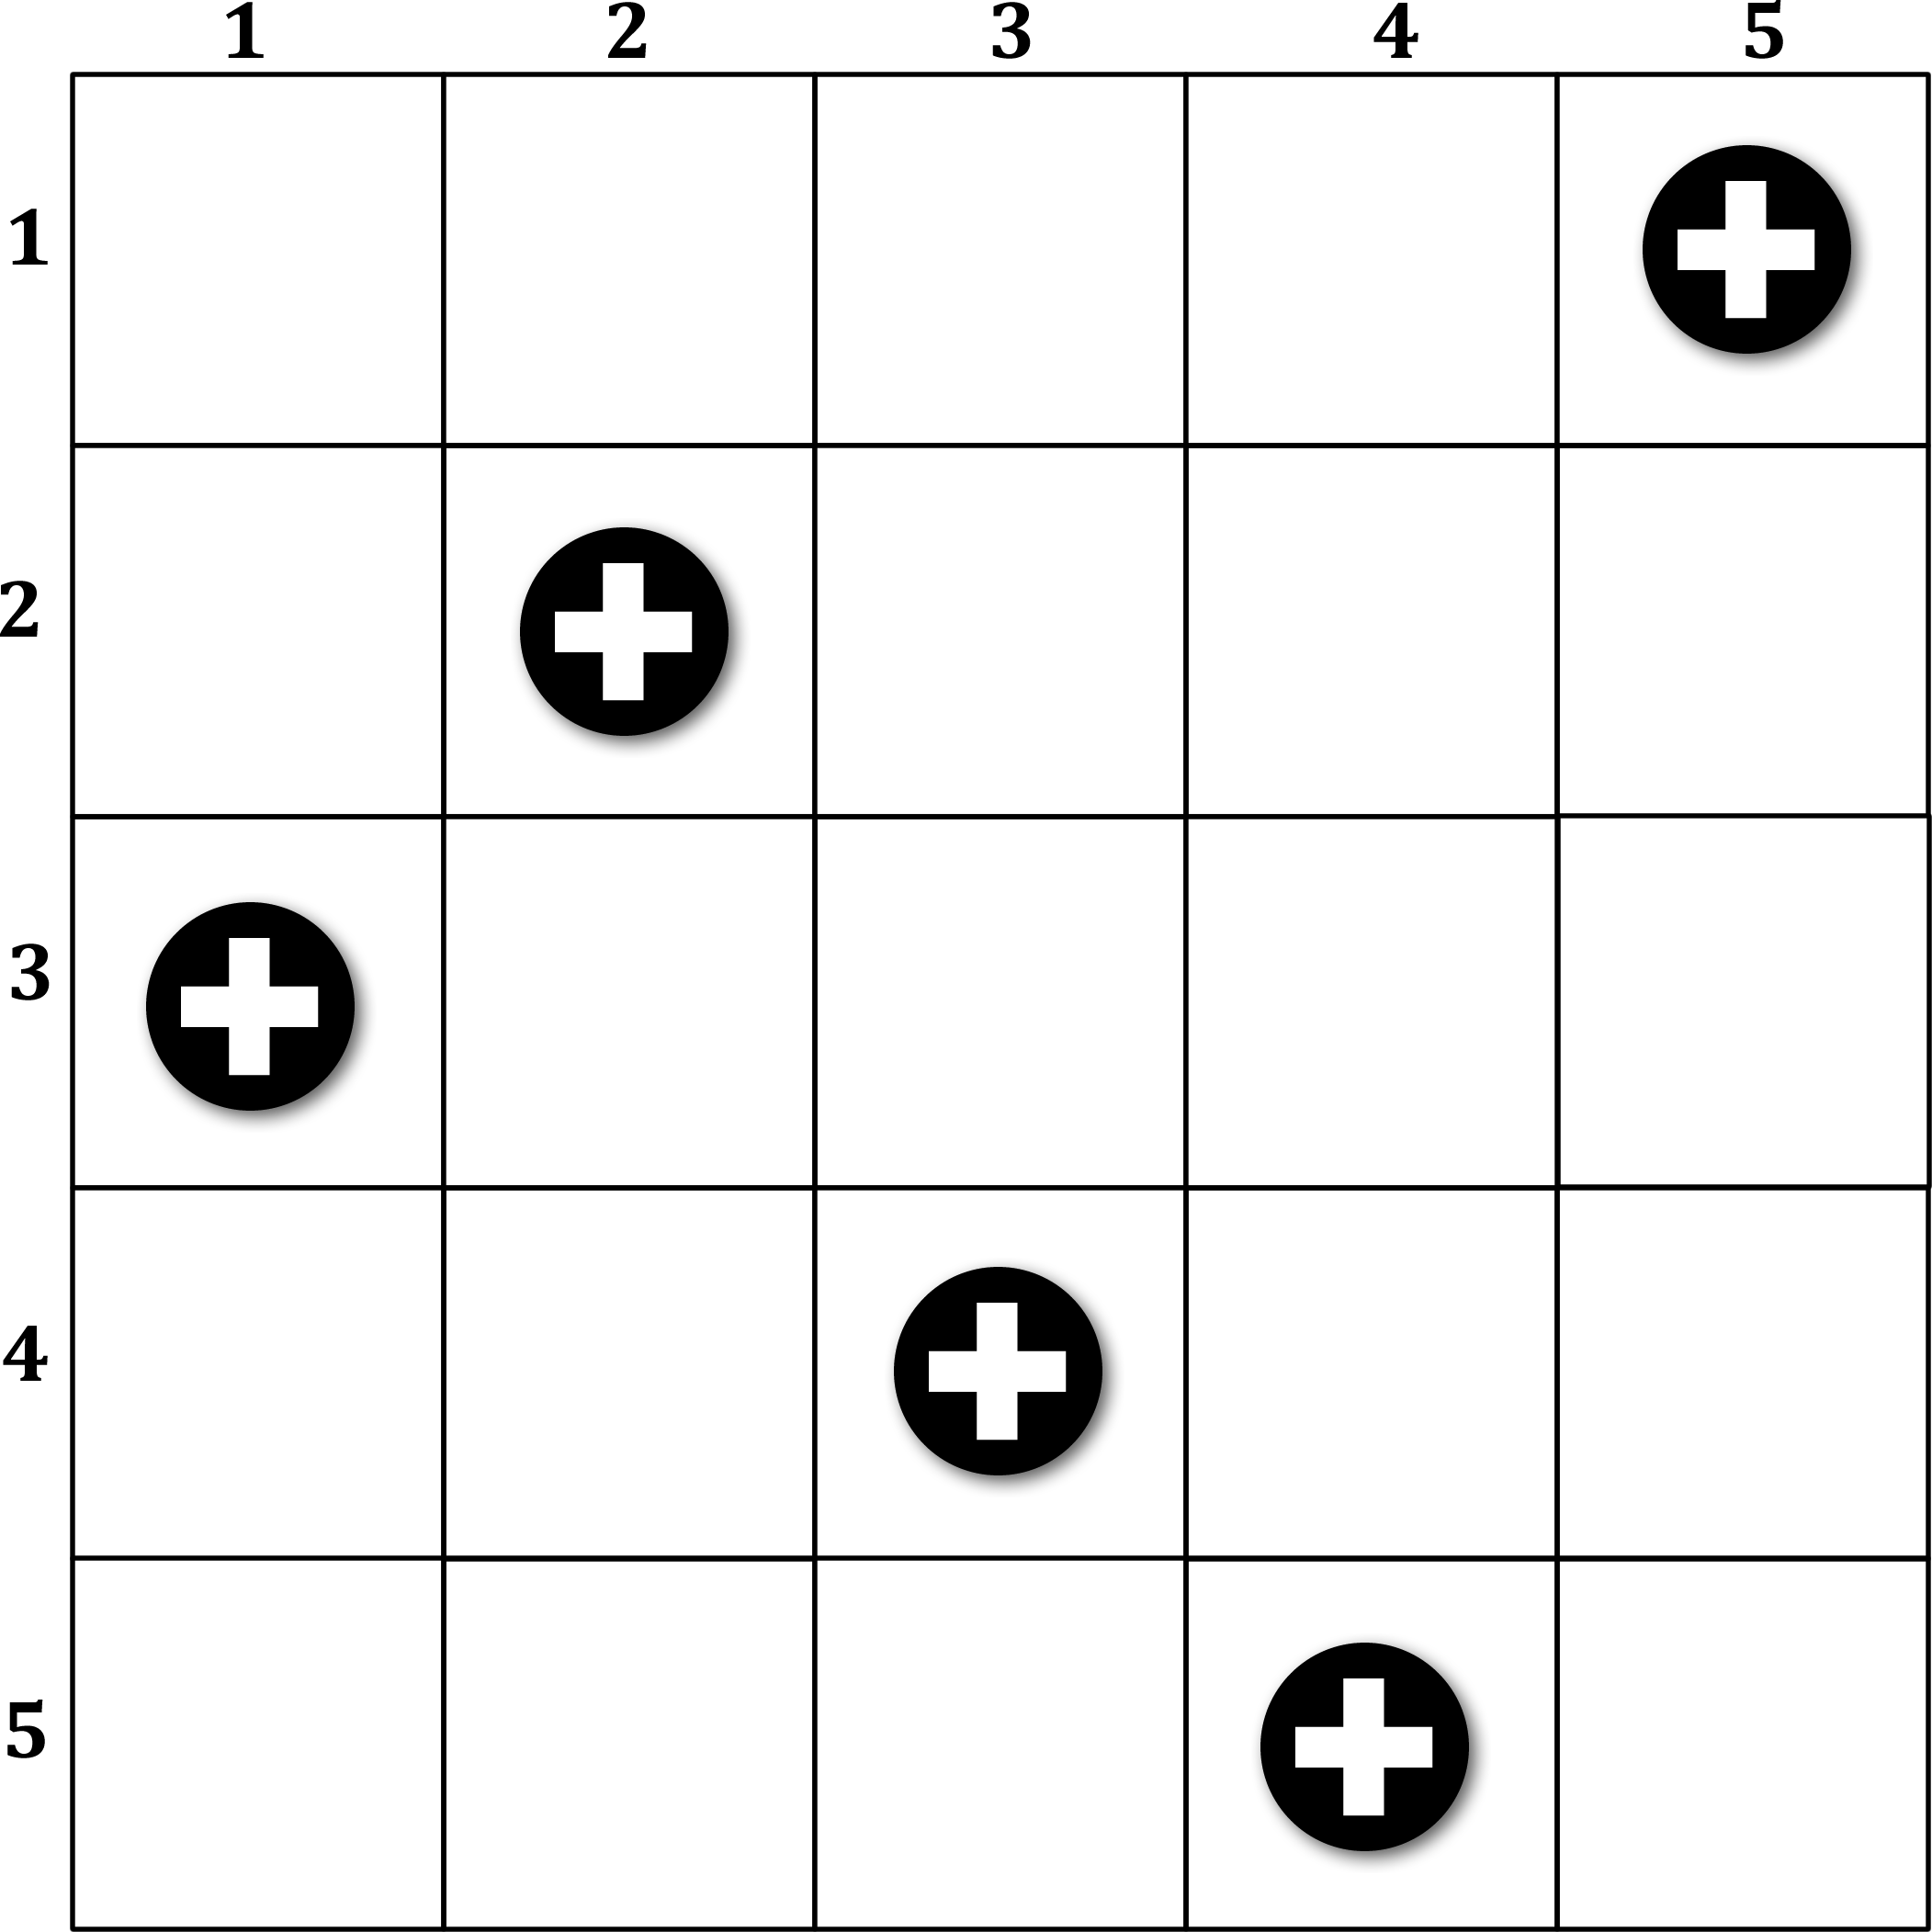
\includegraphics[width=0.35\linewidth]{costas.png}
\caption[]{Example of marks for \CARRP}
\label{fig:ex_costas}
\end{figure}

\new{The cost of the configuration $s$ is then the number of equal elements on each row $d_i$ of its corresponding differences triangle. It can be easily proved that this differences triangle is only necessary to be verified until the row $d_B$, with $B=\floor*{(n-1)/2}$.}

\subsection{Experiments design and results}

To handle this problem, I have reused all modules used for solving the \nqp. First attempts to solve this problems were using the same strategies (\ass) used to solve the \sgp{} and \nqp, without success: \posl{} was not able to solve instances larger than $n = 8$ in a reasonable amount of time (seconds). After many unsuccessful attempts to find the right parameters of \textit{maximum number of restarts}, \textit{maximum number of iterations}, and \textit{maximum number of iterations with the same cost}, I decided to implement the mechanism used by Daniel D\'iaz in the current implementation of {\it Adaptive Search} to escape from local minima: I have added a {\it Reset} \om{} $R_{AS}$ based on the abstract \om{} $R$. The other \oms{} were the same used for solving the \nqp.

Given a configuration $s$, the basic principle of the reset is build another following four steps:
\begin{enumerate}
\item A configuration is obtained by performing left/right shifts to all sub-vectors of $s$ starting or ending by the variable which contributes the most to the cost, and selecting the configuration with the lowest cost.
\item A configurations is obtained by adding a constant (circularly) to each element in the configuration $s$.
\item A configuration is obtained by shifting left from the beginning of $s$ to some culprit variable (i.e. a variable contributing to the cost).
\item Then, one of these 3 generated configuration has the same probability of being selected, to be the result of the reset algorithm. In that sense, some different resets can be performed for the same configuration.
\end{enumerate}


The basic solver used to solve this problem is presented in Algorithm~\ref{as:costas}, and it was taken as a base to build all the different communication strategies. Basically, it is a classical local search iteration, where instead of performing restarts, it performs resets. After a deep analysis of this implementation and results of some runs, I decided to use $K_1 = 2,000,000$ (maximum number of iterations) big enough to solve the chosen instance $n = 19$; and $K_2 = 3$ (the number of iteration before performing the next \textit{reset}).

\begin{algorithm}[H]
\dontprintsemicolon
\SetNoline
\SetKwProg{myproc}{\tet{\bf abstract solver}}{\tet{\bf begin}}{\tet{\bf end}}
\myproc{as\_hard \tcp*{{\sc Itr} $\rightarrow$ number of iterations}
	\tet{\bf computation} : $I, R, V, S, A$\;}{ %\tcp*{{\sc Sci} $\rightarrow$ number of iterations with the same cost}}{%
	$I \poslop{\mapsto}$
	\whileinline{$\left(\textbf{\Iter < } K_1\right)$}{
		$R \poslop{\mapsto}$ % \left[\circlearrowleft (\text{\Iter}\% K_2) \left\{ M_V \longmapsto M_{\hat{S}} \longmapsto M_D\right\}\right]$\;
		\whileinline{$\left(\textbf{\Iter \% } K_2\right)$}{$\left[V \poslop{\mapsto} S \poslop{\mapsto} A\right]$}
	}
}
\tet{\bf solver} \solverposl{single} \tet{\bf implements} as\_hard\;
\algoindent \tet{\bf computation} : $I_{perm},  R_{AS}, V_{AS}, S_{first}, A_{AI}$ \;
%\tet{\bf connection}: $CM_{last}$\;
\caption{Reset-based \as{} for \CARRP}\label{as:costas}
\end{algorithm}

Table~\ref{tab:costas19} shows results of launching \sosets{} to solve each instance of \carrp{} 19 sequentially and in parallel without communication. Runtimes and iteration means showed in this confirm once again the success of the parallel approach. 

\begin{table}[h]
\captionsetup{belowskip=6pt,aboveskip=6pt}
\centering
\renewcommand{\arraystretch}{1}
\begin{tabular}{p{3.5cm}|R{1.5cm}R{1cm}R{1.7cm}R{1.7cm}R{2cm}}
	\hline
	{\bf STRATEGY} & T & T(ds) & It. & It.(sd) & \% success\\
	\hline
	%\hline
	Sequential (1 core) & 132.73 & 80.32 & 2,332,088 & 1,424,757 & 40.00\\
	Parallel (40 cores) & 25.51 & 15.75 & 231,262 & 143,789 & 100.00\\
	\hline
\end{tabular}
\caption{\carr{} 19: no communication}
\label{tab:costas19}
\end{table}

\separation

In order to improve results, a simple communication strategy was applied: communicating the current configuration to other solvers. To do so, we insert a \textit{sending output} operator to the \as{} in Algorithm~\ref{as:costas}. This results in the sender solver presented in Algorithm~\ref{as:costas_sender}. %\tet{et le receiver??? Flo: c'est l'algo 4}

\begin{algorithm}[h]
\dontprintsemicolon
\SetNoline
\SetKwProg{myproc}{\tet{\bf abstract solver}}{\tet{\bf begin}}{\tet{\bf end}}
\myproc{as\_hard\_sender \; %\hspace{3pt}
	\tet{\bf computation} : $I, R, V, S, A$\;}{
	$I \poslop{\mapsto}$
	\whileinline{$\left(\textbf{\Iter} < K_1\right)$}{
		$T \poslop{\mapsto}$
		\whileinline{$\left(\textbf{\Iter \% } K_2\right)$}{$\left[V \poslop{\mapsto} S \poslop{\mapsto} \llparenthesis A \rrparenthesis^d\right]$}
	}
}
\tet{\bf solver} \solverposl{sender} \tet{\bf implements} as\_hard\_sender\;
\algoindent \tet{\bf computation} : $I_{perm}, R_{AS}, V_{AS}, S_{first}, A_{AI}$ \;
%\tet{\bf connection}: $CM_{last}$\;
\caption{Sender solver for \CARRP}\label{as:costas_sender}
\end{algorithm}

Studying some runs of \posl{} solving \CARRP{}, it was observed that \new{during the search process, the cost of the current configuration of all solvers describes an oscillatory descent due to the repeated resets ($K_2 = 3$ in Algorithm~\ref{as:costas}). It means that the cost of the current configuration decreases during $K_2$ iterations and then the current configuration is created by performing a reset which generates generally a more costly configuration. However, in every performed experiment (more than 20 runs with 20 solvers in parallel without communication), the current configuration's cost of the winner solver (first solver finding a solution) described an oscillatory descent also, but not so pronounced (i.e. the difference between the cost of the last current configuration before performing the reset and the cost of the configuration after the reset is not high).} For that reason, it was decided to apply a simple \commstr{} that shares the current configuration while applying the acceptance criterion. To do so, a \opch{} using a \textit{minimum} operator $\poslop{m}$ together with the abstract \om{} $A$ was inserted, as shown in Algorithm~\ref{as:costas_receiver_a}.

One of the main purpose of this study is to explore different communication strategies. We have then implemented and tested different variations of the strategy exposed above by combining two communication operators (\oneTone{} and \oneTn) and different percentages of communicating solvers.
For this problem, it was study also the behavior of the communication performed at two different moments: while applying the acceptance criteria (Algorithm~\ref{as:costas_receiver_a}), and while performing a {\it reset} (Algorithm~\ref{as:costas_receiver_b}).

\begin{algorithm}[h]
\dontprintsemicolon
\SetNoline
\SetKwProg{myproc}{\tet{\bf abstract solver}}{\tet{\bf begin}}{\tet{\bf end}}
\myproc{as\_hard\_receiver\_a \tcp*{{\sc Itr} $\rightarrow$ number of iterations}
	\tet{\bf computation} : $I, T, V, S, A$ \; %\hspace{3pt}
	\tet{\bf communication} : $C.M.$\;}{ 
	$I \poslop{\mapsto}$
	\whileinline{$\left(\textbf{\Iter} < K_1\right)$}{
		$T \poslop{\mapsto}$
		\whileinline{$\left(\textbf{\Iter \% } K_2\right)$}{$\left[V \poslop{\mapsto} S \poslop{\mapsto} \left[A\poslop{m}C.M.\right]\right]$}
	}
}
\tet{\bf solver} \solverposl{receiverA} \tet{\bf implements} as\_hard\_receiver\_a\;
\algoindent\tet{\bf computation} : $I_{perm}, R_{AS}, V_{AS}, S_{first}, A_{AI}$ \; 
\algoindent\tet{\bf communication}: $CM_{last}$\;
\caption{Receiver solver for \CARRP{} (variant A)}\label{as:costas_receiver_a}
\end{algorithm}

\begin{algorithm}[h]
\dontprintsemicolon
\SetNoline
\SetKwProg{myproc}{\tet{\bf abstract solver}}{\tet{\bf begin}}{\tet{\bf end}}
\myproc{as\_hard\_receiver\_b \tcp*{{\sc Itr} $\rightarrow$ number of iterations}
	\tet{\bf computation} : $I, R, V, S, A$\; %\tcp*{{\sc Sci} $\rightarrow$ number of iterations with the same cost}
	\tet{\bf communication} : $C.M.$\;}{%
	$I \poslop{\mapsto}$
	\whileinline{$\left(\textbf{\Iter < } K_1\right)$}{
		$\left[R \poslop{m} C.M.\right] \poslop{\mapsto}$
		\whileinline{$\left(\textbf{\Iter \% } K_2\right)$}{$\left[V \poslop{\mapsto} S \poslop{\mapsto} A\right]$}
	}
}
\tet{\bf solver} \solverposl{receiverB} \tet{\bf implements} as\_hard\_receiver\_b\;
\algoindent\tet{\bf computation} : $I_{perm}, R_{AS}, V_{AS}, S_{first}, A_{AI}$ \; 
\algoindent\tet{\bf connection}: $CM_{last}$\;
\caption{Receiver solver for \CARRP{} (variant B)}\label{as:costas_receiver_b}
\end{algorithm}

The instantiation for receiver solvers instantiates the abstract \opch{} $C.M.$ with the concrete \opch{} $CM_{last}$, which takes into account the last received configuration at the time of its execution.

\begin{table}
\centering 
\renewcommand{\arraystretch}{1}
\resizebox{\columnwidth}{!}{%
\begin{tabular}{p{2.5cm}|R{1.1cm}R{1cm}R{1.3cm}R{1.3cm}|R{1cm}R{1cm}R{1.3cm}R{1.3cm}}
	\hline
	\multirow{3}{*}{\footnotesize{\centering {\bf STRATEGY}}} & \multicolumn{4}{c}{100\% COMM} & \multicolumn{4}{c}{50\% COMM} \\
	\cline{2-9}
	& T & T(sd) & It. & It.(sd) & T & T(sd) & It. & It.(sd)\\
	\hline
	Str A: 1 to 1 & 11.60 & 9.17 & 84,159 & 68,958 & 16.78 & 13.43 & 148,222 & 121,688 \\
	Str A: 1 to N & \good{10.83} & 8.72 & 79,551 & 63,785 & 13.03 & 13.46 & 106,826 & 120,894 \\	
	Str B: 1 to 1 & 14.84 & 13.54 & 119,635 & 112,085 & 14.51 & 13.88 & 125,982 & 123,261 \\
	Str B: 1 to N & 22.99 & 23.82 & 199,930 & 207,851 & 16.62 & 15.16 & 138,840 & 116,858 \\
	\hline
\end{tabular}
}
\caption{\carr{} 19: with communication}
\label{tab:costas19comm}
\end{table}

Table~\ref{tab:costas19comm} shows that \sosets{} executing the strategy {\it A} (receiving the configuration at the time of applying the acceptance criteria) are more effective. \new{The main reason is because in the \commstr{} {\it B}, the communication interferes with the proper performance of the {\it reset}, which is a very important step in the algorithm. Furthermore, the reset provides a very important exploratory factor: when receivers solvers receive the sent configurations and it is accepted by them, they can performed different resets with the same configuration, as it was explained before.}
 
By analyzing the whole information obtained during the experiments, we can observe that the percentage of communicating solvers finding the solution thanks to the received information was high (74\%, see Appendix~\ref{app:cap}, Figure~\ref{barplot:19}). That shows that the communicated information was very helpful during the search process. 
With the simplicity of the operator-based language provided by \posl{}, we were able to find a simple \commstr{} to obtain better results than applying sequential and parallel independent multi-walk approaches. 

\new{Algorithm~\ref{comm:costas1001N} shows the code for the \commstr{} of 100\% of communicating solvers using the \oneTn{} operator $\oneton$. %, where  20 is used as  \textit{syntactic sugar} to declare easily a list of 20 solvers of each type (20 senders and 20 receivers). 
As expected, this was the best \commstr{}. It finds a proper equilibrium between intensification, by communicating a promising place (configuration) inside the search space to a maximum of solvers; and exploration, by performing stochastic decisions once the configuration is accepted, e.g. the must culprit variable is randomly selected if there are more than one, and the way the reset select the returned configuration (explained before).}
%(a good compromise between local computation and data exchange/a fully based communication/ etc) 

\begin{algorithm}
\dontprintsemicolon
\SetNoline
$\left[\eqsolverposl{sender}\posldot A(20)\right] \oneton \left[\eqsolverposl{receiverA}\posldot C.M.(20)\right];$
\caption{Communication strategy \oneTn{} 100\% for \CARRP}\label{comm:costas1001N}
\end{algorithm}

\new{The random nature of this solution strategy has showed to be effective. However, it is the explanation to the high values of standard deviation showe in Table~\ref{tab:costas19comm}. \Ass{} used to the resolution of \CARRP{} combine \oms{} which take many stochastic decisions. The neighborhood \om{} compute the neighborhood based on the most culprit variable of the input configuration, which is randomly selected if there exist more than one. This \m{} also generates neighbors by selecting randomly the variables to swap. In addiction, the reset \om{} generates configurations in three different ways and equally probable, for a same input configuration.}

%\begin{algorithm}[H]
%\dontprintsemicolon
%\SetNoline
%\SetKwProg{myproc}{\tet{\bf abstract solver}}{\tet{\bf begin}}{\tet{\bf end}}
%\myproc{as\_hard\_receiver\_a \tcp*{{\sc Itr} $\rightarrow$ number of iterations}
%	\tet{\bf computation} : $I, R, V, S, A$\; %\tcp*{{\sc Sci} $\rightarrow$ number of iterations with the same cost}
%	\tet{\bf communication} : $C.M.$\;}{%
%	$I \poslop{\mapsto}$\\
%	\While{$\left(\textbf{\Iter < } K_1\right)$}{
%		$R \poslop{\mapsto}$
%		\whileinline{$\left(\textbf{\Iter \% } K_2\right)$}{$\left[V \poslop{\mapsto} S \poslop{\mapsto} \left[A \poslop{m} C.M.\right]\right]$}
%	}
%}
%\caption{Reset-based \as{} for \CARRP{} (receiver, variant A)}\label{as:costas_receiver_a}
%\end{algorithm}
%
%
%\begin{algorithm}[H]
%\dontprintsemicolon
%\SetNoline
%\SetKwProg{myproc}{\tet{\bf abstract solver}}{\tet{\bf begin}}{\tet{\bf end}}
%\myproc{as\_hard\_receiver\_c \tcp*{{\sc Itr} $\rightarrow$ number of iterations}
%	\tet{\bf computation} : $I, R, V, S, A$\; %\tcp*{{\sc Sci} $\rightarrow$ number of iterations with the same cost}
%	\tet{\bf communication} : $C.M.$\;}{%
%	$I \poslop{\mapsto}$\\
%	\While{$\left(\textbf{\Iter < } K_1\right)$}{
%		$\left[R \poslop{m} C.M.\right] \poslop{\mapsto}$
%		\whileinline{$\left(\textbf{\Iter \% } K_2\right)$}{$\left[V \poslop{\mapsto} S \poslop{\mapsto} A\right]$}
%	}
%}
%\caption{Reset-based \as{} for \CARRP{} (receiver, variant C)}\label{as:costas_receiver_c}
%\end{algorithm}

\section{Solving the \grp}
\label{sec:golomb}

\modified{In this section I present the performed study using \grp{} (\GRP) as a benchmark.}

\subsection{Problem definition}

\modified{The \grp{} (\GRP) problem consists in finding an ordered vector of $n$ distinct non-negative integers, called \textit{marks}, $m_1 < \dots < m_n$, such that all differences $m_i - m_j$ $(i > j)$ are all different. An instance of this problem is the pair $(o,l)$ where $o$ is the order of the problem, (i.e., the number of \textit{marks}) and $l$ is the length of the ruler (i.e., the last {\it mark}). We assume that the first \textit{mark} is always 0. This problem has been applied to radio astronomy, x-ray crystallography, circuit layout and geographical mapping \cite{Soliday1995}. 
When I apply \posl{} to solve an instance of this problem sequentially, I can notice that it performs many {\it restarts} before finding a solution. For that reason I have chosen this problem to study a new communication strategy.}

\modified{The cost function is implemented based on the storage of a counter for each measure present in the rule (configuration). I also store all distances where a variable is participating. This information is usefull to compute the more culprit variable (the variable that interfiers less in the representd measures), in case of the user wants to apply algorithms like {\it Adaptive Search}. This cost is calculated in $O\left(o^2 + l\right)$.}

\subsection{Experiment design}

\modified{I use \grp{} instances to study a different communication strategy. This time I communicate the current configuration, to avoid its neighborhood, i.e., a {\it tabu} configuration. I have reused some modules used in the resolution of \sg{} and \carr{} problems to design the solvers: the \textit{Selection} and \textit{Acceptance} modules. The new modules are:}

\begin{enumerate}
	\item Generation module:
	\subitem \modified{$I$: Generates a random configuration $s$, respecting the structure of the problem, i.e., the configuration is an ordered vector of integers. This module takes into account a set of {\it tabu} configurations arrived from the same solver, and also via solver-communication through a \opch{} $C.M.$ that receives a set of configurations. This module constructs the new configuration far enough from the {\it tabu} configurations.}
	\item Neighborhood module:
	\subitem \modified{$V$: Defines the neighborhood $\mathcal{V}\left(s\right)$ by changing one value while keeping the order, i.e., replacing the value $s_i$ by all possible values $s'_i \in D_i$ that satisfy $s_{i-1} < s'_i < s_{i+1}$.}
\end{enumerate}

\modified{I also add a module to insert a configuration into a \textit{tabu} list inside the solver. In Algorithm~\ref{as:golomb_sender} the \as{} used to send information (sender \as) is presented. When the module $T$ is executed, the solver is unable to find a better configuration around the current one, so it is assumed to be a local minimum, and it is sent to the receiver solver. Algorithm~\ref{as:golomb_receiver} presents an \as{} used to receive information (receiver \as). Based on the connection operator used in the communication strategy, this solver might receives one or many configurations. These configurations are the input of the generation module ($I$), and this module inserts all received configurations into a {\it tabu} list, and then generates a new first configuration, far from all configurations in the {\it tabu} list.}

\begin{algorithm}
\dontprintsemicolon
\SetNoline
\SetKwProg{myproc}{\tet{\bf abstract solver}}{\tet{\bf begin}}{\tet{\bf end}}
\myproc{as\_golomb\_sender \tcp*{{\sc Itr} $\rightarrow$ number of iterations}
	\tet{\bf computation} : $I, V, S, A, T$\;}{
	\While{$\left(\textbf{\Iter < } K_1\right)$}{
		$I \poslop{\mapsto}$ 
		\whileinline{$\left(\textbf{\Iter \% } K_2\right)$}{$\left[V \poslop{\mapsto} S \poslop{\mapsto} A\right]$} $\poslop{\mapsto} \llparenthesis T \rrparenthesis^o$
	}
}
\caption{\As{} for \GRP{} (sender)}\label{as:golomb_sender}
\end{algorithm}

\begin{algorithm}
\dontprintsemicolon
\SetNoline
\SetKwProg{myproc}{\tet{\bf abstract solver}}{\tet{\bf begin}}{\tet{\bf end}}
\myproc{as\_golomb\_receiver \tcp*{{\sc Itr} $\rightarrow$ number of iterations}
	\tet{\bf computation} : $I, V, S, A, T$\;
	\tet{\bf connection} : $C.M.$\;}{
	\While{$\left(\textbf{\Iter < } K_1\right)$}{
		$\left[C.M. \poslop{\mapsto} I \right] \poslop{\mapsto}$ 
		\whileinline{$\left(\textbf{\Iter \% } K_2\right)$}{$\left[V \poslop{\mapsto} S \poslop{\mapsto} A\right]$} $\poslop{\mapsto} \llparenthesis T \rrparenthesis^o$
	}
}
\caption{\As{} for \GRP{} (receiver)}\label{as:golomb_receiver}
\end{algorithm}

\modified{In this communcation strategy there are some parameters to be tuned. The first ones are:} \begin{inparaenum}[1.] \item $K_1$, the number of restarts, and \item $K_2$, the number of iterations by restart. \end{inparaenum} Both are instance dependent, so, after many experimental runs, I choose them as follows:
\begin{itemize}
\item \gr{} 8--34: $K_1 = 300$ and $K_2 = 200$
\item \gr{} 10--55: $K_1 = 1000$ and $K_2 = 1500$
\item \gr{} 11-72: $K_1 = 1000$ and $K_2 = 3000$
\end{itemize}

\modified{The other parameters are related to the behavior of the {\it tabu list}:}

\modified{The idea of this strategy (\as) follows the following steps:}

\poslexample{
\mybox{Step 1}

The \om{} generates an initial configuration tacking into account a set of configurations into a {\it tabu list}. The configuration arriving to this {\it tabu list} come from the same solver (Step 3) or from outside (other solvers) depending on the strategy (non-communicating or communicating).

This module applies some other modules provided by \posl{} to solve the {\it Sub-Sum Problem} in order to generates {\it valid} configurations for \grp{}. A valid configuration $s$ for \grp{} is a configuration that fulfills the following constraints:

\begin{itemize}
\item $s = \left(a_1, \dots, a_o\right)$ where $a_i < a_j, \forall i < j$, and
\item all $d_i = a_{i+1} - a_i$ are all different, for all $d_i, i\in[1...o-1]$
\end{itemize}

The {\it Sub-sum Problem} is defined as follows: Given a set $E$ of integers, with $\left|E\right| = N$, finding a sub set $e$ of $n$ elements that sums exactly $z$. In that sense, a solution $S_{sub-sum} = \left\{s_1, \dots, s_{o-1}\right\}$ of the {\it Sub-sum problem} with $E = \left\{1, \dots, l-\tfrac{(o-2)(o-1)}{2}\right\}$, $n = o-1$ and $z = l$, can be traduced to a {\it valid} configuration $C_{grp}$ for \grp{} as follows:
$$C_{grp} = \left\{c_1, c_1+s_1, \dots, c_{o-1}+s_{o-1}\right\}$$
where $c_1 = 0$.

In the selection module applied inside the module $I$, the selection step of the search process selects a configuration from the neighborhood {\it far} from the {\it tabu} configurations, with respect to certain vectorial norm and an epsilon. In other words, a configuration $C$ is selected if and only if:
\begin{enumerate}
\item the cost of the configuration $C$ is lower than the current cost, and
\item $\left|\left|C-C_t\right|\right|_p > \epsilon$, for all {\it tabu} configuration $C_t$
\end{enumerate}
where $p$ and $\epsilon$ are parameters.

I experimented with 3 different values for $p$. Each value defines a different type of norm of a vector $x = \left\{x_1, \dots, x_n\right\}$:
\begin{itemize}
\item $p = 1$:  $\left|\left|x\right|\right|_1 = \sum_{i=0}^{n}{\left|x_i\right|}$
\item $p = 2$:  $\left|\left|x\right|\right|_2 = \sqrt{\sum_{i=0}^{n}{\left|x_i\right|^2}}$
\item $p = \infty$:  $\left|\left|x\right|\right|_{\infty} = \max{(x)}$
\end{itemize}

After many experimental runs with these values I choose $p = \infty$ and $\epsilon = 4$ for the communication strategy study. I also made experiments trying to find the right size for the {\it tabu} list and the conclusion was that the right sizes were $15$ for non-communicating strategies and $40$ for communicating strategies, taking into account that in the latter, I work with 20 receivers solvers.
}

\poslexample{
\mybox{Step 2}

After generating the first configuration, the next step is to apply a local search to improve it. In this step I use the neighborhood \om{} $V$, that creates neighborhood $\mathcal{V}\left(s\right)$ by changing one value while keeping the order in the configuration, and the other modules (selection and acceptance). The local search is executed a number $K_2$ of times, or until a solution is obtained.
}

\poslexample{
\mybox{Step 3}

If no improvement is reached, the current configuration is classified as a {\it potential local minimum} and inserted into the {\it tabu} list. Then, the process returns to the Step 1. 
}

\subsection{Analysis of results}

\modified{The benefit of the parallel approach is also proved for the \grp{} (see Table~\ref{tab:golomb_sec} with respect to \ref{tab:golomb_par_notabu}, \ref{tab:golomb_par_tabu}, \ref{tab:golomb_par_1-1} and \ref{tab:golomb_par_1-n}). But the main goal of choosing this benchmark was to study a different communication strategy, since for solving this problem, \posl{} needs to perform some restarts. In this communication strategy, solvers do not communicate the current configuration to have more solvers searching in its neighborhood, but a configuration that we assume is a local minimum to be avoided. We consider that the current configuration is a local minimum since the solver (after a given number of iteration) is not able to find a better configuration in its neighborhood, so it will communicate this configuration just before performing the restart.}

\modified{The first experiment compares the runs of non communitaing solvers not using a {\it tabu} list with non communicating solvers using a {\it tabu} list. The results in Tables~\ref{tab:golomb_par_notabu} and \ref{tab:golomb_par_tabu} demonstrate that using a {\it tabu} list can help the search process. Without communication, the improvement is not substantial (8\% for 8--34, 7\% for 10--55 and 5\% for 11--72). The reason is because only one configuration is inserted in the \textit{tabu} list after each restart. When we use \textit{1~to~1} communication, after the restart $k$, the receiving solver has twice the number of configurations in the \textit{tabu} list (one {\it tabu} configuration from itself and the received one after each restart). Table~\ref{tab:golomb_par_1-1} shows that this strategy is not sufficient for some instances, but when we use \textit{1~to~N} communication, the number of \textit{tabu} configurations after the restart $k$, in the receiving solver is considerably higher, e.g., after the restart $k$ a receiving solver has $k(N+1)$ configurations in his \textit{tabu} list (one {\it tabu} configuration from itself and $N$ received from the other solvers, each restart). Hence, these solvers can generate configurations far enough from many potentially local minima. This phenomenon is more visible when the problem order increases. Table~\ref{tab:golomb_par_1-n} shows that the improvement for the higher case (11-72) is about 32\% with respect to non communicating solvers without using a {\it tabu} list (Table~\ref{tab:golomb_par_notabu}), and about 29\% with respect to non communicating solvers using a {\it tabu} list (Table~\ref{tab:golomb_par_tabu}).}

\vspace{18pt}

\begin{table}[h]
	%\captionsetup{belowskip=6pt,aboveskip=6pt}
	\centering 
	\renewcommand{\arraystretch}{1}
		\begin{tabular}{p{2cm}|R{1.2cm}R{1.2cm}|R{1.5cm}R{1.5cm}|R{0.8cm}R{1.2cm}|R{2cm}}
			\hline 	
			{\bf Instance} & T & T(sd) & It. & It.(sd) & R & R(sd) & \% success\\
			\hline
			8--34 & 0.79 & 0.66 & 13,306 & 11,154 & 66 & 55.74 & 100.00\\
			8--34 (t) & 0.66 & 0.63 & 10,745 & 10,259 & 53 & 51.35 & 100.00 \\
			10--55 & 66.44 & 49.56 & 451,419 & 336,858 & 301 & 224.56 & 80.00\\			
			10--55 (t) & 67.89 & 50.02 & 446,913 & 328,912 & 297 & 219.30 & 88.00\\
			11--72 & 160.34 & 96.11 & 431,623 & 272,910 & 143 & 90.91 & 26.67\\
			11--72 (t) & 117.49 & 85.62 & 382,617 & 275,747 & 127 & 91.85 & 30.00\\
			\hline
		\end{tabular}
	\caption{\gr: a single sequential solver}
	\label{tab:golomb_sec}
\end{table}

\begin{table}[h]
	%\captionsetup{belowskip=6pt,aboveskip=6pt}
	\centering 
	\renewcommand{\arraystretch}{1}
	\begin{tabular}{p{2cm}|R{1.2cm}R{1.2cm}|R{1.5cm}R{1.5cm}|R{0.8cm}R{1.2cm}}
		\hline 	
		{\bf Instance} & T & T(sd) & It. & It.(sd) & R & R(sd)\\
		\hline
		%\hline
		8--34 & 0.47 & 34.82 & 436 & 330.10 & 2 & 1.63\\
		10--55 & 5.31 & 38.63 & 22,577 & 16,488 & 15 & 11.00\\
		11--72 & 89.76 & 55.85 & 164,763 & 102,931 & 54 & 34.32\\
		\hline
	\end{tabular}
	\caption{\gr: parallel, without tabu list.}
	\label{tab:golomb_par_notabu}
\end{table}

\begin{table}[h]
	%\captionsetup{belowskip=6pt,aboveskip=6pt}
	\centering 
	\renewcommand{\arraystretch}{1}
	\begin{tabular}{p{2cm}|R{1.2cm}R{1.2cm}|R{1.5cm}R{1.5cm}|R{0.8cm}R{1.2cm}}
		\hline 	
		{\bf Instance} & T & T(sd) & It. & It.(sd) & R & R(sd)\\
		\hline
		%\hline
		8--34 & 0.43 & 0.37 & 349 & 334 & 1 & 1.64\\
		10--55 & 4.92 & 4.68 & 20,504 & 19,742 & 13 & 13.07\\
		11--72 & 85.02 & 67.22 & 155,251 & 121,928 & 51 & 40.64\\
		\hline
	\end{tabular}
	\caption{\gr: parallel, with tabu list.}
	\label{tab:golomb_par_tabu}
\end{table}

\begin{table}[h]
	%\captionsetup{belowskip=6pt,aboveskip=6pt}
	\centering 
	\renewcommand{\arraystretch}{1}
	\begin{tabular}{p{2cm}|R{1.2cm}R{1.2cm}|R{1.5cm}R{1.5cm}|R{0.8cm}R{1.2cm}}
		\hline 	
		{\bf Instance} & T & T(sd) & It. & It.(sd) & R & R(sd)\\
		\hline
		%\hline
		8--34 & 0.44 & 0.31 & 309 & 233 & 1 & 1.23\\
		10--55 & 3.90 & 3.22 & 15,437 & 12,788 & 10 & 8.52\\
		11--72 & 85.43 & 52.60 & 156,211 & 97,329 & 52 & 32.43\\
		\hline
	\end{tabular}
	\caption{\gr: parallel, communication 1 to 1.}
	\label{tab:golomb_par_1-1}
\end{table}

\begin{table}[h]
	%\captionsetup{belowskip=6pt,aboveskip=6pt}
	\centering 
	\renewcommand{\arraystretch}{1}
	\begin{tabular}{p{2cm}|R{1.2cm}R{1.2cm}|R{1.5cm}R{1.5cm}|R{0.8cm}R{1.2cm}}
		\hline 	
		{\bf Instance} & T & T(sd) & It. & It.(sd) & R & R(sd)\\
		\hline
		%\hline
		8--34 & 0.43 & 0.29 & 283 & 225 & 1 & 1.03\\
		10--55 & 3.16 & 2.82 & 12,605 & 11,405 & 8 & 7.61\\
		11--72 & 60.35 & 43.95 & 110,311 & 81,295 & 36 & 27.06\\
		\hline
	\end{tabular}
	\caption{\gr: parallel, communication 1 to n.}
	\label{tab:golomb_par_1-n}
\end{table}

\section{Summarizing}

\modified{In this Chapter} I have chosen various \CSPs{} as benchmarks to \begin{inparaenum}[1.] \item evaluate the \posl{} behavior solving these kind of problems, and \item to study different solution strategies, specially communication strategies.\end{inparaenum} To this end, I have chosen benchmarks with different characteristics, to help me having a wide view of the \posl{} behavior.

\modified{In the solution process} of \sgp{}, it was showed the success of an exploitation-oriented communication strategy, in which the current configuration is communicated to ask other solvers for help, concentrating the effort in a more promising area. I was able also to study some other unsuccessful strategies, to show that strategies based on the sub-division of the effort by weeks, is not a good idea.

\modified{It was showed that simple communication strategies} as they applied to solve \sgp{} does not improve enough the results without communication for the \nqp{}. However, a deep study of the \posl's behavior during the search process allows to design a communication strategy able to improve the results obtained using non-communicating strategies.

\modified{The \carrp{} is a very complicated constrained problem, and very sensitive to the methods to solve it. For that reason I used some ideas from already existent algorithms. However, thanks to some studies of different communication strategies, based on the configuration of the current communication at different times (places) in the algorithm, it was possible to find a communication strategy to improve the performance.}

\modified{During the solution} process of the \grp{}, \posl{} needs to perform many restarts. For that reason, this problem was chosen to study a different (and innovative up tu my knowledge) communication strategy, in which the communicated information is a potential local minimum to be avoided. This new communication strategy showed to be effective to solve these kind of problems.

\modified{In all cases,} thanks to the operator-based language provided by \posl{} it was possible to test many different strategies (communicating and non-communicating) fast and easily. Whereas creating solvers implementing different solution strategies can be complex and tedious, \posl{} gives the possibility to make communicating and non-communicating solver prototypes and to evaluate them with few efforts. In this Chapter it was possible to show that a good selection and management of inter-solvers communication can largely help to the search process, working with complex constrained problems.

%%%----------------------------------------------------------------------------------------------
%------ RESULTS
%----------------------------------------------------------------------------------------------
\chapter{Analysis of results}
\label{chap:res}
\textit{In this chapter we explain the used environments were we run the experiments (description of my desktop machine, \textit{Curiosiphi} server, and eventually \textit{Grid5000}). We describe all the experiments and we expose a complete analysis of the obtained result.}
\vfill
\minitoc
\newpage

The experiments\footnote{\posl{} source code is available on GitHub:\href{https://github.com/alejandro-reyesamaro/POSL}{https://github.com/alejandro-reyesamaro/POSL}} 
were performed on an Intel\R{} Xeon\TM{} E5-2680 v2, 10$\times$4 cores, 2.80GHz. Results showed in this section are the means of 30 runs for each setup, presented in columns labeled {\bf T}, corresponding to the run-time in seconds, and {\bf It.} corresponding to the number of iterations; and their respective standard deviations ({\bf T(sd)} and {\bf It.(sd)}). In some tables, the column labeled \textbf{\% success} indicates the percentage of solvers finding a solution before reaching a time--out (5 minutes).

\modified{The experiments in this section are multi-walk runs using the same solver main structure (except differents w.r.t. communication operations). Parallel experiments use 40 cores for all problem instances.  It is important to point out that \posl{} is not designed to obtain the best results in terms of performance, but to give the possibility of rapidly prototyping and studying different cooperative or non cooperative search strategies.}

\section{\sgp}

We present in Table~\ref{tab:golfers_seq} results of launching \textit{solvers sets} to solve each instance of the problem sequentially. Not surprisingly, the means of sequential runtimes and iterations (Table~\ref{tab:golfers_seq}) are bigger than those means of parallel runs, with or without communication (all
other tables). 
%This confirms the intuition that parallel approach increases the probability of finding the solution within a more reasonable time (some tens of seconds), than with the sequential scheme \cite{Alon2011}. 
%The column labeled \textbf{\% success} in Table~\ref{tab:golfers_seq} indicates the percentage of solvers finding a solution before reaching a time--out (5 minutes). 
%presented in Table~\ref{tab:golfersB001}, column \textit{O.M. First Improvement} (without communication), and results with communication (Tables~\ref{tab:golfersB001comm100}, \ref{tab:golfersB001comm50} and \ref{tab:golfersB001comm25}). 


\begin{table}[h]
\centering
\renewcommand{\arraystretch}{1}
\begin{tabular}{p{1.5cm}|R{1.5cm}R{1.5cm}R{1.5cm}R{1.5cm}R{2.5cm}}
\hline
{\bf Instance} & T & T(sd) & It. & It.(sd) & \% success\\
\hline
%\hline
5--3--7 & 8.31 & 7.64 & 17,347 & 15,673 & 100.00\\
8--4--7 & 16.92 & 15.15 & 7,829 & 7,019 & 100.00\\
9--4--8 & 79.60 & 64.07 & 20,779 & 16,537 & 94.28\\
11--7--5 & 3.37 & 2.16 & 664 & 380 & 100.00\\
\hline
\end{tabular}
\caption{\sg: a single sequential solver}
\label{tab:golfers_seq}
\end{table}

In a first stage of the experiments we use the operator-based language provided by \posl{} to build and test many different non communicating strategies. The goal is to select the best concrete modules to run tests performing communication. In particular, we have tested two kind of computation modules: the one computing the neighborhood of a given configuration and the one choosing the current configuration for the next solver iteration.

We focused on choosing the right neighborhood function. In the case of the \sgp, this experiment was launched using a basic abstract solver showed in Algorithm~\ref{as:golfers10-10-3}.
%\footnote{\label{note:app3} Supplementary document {\it App[06-2016].pdf} (\href{https://goo.gl/W6W5VM}{https://goo.gl/W6W5VM})} 
Solvers implemented from this abstract solver was not able to solve instances beyond three weeks: they were very often trapped into local minima. This is the reason why we perform this first experiment with the instance 10--10--3 whereas next experiments scale above 3 weeks. This was not a problem though, since the goal of this first experiment was only to find the right concrete neighborhood module.

\begin{table}
\centering 
\renewcommand{\arraystretch}{1}
\begin{tabular}{p{4cm}|R{1.3cm}R{1.3cm}R{1.3cm}R{1.3cm}}
\hline
{\bf Abstract solvers} & T & T(sd) & It. & It.(sd) \\
\hline
%\hline
Adaptive Search (AS) & \good{\bf 1.06} & 0.79 & 352 & 268 \\		
Std $\circled{$\rho$}$ AS & 41.53 & 26.00 & 147 & 72\\
Std $\circled{$\cup$}$ AS & 59.65 & 55.01 & 198 & 110\\
Standard (Std) & 87.90 & 41.96 & 146 & 58 \\
\hline
\end{tabular}
\caption{\sg: Instance 10--10--3 in parallel}
\label{tab:golfers10-10-3}
\end{table}

Results in Table~\ref{tab:golfers10-10-3} are not surprising. The neighborhood neighborhood module $V_{AS}$ is based on the {\it Adaptive Search} algorithm, which has shown very good results \cite{Diaz}. %It selects the variable (player) contributing the most to the cost and permutes its value with the others variables (players) for all groups, every week.
It selects the most culprit variable (i.e. a player), that is, the variable to most responsible for constraints violation. Then, it permutes this variable value with the value of each other variable, in all groups and all weeks. Each permutation gives a neighbor of the current configuration. $V_{Std}$ uses no additional information, so it performs every possible swap between two players in different groups, every week. It means that this neighborhood is $g\times p$ times bigger than the previous one, with $g$ the number of groups and $p$ the number of players per group. We also tested abstract solvers with different combinations of these modules, using the $\circled{$\rho$}$ and the $\circled{$\cup$}$ operators. The $\circled{$\rho$}$ operator executes its first or second parameter depending on a given probability $\rho$, and the $\circled{$\cup$}$ operator returns the union of its parameters output. All these combinations spent more time searching the best configuration among the neighborhood, although with a lower number of iterations than $V_{AS}$. The $V_{AS}$ neighborhood function being clearly faster, we have chosen it for our experiments, even if it shown a more spread standard deviation: 0.75 for AS versus 0.62 for Std, considering the ratio $\tfrac{T(sd)}{T}$.

%It allows for more organized search because the set of neighbors is pseudo-deterministic, i.e., the construction criteria is always the same but the order of the configuration is random. On the other hand, {\it Adaptive Search} neighborhood function takes random decisions more frequently, and the order of the configurations is random as well. The AS neighborhood function being clearly faster, we selected it for our experiments. The combination using the operator $\circled{$\rho$}$ executes one or the other, depending on the probability $\rho$, and the combination using the operator $\circled{$\cup$}$ is the union of these neighborhoods. 

\begin{table}
\captionsetup{belowskip=6pt,aboveskip=6pt}
\centering 
\renewcommand{\arraystretch}{1}
\begin{tabular}{p{2cm}|R{1cm}R{1cm}R{1cm}R{1.2cm}|R{1cm}R{1cm}R{1cm}R{1.2cm}}
	\hline %\noalign{\smallskip}	
	\multirow{2}{*}{\footnotesize{\centering {\bf Instance}}} & 
	\multicolumn{4}{c|}{O.M. Best Improvement} & 
	\multicolumn{4}{c}{O.M. First Improvement}\\
	\cline{2-9} %\cline{3-8}
	& T & T(sd) & It. & It.(sd) & T & T(sd) & It. & It.(sd) \\
	\hline
	%\hline
	5--3--7 & 4.99 & 4.43 & 4,421 & 3,938 & \good{\bf 1.32} & 0.68 & 1322 & 676\\
	8--4--7 & 5.10 & 1.77 & 954 & 334 & \good{\bf 1.82} & 0.84 & 445 & 191\\	
	9--4--8 & 12.37 & 5.40 & 1,342 & 591 & \good{\bf 6.43} & 4.60 & 873 & 591 \\
	11--7--5 & 5.19 & 1.67 & 351 & 114 & \good{\bf 2.22} & 0.69 & 273 & 58\\
	\hline
\end{tabular}
\caption{\sg: comparing selection functions}
\label{tab:golfersB001}
\end{table}

With the selected neighborhood function, we focused on choosing the best {\it selection} function. We compared two different concrete modules used within the abstract solver in Algorithm~\ref{as:golfers_b001}, which combines selection modules ($S_{First}$ or $S_{Best}$) with $S_{Rand}$, to avoid being trapped into local minima: it tries to improve the cost in a limited number of iterations. If it is not possible, it selects a random neighbor for the next iteration. The first module was $S_{Best}$ that selects the best configuration inside the neighborhood. It not only spent more time searching a better configuration, but also is more sensitive to become trapped into local minima. The second module was $S_{First}$ which selects the first configuration inside the neighborhood improving the current cost. Using this module, solvers favor exploration over intensification and of course spend clearly less time computing the neighborhood. Table~\ref{tab:golfersB001} presents results of this experiment, showing that an exploration-oriented strategy is better for the {\it Social Golfers} problem. If we compare results of Tables~\ref{tab:golfers_seq} and \ref{tab:golfersB001} with respect to the standard deviation, we can some gains in robustness with parallelism. The spread in the running times and iterations for the instance 9--4--8 (the hardest one) is 10\% lower (0.80 sequentially versus 0.71 in parallel), and for the others, it is around 40\% lower (0.91, 0.89 and 0.64 sequentially versus 0.51, 0.45 and 0.31 in parallel, for 5--3--7, 8--4--7 and 11--7--5 respectively, with the same ratio $\tfrac{T(sd)}{T}$).

\begin{table}
	\captionsetup{belowskip=6pt,aboveskip=6pt}
	\centering 
	\renewcommand{\arraystretch}{1}
		\begin{tabular}{p{2cm}|R{1cm}R{1cm}R{1cm}R{1.2cm}|R{1cm}R{1cm}R{1cm}R{1.2cm}}
			\hline 	
			\multirow{2}{*}{\centering {\bf Instance}} & \multicolumn{4}{c}{Communication 1 to 1} & \multicolumn{4}{c}{Communication 1 to N}\\
			\cline{2-9}
			& T & T(sd) & It. & It.(sd) & T & T(sd) & It. & It.(sd) \\
			\hline
			%\hline
			5--3--7 & 1.19 & 0.64 & 1,156 & 608 & 1.11 & 0.49 & 1,067 & 484\\
			8--4--7 & \good{1.30} & 0.72 & \good{317} & 161 & 1.46 & 0.57 & 347 & 128\\
			9--4--8 & 4.38 & 2.72 & \good{597} & 347 & 5.51 & 3.06 & 736 & 389\\
			11--7--5 & 1.76 & 0.41 & 214 & 44 & \good{1.62} & 0.34 & \good{202} & 30\\
			\hline
		\end{tabular}
	\caption{\sg: test with 100\% of communication}
	\label{tab:golfersB001comm100}
\end{table}

\begin{table}
	\captionsetup{belowskip=6pt,aboveskip=6pt}
	\centering 
	\renewcommand{\arraystretch}{1}
		\begin{tabular}{p{2cm}|R{1cm}R{1cm}R{1cm}R{1.2cm}|R{1cm}R{1cm}R{1cm}R{1.2cm}}
			\hline 	
			\multirow{2}{*}{\centering {\bf Instance}} & \multicolumn{4}{c}{Communication 1 to 1} & \multicolumn{4}{c}{Communication 1 to N}\\
			\cline{2-9}
			& T & T(sd) & It. & It.(sd) & T & T(sd) & It. & It.(sd) \\
			\hline
			%\hline
			5--3--7 & 1.04 & 0.45 & 1,019 & 456 & 1.04 & 0.53 & 1,031 & 530\\
			8--4--7 & 1.40 & 0.57 & 337 & 122 & 1.43 & 0.76 & 353 & 167\\
			9--4--8 & 4.64 & 2.17 & 637 & 279 & 5.75 & 3.06 & 776 & 389 \\
			11--7--5 & 1.81 & 0.40 & 220 & 33 & 1.82 & 0.39 & 222 & 39\\
			\hline
		\end{tabular}
	\caption{\sg: test with 50 \% of communication}
	\label{tab:golfersB001comm50}
\end{table}

\begin{table}
	\captionsetup{belowskip=6pt,aboveskip=6pt}
	\centering 
	\renewcommand{\arraystretch}{1}
		\begin{tabular}{p{2cm}|R{1cm}R{1cm}R{1cm}R{1.2cm}|R{1cm}R{1cm}R{1cm}R{1.2cm}}
			\hline 	
			\multirow{2}{*}{\centering {\bf Instance}} & \multicolumn{4}{c}{Communication 1 to 1} & \multicolumn{4}{c}{Communication 1 to N}\\
			\cline{2-9}
			& T & T(sd) & It. & It.(sd) & T & T(sd) & It. & It.(sd) \\
			\hline
			%\hline
			5--3--7 & \good{0.90} & 0.51 & \good{881} & 492 & 1.19 & 0.67 & 1,170 & 655\\
			8--4--7 & 1.39 & 0.43 & 341 & 94 & 1.46 & 0.43 & 352 & 96\\
			9--4--8 & \good{4.33} & 1.92 & 599 & 248 & 4.53 & 2.01 & 625 & 251\\
			11--7--5 & 1.99 & 0.54 & 242 & 51 & 1.63 & 0.35 & 224 & 28 \\
			\hline
		\end{tabular}
	\caption{\sg: test with 25\% of communication}
	\label{tab:golfersB001comm25}
\end{table}

\modified{Then we ran experiments to study \posl's behavior solving target problems in communicating scenarios. Some compositions of solvers set were taken into account:}
\begin{inparaenum}[i.]
	\item the structure of the communication (with/without communication or a mix), and
	\item \modified{the used communication operator}.
\end{inparaenum}

Each time a \posl{} meta-solver is launched, many independent search solvers are executed. We call "good" configuration a configuration with the lowest cost within the current configuration neighborhood and with a cost strictly lesser than the current one. Once a good configuration is found in a sender solver, it is transmitted to the receiver one. At this moment, if the information is accepted, there are some solvers searching in the same subset of the search space, and the search process becomes more exploitation--oriented. This can be problematic if this process makes solvers converging too often towards local minima. In that case, we waste more than one solver trapped into a local minima: we waste all solvers that have been attracted to this part of the search space because of communications. We avoid this phenomenon through a simple (but effective) play: if a solver is not able to find a better configuration inside the neighborhood (executing $S_{First}$), it selects a random one at the next iteration (executing $S_{Rand}$). This strategy, using communication between solvers, produces some gain in terms of runtime (Table~\ref{tab:golfersB001} w.r.t. Tables~\ref{tab:golfersB001comm100}, \ref{tab:golfersB001comm50} and \ref{tab:golfersB001comm25}. The percentage of the receiver solvers that were able to find the solution before the others did, was significant \tet{See Anexes}. %(see tables in the supplementary documents)\footnote{\label{note:results} Supplementary document {\it Experiments[06-2016].ods}\\ (\href{https://goo.gl/QXAJeP}{https://goo.gl/rLqxuo})}. 
That shows that the communication played an important role during the search, despite inter--process communication's overheads (reception, information interpretation, making decisions, etc). For this problem we have reduced the spread in the running times and iterations of the results for the two last instances (9--4--8 and 11--7--5) applying the communication strategy (0.71 without communication versus 0.44 with communication, for 9--4--8, and 0.31 without communication versus 0.20 with communication for 11--7--5). %Having many solvers searching in different places of the search space, the probability that one of them reaches a promising place is higher. Then, when a solver finds a good configuration, it can be communicated, and receiving the help of one or more solvers in order to find the solution.

\section{\nqp}

\modified{We use directly the neighborhood module $V_{AS}$ based on the {\it Adaptive Search} algorithm, and the selection module $S_{First}$ which selects the first configuration inside the neighborhood improving the current cost, to create the solvers, and studying communicating and non communicating strategies.}

\begin{table}[h]
\centering 
\renewcommand{\arraystretch}{1}
\begin{tabular}{p{1.5cm}|R{2cm}R{2cm}|R{2cm}R{2cm}}
	\hline %\noalign{\smallskip}	
	\multirow{2}{*}{\footnotesize{\centering {\bf Instance}}} & \multicolumn{2}{c|}{\bf Sequential (1 core)} & \multicolumn{2}{c}{\bf No Comm. (40 cores)} \\
	\cline{2-5}
	& T & It. & T & It. \\	
	\hline
	2000 & & & 6.15 & 952 \\
	3000 & & & 14.06 & 1,413 \\
	4000 & & & 25.46 & 1,898 \\
	5000 & & & 40.57 & 2,377 \\
	6000 & & & 60.10 & 2,849 \\
	\hline
\end{tabular}
\caption{Results for \NQP{} (no communication)}\label{tab:nqueens_seq}
\end{table}

\begin{table}[h]
\centering 
\renewcommand{\arraystretch}{1}
\begin{tabular}{p{1.5cm}|R{1.5cm}R{1.5cm}|R{1.5cm}R{1.5cm}|R{1.5cm}R{1.5cm}}
	\hline %\noalign{\smallskip}	
	\multirow{2}{*}{\footnotesize{\centering {\bf Instance}}} & \multicolumn{2}{c|}{\bf 25\% Comm.} & \multicolumn{2}{c|}{\bf 50\% Comm.} &  \multicolumn{2}{c}{\bf All Comm.}\\
	\cline{2-7}
	& T & It. & T & It. & T & It. \\	
	\hline
	2000 &  6.05 & 934 & 6.01 & 920 & \good{\bf 5.92} & \good{\bf 885} \\
	3000 &  13.89 & 1,387 & 13.91 & 1,368 & \good{\bf 13.67} & \good{\bf 1,346}\\
	4000 & 25.26 & 1,868 & 25.14 & 1,855 & \good{\bf 25.11} & \good{\bf 1,834}\\
	5000 & 40.38 & 2,338 & 40.33 & 2,312 & \good{\bf 39.62} & \good{\bf 2,287}\\
	6000 & 59.28 & 2,794 & 58.97 & 2,775 & \good{\bf 58.97} & \good{\bf 2,729}\\	
	\hline
\end{tabular}
\caption{Results for \NQP{} (40 cores, communication 1~to~1)}\label{tab:nqueens_1to1}
\end{table}

\begin{table}[h]
\centering 
\renewcommand{\arraystretch}{1}
\begin{tabular}{p{1.5cm}|R{1.5cm}R{1.5cm}|R{1.5cm}R{1.5cm}|R{1.5cm}R{1.5cm}}
	\hline %\noalign{\smallskip}	
	\multirow{2}{*}{\footnotesize{\centering {\bf Instance}}} & \multicolumn{2}{c|}{\bf 25\% Comm.} & \multicolumn{2}{c|}{\bf 50\% Comm.} &  \multicolumn{2}{c}{\bf All Comm.}\\
	\cline{2-7}
	& T & It. & T & It. & T & It. \\	
	\hline
	2000 & 6.07 & 925 & \good{\bf 5.98} & 915 & 6.01 & \good{\bf 887}\\
	3000 & 13.97 & 1,402 & 13.96 & 1,386 & \good{\bf 13.79} & \good{\bf 1,365}\\
	4000 & 25.30 & 1,867 & 25.29 & 1,851 & \good{\bf 25.17} & \good{\bf 1,838}\\
	5000 & 40.45 & 2,338 & 40.37 & 2,312 & \good{\bf 39.88} & \good{\bf 2,291}\\
	6000 & 59.77 & 2,824 & 59.53 & 2,773 & \good{\bf 59.16} & \good{\bf 2,773}\\	
	\hline
\end{tabular}
\caption{Results for \NQP{} (40 cores, communication 1~to~N)}\label{tab:nqueens_1toN}
\end{table}

\modified{\posl{}, as we can see in Tables~\ref{tab:nqueens_1to1} and~\ref{tab:nqueens_1toN}, works very well without communication, for instances relatively big. This confirms once again the success of the \om{} $V_{AS}$ based on {\it Adaptive Search} algorithm to solve these kind of problems. The parallel approach outperforms significantly the sequential one, as we can see in Table~\ref{tab:nqueens_seq}. Runtimes and iteration means showed in this Table are bigger than those presented in Tables~\ref{tab:nqueens_1to1} and~\ref{tab:nqueens_1toN}. However, the communication improve the non communicating results in terms of runtime and iterations, this improvement is not significant. In contrast to \SGP, \posl{} does not get trapped so often into local minima during the resolution of \NQP{}. For that reason, the shared information, once received and accepted by the receivers solvers, does not improves largely the current cost.}

\modified{We can see the improvement with respect to the percentage of communicating solvers in Figure~\ref{fig:results_nq}. The bigger the instance is, the more significant the observed improvement is. This phenomenon suggests that a deeper study and an efficient implementation can make the communication playing a more significant role in the solution process.}

\pgfplotsset{
	myStyle/.style={grid=major,font=\Large}, ylabel= Communication rate,
	xlabel=Number of cores,
	legend style={at={(0.7,0.9)},
	anchor=north}
}

\begin{figure}
\centering
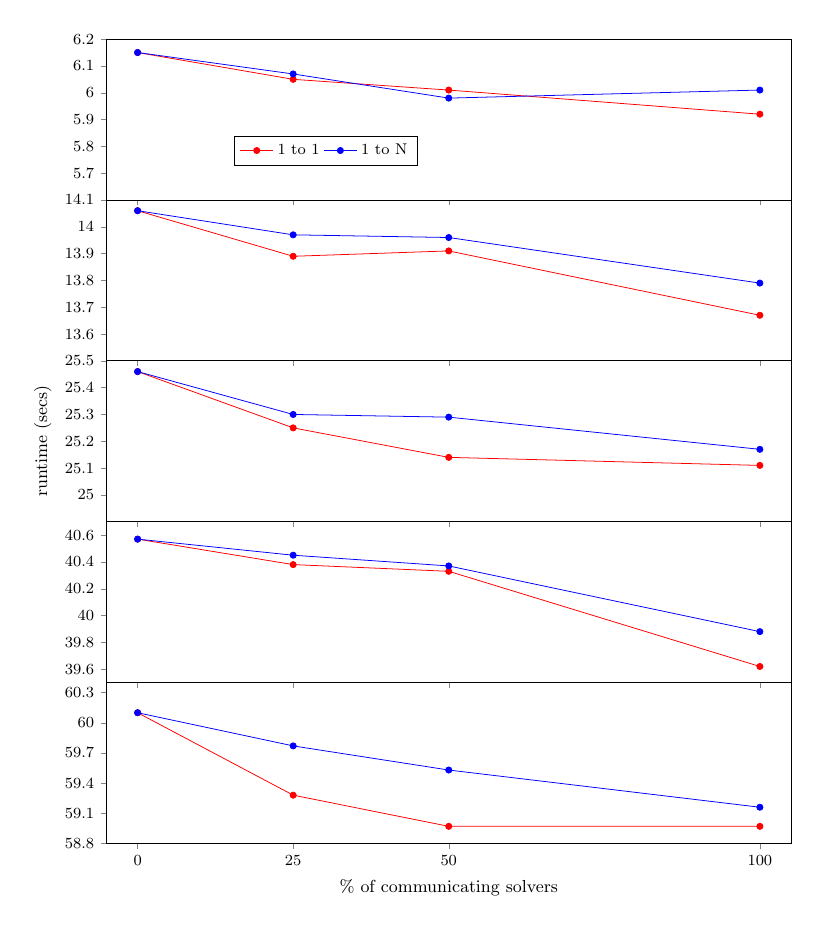
\begin{tikzpicture} [scale=0.7]
\begin{groupplot}[
group style={
	group name=my plots,
	group size=1 by 5,
	xlabels at=edge bottom,
	xticklabels at=edge bottom,		
	ylabels at=edge left,
	yticklabels at=edge left,
	vertical sep=0pt
},
legend style={at={(0.32,0.40)},anchor=north, legend columns=2},
footnotesize,
width=14cm,
height=4.5cm,
xlabel=\% of communicating solvers,
ylabel= \empty,
xmin=-5,
xmax=105,
ymin=0,	
ymax=30,
ytick={0,10,...,20},
xtick={0,25,50,100},
tickpos=left,
ytick align=outside,
xtick align=outside]

\nextgroupplot %2000
[ymin=5.6, ymax=6.2, ytick={5.7,5.8,5.9,6.0,6.1,6.2}, cycle list ={{red, mark options={fill=red,scale=0.8},mark=*}, {blue, mark options={fill=blue,scale=0.8},mark=*}, {green, mark options={fill=green,scale=0.8},mark=*}, {orange, mark options={fill=orange,scale=0.8},mark=x}}]
\addlegendentry{1 to 1}
\addplot coordinates{(0,6.15) (25,6.05) (50,6.01) (100,5.92)};
\addlegendentry{1 to N}
\addplot coordinates{(0,6.15) (25,6.07) (50,5.98) (100,6.01)};

\nextgroupplot %3000
[ymin=13.5, ymax=14.1, ytick={13.6,13.7,13.8,13.9,14.0,14.1}, cycle list ={{red, mark options={fill=red,scale=0.8},mark=*}, {blue, mark options={fill=blue,scale=0.8},mark=*}, {green, mark options={fill=green,scale=0.8},mark=*}, {orange, mark options={fill=orange,scale=0.8},mark=x}}]
\addplot coordinates{(0,14.06) (25,13.89) (50,13.91) (100,13.67)};
\addplot coordinates{(0,14.06) (25,13.97) (50,13.96) (100,13.79)};

\nextgroupplot %4000
[ymin=24.9, ymax=25.5, ytick={25.0,25.1,25.2,25.3,25.4,25.5}, cycle list ={{red, mark options={fill=red,scale=0.8},mark=*}, {blue, mark options={fill=blue,scale=0.8},mark=*}, {green, mark options={fill=green,scale=0.8},mark=*}, {orange, mark options={fill=orange,scale=0.8},mark=x}}, ylabel= runtime (secs)]
\addplot coordinates{(0,25.46) (25,25.25) (50,25.14) (100,25.11)};
\addplot coordinates{(0,25.46) (25,25.30) (50,25.29) (100,25.17)};

\nextgroupplot %5000
[ymin=39.5, ymax=40.7, ytick={39.6,39.8,40.0,40.2,40.4,40.6}, cycle list ={{red, mark options={fill=red,scale=0.8},mark=*}, {blue, mark options={fill=blue,scale=0.8},mark=*}, {green, mark options={fill=green,scale=0.8},mark=*}, {orange, mark options={fill=orange,scale=0.8},mark=x}}]
\addplot coordinates{(0,40.57) (25,40.38) (50,40.33) (100,39.62)};
\addplot coordinates{(0,40.57) (25,40.45) (50,40.37) (100,39.88)};

\nextgroupplot %6000
[ymin=58.8, ymax=60.4, ytick={58.8,59.1,59.4,59.7,60.0,60.3}, cycle list ={{red, mark options={fill=red,scale=0.8},mark=*}, {blue, mark options={fill=blue,scale=0.8},mark=*}, {green, mark options={fill=green,scale=0.8},mark=*}, {orange, mark options={fill=orange,scale=0.8},mark=x}}]
\addplot coordinates{(0,60.10) (25,59.28) (50,58.97) (100,58.97)};
\addplot coordinates{(0,60.10) (25,59.77) (50,59.53) (100,59.16)};
		
\end{groupplot}
\end{tikzpicture}
\caption[]{Runtime means of instances \\2000-, 3000-, 4000-, 5000- and 6000-queens}
\label{fig:results_nq}
\end{figure}

%----------------------------------------
%----- COSTAS
%---------------------------------------
\section{\carrp}

\modified{We present in Table~\ref{tab:costas17} results of launching {\it solver sets} to solve each instance of \carrp{} sequentially. Runtimes and iteration means showed in this Table are bigger than those presented in Table~\ref{tab:costas17comm}, confirming once again the success of the parallel approach.} %The column labeled \textbf{\% success} indicates the percentage of solvers that were able to find a solution before a time--out (5 minutes).

\begin{table}[h]
\captionsetup{belowskip=6pt,aboveskip=6pt}
\centering
\renewcommand{\arraystretch}{1}
\begin{tabular}{p{3.5cm}|R{1cm}R{1cm}R{1.2cm}R{1.2cm}R{2cm}}
	\hline
	{\bf STRATEGY} & T & T(ds) & It. & It.(sd) & \% success\\
	\hline
	%\hline
	Sequential (1 core) & 2.12 & 0.87 & 44,453 & 18,113 & 42.00\\
	Parallel (40 cores) & 0.73 & 0.46 & 9,556 & 6,439 & 100.00\\
	\hline
\end{tabular}
\caption{\carr{} 17: no communication}
\label{tab:costas17}
\end{table}

\modified{We chose directly the neighborhood module ($V_{AS}$), the selection module ($S_{First}$) and the acceptance module $A$, to create the solvers. We ran experiments to study parallel communicating strategies taken into account the structure of the communication, and the communication operator used, but in this problem, we perform the communication at two different times: at the time of applying the acceptance criteria, and at the time of performing the {\it reset}.}

\begin{table}
\centering 
\renewcommand{\arraystretch}{1}
\begin{tabular}{p{2.5cm}|R{1cm}R{1cm}R{1cm}R{1.2cm}|R{1cm}R{1cm}R{1cm}R{1.2cm}}
	\hline
	\multirow{3}{*}{\footnotesize{\centering {\bf STRATEGY}}} & \multicolumn{4}{c}{100\% COMM} & \multicolumn{4}{c}{50\% COMM} \\
	\cline{2-9}
	& T & T(sd) & It. & It.(sd) & T & T(sd) & It. & It.(sd)\\
	\hline
	Str A: 1 to 1 & \good{0.41} & 0.30 & 4,973 & 3,763 & 0.55 & 0.43 & 8,179 & 7,479\\
	Str A: 1 to N & 0.43 & 0.31 & 5,697 & 4,557 & 0.57 & 0.46 & 8,420 & 7,564\\	
	Str B: 1 to 1 & 0.48 & 0.41 & 6,546 & 5,562 & 0.51 & 0.49 & 8,004 & 7,998\\
	Str B: 1 to N & 0.45 & 0.46 & 5,701 & 6,295 & 0.48 & 0.51 & 7,245 & 8,379\\
	Str C: 1 to 1 & 0.48 & 0.43 & 6,954 & 6,706 & 0.58 & 0.43 & 8,329 & 6,593\\
	Str C: 1 to N & 0.49 & 0.38 & 6,457 & 5,875 & 0.58 & 0.50 & 8,077 & 8,319\\
	\hline
\end{tabular}
\caption{\carr{} 17: with communication}
\label{tab:costas17comm}
\end{table}

\modified{Table~\ref{tab:costas17comm} shows that the \as{} {\it A} (receiving the configuration at the time of applying the acceptance criteria) is more effective. The reason is that the others, interfere with the proper performance of the {\it reset}.} Table~\ref{tab:costas17comm} shows also high values of standard deviation. This is not surprising, due to the highly random nature of the neighborhood function and the selecting criterion, as well as the execution of many resets during the search process.

\section{\grp}

\modified{The benefit of the parallel approach is also proved for the \grp{} (see Table~\ref{tab:golomb_sec} w.r.t. \ref{tab:golomb_par_notabu}, \ref{tab:golomb_par_tabu}, \ref{tab:golomb_par_1-1} and \ref{tab:golomb_par_1-n}).} %The column labeled {\bf \%success} indicates the percentage of solvers that were able to find a solution before a time--out (5 minutes).

\modified{For \grp, the communication strategy that we adopt was different. Solvers do not communicate the current configuration to have more solvers searching in its neighborhood, but a configuration that we assume is a local minimum to be avoided. We consider that the current configuration is a local minimum since the solver (after a given number of iteration) is not able to find a better configuration in its neighborhood.}

\modified{The first experiment compares the runs of non communitaing solvers not using a {\it tabu} list with non communicating solvers using a {\it tabu} list. The results in Tables~\ref{tab:golomb_par_notabu} and \ref{tab:golomb_par_tabu} demonstrate that using a {\it tabu} list can help the search process. Without communication, the improvement is not substantial (8\% for 8--34, 7\% for 10--55 and 5\% for 11--72) because only one configuration is inserted in the \textit{tabu} list after each restart. \modified{When we use \textit{one to one} communication, after the restart $k$, the receiving solver has twice the number of configurations in the \textit{tabu} list (one {\it tabu} configuration from itself and the received one after each restart).} Table~\ref{tab:golomb_par_1-1} shows that this strategy is not sufficient for some instances, but when we use \textit{one to N} communication, the number of \textit{tabu} configurations after the restart $k$, in the receiving solver is considerably higher, e.g., after the restart $k$ a receiving solver has $k(N+1)$ configurations in his \textit{tabu} list. Hence, these solvers can generate configurations far enough from many potentially local minima. This phenomenon is more visible when the problem order increases. Table~\ref{tab:golomb_par_1-n} shows that the improvement for the higher case (11-72) is about 32\% w.r.t non communicating solvers not using a {\it tabu} list (Table~\ref{tab:golomb_par_notabu}), and about 29\% w.r.t non communicating solvers using a {\it tabu} list (Table~\ref{tab:golomb_par_tabu}).}

\begin{table}
	\captionsetup{belowskip=6pt,aboveskip=6pt}
	\centering 
	\renewcommand{\arraystretch}{1}
		\begin{tabular}{p{2cm}|R{1.2cm}R{1.2cm}|R{1.5cm}R{1.5cm}|R{0.8cm}R{1.2cm}|R{1.5cm}}
			\hline 	
			{\bf Instance} & T & T(sd) & It. & It.(sd) & R & R(sd) & \% success\\
			\hline
			%\hline
			8--34 & 0.79 & 0.66 & 13,306 & 11,154 & 66 & 55.74 & 100.00\\
			8--34 (t) & 0.66 & 0.63 & 10,745 & 10,259 & 53 & 51.35 & 100.00 \\
			10--55 & 66.44 & 49.56 & 451,419 & 336,858 & 301 & 224.56 & 80.00\\			
			10--55 (t) & 67.89 & 50.02 & 446,913 & 328,912 & 297 & 219.30 & 88.00\\
			11--72 & 160.34 & 96.11 & 431,623 & 272,910 & 143 & 90.91 & 26.67\\
			11--72 (t) & 117.49 & 85.62 & 382,617 & 275,747 & 127 & 91.85 & 30.00\\
			\hline
		\end{tabular}
	\caption{\gr: a single sequential solver}
	\label{tab:golomb_sec}
\end{table}

\begin{table}
	\captionsetup{belowskip=6pt,aboveskip=6pt}
	\centering 
	\renewcommand{\arraystretch}{1}
	\begin{tabular}{p{2cm}|R{1.2cm}R{1.2cm}|R{1.5cm}R{1.5cm}|R{0.8cm}R{1.2cm}}
		\hline 	
		{\bf Instance} & T & T(sd) & It. & It.(sd) & R & R(sd)\\
		\hline
		%\hline
		8--34 & 0.47 & 34.82 & 436 & 330.10 & 2 & 1.63\\
		10--55 & 5.31 & 38.63 & 22,577 & 16,488 & 15 & 11.00\\
		11--72 & 89.76 & 55.85 & 164,763 & 102,931 & 54 & 34.32\\
		\hline
	\end{tabular}
	\caption{\gr: parallel, without tabu list.}
	\label{tab:golomb_par_notabu}
\end{table}

\begin{table}
	\captionsetup{belowskip=6pt,aboveskip=6pt}
	\centering 
	\renewcommand{\arraystretch}{1}
	\begin{tabular}{p{2cm}|R{1.2cm}R{1.2cm}|R{1.5cm}R{1.5cm}|R{0.8cm}R{1.2cm}}
		\hline 	
		{\bf Instance} & T & T(sd) & It. & It.(sd) & R & R(sd)\\
		\hline
		%\hline
		8--34 & 0.43 & 0.37 & 349 & 334 & 1 & 1.64\\
		10--55 & 4.92 & 4.68 & 20,504 & 19,742 & 13 & 13.07\\
		11--72 & 85.02 & 67.22 & 155,251 & 121,928 & 51 & 40.64\\
		\hline
	\end{tabular}
	\caption{\gr: parallel, with tabu list.}
	\label{tab:golomb_par_tabu}
\end{table}

\begin{table}
	\captionsetup{belowskip=6pt,aboveskip=6pt}
	\centering 
	\renewcommand{\arraystretch}{1}
	\begin{tabular}{p{2cm}|R{1.2cm}R{1.2cm}|R{1.5cm}R{1.5cm}|R{0.8cm}R{1.2cm}}
		\hline 	
		{\bf Instance} & T & T(sd) & It. & It.(sd) & R & R(sd)\\
		\hline
		%\hline
		8--34 & 0.44 & 0.31 & 309 & 233 & 1 & 1.23\\
		10--55 & 3.90 & 3.22 & 15,437 & 12,788 & 10 & 8.52\\
		11--72 & 85.43 & 52.60 & 156,211 & 97,329 & 52 & 32.43\\
		\hline
	\end{tabular}
	\caption{\gr: parallel, communication 1 to 1.}
	\label{tab:golomb_par_1-1}
\end{table}

\begin{table}
	\captionsetup{belowskip=6pt,aboveskip=6pt}
	\centering 
	\renewcommand{\arraystretch}{1}
	\begin{tabular}{p{2cm}|R{1.2cm}R{1.2cm}|R{1.5cm}R{1.5cm}|R{0.8cm}R{1.2cm}}
		\hline 	
		{\bf Instance} & T & T(sd) & It. & It.(sd) & R & R(sd)\\
		\hline
		%\hline
		8--34 & 0.43 & 0.29 & 283 & 225 & 1 & 1.03\\
		10--55 & 3.16 & 2.82 & 12,605 & 11,405 & 8 & 7.61\\
		11--72 & 60.35 & 43.95 & 110,311 & 81,295 & 36 & 27.06\\
		\hline
	\end{tabular}
	\caption{\gr: parallel, communication 1 to n.}
	\label{tab:golomb_par_1-n}
\end{table}
%\part{Conclusions and future works}
%\chapter{Conclusion and future works}
\label{chap:conclusion}
\textit{In this chapter, the conclusions of this thesis is presented, emphasizing on our contribution and results. Future directions to follow are also discussed.}
\vfill
\minitoc
\newpage

\section{Conclusions}
\label{sec:conclusion_conclusion}

The era of parallel computing has opened new and more efficient ways to solve constrained problems. This development is leading us to the multi/many--core technology and massive parallel architectures, which are nowadays more accessible for a broad public through hardware like the Xeon Phi or GPU cards. For that reason, this new architecture implies new ways for designing and implementing algorithms to exploit its full potential.

In this thesis we have presented as a main contribution a Parallel-Oriented Solver Language (\posl) focused in the solution of \CSPs, which are very complicated. These problems have huge search spaces, making them intractable through tree-search techniques. \posl{} proposes a language to build meta-heuristic-based solvers, tacking into account the success of these methods solving \csps{}. These meta-heuristics are built using the \posl's language following rigorous but well detailed steps, based on the re-usability and coupling of small pieces of computation and communication (\oms{} and \opchs), designed for the resolution of a broad range of \csps. 

Meta-heuristic methods have some times a lot of parameters to be adjusted. Prior to the \posl{}'s design, Appendix~\ref{chap:prior_paramils} contains a study in which the tool {\sc ParamILS} was used to tune {\it Adaptive Search} to solve \carr{} and {\it All-Interval Series} problems. The main goals of that work was to study the performance of the tool, and to find a new and more efficient parameters setting allowing faster resolution of the mentioned benchmark problems. However, after a comparison between results obtained using default parameters found through manual experiments, and results obtained using {\sc ParamILS}, the conclusion was that, for this implementation of Adaptive Search, the tool is not suited to find parameter settings improving results using default parameters. This corroborates the practical intuition that, when the parameters set is not so large, the experience of the scientist is crucial and more accurate than using parameter tunning tools.

The most important characteristic of \posl{} is to allow the construction of many solvers to work in parallel using the \textit{multi-walk} approach. This has shown very good results solving constrained problems. Into another work prior to \posl's design, we have presented a study of some techniques to improve the performance of the algorithms proposed in \cite{Arbelaez2012} (\ie a study of the impact of space-partitioning techniques on the performance of parallel local search algorithms to tackle the \textit{K-Medoids Clustering Problem}). The basic idea of their specific problem is how to allocate communication metronodes in order to maximize the client covering. Their solution is based on domain partitioning techniques like {\it space-filling curves}, and {\it k-Means} algorithm, but they do not take into account the number of clients associated to each new sub-domain. For that reason, we proposed in Appendix~\ref{chap:prior_split} a set of ideas/hypothesis to improve the performance, using geometrical balancing of the search space. This work was not finished, because it was performed in parallel with the first ideas of \posl, which finally was the main direction of this thesis.

Chapter~\ref{chap:posl} was dedicated to \posl, the main contribution of this thesis, a Parallel-Oriented Solver Language to build
interconnected meta-heuristic-based solvers working in parallel. The language was formally presented by defining each provided operator, as well as the benchmark codification method, and the process of creation/usage of the \bothmodules. 

The most important advantage of \posl{} is to allow the codding, easily and fast, of many different solvers through a mechanism of module re-usability, and communication strategies through communication operators. Hence, as other contribution of this thesis, a detailed study of various communication strategies to analyze the behavior and relevance of the information sharing in solving constraint problems was presented in Chapter~\ref{chap:expe}.

An exploitation-oriented \commstr{} (in which the current configuration is communicated to focus various solvers in a more promising area) was successfully applied to the \sgp{}. The same idea was applied to solve the \nqp{}, showing no better results than without communication. However, a deep study of the \posl's behavior during the search process allows to design a \commstr{} able to improve the results of non-communicating strategies. It was based on crating \textit{companion} solvers (solvers only searching into a portion of the search space) to accelerate other's solvers search by communicating the current configuration. The cyclical exchange of this information shows good results for small instances. The \carrp{} is a very complicated constrained problem, and very sensitive to the methods to solve it. Thanks to some studies of different communication strategies, using the communication of the current configuration at different times (places) in the algorithm, it was possible to find a \commstr{} improving the performance obtained without communication. Finally, the \grp{} was chosen to study a different and innovative \commstr, in which the communicated information is a potential local minimum to be avoided. This new \commstr{} showed to be effective to solve these kinds of problems.

Using the operator-based language provided by \posl{} it was possible to test many different strategies either communicating or non-communicating. The process of building solvers implementing different solution strategies is complex and tedious, but \posl{} gives the possibility to make communicating and non-communicating solver prototypes and to study them with few efforts. It was possible to show that a good selection and management of inter-solvers communication can play an important role during the search process, for (most of them) very complicated constraint problems.

\section{Future works}

\posl{} is a tool entirely developed within the context of this thesis. It was completely new and yet under optimization. Although it has shown its first results, we believe that there is still a long way to go. 

One of the first steps to do when solving \CSPs{} using \posl{} is precisely the modeling problem. \posl{} (at the language level) does not provide a mechanism for benchmark modeling. It currently handles this issue through the low-level framework in C++ programing language, but the creation or integration of problem definition languages (\ie modeler) is one of the next goals.

During the resolution of \sgp{} the success of a \comstr{} combining intensification and exploration was showed. In that direction, many other strategies can be analyzed. For instance, the study of the cost history during the search process, in order to find a lower bound for the cost, that indicates when communicating the current configuration to all solvers. This strategy allows to focus the search in the same area by launching a generalized intensification.

%The \comstr{} applied to the resolution of \nqp{}, where \textit{partial solvers} transmit the configuration to \textit{full solvers}, accelerates the search process at the beginning. However, once the a configuration is accepted by a \textit{full solver}, \textit{partial solvers} are no longer able to find better configurations to be sent. The first idea coming into our minds is to create \textit{cyclic} \comstrs{} in which \textit{full solvers} return their improved configurations to \textit{partial solvers}. This way the search process can be accelerated at various moments. 

One of the most costly process during the resolution of \grp{} was to find the right {\it parameters} for the \textit{tabu list}. \new{A set of values showing the best behavior for each parameter was proposed after a tuning process.} Nevertheless, it is clear that in this part there is a lot of room for improvement. The key of the good performance of this strategy is the right election of the proximity criterion between configurations. For that reason this issue deserves a deep study in the future.

\posl{} already has an important library of ready--to--use computation and connection modules, based on a deep study of classical meta-heuristics algorithms for solving combinatorial problems. In the near future we plan to make it grow in order to increase possibilities of \posl{}. In such a way, building new algorithms by using \posl{} will be easier. At the same time we plan to enrich the language by proposing new operators. It is necessary, for example, to improve the solver definition language, allowing to build sets of many new solvers faster and easier. Furthermore, we aim at expanding the communication definition language in order to create versatile and more complex and dynamic communication strategies, and to allow dynamic communication strategies changing during runtime.

The operators described above only give the possibility to define static communication strategies. However, we aim to improve \posl{} with more expressive operators in terms of communication between solvers to allow dynamic modifications of communication strategies, that is, having such strategies adapting themselves during runtime. This way, many different communication strategies would be defined in the same \soset. \new{An example is to consider that we have defined some different conection's topologies in the same \commstr. Then, at some point, we aim to have the possibility of performing some evaluation of the search process, in order to turn the \commstr{} into one implementing the connection's topology which have obtained the best results. Furthermore, another perspective is to incorporate tools to obtain easily a valance between computation and communication, \ie a measure of the contribution of the communication with respect to performing, during the same amount of time, only calculation without communication.}

%Then, after some time of calculation, an evaluation would be performed in order to make all solvers able to adopt the best strategy until the end of the search process.

In most of the performed experiments, the shared information was the best found configuration. So far, there are no results showing what ``a good information to communicate'' is. Actually, \cite{Caniou14} shows that in fact, the current configuration is not always a relevant information to share among solvers. That is why this subject deserves a deep study. We plan in the near future to investigate other information to be communicated, such as search directions, and search space features, among others.

\posl{} provides a mechanism of sharing not only data (\ie configurations, neighborhoods, etc.) but also \oms{}. This is the most interesting characteristic of \posl{} but it was not possible to analyze it properly. With data exchange, solvers can expand or change their search zones. However, sharing \ms{} they can also mutate their behavior. In that sense, a future direction of this thesis proposes the study of other benchmark in order to find the right problem to successfully apply this approach.
%%----------------------------------------------------------------------------------------------
%------ RESULTS
%----------------------------------------------------------------------------------------------
\chapter{Analysis of results}
\label{chap:res}
\textit{In this chapter we explain the used environments were we run the experiments (description of my desktop machine, \textit{Curiosiphi} server, and eventually \textit{Grid5000}). We describe all the experiments and we expose a complete analysis of the obtained result.}
\vfill
\minitoc
\newpage

The experiments\footnote{\posl{} source code is available on GitHub:\href{https://github.com/alejandro-reyesamaro/POSL}{https://github.com/alejandro-reyesamaro/POSL}} 
were performed on an Intel\R{} Xeon\TM{} E5-2680 v2, 10$\times$4 cores, 2.80GHz. Results showed in this section are the means of 30 runs for each setup, presented in columns labeled {\bf T}, corresponding to the run-time in seconds, and {\bf It.} corresponding to the number of iterations; and their respective standard deviations ({\bf T(sd)} and {\bf It.(sd)}). In some tables, the column labeled \textbf{\% success} indicates the percentage of solvers finding a solution before reaching a time--out (5 minutes).

\modified{The experiments in this section are multi-walk runs using the same solver main structure (except differents w.r.t. communication operations). Parallel experiments use 40 cores for all problem instances.  It is important to point out that \posl{} is not designed to obtain the best results in terms of performance, but to give the possibility of rapidly prototyping and studying different cooperative or non cooperative search strategies.}

\section{\sgp}

We present in Table~\ref{tab:golfers_seq} results of launching \textit{solvers sets} to solve each instance of the problem sequentially. Not surprisingly, the means of sequential runtimes and iterations (Table~\ref{tab:golfers_seq}) are bigger than those means of parallel runs, with or without communication (all
other tables). 
%This confirms the intuition that parallel approach increases the probability of finding the solution within a more reasonable time (some tens of seconds), than with the sequential scheme \cite{Alon2011}. 
%The column labeled \textbf{\% success} in Table~\ref{tab:golfers_seq} indicates the percentage of solvers finding a solution before reaching a time--out (5 minutes). 
%presented in Table~\ref{tab:golfersB001}, column \textit{O.M. First Improvement} (without communication), and results with communication (Tables~\ref{tab:golfersB001comm100}, \ref{tab:golfersB001comm50} and \ref{tab:golfersB001comm25}). 


\begin{table}[h]
\centering
\renewcommand{\arraystretch}{1}
\begin{tabular}{p{1.5cm}|R{1.5cm}R{1.5cm}R{1.5cm}R{1.5cm}R{2.5cm}}
\hline
{\bf Instance} & T & T(sd) & It. & It.(sd) & \% success\\
\hline
%\hline
5--3--7 & 8.31 & 7.64 & 17,347 & 15,673 & 100.00\\
8--4--7 & 16.92 & 15.15 & 7,829 & 7,019 & 100.00\\
9--4--8 & 79.60 & 64.07 & 20,779 & 16,537 & 94.28\\
11--7--5 & 3.37 & 2.16 & 664 & 380 & 100.00\\
\hline
\end{tabular}
\caption{\sg: a single sequential solver}
\label{tab:golfers_seq}
\end{table}

In a first stage of the experiments we use the operator-based language provided by \posl{} to build and test many different non communicating strategies. The goal is to select the best concrete modules to run tests performing communication. In particular, we have tested two kind of computation modules: the one computing the neighborhood of a given configuration and the one choosing the current configuration for the next solver iteration.

We focused on choosing the right neighborhood function. In the case of the \sgp, this experiment was launched using a basic abstract solver showed in Algorithm~\ref{as:golfers10-10-3}.
%\footnote{\label{note:app3} Supplementary document {\it App[06-2016].pdf} (\href{https://goo.gl/W6W5VM}{https://goo.gl/W6W5VM})} 
Solvers implemented from this abstract solver was not able to solve instances beyond three weeks: they were very often trapped into local minima. This is the reason why we perform this first experiment with the instance 10--10--3 whereas next experiments scale above 3 weeks. This was not a problem though, since the goal of this first experiment was only to find the right concrete neighborhood module.

\begin{table}
\centering 
\renewcommand{\arraystretch}{1}
\begin{tabular}{p{4cm}|R{1.3cm}R{1.3cm}R{1.3cm}R{1.3cm}}
\hline
{\bf Abstract solvers} & T & T(sd) & It. & It.(sd) \\
\hline
%\hline
Adaptive Search (AS) & \good{\bf 1.06} & 0.79 & 352 & 268 \\		
Std $\circled{$\rho$}$ AS & 41.53 & 26.00 & 147 & 72\\
Std $\circled{$\cup$}$ AS & 59.65 & 55.01 & 198 & 110\\
Standard (Std) & 87.90 & 41.96 & 146 & 58 \\
\hline
\end{tabular}
\caption{\sg: Instance 10--10--3 in parallel}
\label{tab:golfers10-10-3}
\end{table}

Results in Table~\ref{tab:golfers10-10-3} are not surprising. The neighborhood neighborhood module $V_{AS}$ is based on the {\it Adaptive Search} algorithm, which has shown very good results \cite{Diaz}. %It selects the variable (player) contributing the most to the cost and permutes its value with the others variables (players) for all groups, every week.
It selects the most culprit variable (i.e. a player), that is, the variable to most responsible for constraints violation. Then, it permutes this variable value with the value of each other variable, in all groups and all weeks. Each permutation gives a neighbor of the current configuration. $V_{Std}$ uses no additional information, so it performs every possible swap between two players in different groups, every week. It means that this neighborhood is $g\times p$ times bigger than the previous one, with $g$ the number of groups and $p$ the number of players per group. We also tested abstract solvers with different combinations of these modules, using the $\circled{$\rho$}$ and the $\circled{$\cup$}$ operators. The $\circled{$\rho$}$ operator executes its first or second parameter depending on a given probability $\rho$, and the $\circled{$\cup$}$ operator returns the union of its parameters output. All these combinations spent more time searching the best configuration among the neighborhood, although with a lower number of iterations than $V_{AS}$. The $V_{AS}$ neighborhood function being clearly faster, we have chosen it for our experiments, even if it shown a more spread standard deviation: 0.75 for AS versus 0.62 for Std, considering the ratio $\tfrac{T(sd)}{T}$.

%It allows for more organized search because the set of neighbors is pseudo-deterministic, i.e., the construction criteria is always the same but the order of the configuration is random. On the other hand, {\it Adaptive Search} neighborhood function takes random decisions more frequently, and the order of the configurations is random as well. The AS neighborhood function being clearly faster, we selected it for our experiments. The combination using the operator $\circled{$\rho$}$ executes one or the other, depending on the probability $\rho$, and the combination using the operator $\circled{$\cup$}$ is the union of these neighborhoods. 

\begin{table}
\captionsetup{belowskip=6pt,aboveskip=6pt}
\centering 
\renewcommand{\arraystretch}{1}
\begin{tabular}{p{2cm}|R{1cm}R{1cm}R{1cm}R{1.2cm}|R{1cm}R{1cm}R{1cm}R{1.2cm}}
	\hline %\noalign{\smallskip}	
	\multirow{2}{*}{\footnotesize{\centering {\bf Instance}}} & 
	\multicolumn{4}{c|}{O.M. Best Improvement} & 
	\multicolumn{4}{c}{O.M. First Improvement}\\
	\cline{2-9} %\cline{3-8}
	& T & T(sd) & It. & It.(sd) & T & T(sd) & It. & It.(sd) \\
	\hline
	%\hline
	5--3--7 & 4.99 & 4.43 & 4,421 & 3,938 & \good{\bf 1.32} & 0.68 & 1322 & 676\\
	8--4--7 & 5.10 & 1.77 & 954 & 334 & \good{\bf 1.82} & 0.84 & 445 & 191\\	
	9--4--8 & 12.37 & 5.40 & 1,342 & 591 & \good{\bf 6.43} & 4.60 & 873 & 591 \\
	11--7--5 & 5.19 & 1.67 & 351 & 114 & \good{\bf 2.22} & 0.69 & 273 & 58\\
	\hline
\end{tabular}
\caption{\sg: comparing selection functions}
\label{tab:golfersB001}
\end{table}

With the selected neighborhood function, we focused on choosing the best {\it selection} function. We compared two different concrete modules used within the abstract solver in Algorithm~\ref{as:golfers_b001}, which combines selection modules ($S_{First}$ or $S_{Best}$) with $S_{Rand}$, to avoid being trapped into local minima: it tries to improve the cost in a limited number of iterations. If it is not possible, it selects a random neighbor for the next iteration. The first module was $S_{Best}$ that selects the best configuration inside the neighborhood. It not only spent more time searching a better configuration, but also is more sensitive to become trapped into local minima. The second module was $S_{First}$ which selects the first configuration inside the neighborhood improving the current cost. Using this module, solvers favor exploration over intensification and of course spend clearly less time computing the neighborhood. Table~\ref{tab:golfersB001} presents results of this experiment, showing that an exploration-oriented strategy is better for the {\it Social Golfers} problem. If we compare results of Tables~\ref{tab:golfers_seq} and \ref{tab:golfersB001} with respect to the standard deviation, we can some gains in robustness with parallelism. The spread in the running times and iterations for the instance 9--4--8 (the hardest one) is 10\% lower (0.80 sequentially versus 0.71 in parallel), and for the others, it is around 40\% lower (0.91, 0.89 and 0.64 sequentially versus 0.51, 0.45 and 0.31 in parallel, for 5--3--7, 8--4--7 and 11--7--5 respectively, with the same ratio $\tfrac{T(sd)}{T}$).

\begin{table}
	\captionsetup{belowskip=6pt,aboveskip=6pt}
	\centering 
	\renewcommand{\arraystretch}{1}
		\begin{tabular}{p{2cm}|R{1cm}R{1cm}R{1cm}R{1.2cm}|R{1cm}R{1cm}R{1cm}R{1.2cm}}
			\hline 	
			\multirow{2}{*}{\centering {\bf Instance}} & \multicolumn{4}{c}{Communication 1 to 1} & \multicolumn{4}{c}{Communication 1 to N}\\
			\cline{2-9}
			& T & T(sd) & It. & It.(sd) & T & T(sd) & It. & It.(sd) \\
			\hline
			%\hline
			5--3--7 & 1.19 & 0.64 & 1,156 & 608 & 1.11 & 0.49 & 1,067 & 484\\
			8--4--7 & \good{1.30} & 0.72 & \good{317} & 161 & 1.46 & 0.57 & 347 & 128\\
			9--4--8 & 4.38 & 2.72 & \good{597} & 347 & 5.51 & 3.06 & 736 & 389\\
			11--7--5 & 1.76 & 0.41 & 214 & 44 & \good{1.62} & 0.34 & \good{202} & 30\\
			\hline
		\end{tabular}
	\caption{\sg: test with 100\% of communication}
	\label{tab:golfersB001comm100}
\end{table}

\begin{table}
	\captionsetup{belowskip=6pt,aboveskip=6pt}
	\centering 
	\renewcommand{\arraystretch}{1}
		\begin{tabular}{p{2cm}|R{1cm}R{1cm}R{1cm}R{1.2cm}|R{1cm}R{1cm}R{1cm}R{1.2cm}}
			\hline 	
			\multirow{2}{*}{\centering {\bf Instance}} & \multicolumn{4}{c}{Communication 1 to 1} & \multicolumn{4}{c}{Communication 1 to N}\\
			\cline{2-9}
			& T & T(sd) & It. & It.(sd) & T & T(sd) & It. & It.(sd) \\
			\hline
			%\hline
			5--3--7 & 1.04 & 0.45 & 1,019 & 456 & 1.04 & 0.53 & 1,031 & 530\\
			8--4--7 & 1.40 & 0.57 & 337 & 122 & 1.43 & 0.76 & 353 & 167\\
			9--4--8 & 4.64 & 2.17 & 637 & 279 & 5.75 & 3.06 & 776 & 389 \\
			11--7--5 & 1.81 & 0.40 & 220 & 33 & 1.82 & 0.39 & 222 & 39\\
			\hline
		\end{tabular}
	\caption{\sg: test with 50 \% of communication}
	\label{tab:golfersB001comm50}
\end{table}

\begin{table}
	\captionsetup{belowskip=6pt,aboveskip=6pt}
	\centering 
	\renewcommand{\arraystretch}{1}
		\begin{tabular}{p{2cm}|R{1cm}R{1cm}R{1cm}R{1.2cm}|R{1cm}R{1cm}R{1cm}R{1.2cm}}
			\hline 	
			\multirow{2}{*}{\centering {\bf Instance}} & \multicolumn{4}{c}{Communication 1 to 1} & \multicolumn{4}{c}{Communication 1 to N}\\
			\cline{2-9}
			& T & T(sd) & It. & It.(sd) & T & T(sd) & It. & It.(sd) \\
			\hline
			%\hline
			5--3--7 & \good{0.90} & 0.51 & \good{881} & 492 & 1.19 & 0.67 & 1,170 & 655\\
			8--4--7 & 1.39 & 0.43 & 341 & 94 & 1.46 & 0.43 & 352 & 96\\
			9--4--8 & \good{4.33} & 1.92 & 599 & 248 & 4.53 & 2.01 & 625 & 251\\
			11--7--5 & 1.99 & 0.54 & 242 & 51 & 1.63 & 0.35 & 224 & 28 \\
			\hline
		\end{tabular}
	\caption{\sg: test with 25\% of communication}
	\label{tab:golfersB001comm25}
\end{table}

\modified{Then we ran experiments to study \posl's behavior solving target problems in communicating scenarios. Some compositions of solvers set were taken into account:}
\begin{inparaenum}[i.]
	\item the structure of the communication (with/without communication or a mix), and
	\item \modified{the used communication operator}.
\end{inparaenum}

Each time a \posl{} meta-solver is launched, many independent search solvers are executed. We call "good" configuration a configuration with the lowest cost within the current configuration neighborhood and with a cost strictly lesser than the current one. Once a good configuration is found in a sender solver, it is transmitted to the receiver one. At this moment, if the information is accepted, there are some solvers searching in the same subset of the search space, and the search process becomes more exploitation--oriented. This can be problematic if this process makes solvers converging too often towards local minima. In that case, we waste more than one solver trapped into a local minima: we waste all solvers that have been attracted to this part of the search space because of communications. We avoid this phenomenon through a simple (but effective) play: if a solver is not able to find a better configuration inside the neighborhood (executing $S_{First}$), it selects a random one at the next iteration (executing $S_{Rand}$). This strategy, using communication between solvers, produces some gain in terms of runtime (Table~\ref{tab:golfersB001} w.r.t. Tables~\ref{tab:golfersB001comm100}, \ref{tab:golfersB001comm50} and \ref{tab:golfersB001comm25}. The percentage of the receiver solvers that were able to find the solution before the others did, was significant \tet{See Anexes}. %(see tables in the supplementary documents)\footnote{\label{note:results} Supplementary document {\it Experiments[06-2016].ods}\\ (\href{https://goo.gl/QXAJeP}{https://goo.gl/rLqxuo})}. 
That shows that the communication played an important role during the search, despite inter--process communication's overheads (reception, information interpretation, making decisions, etc). For this problem we have reduced the spread in the running times and iterations of the results for the two last instances (9--4--8 and 11--7--5) applying the communication strategy (0.71 without communication versus 0.44 with communication, for 9--4--8, and 0.31 without communication versus 0.20 with communication for 11--7--5). %Having many solvers searching in different places of the search space, the probability that one of them reaches a promising place is higher. Then, when a solver finds a good configuration, it can be communicated, and receiving the help of one or more solvers in order to find the solution.

\section{\nqp}

\modified{We use directly the neighborhood module $V_{AS}$ based on the {\it Adaptive Search} algorithm, and the selection module $S_{First}$ which selects the first configuration inside the neighborhood improving the current cost, to create the solvers, and studying communicating and non communicating strategies.}

\begin{table}[h]
\centering 
\renewcommand{\arraystretch}{1}
\begin{tabular}{p{1.5cm}|R{2cm}R{2cm}|R{2cm}R{2cm}}
	\hline %\noalign{\smallskip}	
	\multirow{2}{*}{\footnotesize{\centering {\bf Instance}}} & \multicolumn{2}{c|}{\bf Sequential (1 core)} & \multicolumn{2}{c}{\bf No Comm. (40 cores)} \\
	\cline{2-5}
	& T & It. & T & It. \\	
	\hline
	2000 & & & 6.15 & 952 \\
	3000 & & & 14.06 & 1,413 \\
	4000 & & & 25.46 & 1,898 \\
	5000 & & & 40.57 & 2,377 \\
	6000 & & & 60.10 & 2,849 \\
	\hline
\end{tabular}
\caption{Results for \NQP{} (no communication)}\label{tab:nqueens_seq}
\end{table}

\begin{table}[h]
\centering 
\renewcommand{\arraystretch}{1}
\begin{tabular}{p{1.5cm}|R{1.5cm}R{1.5cm}|R{1.5cm}R{1.5cm}|R{1.5cm}R{1.5cm}}
	\hline %\noalign{\smallskip}	
	\multirow{2}{*}{\footnotesize{\centering {\bf Instance}}} & \multicolumn{2}{c|}{\bf 25\% Comm.} & \multicolumn{2}{c|}{\bf 50\% Comm.} &  \multicolumn{2}{c}{\bf All Comm.}\\
	\cline{2-7}
	& T & It. & T & It. & T & It. \\	
	\hline
	2000 &  6.05 & 934 & 6.01 & 920 & \good{\bf 5.92} & \good{\bf 885} \\
	3000 &  13.89 & 1,387 & 13.91 & 1,368 & \good{\bf 13.67} & \good{\bf 1,346}\\
	4000 & 25.26 & 1,868 & 25.14 & 1,855 & \good{\bf 25.11} & \good{\bf 1,834}\\
	5000 & 40.38 & 2,338 & 40.33 & 2,312 & \good{\bf 39.62} & \good{\bf 2,287}\\
	6000 & 59.28 & 2,794 & 58.97 & 2,775 & \good{\bf 58.97} & \good{\bf 2,729}\\	
	\hline
\end{tabular}
\caption{Results for \NQP{} (40 cores, communication 1~to~1)}\label{tab:nqueens_1to1}
\end{table}

\begin{table}[h]
\centering 
\renewcommand{\arraystretch}{1}
\begin{tabular}{p{1.5cm}|R{1.5cm}R{1.5cm}|R{1.5cm}R{1.5cm}|R{1.5cm}R{1.5cm}}
	\hline %\noalign{\smallskip}	
	\multirow{2}{*}{\footnotesize{\centering {\bf Instance}}} & \multicolumn{2}{c|}{\bf 25\% Comm.} & \multicolumn{2}{c|}{\bf 50\% Comm.} &  \multicolumn{2}{c}{\bf All Comm.}\\
	\cline{2-7}
	& T & It. & T & It. & T & It. \\	
	\hline
	2000 & 6.07 & 925 & \good{\bf 5.98} & 915 & 6.01 & \good{\bf 887}\\
	3000 & 13.97 & 1,402 & 13.96 & 1,386 & \good{\bf 13.79} & \good{\bf 1,365}\\
	4000 & 25.30 & 1,867 & 25.29 & 1,851 & \good{\bf 25.17} & \good{\bf 1,838}\\
	5000 & 40.45 & 2,338 & 40.37 & 2,312 & \good{\bf 39.88} & \good{\bf 2,291}\\
	6000 & 59.77 & 2,824 & 59.53 & 2,773 & \good{\bf 59.16} & \good{\bf 2,773}\\	
	\hline
\end{tabular}
\caption{Results for \NQP{} (40 cores, communication 1~to~N)}\label{tab:nqueens_1toN}
\end{table}

\modified{\posl{}, as we can see in Tables~\ref{tab:nqueens_1to1} and~\ref{tab:nqueens_1toN}, works very well without communication, for instances relatively big. This confirms once again the success of the \om{} $V_{AS}$ based on {\it Adaptive Search} algorithm to solve these kind of problems. The parallel approach outperforms significantly the sequential one, as we can see in Table~\ref{tab:nqueens_seq}. Runtimes and iteration means showed in this Table are bigger than those presented in Tables~\ref{tab:nqueens_1to1} and~\ref{tab:nqueens_1toN}. However, the communication improve the non communicating results in terms of runtime and iterations, this improvement is not significant. In contrast to \SGP, \posl{} does not get trapped so often into local minima during the resolution of \NQP{}. For that reason, the shared information, once received and accepted by the receivers solvers, does not improves largely the current cost.}

\modified{We can see the improvement with respect to the percentage of communicating solvers in Figure~\ref{fig:results_nq}. The bigger the instance is, the more significant the observed improvement is. This phenomenon suggests that a deeper study and an efficient implementation can make the communication playing a more significant role in the solution process.}

\pgfplotsset{
	myStyle/.style={grid=major,font=\Large}, ylabel= Communication rate,
	xlabel=Number of cores,
	legend style={at={(0.7,0.9)},
	anchor=north}
}

\begin{figure}
\centering
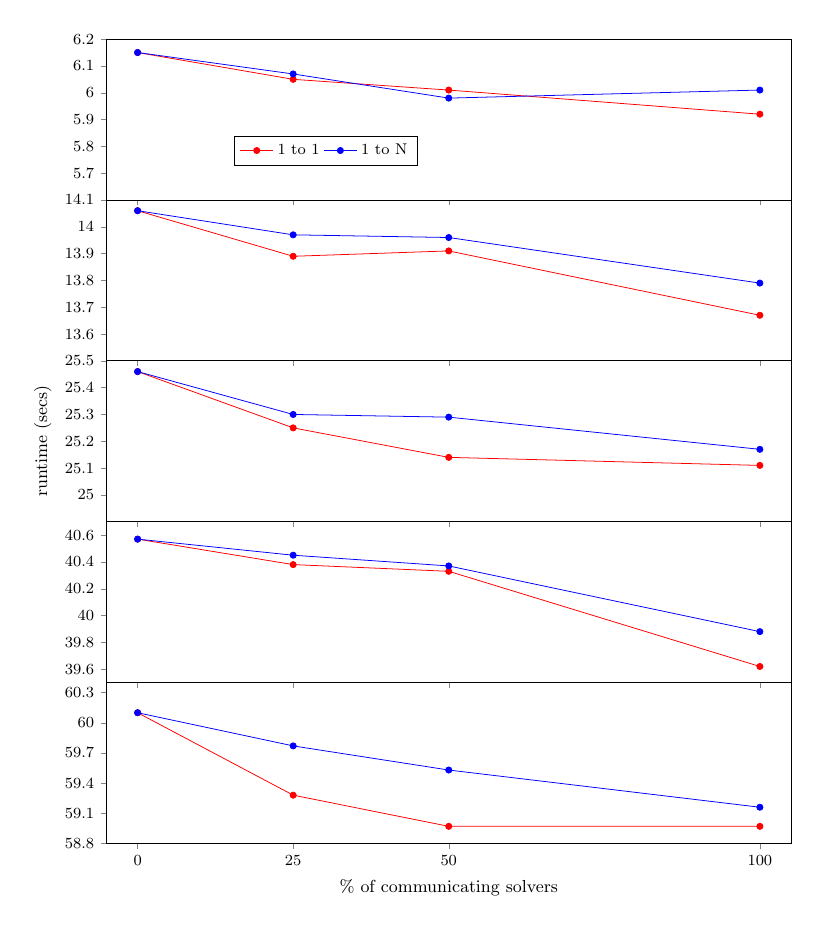
\begin{tikzpicture} [scale=0.7]
\begin{groupplot}[
group style={
	group name=my plots,
	group size=1 by 5,
	xlabels at=edge bottom,
	xticklabels at=edge bottom,		
	ylabels at=edge left,
	yticklabels at=edge left,
	vertical sep=0pt
},
legend style={at={(0.32,0.40)},anchor=north, legend columns=2},
footnotesize,
width=14cm,
height=4.5cm,
xlabel=\% of communicating solvers,
ylabel= \empty,
xmin=-5,
xmax=105,
ymin=0,	
ymax=30,
ytick={0,10,...,20},
xtick={0,25,50,100},
tickpos=left,
ytick align=outside,
xtick align=outside]

\nextgroupplot %2000
[ymin=5.6, ymax=6.2, ytick={5.7,5.8,5.9,6.0,6.1,6.2}, cycle list ={{red, mark options={fill=red,scale=0.8},mark=*}, {blue, mark options={fill=blue,scale=0.8},mark=*}, {green, mark options={fill=green,scale=0.8},mark=*}, {orange, mark options={fill=orange,scale=0.8},mark=x}}]
\addlegendentry{1 to 1}
\addplot coordinates{(0,6.15) (25,6.05) (50,6.01) (100,5.92)};
\addlegendentry{1 to N}
\addplot coordinates{(0,6.15) (25,6.07) (50,5.98) (100,6.01)};

\nextgroupplot %3000
[ymin=13.5, ymax=14.1, ytick={13.6,13.7,13.8,13.9,14.0,14.1}, cycle list ={{red, mark options={fill=red,scale=0.8},mark=*}, {blue, mark options={fill=blue,scale=0.8},mark=*}, {green, mark options={fill=green,scale=0.8},mark=*}, {orange, mark options={fill=orange,scale=0.8},mark=x}}]
\addplot coordinates{(0,14.06) (25,13.89) (50,13.91) (100,13.67)};
\addplot coordinates{(0,14.06) (25,13.97) (50,13.96) (100,13.79)};

\nextgroupplot %4000
[ymin=24.9, ymax=25.5, ytick={25.0,25.1,25.2,25.3,25.4,25.5}, cycle list ={{red, mark options={fill=red,scale=0.8},mark=*}, {blue, mark options={fill=blue,scale=0.8},mark=*}, {green, mark options={fill=green,scale=0.8},mark=*}, {orange, mark options={fill=orange,scale=0.8},mark=x}}, ylabel= runtime (secs)]
\addplot coordinates{(0,25.46) (25,25.25) (50,25.14) (100,25.11)};
\addplot coordinates{(0,25.46) (25,25.30) (50,25.29) (100,25.17)};

\nextgroupplot %5000
[ymin=39.5, ymax=40.7, ytick={39.6,39.8,40.0,40.2,40.4,40.6}, cycle list ={{red, mark options={fill=red,scale=0.8},mark=*}, {blue, mark options={fill=blue,scale=0.8},mark=*}, {green, mark options={fill=green,scale=0.8},mark=*}, {orange, mark options={fill=orange,scale=0.8},mark=x}}]
\addplot coordinates{(0,40.57) (25,40.38) (50,40.33) (100,39.62)};
\addplot coordinates{(0,40.57) (25,40.45) (50,40.37) (100,39.88)};

\nextgroupplot %6000
[ymin=58.8, ymax=60.4, ytick={58.8,59.1,59.4,59.7,60.0,60.3}, cycle list ={{red, mark options={fill=red,scale=0.8},mark=*}, {blue, mark options={fill=blue,scale=0.8},mark=*}, {green, mark options={fill=green,scale=0.8},mark=*}, {orange, mark options={fill=orange,scale=0.8},mark=x}}]
\addplot coordinates{(0,60.10) (25,59.28) (50,58.97) (100,58.97)};
\addplot coordinates{(0,60.10) (25,59.77) (50,59.53) (100,59.16)};
		
\end{groupplot}
\end{tikzpicture}
\caption[]{Runtime means of instances \\2000-, 3000-, 4000-, 5000- and 6000-queens}
\label{fig:results_nq}
\end{figure}

%----------------------------------------
%----- COSTAS
%---------------------------------------
\section{\carrp}

\modified{We present in Table~\ref{tab:costas17} results of launching {\it solver sets} to solve each instance of \carrp{} sequentially. Runtimes and iteration means showed in this Table are bigger than those presented in Table~\ref{tab:costas17comm}, confirming once again the success of the parallel approach.} %The column labeled \textbf{\% success} indicates the percentage of solvers that were able to find a solution before a time--out (5 minutes).

\begin{table}[h]
\captionsetup{belowskip=6pt,aboveskip=6pt}
\centering
\renewcommand{\arraystretch}{1}
\begin{tabular}{p{3.5cm}|R{1cm}R{1cm}R{1.2cm}R{1.2cm}R{2cm}}
	\hline
	{\bf STRATEGY} & T & T(ds) & It. & It.(sd) & \% success\\
	\hline
	%\hline
	Sequential (1 core) & 2.12 & 0.87 & 44,453 & 18,113 & 42.00\\
	Parallel (40 cores) & 0.73 & 0.46 & 9,556 & 6,439 & 100.00\\
	\hline
\end{tabular}
\caption{\carr{} 17: no communication}
\label{tab:costas17}
\end{table}

\modified{We chose directly the neighborhood module ($V_{AS}$), the selection module ($S_{First}$) and the acceptance module $A$, to create the solvers. We ran experiments to study parallel communicating strategies taken into account the structure of the communication, and the communication operator used, but in this problem, we perform the communication at two different times: at the time of applying the acceptance criteria, and at the time of performing the {\it reset}.}

\begin{table}
\centering 
\renewcommand{\arraystretch}{1}
\begin{tabular}{p{2.5cm}|R{1cm}R{1cm}R{1cm}R{1.2cm}|R{1cm}R{1cm}R{1cm}R{1.2cm}}
	\hline
	\multirow{3}{*}{\footnotesize{\centering {\bf STRATEGY}}} & \multicolumn{4}{c}{100\% COMM} & \multicolumn{4}{c}{50\% COMM} \\
	\cline{2-9}
	& T & T(sd) & It. & It.(sd) & T & T(sd) & It. & It.(sd)\\
	\hline
	Str A: 1 to 1 & \good{0.41} & 0.30 & 4,973 & 3,763 & 0.55 & 0.43 & 8,179 & 7,479\\
	Str A: 1 to N & 0.43 & 0.31 & 5,697 & 4,557 & 0.57 & 0.46 & 8,420 & 7,564\\	
	Str B: 1 to 1 & 0.48 & 0.41 & 6,546 & 5,562 & 0.51 & 0.49 & 8,004 & 7,998\\
	Str B: 1 to N & 0.45 & 0.46 & 5,701 & 6,295 & 0.48 & 0.51 & 7,245 & 8,379\\
	Str C: 1 to 1 & 0.48 & 0.43 & 6,954 & 6,706 & 0.58 & 0.43 & 8,329 & 6,593\\
	Str C: 1 to N & 0.49 & 0.38 & 6,457 & 5,875 & 0.58 & 0.50 & 8,077 & 8,319\\
	\hline
\end{tabular}
\caption{\carr{} 17: with communication}
\label{tab:costas17comm}
\end{table}

\modified{Table~\ref{tab:costas17comm} shows that the \as{} {\it A} (receiving the configuration at the time of applying the acceptance criteria) is more effective. The reason is that the others, interfere with the proper performance of the {\it reset}.} Table~\ref{tab:costas17comm} shows also high values of standard deviation. This is not surprising, due to the highly random nature of the neighborhood function and the selecting criterion, as well as the execution of many resets during the search process.

\section{\grp}

\modified{The benefit of the parallel approach is also proved for the \grp{} (see Table~\ref{tab:golomb_sec} w.r.t. \ref{tab:golomb_par_notabu}, \ref{tab:golomb_par_tabu}, \ref{tab:golomb_par_1-1} and \ref{tab:golomb_par_1-n}).} %The column labeled {\bf \%success} indicates the percentage of solvers that were able to find a solution before a time--out (5 minutes).

\modified{For \grp, the communication strategy that we adopt was different. Solvers do not communicate the current configuration to have more solvers searching in its neighborhood, but a configuration that we assume is a local minimum to be avoided. We consider that the current configuration is a local minimum since the solver (after a given number of iteration) is not able to find a better configuration in its neighborhood.}

\modified{The first experiment compares the runs of non communitaing solvers not using a {\it tabu} list with non communicating solvers using a {\it tabu} list. The results in Tables~\ref{tab:golomb_par_notabu} and \ref{tab:golomb_par_tabu} demonstrate that using a {\it tabu} list can help the search process. Without communication, the improvement is not substantial (8\% for 8--34, 7\% for 10--55 and 5\% for 11--72) because only one configuration is inserted in the \textit{tabu} list after each restart. \modified{When we use \textit{one to one} communication, after the restart $k$, the receiving solver has twice the number of configurations in the \textit{tabu} list (one {\it tabu} configuration from itself and the received one after each restart).} Table~\ref{tab:golomb_par_1-1} shows that this strategy is not sufficient for some instances, but when we use \textit{one to N} communication, the number of \textit{tabu} configurations after the restart $k$, in the receiving solver is considerably higher, e.g., after the restart $k$ a receiving solver has $k(N+1)$ configurations in his \textit{tabu} list. Hence, these solvers can generate configurations far enough from many potentially local minima. This phenomenon is more visible when the problem order increases. Table~\ref{tab:golomb_par_1-n} shows that the improvement for the higher case (11-72) is about 32\% w.r.t non communicating solvers not using a {\it tabu} list (Table~\ref{tab:golomb_par_notabu}), and about 29\% w.r.t non communicating solvers using a {\it tabu} list (Table~\ref{tab:golomb_par_tabu}).}

\begin{table}
	\captionsetup{belowskip=6pt,aboveskip=6pt}
	\centering 
	\renewcommand{\arraystretch}{1}
		\begin{tabular}{p{2cm}|R{1.2cm}R{1.2cm}|R{1.5cm}R{1.5cm}|R{0.8cm}R{1.2cm}|R{1.5cm}}
			\hline 	
			{\bf Instance} & T & T(sd) & It. & It.(sd) & R & R(sd) & \% success\\
			\hline
			%\hline
			8--34 & 0.79 & 0.66 & 13,306 & 11,154 & 66 & 55.74 & 100.00\\
			8--34 (t) & 0.66 & 0.63 & 10,745 & 10,259 & 53 & 51.35 & 100.00 \\
			10--55 & 66.44 & 49.56 & 451,419 & 336,858 & 301 & 224.56 & 80.00\\			
			10--55 (t) & 67.89 & 50.02 & 446,913 & 328,912 & 297 & 219.30 & 88.00\\
			11--72 & 160.34 & 96.11 & 431,623 & 272,910 & 143 & 90.91 & 26.67\\
			11--72 (t) & 117.49 & 85.62 & 382,617 & 275,747 & 127 & 91.85 & 30.00\\
			\hline
		\end{tabular}
	\caption{\gr: a single sequential solver}
	\label{tab:golomb_sec}
\end{table}

\begin{table}
	\captionsetup{belowskip=6pt,aboveskip=6pt}
	\centering 
	\renewcommand{\arraystretch}{1}
	\begin{tabular}{p{2cm}|R{1.2cm}R{1.2cm}|R{1.5cm}R{1.5cm}|R{0.8cm}R{1.2cm}}
		\hline 	
		{\bf Instance} & T & T(sd) & It. & It.(sd) & R & R(sd)\\
		\hline
		%\hline
		8--34 & 0.47 & 34.82 & 436 & 330.10 & 2 & 1.63\\
		10--55 & 5.31 & 38.63 & 22,577 & 16,488 & 15 & 11.00\\
		11--72 & 89.76 & 55.85 & 164,763 & 102,931 & 54 & 34.32\\
		\hline
	\end{tabular}
	\caption{\gr: parallel, without tabu list.}
	\label{tab:golomb_par_notabu}
\end{table}

\begin{table}
	\captionsetup{belowskip=6pt,aboveskip=6pt}
	\centering 
	\renewcommand{\arraystretch}{1}
	\begin{tabular}{p{2cm}|R{1.2cm}R{1.2cm}|R{1.5cm}R{1.5cm}|R{0.8cm}R{1.2cm}}
		\hline 	
		{\bf Instance} & T & T(sd) & It. & It.(sd) & R & R(sd)\\
		\hline
		%\hline
		8--34 & 0.43 & 0.37 & 349 & 334 & 1 & 1.64\\
		10--55 & 4.92 & 4.68 & 20,504 & 19,742 & 13 & 13.07\\
		11--72 & 85.02 & 67.22 & 155,251 & 121,928 & 51 & 40.64\\
		\hline
	\end{tabular}
	\caption{\gr: parallel, with tabu list.}
	\label{tab:golomb_par_tabu}
\end{table}

\begin{table}
	\captionsetup{belowskip=6pt,aboveskip=6pt}
	\centering 
	\renewcommand{\arraystretch}{1}
	\begin{tabular}{p{2cm}|R{1.2cm}R{1.2cm}|R{1.5cm}R{1.5cm}|R{0.8cm}R{1.2cm}}
		\hline 	
		{\bf Instance} & T & T(sd) & It. & It.(sd) & R & R(sd)\\
		\hline
		%\hline
		8--34 & 0.44 & 0.31 & 309 & 233 & 1 & 1.23\\
		10--55 & 3.90 & 3.22 & 15,437 & 12,788 & 10 & 8.52\\
		11--72 & 85.43 & 52.60 & 156,211 & 97,329 & 52 & 32.43\\
		\hline
	\end{tabular}
	\caption{\gr: parallel, communication 1 to 1.}
	\label{tab:golomb_par_1-1}
\end{table}

\begin{table}
	\captionsetup{belowskip=6pt,aboveskip=6pt}
	\centering 
	\renewcommand{\arraystretch}{1}
	\begin{tabular}{p{2cm}|R{1.2cm}R{1.2cm}|R{1.5cm}R{1.5cm}|R{0.8cm}R{1.2cm}}
		\hline 	
		{\bf Instance} & T & T(sd) & It. & It.(sd) & R & R(sd)\\
		\hline
		%\hline
		8--34 & 0.43 & 0.29 & 283 & 225 & 1 & 1.03\\
		10--55 & 3.16 & 2.82 & 12,605 & 11,405 & 8 & 7.61\\
		11--72 & 60.35 & 43.95 & 110,311 & 81,295 & 36 & 27.06\\
		\hline
	\end{tabular}
	\caption{\gr: parallel, communication 1 to n.}
	\label{tab:golomb_par_1-n}
\end{table}

\footnotesize
\bibliography{biblio201610}{} % Reference bib-library file
\bibliographystyle{unsrt}
\normalsize

%\appendix

%\part{Appendix}
%\chapter{Results of experiments with \sgp}
\label{app:sgp}
\textit{This Appendix presents graphically a summary of individuals runs using \sgp. Figures show a \textit{box-plot} representation for different strategies and a bar representation for the percentage of winner solvers types.}
\vfill
\newpage

\section{Comparison between sequential and parallel runs}

%Figures~\ref{subfig:boxplot_sel5}, \ref{subfig:boxplot_sel8} and \ref{subfig:boxplot_sel9} show the huge difference between the spread in results of sequential and parallel runs. Although both parallel strategies (best and first improvement) are equally stable, the one using the selection \om{} of first improvement shows better results: all of their runs are under the mean value of sequential runs (except a suspected outlier).
%
%\begin{figure}[!h]
%\centering
%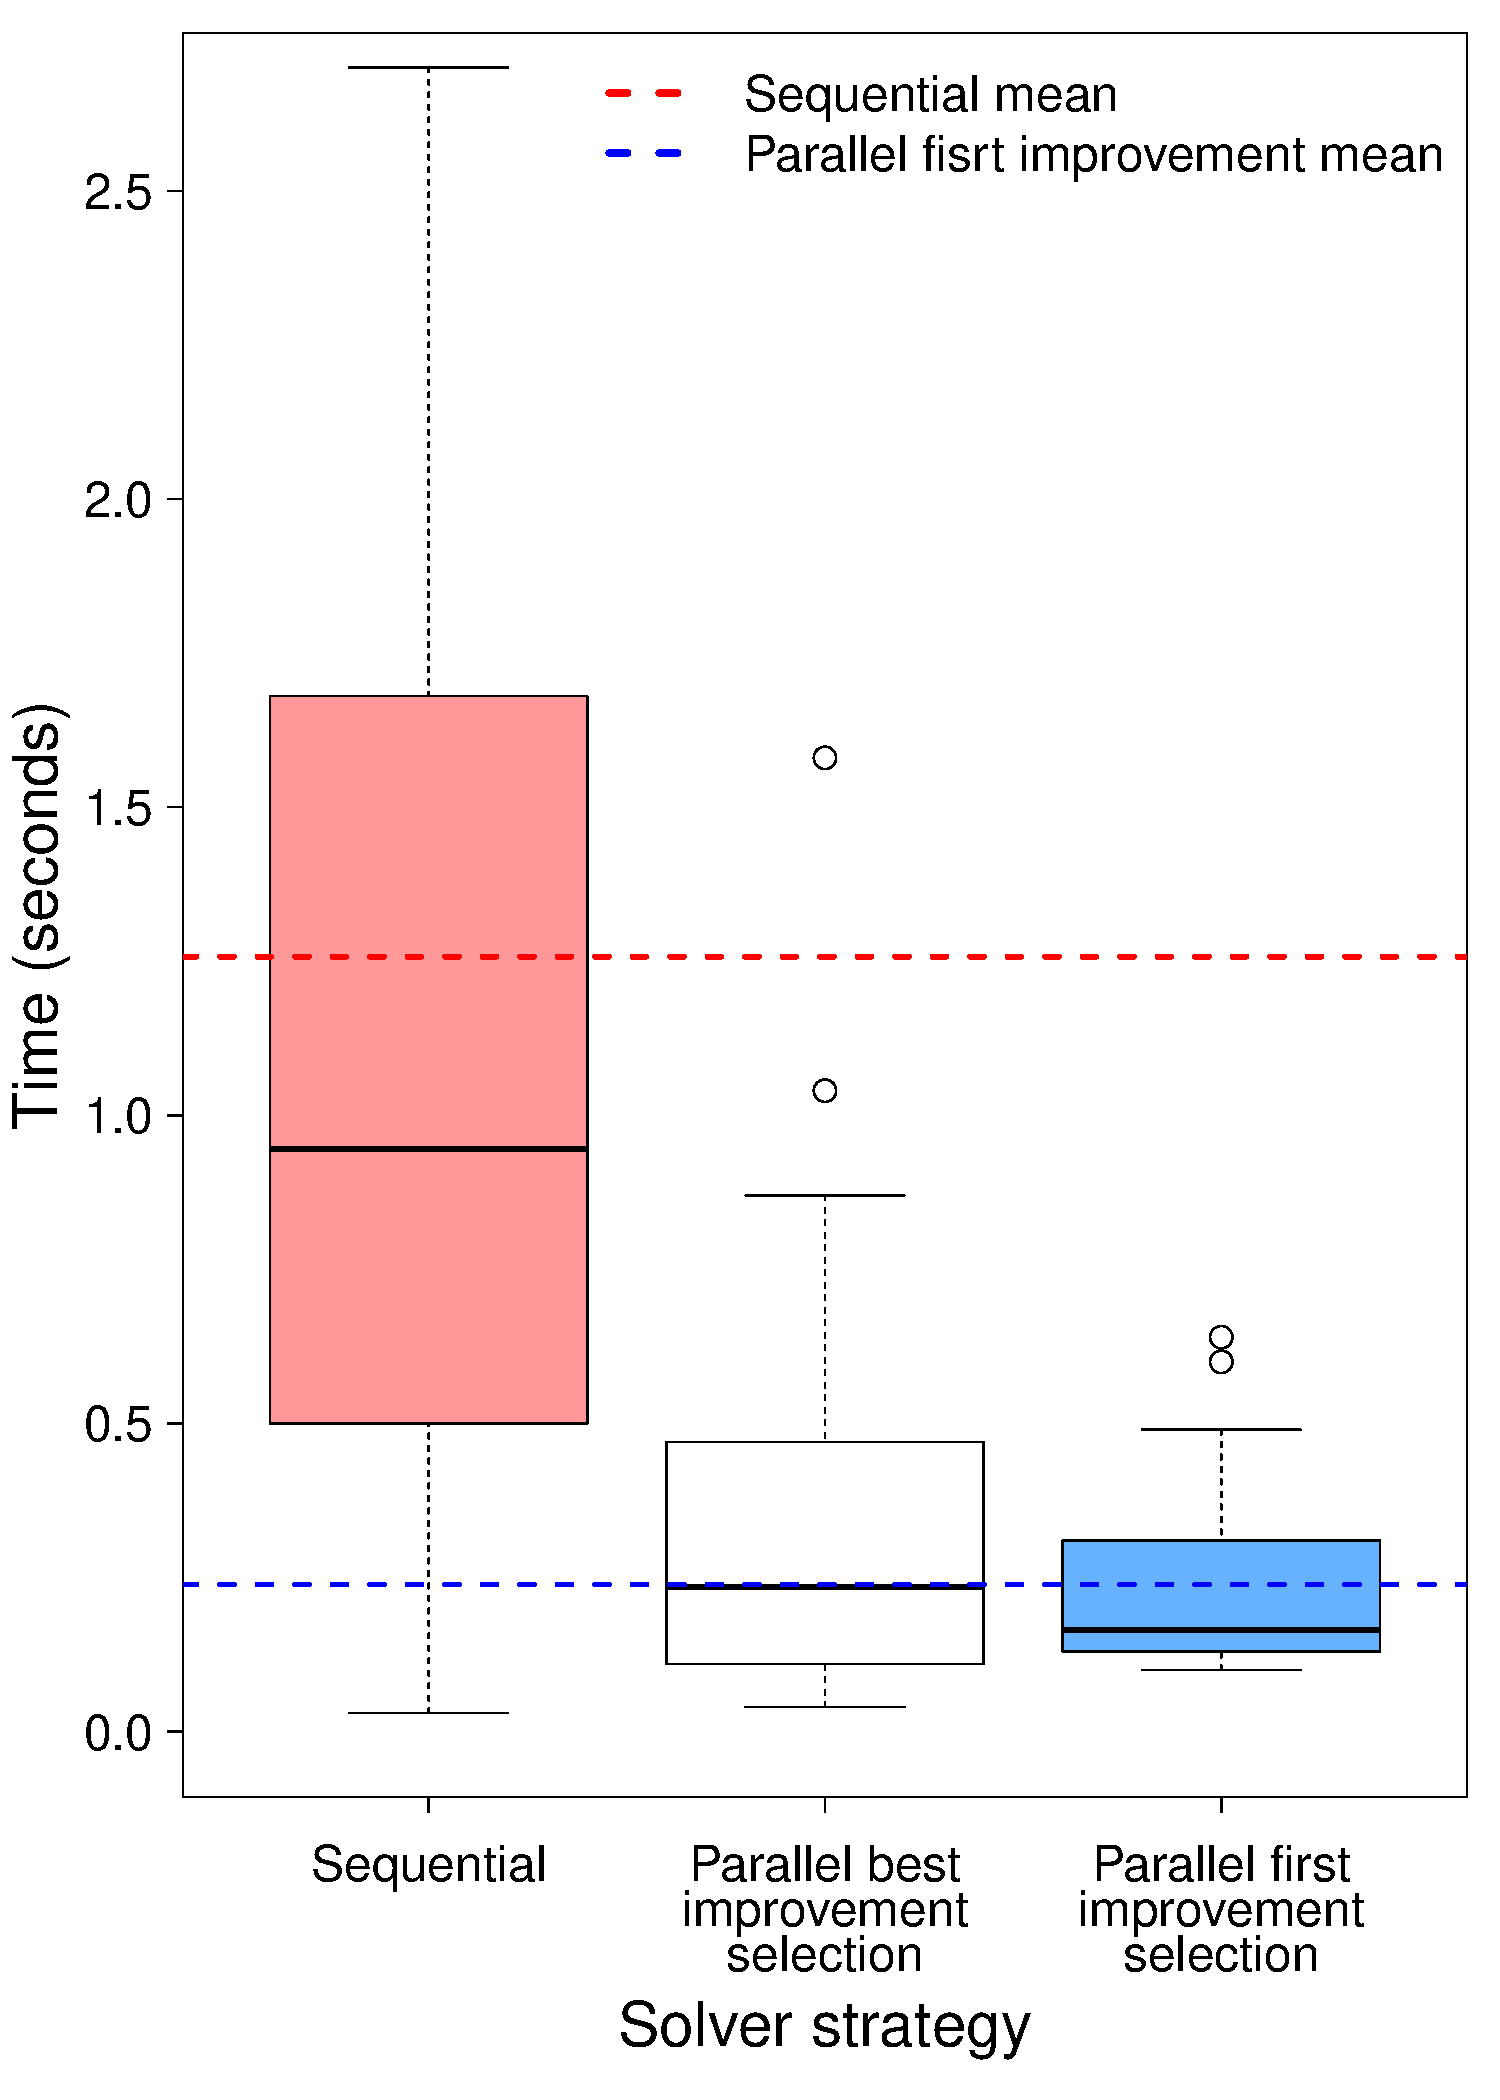
\includegraphics[width=0.4\linewidth]{g5_select_BP.pdf}
%\caption{Comparison between sequential and parallel (best improvement and first improvement selections) runs to solve \SGP{} 5-3-7 using \posl}\label{subfig:boxplot_sel5}
%\end{figure}

\begin{minipage}[c]{0.50\textwidth}
Figures~\ref{subfig:boxplot_sel5}, \ref{subfig:boxplot_sel8} and \ref{subfig:boxplot_sel9} show the huge difference between the spread in results of sequential and parallel runs. Although both parallel strategies (best and first improvement) are equally stable, the one using the selection \om{} of first improvement shows better results: all of their runs are under the mean value of sequential runs (except a suspected outlier).
\end{minipage}\hspace{0.05\textwidth}
\begin{minipage}[c]{0.40\textwidth}
\centering
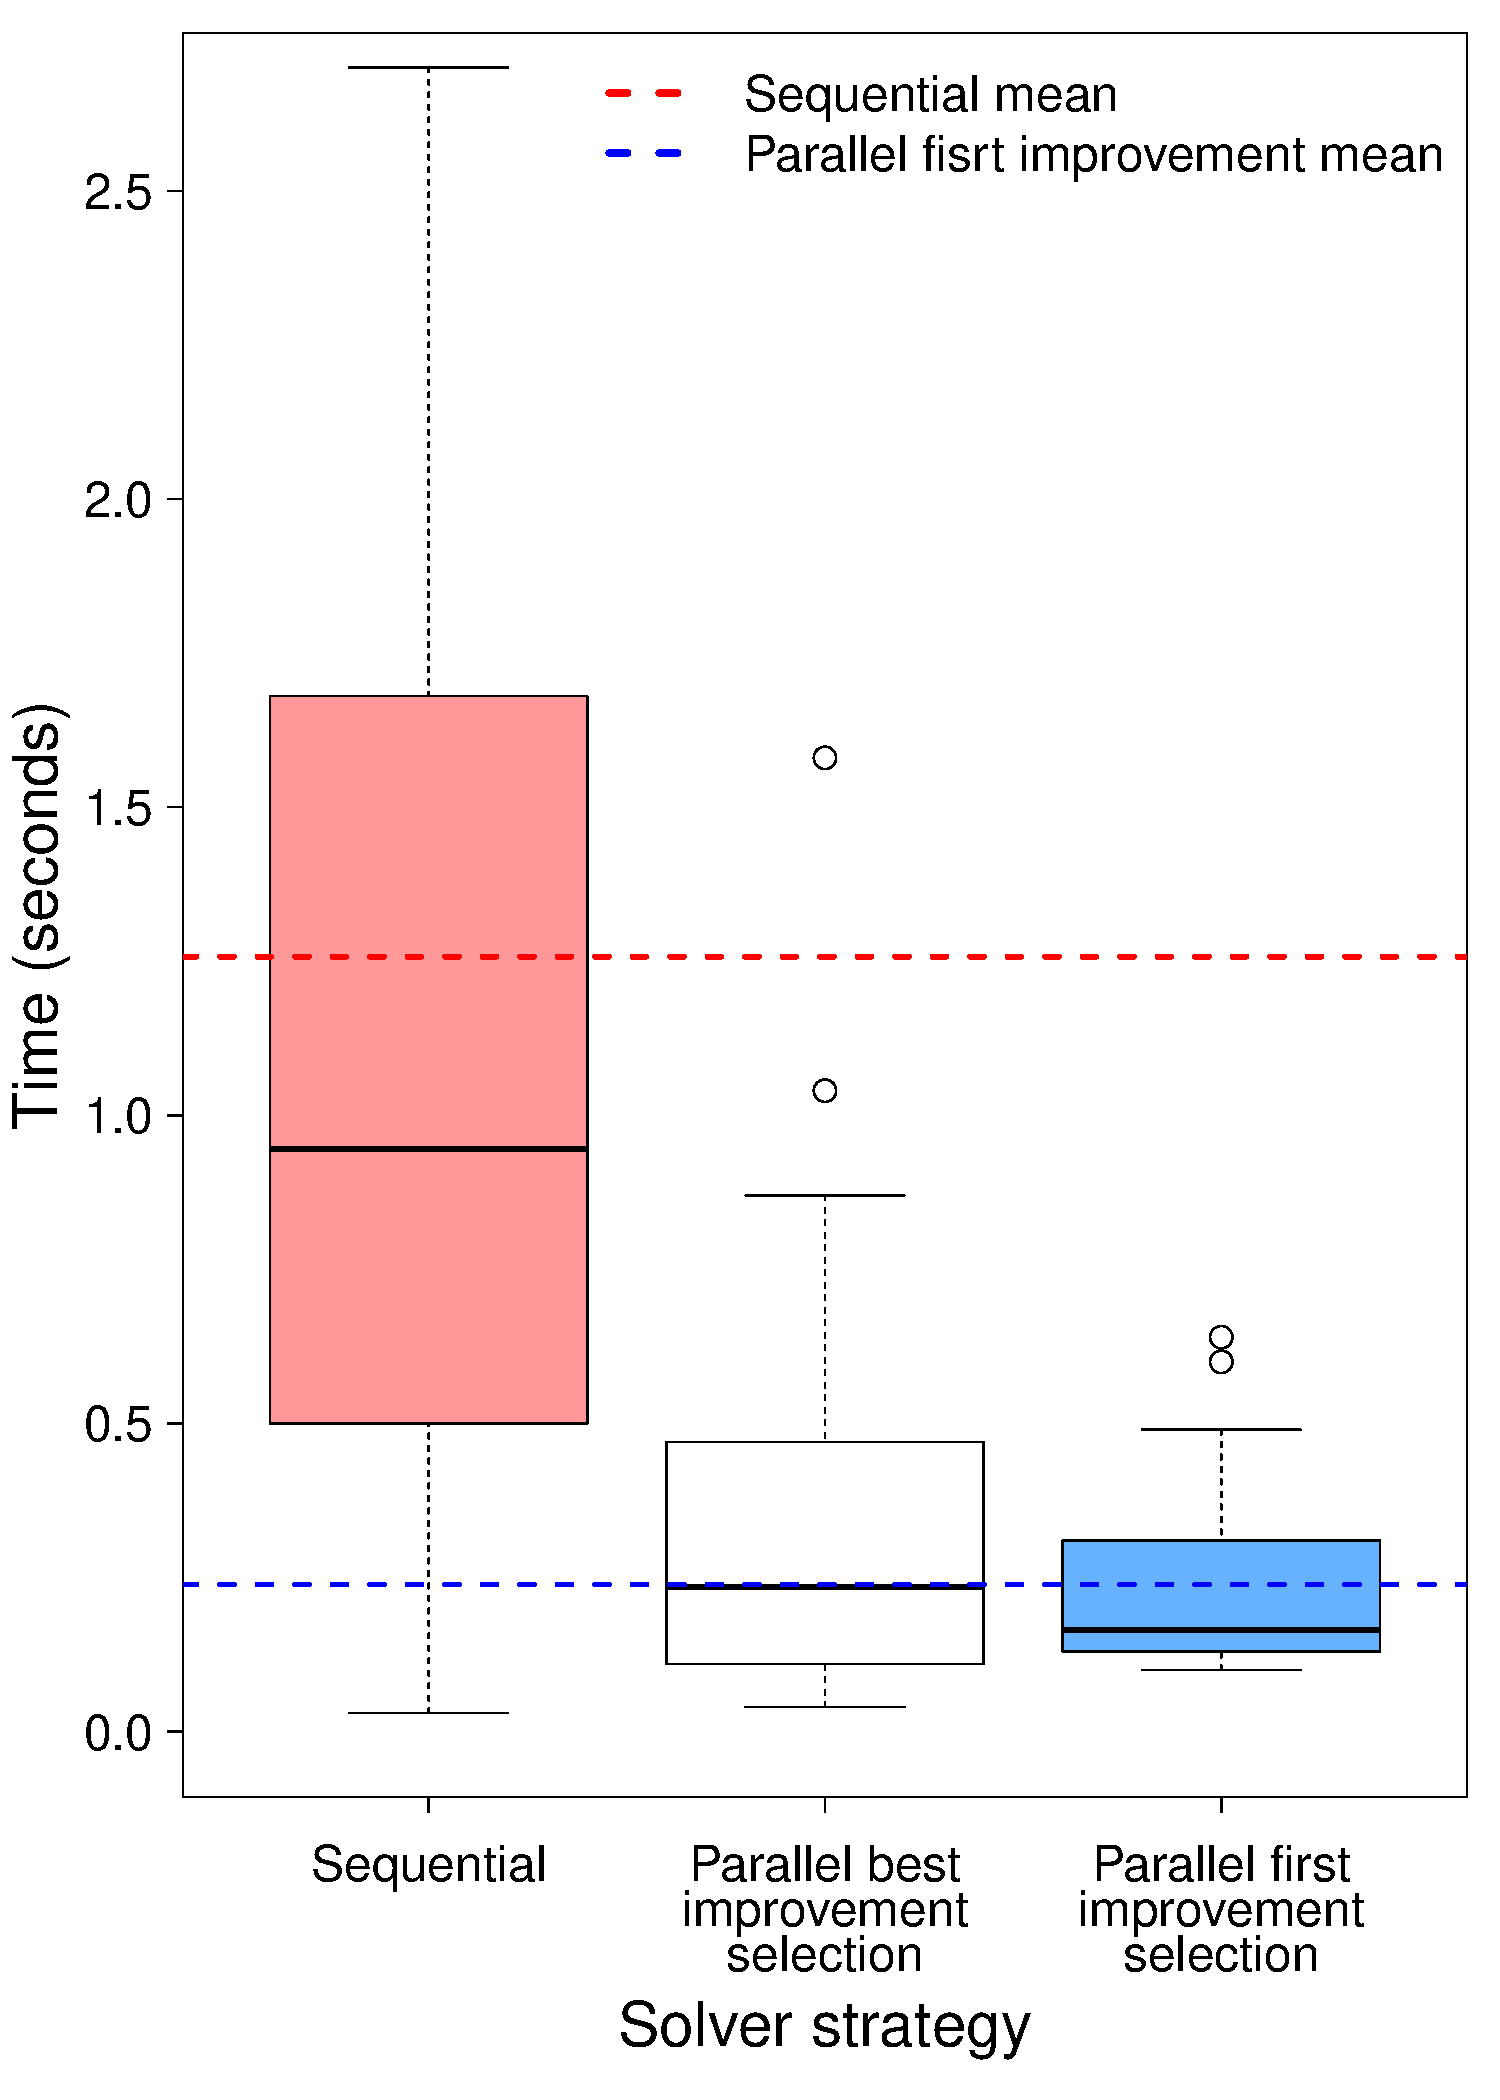
\includegraphics[width=0.9\linewidth]{g5_select_BP.pdf}
\captionof{figure}{Comparison between sequential and parallel (best improvement and first improvement selections) runs to solve \SGP{} 5-3-7 using \posl}\label{subfig:boxplot_sel5}
\end{minipage}

\begin{minipage}[c]{0.45\textwidth}
\centering
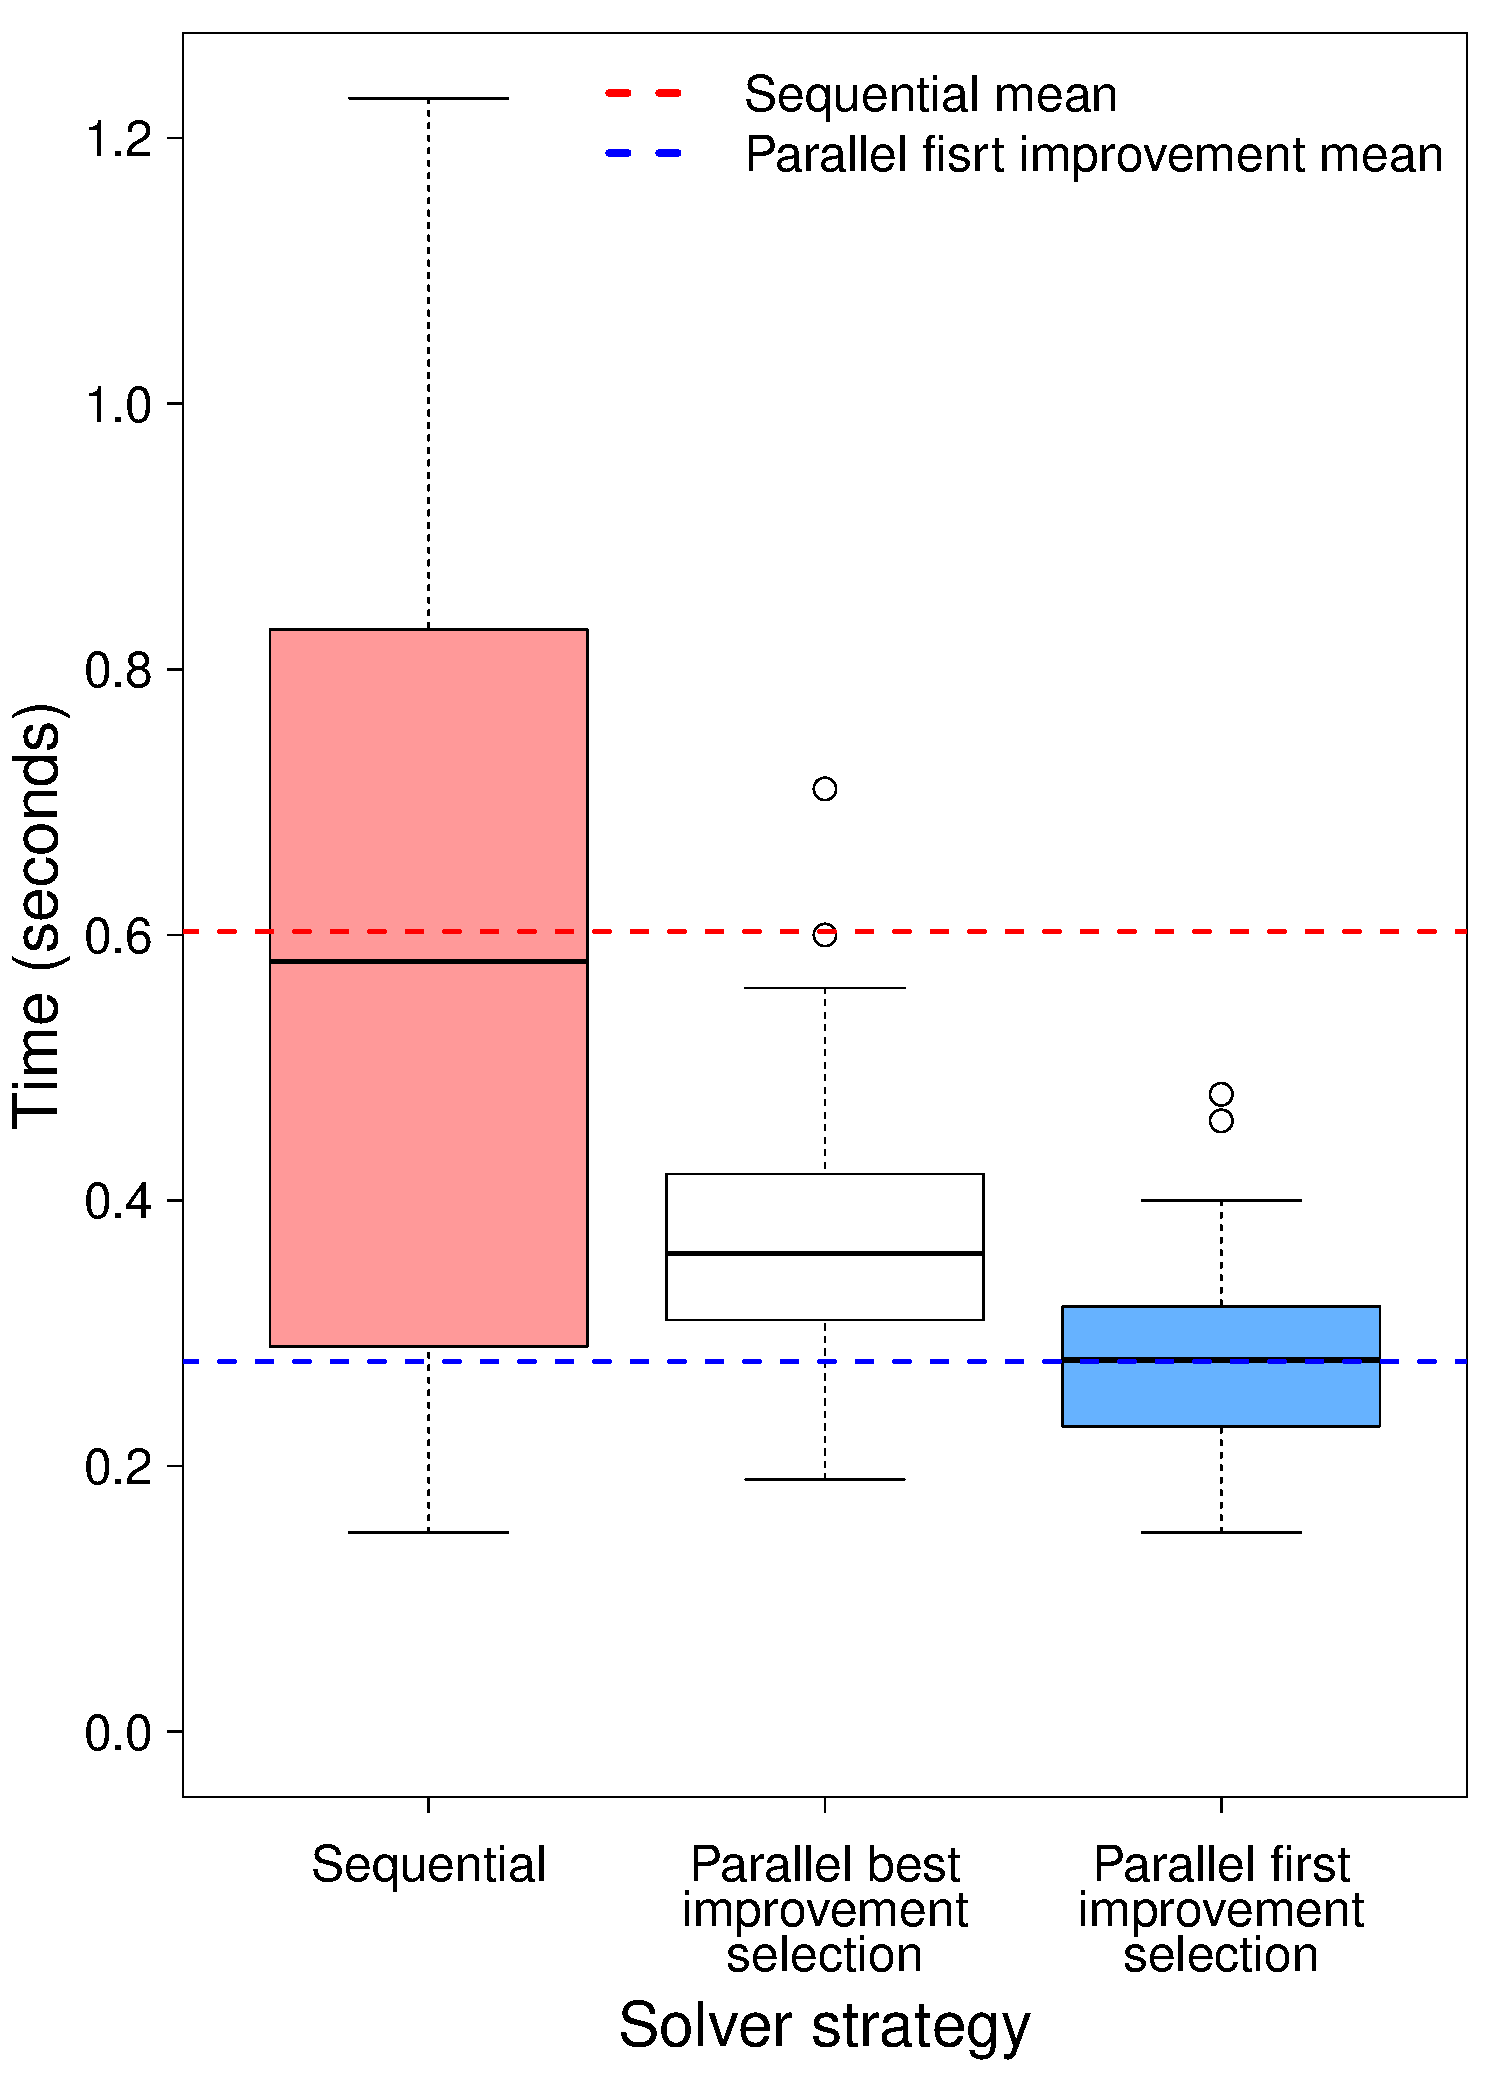
\includegraphics[width=\linewidth]{g8_select_BP.pdf}
\captionof{figure}{Comparison between sequential and parallel (best improvement and first improvement selections) runs to solve \SGP{} 8-4-7 using \posl}\label{subfig:boxplot_sel8}
\end{minipage}\hspace{0.05\textwidth}
\begin{minipage}[c]{0.45\textwidth}
\centering
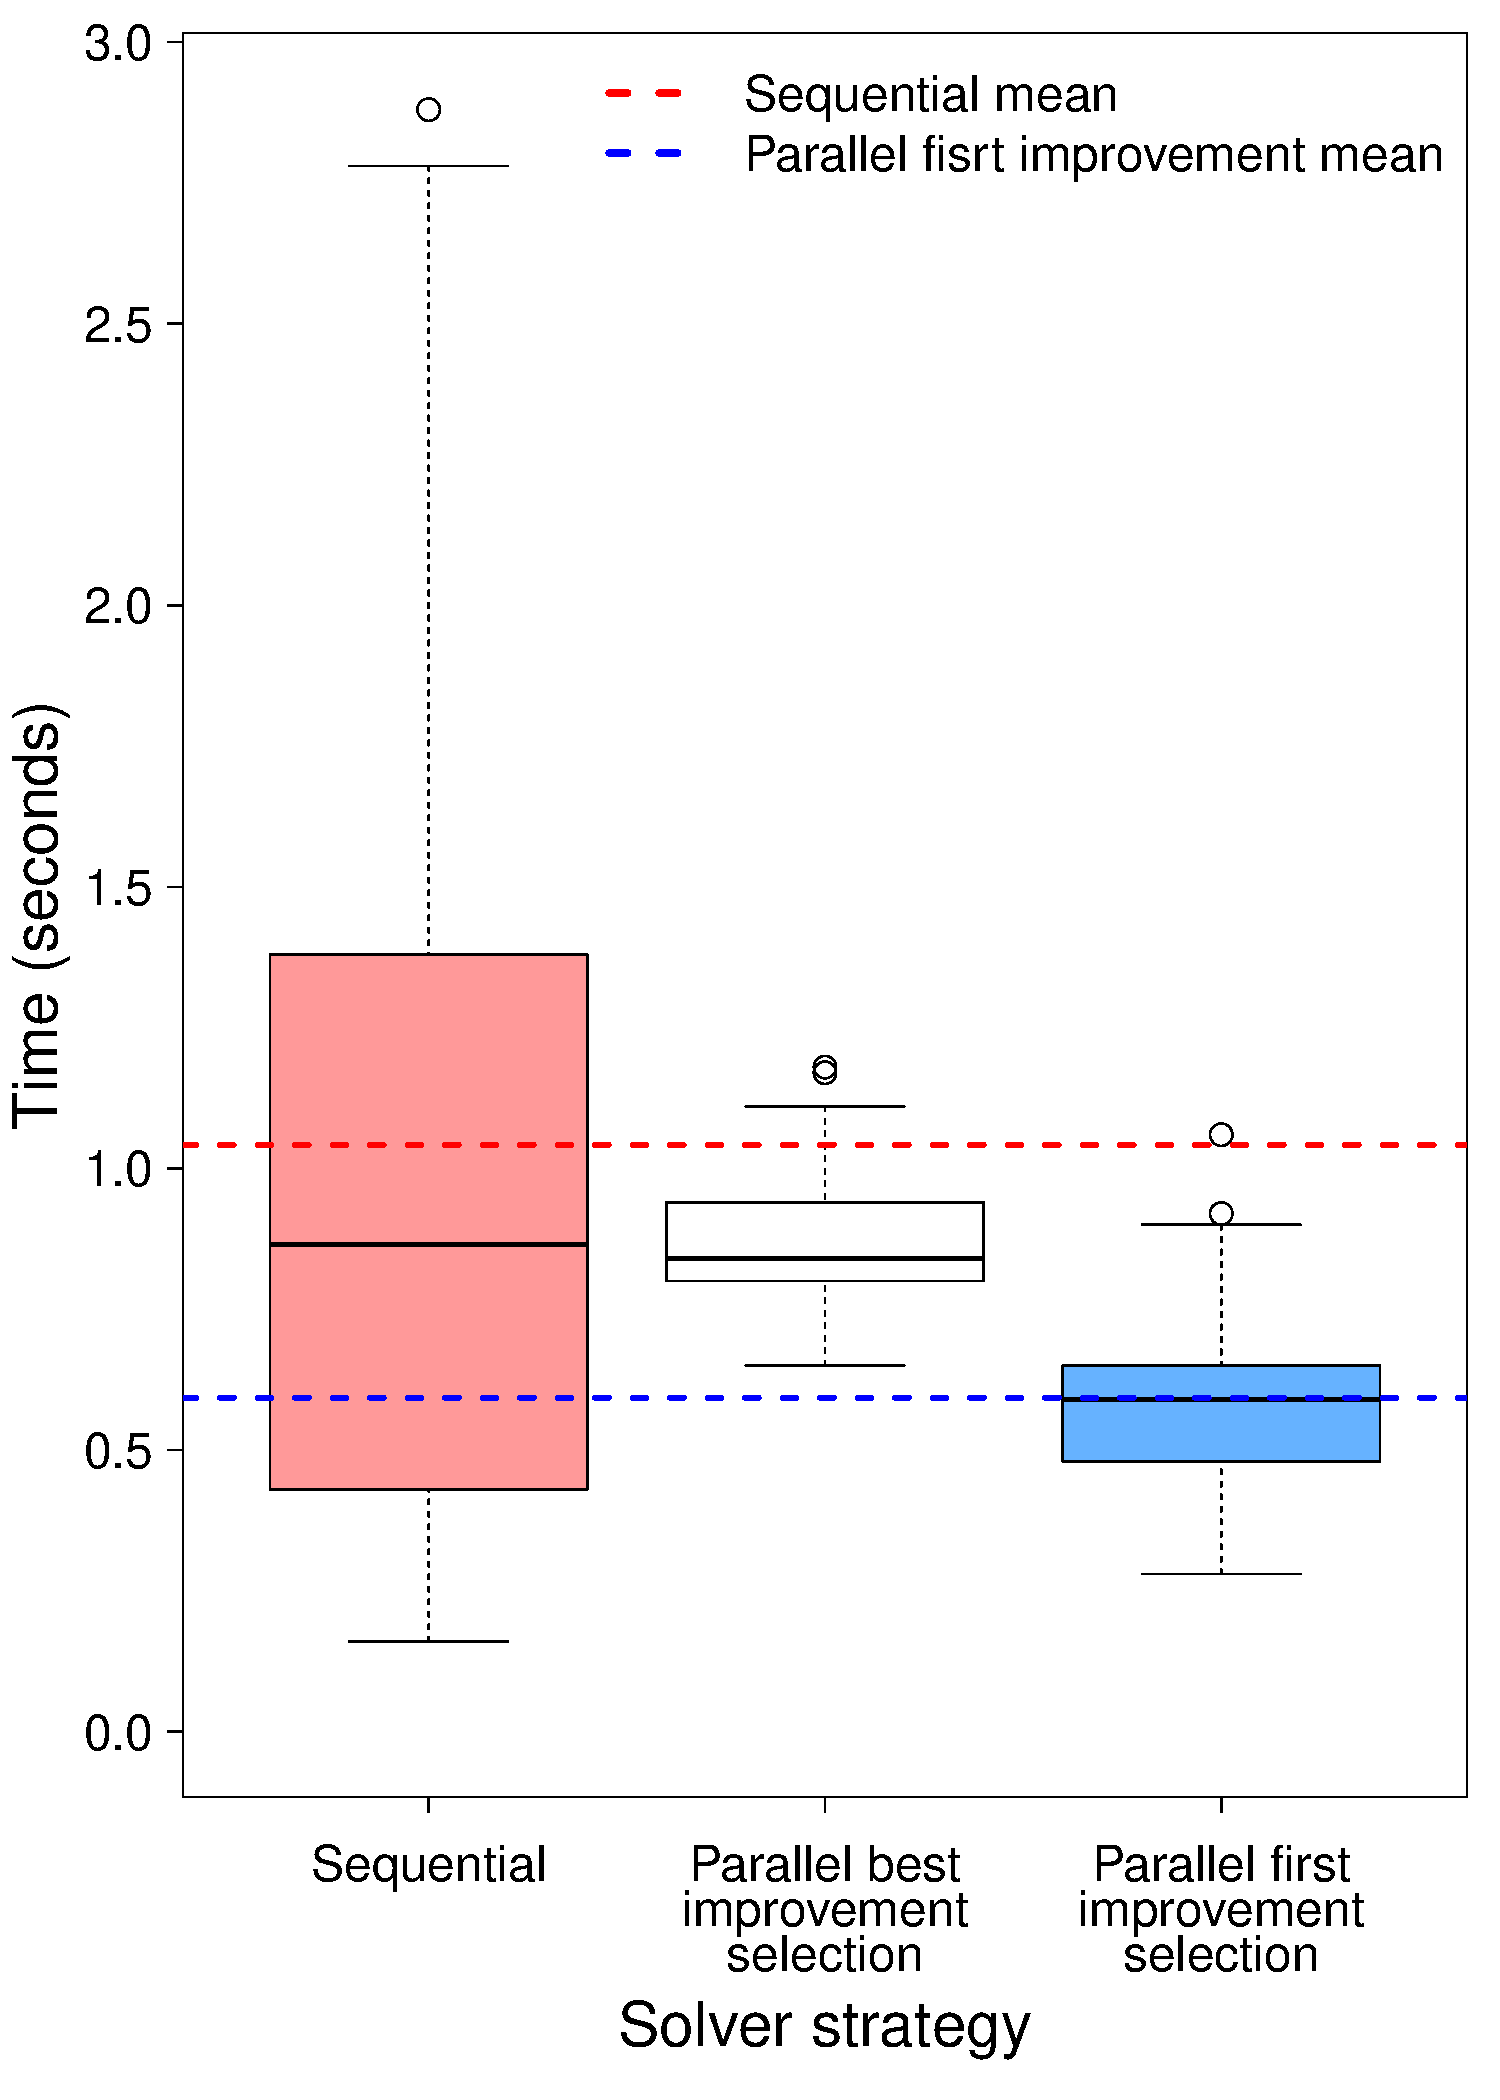
\includegraphics[width=\linewidth]{g9_select_BP.pdf}
\captionof{figure}{Comparison between sequential and parallel (best improvement and first improvement selections) runs to solve \SGP{} 9-4-8 using \posl}\label{subfig:boxplot_sel9}
\end{minipage}

\section{Comparison between \commstrs}

In Figures~\ref{boxplot:5comm}, \ref{boxplot:8comm} and \ref{boxplot:9comm}, labels of the x-axis correspond to the following strategies:

\poslcaptiondesciption{
\begin{tabular}[t]{rl}
\textbf{NC}: & \begin{tabular}[t]{l} Non communication strategy \end{tabular} \\
%\textbf{NC}: & Non communication strategy\\
\textbf{100SC1-1}: & \begin{tabular}[t]{l} 100\% of communicating solvers performing simple communication \oneTone \end{tabular} \\
\textbf{50SC1-1}: & \begin{tabular}[t]{l} 50\% of communicating solvers performing simple communication \oneTone \end{tabular} \\
\textbf{25SC1-1}: & \begin{tabular}[t]{l} 25\% of communicating solvers performing simple communication \oneTone \end{tabular} \\
\textbf{100SC1-n}: & \begin{tabular}[t]{l} 100\% of communicating solvers performing simple communication \oneTn \end{tabular} \\
\textbf{50SC1-n}: & \begin{tabular}[t]{l} 50\% of communicating solvers performing simple communication \oneTn \end{tabular} \\
\textbf{25SC1-n}: & \begin{tabular}[t]{l} 25\% of communicating solvers performing simple communication \oneTn \end{tabular}\\
\textbf{CC1-n}: & \begin{tabular}[t]{l} One set of solvers performing dynamic exchange communication \oneTn \end{tabular} \\
\textbf{CC1-n/2}: & \begin{tabular}[t]{l} Two sets of solvers performing dynamic exchange communication \oneTn \end{tabular} \\
\textbf{CC1-n/4}: & \begin{tabular}[t]{l} Four sets of solvers performing dynamic exchange communication \oneTn \end{tabular} \\
\textbf{100CC1-1}: & \begin{tabular}[t]{l} 100\% of communicating solvers performing dynamic exchange communication \\ \oneTone \end{tabular}\\
\textbf{50CC1-1}: & \begin{tabular}[t]{l} 50\% of communicating solvers performing dynamic exchange communication \\ \oneTone \end{tabular} \\
\textbf{25CC1-1}: & \begin{tabular}[t]{l} 25\% of communicating solvers performing dynamic exchange communication \\ \oneTone \end{tabular}\\
\end{tabular}
}

Figures~\ref{boxplot:5comm}, \ref{boxplot:8comm} and~\ref{boxplot:9comm} show results summaries of different \commstrs{}. They are presented together with the box-plot graph of parallel results without communication (\texttt{NC}). In all cases we can observe that strategies \texttt{100\%CC1-1} and \texttt{50\%CC1-1}  show excellent results in comparison to the one without communication. This figure shows also that simple \commstrs{} do not contribute enough to the improvement of the search time.

%------ COMMUNICATION
%\begin{figure}[h]
\begin{minipage}[c]{\textwidth}
\centering
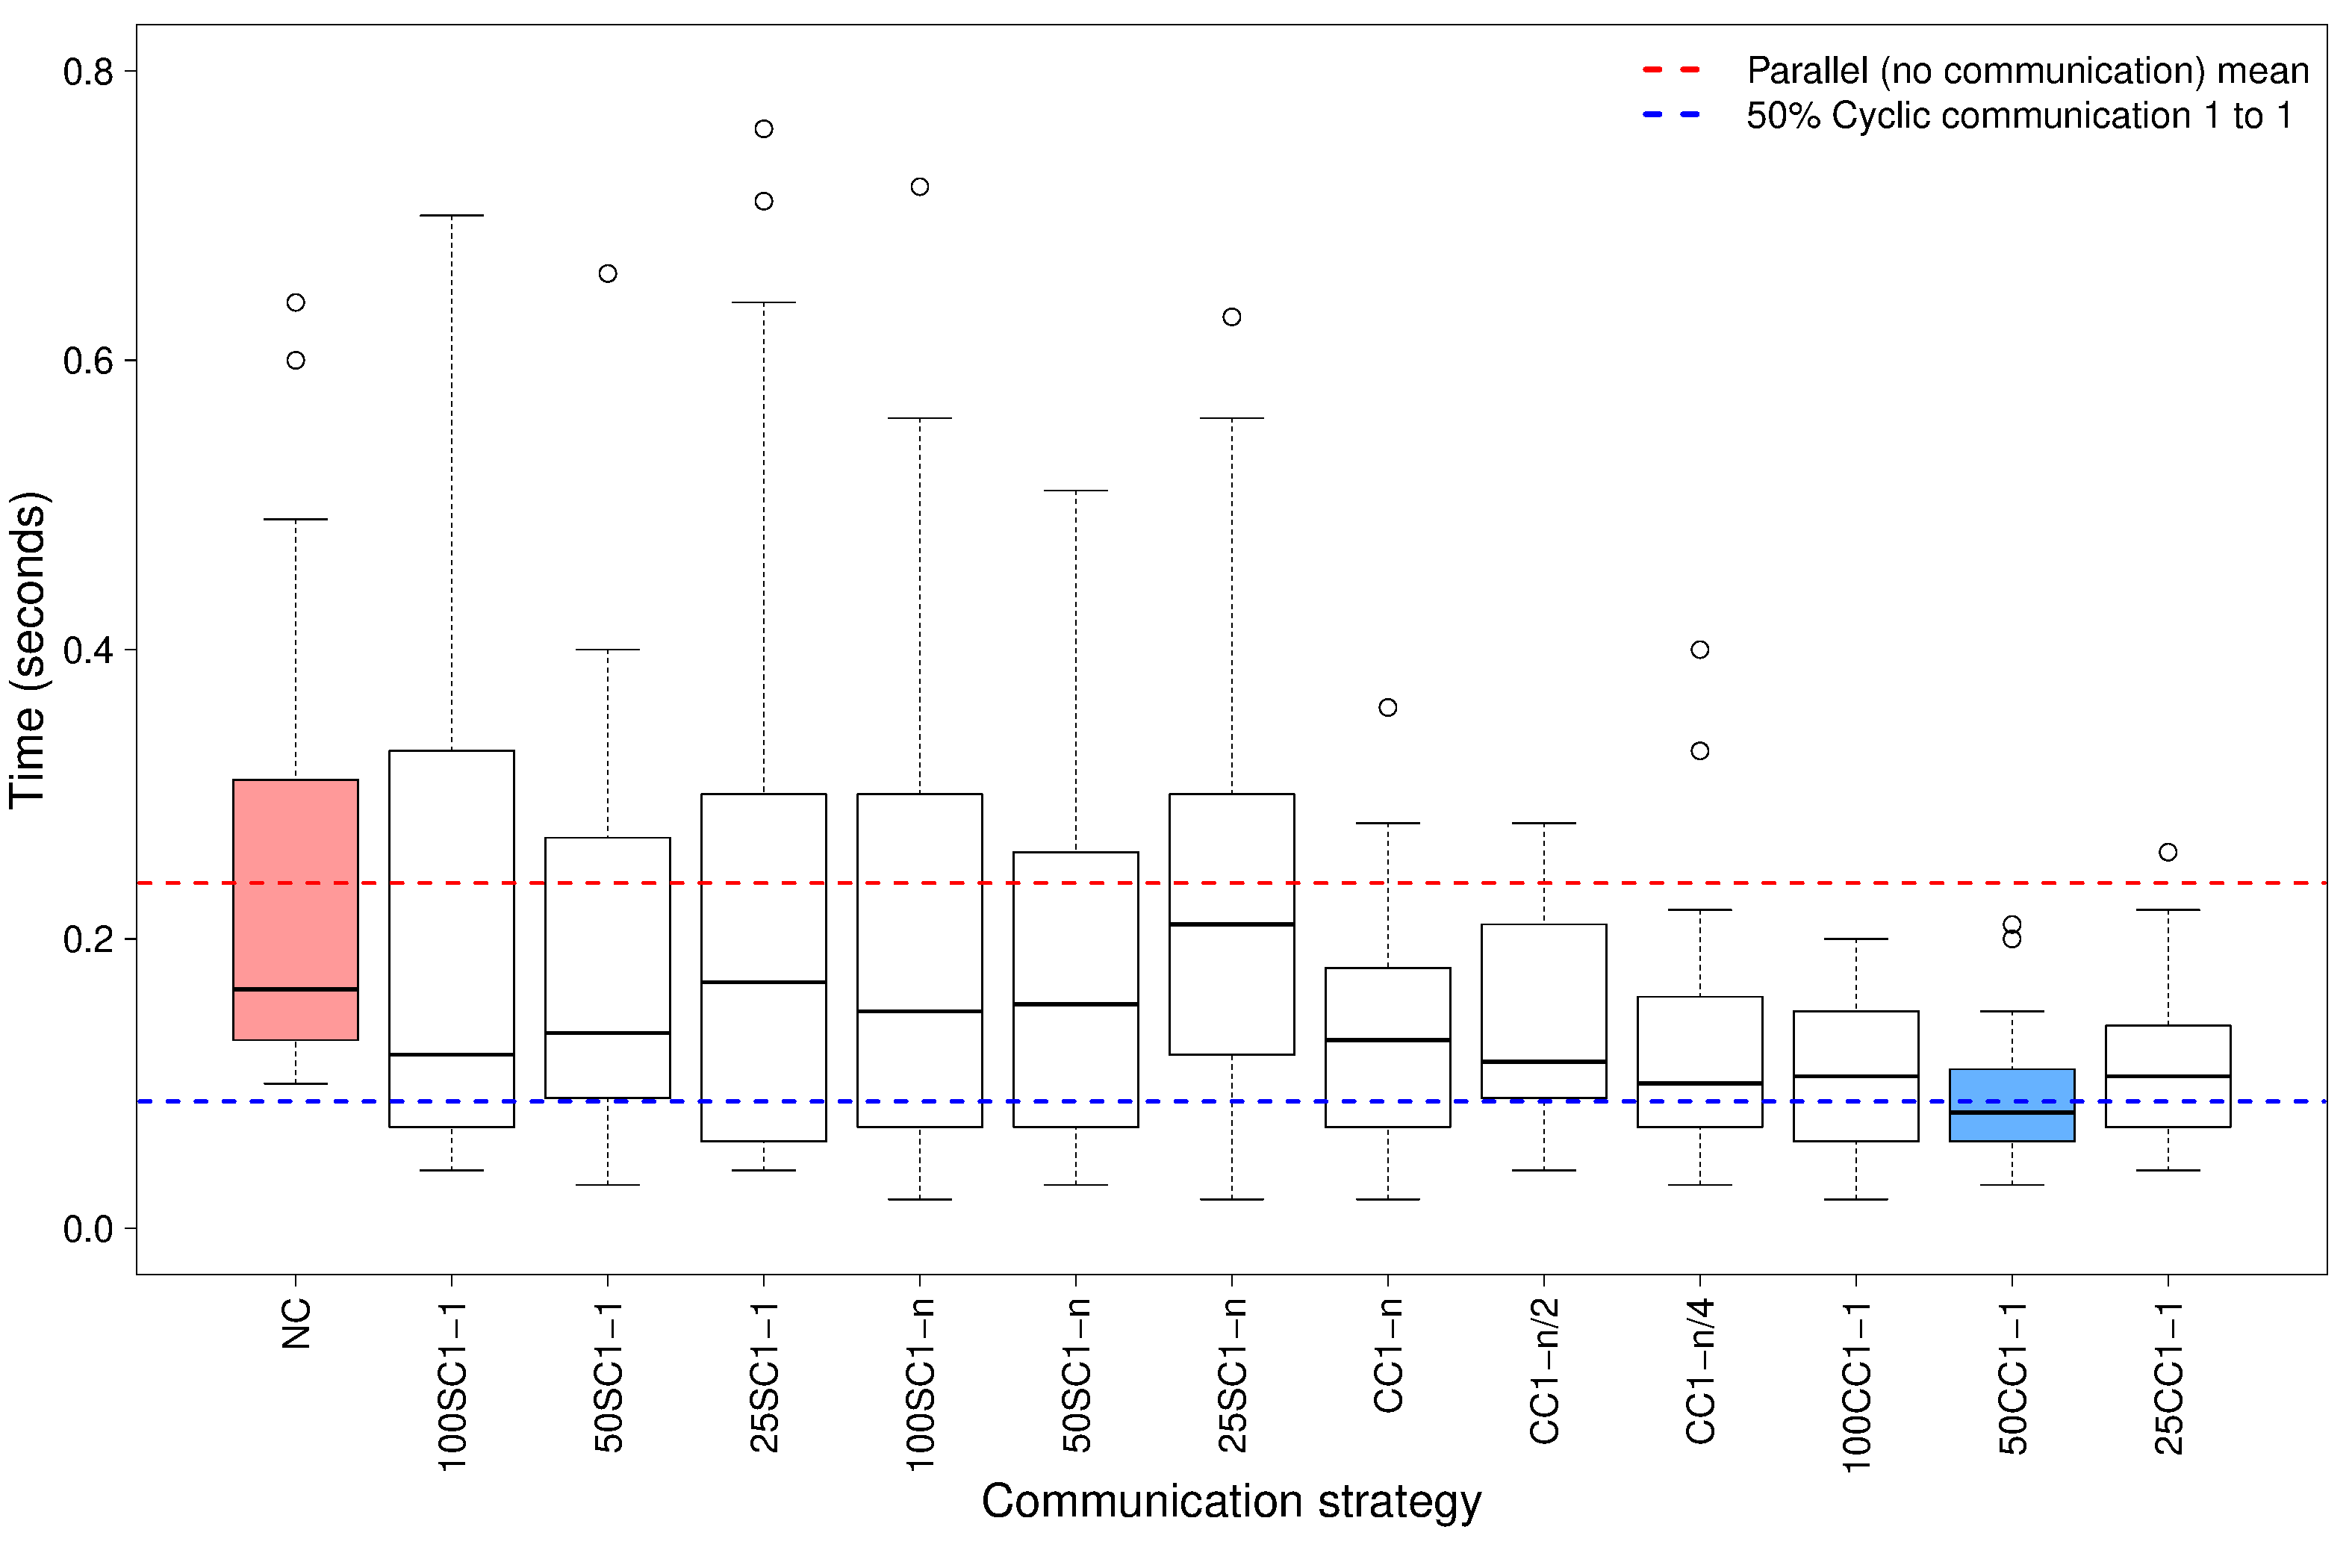
\includegraphics[width=0.8\textwidth]{g5_comm_BP.pdf}
\captionof{figure}{Different communication strategies to solve \SGP{} 5-3-7 using \posl}\label{boxplot:5comm}
\end{minipage}
%\end{figure}

\begin{minipage}[c]{\textwidth}
%\begin{figure}[h]
\centering
\includegraphics[width=0.75\textwidth]{g8_comm_BP.pdf}
\captionof{figure}{Different communication strategies to solve \SGP{} 8-4-7 using \posl}\label{boxplot:8comm}
\end{minipage}
%\end{figure}

\begin{minipage}[c]{\textwidth}
%\begin{figure}[h]
\centering
\includegraphics[width=0.75\textwidth]{g9_comm_BP.pdf}
\captionof{figure}{Different communication strategies to solve \SGP{} 9-4-8 using \posl}\label{boxplot:9comm}
%\end{figure}
\end{minipage}

%\begin{figure}[!h]
%\centering
%\includegraphics[width=0.4\textwidth]{g5_select_BP.pdf}
%\caption{Comparison between sequential and parallel (best improvement and first improvement selections) runs to solve \SGP{} 5-3-7 using \posl}
%\end{figure}

%\begin{figure}[!h]
%\centering
%\includegraphics[width=0.75\textwidth]{g8_select_BP.pdf}
%\caption{Comparison between sequential and parallel (best improvement and first improvement selections) runs to solve \SGP{} 8-4-7 using \posl}
%\end{figure}

%\begin{figure}[!h]
%\centering
%\includegraphics[width=0.75\textwidth]{g9_select_BP.pdf}
%\caption{Comparison between sequential and parallel (best improvement and first improvement selections) runs to solve \SGP{} 9-4-8 using \posl}
%\end{figure}

\section{Winner solver type representation}

Figures~\ref{barplot:5}, \ref{barplot:8} and \ref{barplot:9}, represent the percentage of winner solvers for each communication strategy, according to four different types:

\poslcaptiondesciption{
\begin{tabular}[t]{rl}
\receiver{Receiver}: & Receiver solver wining thanks to the received information \\
\sender{Sender}: & Sender solver \\
\nonreceiver{Passive receiver}: & Receiver solver wining without using the received information \\
\nocomm{Non communicating}: & Non communicating solver \\
\end{tabular}
}

In these bar graphs is evident to see how the communication has played an important role in the solution process. The number of receiver solvers which have won the search process is high, as expected, performing dynamic exchange strategies with communication \oneTn. However, due to the huge traffic of information, the communication overhead make the resulting runtimes not competitive. 

The other interesting detail showed in these graphs is that this number of winner receiver solvers remains high on winner \commstrs{} (\texttt{100\%CC1-1} and \texttt{50\%CC1-1}), achieving an important trade-off between information traffic and search speed. 

%-------- SOLVER TYPE
\begin{figure}[!h]
\centering
\includegraphics[width=0.8\textwidth]{g5_per_BP.pdf}
\caption{Solver proportion for each communication strategy to solve \SGP{} 5-3-7 using \posl}\label{barplot:5}
\end{figure}

\begin{figure}[!h]
\centering
\includegraphics[width=0.8\textwidth]{g8_per_BP.pdf}
\caption{Solver proportion for each communication strategy to solve \SGP{} 8-4-7 using \posl}\label{barplot:8}
\end{figure}

\begin{figure}[!h]
\centering
\includegraphics[width=0.8\textwidth]{g9_per_BP.pdf}
\caption{Solver proportion for each communication strategy to solve \SGP{} 9-4-8 using \posl}\label{barplot:9}
\end{figure}
%\chapter{Results of experiments with \carrp}
\label{app:cap}
\textit{This Appendix presents graphically a summary of individual runs for the \carrp. Figures show a \textit{box-plot} representation for different strategies and a bar representation for the percentage of winner solvers types.}

\vspace{2ex}\vfill
\minitoc
\newpage

\section{Comparison between sequential and parallel runs}

%\begin{wrapfigure}{R}{0.4\textwidth}
%\centering
%\includegraphics[width=0.3\textwidth]{c19_select_BP.pdf}
%\caption{Comparison between sequential and parallel runs to solve \CARRP{} 19 using \posl}\label{boxplot:19}
%\end{wrapfigure}
%
%Figure~\ref{boxplot:19} shows that the approach in parallel largely outperforms the sequential one. this is because this problem is very sensitive to the starting point. In the graph we can observe that all parallel runs are far below the mean of sequential runs. In addition, the minimum sequential runtime is higher that the 50\% of the parallel runs.

\begin{minipage}[c]{0.50\textwidth}
Figure~\ref{boxplot:19} shows that the approach in parallel largely outperforms the sequential one. This is because this problem is very sensitive to the starting point. In the graph, we can observe that all parallel runs are far below the mean of sequential runs. In addition, the minimum sequential runtime is higher that the 50\% of the parallel runs.
\end{minipage}\hspace{0.05\textwidth}
\begin{minipage}[c]{0.40\textwidth}
\centering
\includegraphics[width=0.8\textwidth]{c19_select_BP.pdf}
\captionof{figure}{Comparison between sequential and parallel runs to solve \CARRP{} 19 using \posl}\label{boxplot:19}
\end{minipage}

\section{Comparison between \commstrs}

In Figure~\ref{boxplot:comm}, labels of the x-axis correspond to the following strategies:

\poslcaptiondesciption{
\begin{tabular}[t]{rl}
\textbf{NC}: & Non communication strategy \\
\textbf{A1-1}: & 100\% of communicating solvers performing the \commstr{} A \oneTone \\
\textbf{B1-1}: & 100\% of communicating solvers performing the \commstr{} B \oneTone \\
\textbf{A1-n}: & 100\% of communicating solvers performing the \commstr{} A \oneTn \\
\textbf{B1-n}: & 100\% of communicating solvers performing the \commstr{} B \oneTn \\
\textbf{50A1-1}: & 50\% of communicating solvers performing the \commstr{} A \oneTone \\ 
\textbf{50B1-1}: & 50\% of communicating solvers performing the \commstr{} B \oneTone \\
\textbf{50A1-n}: & 50\% of communicating solvers performing the \commstr{} A \oneTn \\
\textbf{50B1-n}: & 50\% of communicating solvers performing the \commstr{} B \oneTn \\
\end{tabular}
}

Figure~\ref{boxplot:comm} shows that \commstrs{} of type \texttt{A} provide better and more stable results: the lower quartile value of parallel runs (\texttt{NC}) is higher that the upper quartile value of both \commstrs{} (\texttt{A1-1} an \texttt{A1-n})

\begin{figure}[h]
\centering
\includegraphics[width=0.8\textwidth]{c19_comm_BP.pdf}
\caption{Different communication strategies to solve \CARRP{} 19 using \posl}\label{boxplot:comm}
\end{figure} 



\section{Winner solver type representation}

Figure~\ref{barplot:19} represents the percentage of winner solvers for each communication strategy, according to three different types:

\poslcaptiondesciption{
\begin{tabular}[t]{rl}
\receiver{Receiver}: & Receiver solver wining thanks to the received information \\
\sender{Sender}: & Sender solver \\
%\nonreceiver{Pasive receiver}: & Receiver solver wining without using the received information \\
\nocomm{Non communicating}: & Non communicating solver \\
\end{tabular}
}

The bars graph in Figure~\ref{barplot:19} is self-explained: percentages of winner communicating solvers match with percentage of communicating solvers participating in the respective \commstr.

\begin{figure}[!h]
\centering
\includegraphics[width=0.6\textwidth]{c19_per_BP.pdf}
\caption{Solver proportion for each communication strategy to solve \CARRP{} 19 using \posl}\label{barplot:19}
\end{figure}
%\chapter{Results of experiments with \grp}
\label{app:grp}
\textit{This Appendix, presents graphically a summary of individuals runs using \grp. Figures show a \textit{box-plot} representation for different strategies and a bar representation for the percentage of winner solvers types.}
\vfill
\newpage

In Figures~\ref{boxplot:834comm}, \ref{boxplot:1055comm} and \ref{boxplot:1172comm}, labels of the x-axis correspond to the following strategies:
\begin{enumerate}[itemsep=-1mm]
\item \textbf{NC(noT)}: Non communication strategy without using tabu list, 
\item \textbf{NC(T)}: Non communication strategy using tabu list,
\item \textbf{C1-1}: Communicating solvers performing communication \oneTone,
\item \textbf{C1-n}: Communicating solvers performing communication \oneTn.
\end{enumerate}

Figures~\ref{barplot:834}, \ref{barplot:1055} and \ref{barplot:1172}, represent the percentage of winner solvers for each communication strategy, according to four different types:
\begin{enumerate}[itemsep=-1mm]
\item \receiver{Receiver}: Receiver solver wining thanks to the received information, 
\item \sender{Sender}: Sender solver, 
\item \nonreceiver{Pasive receiver}: Receiver solver wining without using the received information,
\end{enumerate}

\begin{figure}[!h]
\centering
\includegraphics[width=0.8\textwidth]{gol8_select_BP.pdf}
\caption{Comparison between sequential and parallel runs to solve \GRP{} 8-34 using \posl}
\end{figure}

\begin{figure}[!h]
\centering
\includegraphics[width=0.8\textwidth]{gol8_comm_BP.pdf}
\caption{Different communication strategies to solve \GRP{} 8-34 using \posl}\label{boxplot:834comm}
\end{figure}

\begin{figure}[!h]
\centering
\includegraphics[width=0.8\textwidth]{gol8_per_BP.pdf}
\caption{Solver proportion for each communication strategy to solve \GRP{} 834 using \posl}\label{barplot:834}
\end{figure}

%--------------------------------------

\begin{figure}[!h]
\centering
\includegraphics[width=0.75\textwidth]{gol10_select_BP.pdf}
\caption{Comparison between sequential and parallel runs to solve \GRP{} 10-55 using \posl}
\end{figure}

\begin{figure}[!h]
\centering
\includegraphics[width=0.75\textwidth]{gol10_comm_BP.pdf}
\caption{Different communication strategies to solve \GRP{} 10-55 using \posl}\label{boxplot:1055comm}
\end{figure}

\begin{figure}[!h]
\centering
\includegraphics[width=0.8\textwidth]{gol10_per_BP.pdf}
\caption{Solver proportion for each communication strategy to solve \GRP{} 10-55 using \posl}\label{barplot:1055}
\end{figure}

%--------------------------------------

\begin{figure}[!h]
\centering
\includegraphics[width=0.75\textwidth]{gol11_select_BP.pdf}
\caption{Comparison between sequential and parallel runs to solve \GRP{} 11-72 using \posl}
\end{figure}

\begin{figure}[!h]
\centering
\includegraphics[width=0.75\textwidth]{gol11_comm_BP.pdf}
\caption{Different communication strategies to solve \GRP{} 11-72 using \posl}\label{boxplot:1172comm}
\end{figure}

\begin{figure}[!h]
\centering
\includegraphics[width=0.8\textwidth]{gol11_per_BP.pdf}
\caption{Solver proportion for each communication strategy to solve \GRP{} 11-72 using \posl}\label{barplot:1172}
\end{figure}
%\chapter{Results of experiments with \nqp}
\label{app:nqp}
\textit{This Appendix, presents graphically a summary of individuals runs using \nqp. Figures show a \textit{box-plot} representation for different strategies and a bar representation for the percentage of winner solvers types.}
\vfill
\newpage

In Figures~\ref{boxplot:250}, \ref{boxplot:500}, \ref{boxplot:1000}, \ref{boxplot:3000} and~\ref{boxplot:6000}, labels of the x-axis correspond to the following strategies:

\poslcaptiondesciption{
\begin{tabular}[t]{rl}
\textbf{Seq}: & Sequential strategy (1 core)\\
\textbf{NC}: & Parallel non communicative strategy\\
\textbf{Cyc1-1}: & Cyclic communicating strategy with communication \oneTone \\
\textbf{Cyc1-n}: & Cyclic communicating strategy with communication \oneTn \\
\textbf{S1-1}: & Simple communicating strategy with communication \oneTone \\
\textbf{S1-n}: & One set of solvers performing a simple communicating strategy with communication \oneTone \\
\textbf{S1-n/2}: & Two sets of solvers performing a simple communicating strategy with communication \oneTone \\
\textbf{S1-n/4}: & Four sets of solvers performing a simple communicating strategy with communication \oneTone \\
\end{tabular}
}

Figures~\ref{barplot:250}, \ref{barplot:500}, \ref{barplot:1000}, \ref{barplot:3000} and \ref{barplot:6000}, represent the percentage of winner solvers for each communication strategy, according to four different types:

\poslcaptiondesciption{
\begin{tabular}[t]{rl}
\receiver{Receiver}: & Receiver solver wining thanks to the received information \\
\sender{Sender}: & Sender solver \\
\nonreceiver{Pasive receiver}: & Receiver solver wining without using the received information \\
%\textbf{Non communicating}: & Non communicating solver \\
\end{tabular}
}

%------ COMMUNICATION
\begin{figure}[!h]
\centering
\includegraphics[width=0.8\textwidth]{nq250_BP.pdf}
\caption{Different communication strategies to solve 250-Queens using \posl}\label{boxplot:250}
\end{figure}

\begin{figure}[!h]
\centering
\includegraphics[width=0.8\textwidth]{nq500_BP.pdf}
\caption{Different communication strategies to solve 500-Queens using \posl}\label{boxplot:500}
\end{figure}

\begin{figure}[!h]
\centering
\includegraphics[width=0.8\textwidth]{nq1000_BP.pdf}
\caption{Different communication strategies to solve 1000-Queens using \posl}\label{boxplot:1000}
\end{figure}

\begin{figure}[!h]
\centering
\includegraphics[width=0.8\textwidth]{nq3000_BP.pdf}
\caption{Different communication strategies to solve 3000-Queens using \posl}\label{boxplot:3000}
\end{figure}

\begin{figure}[!h]
\centering
\includegraphics[width=0.8\textwidth]{nq6000_BP.pdf}
\caption{Different communication strategies to solve 6000-Queens using \posl}\label{boxplot:6000}
\end{figure}

%-------- SOLVER TYPE
\begin{figure}[!h]
\centering
\subfloat[][\NQP{} 250 ]{
	\label{barplot:250}
	\includegraphics[width=0.5\linewidth]{nq250_per_BP.pdf}
} %\hspace{0.05\linewidth}
\subfloat[][\NQP{} 500 ]{%
	\label{barplot:500}
	\includegraphics[width=0.5\linewidth]{nq500_per_BP.pdf}
}\\
\subfloat[][\NQP{} 1000 ]{
	\label{barplot:1000}
	\includegraphics[width=0.5\linewidth]{nq1000_per_BP.pdf}
} %\hspace{0.05\linewidth}
\subfloat[][\NQP{} 3000 ]{%
	\label{barplot:3000}
	\includegraphics[width=0.5\linewidth]{nq3000_per_BP.pdf}
}
\caption[]{Solver proportion for each communication strategy to solve \NQP{} using \posl}
\label{fig:bars_nq}
\end{figure}

\begin{figure}[!h]
\centering
\includegraphics[width=0.5\textwidth]{nq6000_per_BP.pdf}
\caption{Solver proportion for each communication strategy to solve \NQP{} using \posl}\label{barplot:6000}
\end{figure}
%\chapter{Results of experiments with \nqp}
\label{app:nqp}
\textit{In this appendix results values of experiments with \nqp{} are presented.}
\vfill
\newpage

Column labels:
\begin{itemize}
\item \texttt{Sequential}: Experiment using one core.
\item \texttt{Parallel}: Experiment using 40 cores without communication.
\item \texttt{K \% / com. 1-1}: Experiment with $K$\% of communicating solvers ($\tfrac{K}{2}$\% of sender solvers, and $\tfrac{K}{2}$\% of receiver solvers) using communication \textit{one~to~one}, and $100-K$\% of non-communicating solvers.
\item \texttt{K \% / com. 1-N}: Experiment with $K$\% of communicating solvers ($\tfrac{K}{2}$\% of sender solvers, and $\tfrac{K}{2}$\% of receiver solvers) using communication \textit{one~to~N}, and $100-K$\% of non-communicating solvers.
\item \texttt{Time}: Time in milliseconds. 
\item \texttt{Iter.}: Number of iterations.
\end{itemize}

Color caption:
\begin{itemize}
\item \gracias{Values in red color}: A receiver solver was the winner, finding the solution thanks to the received information.
\item \receiver{Values in dark red color}: A receiver solver was the winner, finding the solution without tacking into account the received information.
\item \sender{Values in blue color}: A sender solver was the winner.
\item \nocomm{Values in black color}: A non-communicating solver was the winner.
\end{itemize}

%\noindent\rule[2pt]{\textwidth}{0.8pt}

\clearpage
\includepdf[pages=-]{appres//res_nqueens.pdf}
%\chapter{Results of experiments with \carrp}
\label{app:cap}
\textit{In this appendix results values of experiments with \carrp{} are presented.}
\vfill
\newpage

Column labels:
\begin{itemize}
\item \texttt{Sequential}: Experiment using one core.
\item \texttt{No Communication}: Experiment using 40 cores without communication.
\item \texttt{St\_S / K \% com. OP}: Experiment with $K$\% of communicating solvers ($\tfrac{K}{2}$\% of sender solvers, and $\tfrac{K}{2}$\% of receiver solvers) using the communication strategy $S$ and the communication operator $OP$, and $100-K$\% of non-communicating solvers.
\begin{itemize}
\item Communication strategy:
	\begin{itemize}
	\item $S = a$: communication performed while applying the acceptance criteria 
	\item $S = b$: communication performed while performing a {\it reset} (each $k$ iterations)
	\item $S = c$: communication performed while performing a {\it reset} (each iteration)
	\end{itemize}
\item Communication operator:
	\begin{itemize}
	\item $OP = $ \texttt{1-1}: communication operator \texttt{one~to~one}
	\item $OP = $ \texttt{1-n}: communication operator \texttt{one~to~n}
	\end{itemize}
\end{itemize}
\item \texttt{Time}: Time in milliseconds. 
\item \texttt{Iter.}: Number of iterations.
\end{itemize}

Color caption:
\begin{itemize}
\item \gracias{Values in red color}: A receiver solver was the winner, finding the solution thanks to the received information.
\item \receiver{Values in dark red color}: A receiver solver was the winner, finding the solution without tacking into account the received information.
\item \sender{Values in blue color}: A sender solver was the winner.
\item \nocomm{Values in black color}: A non-communicating solver was the winner.
\end{itemize}

%\noindent\rule[2pt]{\textwidth}{0.8pt}

\clearpage
\includepdf[pages=-]{appres//res_costas.pdf}
%\chapter{Results of experiments with \grp}
\label{app:grp}
\textit{In this appendix results values of experiments with \grp{} are presented.}
\vfill
\newpage

Column labels:
\begin{itemize}
\item \texttt{Using Tabu List (no communication)}: Experiment in parallel using a global tabu list.
\item \texttt{Without Tabu List (no communication)}: Experiment in parallel without using a global tabu list.
\item \texttt{Using Tabu List (communication 1-1)}: Experiment in parallel using a global tabu list and communication \textit{one~to~one}.
\item \texttt{Using Tabu List (communication 1-n)}: Experiment in parallel using a global tabu list and communication \textit{one~to~N}.
\item \texttt{Sequential (without tabu list)}: Experiment using one core and without tabu list.
\item \texttt{Sequential (with tabu list)}: Experiment using one core and a global tabu list.
\item \texttt{time}: Time in milliseconds. 
\item \texttt{iterations}: Number of iterations.
\item \texttt{restarts}: Number of restarts performed by the winner solver.
\end{itemize}

Color caption:
\begin{itemize}
\item \gracias{Values in red color}: A receiver solver was the winner, finding the solution thanks to the received information.
\item \sender{Values in blue color}: A sender solver was the winner.
\item \nocomm{Values in black color}: A non-communicating solver was the winner.
\end{itemize}

Other captions:
\begin{itemize}
\item \texttt{Eps}: The gap ($\epsilon$) used to consider a configuration near enough to a possible local minimum.
\item \texttt{Norm}: The vector norm type used to compute the mentioned gap.
\item \nocomm{tabu size}: The capacity of the global tabu list.
\end{itemize}

%\noindent\rule[2pt]{\textwidth}{0.8pt}

\clearpage
\includepdf[pages=-]{appres//res_golomb.pdf}
%\chapter{\posl{} Class diagrams}
\label{app:diag}
\textit{In this appendix are presented the class diagrams of the current implementation of \posl\footnote{\posl's source code is abailable at \href{https://github.com/alejandro-reyesamaro/POSL}{https://github.com/alejandro-reyesamaro/POSL}}. In these diagrams are shown only the most important classes (and fields) that were used during the experimentation process for this thesis, in order to facilitate the understanding of the class design.}
\vfill
\newpage


%\noindent\rule[2pt]{\textwidth}{0.8pt}

\clearpage

%\begin{figure}
%	\centering
%	\subfloat[][Data \opch]{
%		\label{subfig:doch}
%		\includegraphics[width=0.4\linewidth]{D_OCh.png}
%	}
%	\hspace{0.05\textwidth}%
%	\subfloat[][Object \opch]{%
%		\label{subfig:ooch}
%		\includegraphics[width=0.4\linewidth]{O_OCh.png}
%	}
%	\caption[]{Communication module}
%	\label{fig:och}
%\end{figure}

\begin{figure}
	\centering
	\includegraphics[width=\linewidth]{diabench.png}
	\caption[]{Benchmark class diagram}\label{diag:bench}
\end{figure}

\begin{figure}
	\centering
	\includegraphics[width=\linewidth]{diacoststr.png}
	\caption[]{Cost strategy class diagram}\label{diag:coststr}
\end{figure}

\begin{figure}
	\centering
	\includegraphics[width=\linewidth]{diarelacoststr.png}
	\caption[]{Relative cost strategy class diagram}\label{diag:relacoststr}
\end{figure}

\begin{figure}
	\centering
	\includegraphics[width=\linewidth]{diashowstr.png}
	\caption[]{Show solution strategy class diagram}\label{diag:showstr}
\end{figure}

\begin{figure}
	\centering
	\includegraphics[width=\linewidth]{diadata.png}
	\caption[]{\posl{} data class diagram}\label{diag:data}
\end{figure}

\begin{figure}
	\centering
	\includegraphics[width=\linewidth]{diacm.png}
	\caption[]{Compound modules class diagram}\label{diag:cm}
\end{figure}

\begin{figure}
	\centering
	\includegraphics[width=\linewidth]{diaom.png}
	\caption[]{Abstract computation modules class diagram}\label{diag:om}
\end{figure}

\begin{figure}
	\centering
	\includegraphics[width=\linewidth]{diaoch.png}
	\caption[]{Communication modules class diagram}\label{diag:opch}
\end{figure}

\begin{figure}
	\centering
	\includegraphics[width=\linewidth]{diaaomacc.png}
	\caption[]{Acceptance computation modules class diagram}\label{diag:accmodules}
\end{figure}

\begin{figure}
	\centering
	\includegraphics[width=\linewidth]{diaaomneigh.png}
	\caption[]{Neighborhood computation modules class diagram}\label{diag:neighmodules}
\end{figure}

\begin{figure}
	\centering
	\includegraphics[width=\linewidth]{diaaomselect.png}
	\caption[]{Selection computation modules class diagram}\label{diag:selectmodules}
\end{figure}

\begin{figure}
	\centering
	\includegraphics[width=\linewidth]{diaaomgen.png}
	\caption[]{Generation computation modules class diagram}\label{diag:genmodules}
\end{figure}

\begin{figure}
	\centering
	\includegraphics[width=\linewidth]{diaaomproconf.png}
	\caption[]{Processing solution computation modules class diagram}\label{diag:procconfmodules}
\end{figure}

\begin{figure}
	\centering
	\includegraphics[width=\linewidth]{diaaomproset.png}
	\caption[]{Processing configuration--set computation modules class diagram}\label{diag:procsetmodules}
\end{figure}

\begin{figure}
	\centering
	\includegraphics[width=\linewidth]{diaoperator.png}
	\caption[]{Operator class diagram}\label{diag:operator}
\end{figure}

\begin{figure}
	\centering
	\includegraphics[width=\linewidth]{diaseqoper.png}
	\caption[]{Operator sequential strategy class diagram}\label{diag:seqoperstr}
\end{figure}

\begin{figure}
	\centering
	\includegraphics[width=\linewidth]{diaparoper.png}
	\caption[]{Operator parallel strategy class diagram}\label{diag:paroperstr}
\end{figure}

\begin{figure}
	\centering
	\includegraphics[width=\linewidth]{diasolverset.png}
	\caption[]{Solver Set class diagram}\label{diag:solverset}
\end{figure}

\clearpage 

\begin{figure}
	\centering
	\includegraphics[width=\linewidth]{diaresultshowing.png}
	\caption[]{Showing result class diagram}\label{diag:showingres}
\end{figure}

\begin{figure}
	\centering
	\includegraphics[width=\linewidth]{diacommoperator.png}
	\caption[]{Communication operator class diagram}\label{diag:commoper}
\end{figure}
%\cleardoublepage
\begin{titlepage}
    \vspace*{\fill}
    \begin{center}
      {\LARGE \textbf{Paper I}}\\[0.5cm]
      {\Large \textit{In which we review the field of quantitative FRET...}}\\[0.4cm]
    \end{center}
    \vspace*{\fill}
  \end{titlepage}
\cleardoublepage
\includepdf[pages=-]{adds//CBC2012.pdf}

\cleardoublepage
\begin{titlepage}
    \vspace*{\fill}
    \begin{center}
      {\LARGE \textbf{Paper II}}\\[0.5cm]
      {\Large \textit{In which tC$_{nitro}$ is characterized as a FRET acceptor...}}\\[0.4cm]
    \end{center}
    \vspace*{\fill}
  \end{titlepage}
\cleardoublepage
\includepdf[pages=-]{adds//JPCB2010.pdf}

\cleardoublepage
\begin{titlepage}
    \vspace*{\fill}
    \begin{center}
      {\LARGE \textbf{Paper III}}\\[0.5cm]
      {\Large \textit{In which FRETmatrix is presented...}}\\[0.4cm]
    \end{center}
    \vspace*{\fill}
  \end{titlepage}
\cleardoublepage
\includepdf[pages=-]{adds//NAR2012.pdf}
\includepdf[pages=-]{adds//NAR2012_sup.pdf}

\cleardoublepage
\begin{titlepage}
    \vspace*{\fill}
    \begin{center}
      {\LARGE \textbf{Paper IV}}\\[0.5cm]
      {\Large \textit{In which we present a multistate, reversible switch based on a functionalized DNA hairpin loop...}}\\[0.4cm]
    \end{center}
    \vspace*{\fill}
  \end{titlepage}
\cleardoublepage
\includepdf[pages=-]{adds//CC2012.pdf}
\includepdf[pages=-]{adds//CC2012_sup.pdf}

\cleardoublepage
\begin{titlepage}
    \vspace*{\fill}
    \begin{center}
      {\LARGE \textbf{Paper V}}\\[0.5cm]
      {\Large \textit{In which we gain structural and electronic insight into the tC probes...}}\\[0.4cm]
    \end{center}
    \vspace*{\fill}
  \end{titlepage}
\cleardoublepage
\includepdf[pages=-]{adds//PCCP2010.pdf}
\includepdf[pages=-]{adds//PCCP2010_sup.pdf}

\cleardoublepage
\begin{titlepage}
    \vspace*{\fill}
    \begin{center}
      {\LARGE \textbf{Paper VI}}\\[0.5cm]
      {\Large \textit{In which a new fluorescent adenine analogue is presented...}}\\[0.4cm]
    \end{center}
    \vspace*{\fill}
  \end{titlepage}
\cleardoublepage
\includepdf[pages=-]{adds//CEJ2012.pdf}


\end{document}